%&preformat-disser
\RequirePackage[l2tabu,orthodox]{nag} % Раскомментировав, можно в логе получать рекомендации относительно правильного использования пакетов и предупреждения об устаревших и нерекомендуемых пакетах
% Формат А4, 14pt (ГОСТ Р 7.0.11-2011, 5.3.6)
\documentclass[a4paper,14pt,oneside,openany]{memoir}

%%%%%%%%%%%%%%%%%%%%%%%%%%%%%%%%%%%%%%%%%%%%%%%%%%%%%%%%%%%%%%%%%%%%%%%%%%%%%%%%
%%%% Файл упрощённых настроек шаблона, общих для диссертации и автореферата %%%%
%%%%%%%%%%%%%%%%%%%%%%%%%%%%%%%%%%%%%%%%%%%%%%%%%%%%%%%%%%%%%%%%%%%%%%%%%%%%%%%%

%%% Режим черновика %%%
\makeatletter
\@ifundefined{c@draft}{
  \newcounter{draft}
  \setcounter{draft}{0}  % 0 --- чистовик (максимальное соблюдение ГОСТ)
                         % 1 --- черновик (отклонения от ГОСТ, но быстрая
                         %       сборка итоговых PDF)
}{}
\makeatother

%%% Пометки в тексте %%%
\makeatletter
\@ifundefined{c@showmarkup}{
  \newcounter{showmarkup}
  \setcounter{showmarkup}{0}  % 0 --- скрыть пометки
                              % 1 --- показывать пометки
}{}
\makeatother

%%% Использование в pdflatex шрифтов не по-умолчанию %%%
\makeatletter
\@ifundefined{c@usealtfont}{
  \newcounter{usealtfont}
  \setcounter{usealtfont}{1}    % 0 --- шрифты на базе Computer Modern
                                % 1 --- использовать пакет pscyr, при его
                                %       наличии
                                % 2 --- использовать пакет XCharter, при наличии
                                %       подходящей версии
}{}
\makeatother

%%% Использование в xelatex и lualatex семейств шрифтов %%%
\makeatletter
\@ifundefined{c@fontfamily}{
  \newcounter{fontfamily}
  \setcounter{fontfamily}{1}  % 0 --- CMU семейство. Используется как fallback;
                              % 1 --- Шрифты от MS (Times New Roman и компания)
                              % 2 --- Семейство Liberation
}{}
\makeatother

%%% Библиография %%%
\makeatletter
\@ifundefined{c@bibliosel}{
  \newcounter{bibliosel}
  \setcounter{bibliosel}{1}   % 0 --- встроенная реализация с загрузкой файла
                              %       через движок bibtex8;
                              % 1 --- реализация пакетом biblatex через движок
                              %       biber
}{}
\makeatother

%%% Вывод типов ссылок в библиографии %%%
\makeatletter
\@ifundefined{c@mediadisplay}{
  \newcounter{mediadisplay}
  \setcounter{mediadisplay}{2}   % 0 --- не делать ничего; надписи [Текст] и
                                 %       [Эл. ресурс] будут выводиться только в ссылках с
                                 %       заполненным полем `media`;
                                 % 1 --- автоматически добавлять надпись [Текст] к ссылкам с
                                 %       незаполненным полем `media`; таким образом, у всех
                                 %       источников будет указан тип, что соответствует
                                 %       требованиям ГОСТ
                                 % 2 --- автоматически удалять надписи [Текст], [Эл. Ресурс] и др.;
                                 %       не соответствует ГОСТ
                                 % 3 --- автоматически удалять надпись [Текст];
                                 %       не соответствует ГОСТ
                                 % 4 --- автоматически удалять надпись [Эл. Ресурс];
                                 %       не соответствует ГОСТ
}{}
\makeatother

%%% Предкомпиляция tikz рисунков для ускорения работы %%%
\makeatletter
\@ifundefined{c@imgprecompile}{
  \newcounter{imgprecompile}
  \setcounter{imgprecompile}{0}   % 0 --- без предкомпиляции;
                                  % 1 --- пользоваться предварительно
                                  %       скомпилированными pdf вместо генерации
                                  %       заново из tikz
}{}
\makeatother
            % общие настройки шаблона
%%% Проверка используемого TeX-движка %%%
\newif\ifxetexorluatex   % определяем новый условный оператор (http://tex.stackexchange.com/a/47579)
\ifxetex
    \xetexorluatextrue
\else
    \ifluatex
        \xetexorluatextrue
    \else
        \xetexorluatexfalse
    \fi
\fi

\newif\ifsynopsis           % Условие, проверяющее, что документ --- автореферат

\usepackage{etoolbox}[2015/08/02]   % Для продвинутой проверки разных условий
\providebool{presentation}

\usepackage{comment}    % Позволяет убирать блоки текста (добавляет
                        % окружение comment и команду \excludecomment)

%%% Поля и разметка страницы %%%
\usepackage{pdflscape}  % Для включения альбомных страниц
\usepackage{geometry}   % Для последующего задания полей

%%% Математические пакеты %%%
\usepackage{amsthm,amsmath,amscd}   % Математические дополнения от AMS
\usepackage{amsfonts,amssymb}       % Математические дополнения от AMS
\usepackage{mathtools}              % Добавляет окружение multlined
\usepackage{xfrac}                  % Красивые дроби
\usepackage[
    locale = DE,
    list-separator       = {;\,},
    list-final-separator = {;\,},
    list-pair-separator  = {;\,},
    list-units           = single,
    range-units          = single,
    range-phrase={\text{\ensuremath{-}}},
    % quotient-mode        = fraction, % красивые дроби могут не соответствовать ГОСТ
    fraction-function    = \sfrac,
    separate-uncertainty,
    ]{siunitx}[=v2]                 % Размерности SI
\sisetup{inter-unit-product = \ensuremath{{}\cdot{}}}

% Кириллица в нумерации subequations
% Для правильной работы требуется выполнение сразу после загрузки пакетов
\patchcmd{\subequations}{\def\theequation{\theparentequation\alph{equation}}}
{\def\theequation{\theparentequation\asbuk{equation}}}
{\typeout{subequations patched}}{\typeout{subequations not patched}}

%%%% Установки для размера шрифта 14 pt %%%%
%% Формирование переменных и констант для сравнения (один раз для всех подключаемых файлов)%%
%% должно располагаться до вызова пакета fontspec или polyglossia, потому что они сбивают его работу
\newlength{\curtextsize}
\newlength{\bigtextsize}
\setlength{\bigtextsize}{13.9pt}

\makeatletter
%\show\f@size    % неплохо для отслеживания, но вызывает стопорение процесса,
                 % если документ компилируется без команды  -interaction=nonstopmode
\setlength{\curtextsize}{\f@size pt}
\makeatother

%%% Кодировки и шрифты %%%
\ifxetexorluatex
    \ifpresentation
        \providecommand*\autodot{} % quick fix for polyglossia 1.50
    \fi
    \PassOptionsToPackage{no-math}{fontspec}    % https://tex.stackexchange.com/a/26295/104425
    \usepackage{polyglossia}[2014/05/21]        % Поддержка многоязычности
                                        % (fontspec подгружается автоматически)
\else
   %%% Решение проблемы копирования текста в буфер кракозябрами
    \ifnumequal{\value{usealtfont}}{0}{}{
        \input glyphtounicode.tex
        \input glyphtounicode-cmr.tex %from pdfx package
        \pdfgentounicode=1
    }
    \usepackage{cmap}   % Улучшенный поиск русских слов в полученном pdf-файле
    \ifnumequal{\value{usealtfont}}{2}{}{
        \defaulthyphenchar=127  % Если стоит до fontenc, то переносы
                                % не впишутся в выделяемый текст при
                                % копировании его в буфер обмена
    }
    \usepackage{textcomp}
    \usepackage[T1,T2A]{fontenc}                    % Поддержка русских букв
    \ifnumequal{\value{usealtfont}}{1}{% Используется pscyr, при наличии
        \IfFileExists{pscyr.sty}{\usepackage{pscyr}}{}  % Подключение pscyr
    }{}
    \usepackage[utf8]{inputenc}[2014/04/30]         % Кодировка utf8
    \usepackage[english, russian]{babel}[2014/03/24]% Языки: русский, английский
    \makeatletter\AtBeginDocument{\let\@elt\relax}\makeatother % babel 3.40 fix
    \ifnumequal{\value{usealtfont}}{2}{
        % http://dxdy.ru/post1238763.html#p1238763
        \usepackage[scaled=0.914]{XCharter}[2017/12/19] % Подключение русифицированных шрифтов XCharter
        \usepackage[charter, vvarbb, scaled=1.048]{newtxmath}[2017/12/14]
        \ifpresentation
        \else
            \setDisplayskipStretch{-0.078}
        \fi
    }{}
\fi

%%% Оформление абзацев %%%
\ifpresentation
\else
    \indentafterchapter     % Красная строка после заголовков типа chapter
    \usepackage{indentfirst}
\fi

%%% Цвета %%%
\ifpresentation
\else
    \usepackage[dvipsnames, table, hyperref]{xcolor} % Совместимо с tikz
\fi

%%% Таблицы %%%
\usepackage{longtable,ltcaption} % Длинные таблицы
\usepackage{multirow,makecell}   % Улучшенное форматирование таблиц
\usepackage{tabu, tabulary}      % таблицы с автоматически подбирающейся
                                 % шириной столбцов (tabu обязательно
                                 % до hyperref вызывать)
\makeatletter
%https://github.com/tabu-issues-for-future-maintainer/tabu/issues/26
\@ifpackagelater{longtable}{2020/02/07}{
\def\tabuendlongtrial{%
    \LT@echunk  \global\setbox\LT@gbox \hbox{\unhbox\LT@gbox}\kern\wd\LT@gbox
                \LT@get@widths
}%
}{}
\makeatother

\usepackage{threeparttable}      % автоматический подгон ширины подписи таблицы

%%% Общее форматирование
%\usepackage{soulutf8}% Поддержка переносоустойчивых подчёркиваний и зачёркиваний
\usepackage{soul}
\usepackage{icomma}  % Запятая в десятичных дробях

%%% Оптимизация расстановки переносов и длины последней строки абзаца
\IfFileExists{impnattypo.sty}{% проверка установленности пакета impnattypo
    \ifluatex
        \ifnumequal{\value{draft}}{1}{% Черновик
            \usepackage[hyphenation, lastparline, nosingleletter, homeoarchy,
            rivers, draft]{impnattypo}
        }{% Чистовик
            \usepackage[hyphenation, lastparline, nosingleletter]{impnattypo}
        }
    \else
        \usepackage[hyphenation, lastparline]{impnattypo}
    \fi
}{}

%% Векторная графика

\usepackage{tikz}                   % Продвинутый пакет векторной графики
\usetikzlibrary{chains}             % Для примера tikz рисунка
\usetikzlibrary{shapes.geometric}   % Для примера tikz рисунка
\usetikzlibrary{shapes.symbols}     % Для примера tikz рисунка
\usetikzlibrary{arrows}             % Для примера tikz рисунка

%%% Гиперссылки %%%
\ifxetexorluatex
    \let\CYRDZE\relax
\fi
\usepackage{hyperref}[2012/11/06]

%%% Изображения %%%
\usepackage{graphicx}[2014/04/25]   % Подключаем пакет работы с графикой
\usepackage{caption}                % Подписи рисунков и таблиц
\usepackage{subcaption}             % Подписи подрисунков и подтаблиц
\usepackage{pdfpages}               % Добавление внешних pdf файлов

%%% Счётчики %%%
\usepackage{aliascnt}
\usepackage[figure,table]{totalcount}   % Счётчик рисунков и таблиц
\usepackage{totcount}   % Пакет создания счётчиков на основе последнего номера
                        % подсчитываемого элемента (может требовать дважды
                        % компилировать документ)
\usepackage{totpages}   % Счётчик страниц, совместимый с hyperref (ссылается
                        % на номер последней страницы). Желательно ставить
                        % последним пакетом в преамбуле

%%% Продвинутое управление групповыми ссылками (пока только формулами) %%%
\ifpresentation
\else
    \usepackage[russian]{cleveref} % cleveref имеет сложности со считыванием
    % языка из babel. Такое решение русификации вывода выбрано вместо
    % определения в documentclass из опасности что-то лишнее передать во все
    % остальные пакеты, включая библиографию.

    % Добавление возможности использования пробелов в \labelcref
    % https://tex.stackexchange.com/a/340502/104425
    \usepackage{kvsetkeys}
    \makeatletter
    \let\org@@cref\@cref
    \renewcommand*{\@cref}[2]{%
        \edef\process@me{%
            \noexpand\org@@cref{#1}{\zap@space#2 \@empty}%
        }\process@me
    }
    \makeatother
\fi

\usepackage{placeins} % для \FloatBarrier

\ifnumequal{\value{draft}}{1}{% Черновик
    \usepackage[firstpage]{draftwatermark}
    \SetWatermarkText{DRAFT}
    \SetWatermarkFontSize{14pt}
    \SetWatermarkScale{15}
    \SetWatermarkAngle{45}
}{}

%%% Цитата, не приводимая в автореферате:
% возможно, актуальна только для biblatex
%\newcommand{\citeinsynopsis}[1]{\ifsynopsis\else ~\cite{#1} \fi}

% если текущий процесс запущен библиотекой tikz-external, то прекомпиляция должна быть включена
\ifdefined\tikzexternalrealjob
    \setcounter{imgprecompile}{1}
\fi

\ifnumequal{\value{imgprecompile}}{1}{% Только если у нас включена предкомпиляция
    \usetikzlibrary{external}   % подключение возможности предкомпиляции
    \tikzexternalize[prefix=images/cache/,optimize command away=\includepdf] % activate! % здесь можно указать отдельную папку для скомпилированных файлов
    \ifxetex
        \tikzset{external/up to date check={diff}}
    \fi
}{}


% пакеты пользователя
\usepackage{epigraph}
\usepackage{mathtools}



% КОМАНДЫ ПОЛЬЗОВАТЕЛЯ

% множества
\newcommand{\EE}{\mathbb{E}}
\newcommand{\NN}{\mathbb{N}}
\newcommand{\ZZ}{\mathbb{Z}}
\newcommand{\FF}{\mathbb{F}}
% группы, квазигруппы
\newcommand{\SSS}{\mathcal{S}}
\newcommand{\sprop}{\mathcal{S}^{\mathsf{prop}}}
\newcommand{\QQQ}{Q_1 \times \ldots \times Q_n}
\newcommand{\GGG}{G}

% функции и аргументы
\newcommand{\ff}{\mathcal{F}}
\newcommand{\gf}{\mathcal{G}}
\newcommand{\hf}{\mathcal{H}}
\renewcommand{\ss}{\mathbf{s}}
\newcommand{\xx}{\mathbf{x}}
\newcommand{\yy}{\mathbf{y}}
%\newcommand{\zz}{\mathbf{z}}
\newcommand{\uu}{\mathbf{u}}
\newcommand{\vv}{\mathbf{v}}
\newcommand{\ww}{\mathbf{w}}
\newcommand{\dd}{\partial}
\newcommand{\loc}{\mathsf{loc}}
\newcommand{\rec}{\mathsf{rec}}
\newcommand{\hupf}{\mathsf{HUFP}}
\newcommand{\divides}{\mid}

% команды 
\newcommand{\proj}{\Pi}
\newcommand{\inv}{\mathsf{inv}}
\newcommand{\Img}{\mathsf{Im}}
\newcommand{\fib}{\mathsf{Fib}}
\newcommand{\lucas}{\mathsf{Lucas}}
\newcommand{\uso}{\mathsf{USO}}


% криптография
\newcommand{\sample}{\gets^{\mathcal{U}}}
\newcommand{\Dom}{\mathbf{Dom}}
\newcommand{\Keys}{\mathbf{Keys}}
\newcommand{\Twk}{\mathbf{Twk}}
\newcommand{\enc}{\mathsf{Enc}}
\newcommand{\dec}{\mathsf{Dec}}
\newcommand{\gen}{\mathsf{Gen}}
\newcommand{\fpe}{\mathsf{FPE}}

\DeclareMathOperator*\uplim{\overline{lim}}

% etc commands
\newcommand{\TODO}[1]{{\color{red}{\textbf{ TODO: #1}}}}
\newcommand{\COMMENT}[1]{{\color{blue}{\textbf{ COMMENT: #1}}}}

\renewcommand{\mod}{\text{ mod }}

%\renewcommand{\labelitemii}{$\circ$}


\newtheorem{Algo}{Алгоритм}

         % Пакеты общие для диссертации и автореферата
\synopsisfalse                      % Этот документ --- не автореферат
%%% Прикладные пакеты %%%
%\usepackage{calc}               % Пакет для расчётов параметров, например длины

%%% Для добавления Стр. над номерами страниц в оглавлении
%%% http://tex.stackexchange.com/a/306950
\usepackage{afterpage}

%%% Списки %%%
\usepackage{enumitem}

%%% Оформление списка обозначений
\usepackage[intoc]{nomencl}
\makenomenclature
\setlength{\nomitemsep}{-.8\parsep}
    % Пакеты для диссертации
\usepackage{fr-longtable}    %ради \endlasthead

% Листинги с исходным кодом программ
\usepackage{fancyvrb}
\usepackage{listings}
\lccode`\~=0\relax %Без этого хака из-за особенностей пакета listings перестают работать конструкции с \MakeLowercase и т. п. в (xe|lua)latex

% Русская традиция начертания греческих букв
\usepackage{upgreek} % прямые греческие ради русской традиции

%%% Микротипографика
%\ifnumequal{\value{draft}}{0}{% Только если у нас режим чистовика
%    \usepackage[final, babel, shrink=45]{microtype}[2016/05/14] % улучшает представление букв и слов в строках, может помочь при наличии отдельно висящих слов
%}{}

% Отметка о версии черновика на каждой странице
% Чтобы работало надо в своей локальной копии по инструкции
% https://www.ctan.org/pkg/gitinfo2 создать небходимые файлы в папке
% ./git/hooks
% If you’re familiar with tweaking git, you can probably work it out for
% yourself. If not, I suggest you follow these steps:
% 1. First, you need a git repository and working tree. For this example,
% let’s suppose that the root of the working tree is in ~/compsci
% 2. Copy the file post-xxx-sample.txt (which is in the same folder of
% your TEX distribution as this pdf) into the git hooks directory in your
% working copy. In our example case, you should end up with a file called
% ~/compsci/.git/hooks/post-checkout
% 3. If you’re using a unix-like system, don’t forget to make the file executable.
% Just how you do this is outside the scope of this manual, but one
% possible way is with commands such as this:
% chmod g+x post-checkout.
% 4. Test your setup with “git checkout master” (or another suitable branch
% name). This should generate copies of gitHeadInfo.gin in the directories
% you intended.
% 5. Now make two more copies of this file in the same directory (hooks),
% calling them post-commit and post-merge, and you’re done. As before,
% users of unix-like systems should ensure these files are marked as
% executable.
\ifnumequal{\value{draft}}{1}{% Черновик
   \IfFileExists{.git/gitHeadInfo.gin}{
      \usepackage[mark,pcount]{gitinfo2}
      \renewcommand{\gitMark}{rev.\gitAbbrevHash\quad\gitCommitterEmail\quad\gitAuthorIsoDate}
      \renewcommand{\gitMarkFormat}{\rmfamily\color{Gray}\small\bfseries}
   }{}
}{}   % Пакеты для специфических пользовательских задач

%%%%%%%%%%%%%%%%%%%%%%%%%%%%%%%%%%%%%%%%%%%%%%%%%%%%%%
%%%% Файл упрощённых настроек шаблона диссертации %%%%
%%%%%%%%%%%%%%%%%%%%%%%%%%%%%%%%%%%%%%%%%%%%%%%%%%%%%%

%%% Инициализирование переменных, не трогать!  %%%
\newcounter{intvl}
\newcounter{otstup}
\newcounter{contnumeq}
\newcounter{contnumfig}
\newcounter{contnumtab}
\newcounter{pgnum}
\newcounter{chapstyle}
\newcounter{headingdelim}
\newcounter{headingalign}
\newcounter{headingsize}
%%%%%%%%%%%%%%%%%%%%%%%%%%%%%%%%%%%%%%%%%%%%%%%%%%%%%%

%%% Область упрощённого управления оформлением %%%

%% Интервал между заголовками и между заголовком и текстом %%
% Заголовки отделяют от текста сверху и снизу
% тремя интервалами (ГОСТ Р 7.0.11-2011, 5.3.5)
\setcounter{intvl}{3}               % Коэффициент кратности к размеру шрифта

%% Отступы у заголовков в тексте %%
\setcounter{otstup}{0}              % 0 --- без отступа; 1 --- абзацный отступ

%% Нумерация формул, таблиц и рисунков %%
% Нумерация формул
\setcounter{contnumeq}{0}   % 0 --- пораздельно (во введении подряд,
                            %       без номера раздела);
                            % 1 --- сквозная нумерация по всей диссертации
% Нумерация рисунков
\setcounter{contnumfig}{0}  % 0 --- пораздельно (во введении подряд,
                            %       без номера раздела);
                            % 1 --- сквозная нумерация по всей диссертации
% Нумерация таблиц
\setcounter{contnumtab}{1}  % 0 --- пораздельно (во введении подряд,
                            %       без номера раздела);
                            % 1 --- сквозная нумерация по всей диссертации

%% Оглавление %%
\setcounter{pgnum}{1}       % 0 --- номера страниц никак не обозначены;
                            % 1 --- Стр. над номерами страниц (дважды
                            %       компилировать после изменения настройки)
\settocdepth{subsection}    % до какого уровня подразделов выносить в оглавление
\setsecnumdepth{subsection} % до какого уровня нумеровать подразделы


%% Текст и форматирование заголовков %%
\setcounter{chapstyle}{1}     % 0 --- разделы только под номером;
                              % 1 --- разделы с названием "Глава" перед номером
\setcounter{headingdelim}{1}  % 0 --- номер отделен пропуском в 1em или \quad;
                              % 1 --- номера разделов и приложений отделены
                              %       точкой с пробелом, подразделы пропуском
                              %       без точки;
                              % 2 --- номера разделов, подразделов и приложений
                              %       отделены точкой с пробелом.

%% Выравнивание заголовков в тексте %%
\setcounter{headingalign}{0}  % 0 --- по центру;
                              % 1 --- по левому краю

%% Размеры заголовков в тексте %%
\setcounter{headingsize}{0}   % 0 --- по ГОСТ, все всегда 14 пт;
                              % 1 --- пропорционально изменяющийся размер
                              %       в зависимости от базового шрифта

%% Подпись таблиц %%

% Смещение строк подписи после первой строки
\newcommand{\tabindent}{0cm}

% Тип форматирования заголовка таблицы:
% plain --- название и текст в одной строке
% split --- название и текст в разных строках
\newcommand{\tabformat}{plain}

%%% Настройки форматирования таблицы `plain`

% Выравнивание по центру подписи, состоящей из одной строки:
% true  --- выравнивать
% false --- не выравнивать
\newcommand{\tabsinglecenter}{false}

% Выравнивание подписи таблиц:
% justified   --- выравнивать как обычный текст («по ширине»)
% centering   --- выравнивать по центру
% centerlast  --- выравнивать по центру только последнюю строку
% centerfirst --- выравнивать по центру только первую строку (не рекомендуется)
% raggedleft  --- выравнивать по правому краю
% raggedright --- выравнивать по левому краю
\newcommand{\tabjust}{justified}

% Разделитель записи «Таблица #» и названия таблицы
\newcommand{\tablabelsep}{~\cyrdash\ }

%%% Настройки форматирования таблицы `split`

% Положение названия таблицы:
% \centering   --- выравнивать по центру
% \raggedleft  --- выравнивать по правому краю
% \raggedright --- выравнивать по левому краю
\newcommand{\splitformatlabel}{\raggedleft}

% Положение текста подписи:
% \centering   --- выравнивать по центру
% \raggedleft  --- выравнивать по правому краю
% \raggedright --- выравнивать по левому краю
\newcommand{\splitformattext}{\raggedright}

%% Подпись рисунков %%
%Разделитель записи «Рисунок #» и названия рисунка
\newcommand{\figlabelsep}{~\cyrdash\ }  % (ГОСТ 2.105, 4.3.1)
                                        % "--- здесь не работает

%%% Цвета гиперссылок %%%
% Latex color definitions: http://latexcolor.com/
%\definecolor{linkcolor}{rgb}{0.9,0,0}
%\definecolor{citecolor}{rgb}{0,0.6,0}
%\definecolor{urlcolor}{rgb}{0,0,1}
\definecolor{linkcolor}{rgb}{0,0,0} %black
\definecolor{citecolor}{rgb}{0,0,0} %black
\definecolor{urlcolor}{rgb}{0,0,0} %black
      % Упрощённые настройки шаблона

% Новые переменные, которые могут использоваться во всём проекте
% ГОСТ 7.0.11-2011
% 9.2 Оформление текста автореферата диссертации
% 9.2.1 Общая характеристика работы включает в себя следующие основные структурные
% элементы:
% актуальность темы исследования;
\newcommand{\actualityTXT}{Актуальность темы.}
% степень ее разработанности;
\newcommand{\progressTXT}{Степень разработанности темы.}
% цели и задачи;
\newcommand{\aimTXT}{Целью}
\newcommand{\tasksTXT}{задачи}
% научную новизну;
\newcommand{\noveltyTXT}{Научная новизна:}
% теоретическую и практическую значимость работы;
%\newcommand{\influenceTXT}{Теоретическая и практическая значимость}
% или чаще используют просто
\newcommand{\influenceTXT}{Практическая значимость}
% методологию и методы исследования;
\newcommand{\methodsTXT}{Методология и методы исследования.}
% положения, выносимые на защиту;
\newcommand{\defpositionsTXT}{Основные положения, выносимые на~защиту:}
% степень достоверности и апробацию результатов.
\newcommand{\reliabilityTXT}{Достоверность}
\newcommand{\probationTXT}{Апробация работы.}

\newcommand{\contributionTXT}{Личный вклад.}
\newcommand{\publicationsTXT}{Публикации.}


%%% Заголовки библиографии:

% для автореферата:
\newcommand{\bibtitleauthor}{Публикации автора по теме диссертации}

% для стиля библиографии `\insertbiblioauthorgrouped`
\newcommand{\bibtitleauthorvak}{В изданиях из списка ВАК РФ}
\newcommand{\bibtitleauthorscopus}{В изданиях, входящих в международную базу цитирования Scopus}
\newcommand{\bibtitleauthorwos}{В изданиях, входящих в международную базу цитирования Web of Science}
\newcommand{\bibtitleauthorother}{Публикации в прочих изданиях}
\newcommand{\bibtitleauthorconf}{В сборниках трудов конференций}
\newcommand{\bibtitleauthorpatent}{Зарегистрированные патенты}
\newcommand{\bibtitleauthorprogram}{Зарегистрированные программы для ЭВМ}

% ДОБАВЛЕНО: для нашего диссовета, по мотивам диссертации А. Ю. Нестеренко
\newcommand{\bibtitleauthorrecommended}{Научные статьи, опубликованные в рецензируемых научных изданиях, рекомендованных для защиты в диссертационном совете МГУ по специальности 1.1.5 <<Математическая логика, алгебра, теория чисел и дискретная математика>> и входящих в ядро РИНЦ}
\newcommand{\bibtitleauthorvakonly}{Публикации в рецензируемых научных изданиях из дополнительного списка МГУ, рекомендованных для защиты в диссертационном совете МГУ по специальности 1.1.5 <<Математическая логика, алгебра, теория чисел и дискретная математика>> и входящих в список ВАК}
\newcommand{\bibtitleauthorothernew}{Публикации в прочих изданиях}



% для стиля библиографии `\insertbiblioauthorimportant`:
\newcommand{\bibtitleauthorimportant}{Наиболее значимые \protect\MakeLowercase\bibtitleauthor}

% для списка литературы в диссертации и списка чужих работ в автореферате:
\newcommand{\bibtitlefull}{Список литературы} % (ГОСТ Р 7.0.11-2011, 4)
         % Новые переменные, для всего проекта

%%% Основные сведения %%%
\newcommand{\thesisAuthorLastName}{Царегородцев}
\newcommand{\thesisAuthorOtherNames}{Кирилл Денисович}
\newcommand{\thesisAuthorInitials}{К.\,Д.}
\newcommand{\thesisAuthor}             % Диссертация, ФИО автора
{%
    \texorpdfstring{% \texorpdfstring takes two arguments and uses the first for (La)TeX and the second for pdf
        \thesisAuthorLastName~\thesisAuthorOtherNames% так будет отображаться на титульном листе или в тексте, где будет использоваться переменная
    }{%
        \thesisAuthorLastName, \thesisAuthorOtherNames% эта запись для свойств pdf-файла. В таком виде, если pdf будет обработан программами для сбора библиографических сведений, будет правильно представлена фамилия.
    }
}
\newcommand{\thesisAuthorShort}        % Диссертация, ФИО автора инициалами
{\thesisAuthorInitials~\thesisAuthorLastName}
%\newcommand{\thesisUdk}{01.01.06}                % Диссертация, УДК
%{\}
\newcommand{\thesisTitle}              % Диссертация, название
{Правильные семейства функций и порождаемые ими квазигруппы: комбинаторные и алгебраические свойства}
\newcommand{\thesisSpecialtyNumber}    % Диссертация, специальность, номер
{1.1.5}
\newcommand{\thesisSpecialtyTitle}     % Диссертация, специальность, название (название взято с сайта ВАК для примера)
{Математическая логика, алгебра, теория чисел и дискретная математика}
%% \newcommand{\thesisSpecialtyTwoNumber} % Диссертация, вторая специальность, номер
%% {\fixme{XX.XX.XX}}
%% \newcommand{\thesisSpecialtyTwoTitle}  % Диссертация, вторая специальность, название
%% {\fixme{Теория и~методика физического воспитания, спортивной тренировки,
%% оздоровительной и~адаптивной физической культуры}}
\newcommand{\thesisDegree}             % Диссертация, ученая степень
{кандидата физико-математических наук}
\newcommand{\thesisDegreeShort}        % Диссертация, ученая степень, краткая запись
{канд. физ.-мат. наук}
\newcommand{\thesisCity}               % Диссертация, город написания диссертации
{Москва}
\newcommand{\thesisYear}               % Диссертация, год написания диссертации
{\the\year}
\newcommand{\thesisOrganization}       % Диссертация, организация
{Федеральное государственное бюджетное образовательное учреждение высшего образования «Московский государственный университет имени М.В.Ломоносова»}
\newcommand{\thesisOrganizationShort}  % Диссертация, краткое название организации для доклада
{МГУ}

\newcommand{\thesisInOrganization}     % Диссертация, организация в предложном падеже: Работа выполнена в ...
{кафедре Математической теории интеллектуальных систем Федерального государственного бюджетного образовательного учреждения высшего образования «Московский государственный университет имени М.В.Ломоносова»}

%% \newcommand{\supervisorDead}{}           % Рисовать рамку вокруг фамилии
\newcommand{\supervisorFio}              % Научный руководитель, ФИО
{Панкратьев Антон Евгеньевич}
\newcommand{\supervisorRegalia}          % Научный руководитель, регалии
{кандидат физико-математических наук}
\newcommand{\supervisorFioShort}         % Научный руководитель, ФИО
{А.\,Е.~Панкратьев}
\newcommand{\supervisorRegaliaShort}     % Научный руководитель, регалии
{к.~ф.-м.~н.}

%% \newcommand{\supervisorTwoDead}{}        % Рисовать рамку вокруг фамилии
\newcommand{\supervisorTwoFio}           % Второй научный руководитель, ФИО
{Галатенко Алексей Владимирович}
\newcommand{\supervisorTwoRegalia}       % Второй научный руководитель, регалии
{кандидат физико-математических наук}
\newcommand{\supervisorTwoFioShort}      % Второй научный руководитель, ФИО
{А.\,В.~Галатенко}
\newcommand{\supervisorTwoRegaliaShort}  % Второй научный руководитель, регалии
{к.~ф.-м.~н.}

\newcommand{\opponentOneFio}           % Оппонент 1, ФИО
{\fixme{Фамилия Имя Отчество}}
\newcommand{\opponentOneRegalia}       % Оппонент 1, регалии
{\fixme{доктор физико-математических наук, профессор}}
\newcommand{\opponentOneJobPlace}      % Оппонент 1, место работы
{\fixme{Не очень длинное название для места работы}}
\newcommand{\opponentOneJobPost}       % Оппонент 1, должность
{\fixme{старший научный сотрудник}}

\newcommand{\opponentTwoFio}           % Оппонент 2, ФИО
{\fixme{Фамилия Имя Отчество}}
\newcommand{\opponentTwoRegalia}       % Оппонент 2, регалии
{\fixme{кандидат физико-математических наук}}
\newcommand{\opponentTwoJobPlace}      % Оппонент 2, место работы
{\fixme{Основное место работы c длинным длинным длинным длинным названием}}
\newcommand{\opponentTwoJobPost}       % Оппонент 2, должность
{\fixme{старший научный сотрудник}}

%% \newcommand{\opponentThreeFio}         % Оппонент 3, ФИО
%% {\fixme{Фамилия Имя Отчество}}
%% \newcommand{\opponentThreeRegalia}     % Оппонент 3, регалии
%% {\fixme{кандидат физико-математических наук}}
%% \newcommand{\opponentThreeJobPlace}    % Оппонент 3, место работы
%% {\fixme{Основное место работы c длинным длинным длинным длинным названием}}
%% \newcommand{\opponentThreeJobPost}     % Оппонент 3, должность
%% {\fixme{старший научный сотрудник}}

%\newcommand{\leadingOrganizationTitle} % Ведущая организация, дополнительные строки. Удалить, чтобы не отображать в автореферате
%{\fixme{Федеральное государственное бюджетное образовательное учреждение высшего
%профессионального образования с~длинным длинным длинным длинным названием}}

\newcommand{\defenseDate}              % Защита, дата
{}%{\fixme{DD mmmmmmmm YYYY~г.~в~XX часов}}
\newcommand{\defenseCouncilNumber}     % Защита, номер диссертационного совета
{МГУ.011.4}
\newcommand{\defenseCouncilTitle}      % Защита, учреждение диссертационного совета
{\mbox{ФГБОУ ВО} <<Московский государственный университет имени М. В. Ломоносова>>}
\newcommand{\defenseCouncilAddress}    % Защита, адрес учреждение диссертационного совета
{Российская Федерация, 119234, Москва, ГСП-1, Ленинские горы, д. 1, МГУ имени М. В. Ломоносова, механико-математический факультет, аудитория }
\newcommand{\defenseCouncilPhone}      % Телефон для справок
{+7~(495)~939-14-70}

\newcommand{\defenseSecretaryFio}      % Секретарь диссертационного совета, ФИО
{}%{Кибкало Владислав Александрович}
\newcommand{\defenseSecretaryRegalia}  % Секретарь диссертационного совета, регалии
{}%{канд.~физ.-мат. наук}            % Для сокращений есть ГОСТы, например: ГОСТ Р 7.0.12-2011 + http://base.garant.ru/179724/#block_30000

\newcommand{\synopsisLibrary}          % Автореферат, название библиотеки
{Фундаментальной библиотеке ФГБОУ ВО МГУ имени М. В. Ломоносова}
\newcommand{\synopsisDate}             % Автореферат, дата рассылки
{}%{\fixme{DD mmmmmmmm}\the\year~года}

% To avoid conflict with beamer class use \providecommand
\providecommand{\keywords}%            % Ключевые слова для метаданных PDF диссертации и автореферата
{}
             % Основные сведения
%%% Кодировки и шрифты %%%
\ifxetexorluatex
    % Язык по-умолчанию русский с поддержкой приятных команд пакета babel
    \setmainlanguage[babelshorthands=true]{russian}
    % Дополнительный язык = английский (в американской вариации по-умолчанию)
    \setotherlanguage{english}

    % Проверка существования шрифтов. Недоступна в pdflatex
    \ifnumequal{\value{fontfamily}}{1}{
        \IfFontExistsTF{Times New Roman}{}{\setcounter{fontfamily}{0}}
    }{}
    \ifnumequal{\value{fontfamily}}{2}{
        \IfFontExistsTF{LiberationSerif}{}{\setcounter{fontfamily}{0}}
    }{}

    \ifnumequal{\value{fontfamily}}{0}{                    % Семейство шрифтов CMU. Используется как fallback
        \setmonofont{CMU Typewriter Text}                  % моноширинный шрифт
        \newfontfamily\cyrillicfonttt{CMU Typewriter Text} % моноширинный шрифт для кириллицы
        \defaultfontfeatures{Ligatures=TeX}                % стандартные лигатуры TeX, замены нескольких дефисов на тире и т. п. Настройки моноширинного шрифта должны идти до этой строки, чтобы при врезках кода программ в коде не применялись лигатуры и замены дефисов
        \setmainfont{CMU Serif}                            % Шрифт с засечками
        \newfontfamily\cyrillicfont{CMU Serif}             % Шрифт с засечками для кириллицы
        \setsansfont{CMU Sans Serif}                       % Шрифт без засечек
        \newfontfamily\cyrillicfontsf{CMU Sans Serif}      % Шрифт без засечек для кириллицы
    }

    \ifnumequal{\value{fontfamily}}{1}{                    % Семейство MS шрифтов
        \setmonofont{Courier New}                          % моноширинный шрифт
        \newfontfamily\cyrillicfonttt{Courier New}         % моноширинный шрифт для кириллицы
        \defaultfontfeatures{Ligatures=TeX}                % стандартные лигатуры TeX, замены нескольких дефисов на тире и т. п. Настройки моноширинного шрифта должны идти до этой строки, чтобы при врезках кода программ в коде не применялись лигатуры и замены дефисов
        \setmainfont{Times New Roman}                      % Шрифт с засечками
        \newfontfamily\cyrillicfont{Times New Roman}       % Шрифт с засечками для кириллицы
        \setsansfont{Arial}                                % Шрифт без засечек
        \newfontfamily\cyrillicfontsf{Arial}               % Шрифт без засечек для кириллицы
    }

    \ifnumequal{\value{fontfamily}}{2}{                    % Семейство шрифтов Liberation (https://pagure.io/liberation-fonts)
        \setmonofont{LiberationMono}[Scale=0.87] % моноширинный шрифт
        \newfontfamily\cyrillicfonttt{LiberationMono}[     % моноширинный шрифт для кириллицы
            Scale=0.87]
        \defaultfontfeatures{Ligatures=TeX}                % стандартные лигатуры TeX, замены нескольких дефисов на тире и т. п. Настройки моноширинного шрифта должны идти до этой строки, чтобы при врезках кода программ в коде не применялись лигатуры и замены дефисов
        \setmainfont{LiberationSerif}                      % Шрифт с засечками
        \newfontfamily\cyrillicfont{LiberationSerif}       % Шрифт с засечками для кириллицы
        \setsansfont{LiberationSans}                       % Шрифт без засечек
        \newfontfamily\cyrillicfontsf{LiberationSans}      % Шрифт без засечек для кириллицы
    }

\else
    \ifnumequal{\value{usealtfont}}{1}{% Используется pscyr, при наличии
        \IfFileExists{pscyr.sty}{\renewcommand{\rmdefault}{ftm}}{}
    }{}
\fi
            % Определение шрифтов (частичное)
%%% Шаблон %%%
\DeclareRobustCommand{\fixme}{\textcolor{red}}  % решаем проблему превращения
                                % названия цвета в результате \MakeUppercase,
                                % http://tex.stackexchange.com/a/187930,
                                % \DeclareRobustCommand protects \fixme
                                % from expanding inside \MakeUppercase
\AtBeginDocument{%
    \setlength{\parindent}{2.5em}                   % Абзацный отступ. Должен быть одинаковым по всему тексту и равен пяти знакам (ГОСТ Р 7.0.11-2011, 5.3.7).
}

%%% Таблицы %%%
\DeclareCaptionLabelSeparator{tabsep}{\tablabelsep} % нумерация таблиц
\DeclareCaptionFormat{split}{\splitformatlabel#1\par\splitformattext#3}

\captionsetup[table]{
        format=\tabformat,                % формат подписи (plain|hang)
        font=normal,                      % нормальные размер, цвет, стиль шрифта
        skip=.0pt,                        % отбивка под подписью
        parskip=.0pt,                     % отбивка между параграфами подписи
        position=above,                   % положение подписи
        justification=\tabjust,           % центровка
        indent=\tabindent,                % смещение строк после первой
        labelsep=tabsep,                  % разделитель
        singlelinecheck=\tabsinglecenter, % не выравнивать по центру, если умещается в одну строку
}

%%% Рисунки %%%
\DeclareCaptionLabelSeparator{figsep}{\figlabelsep} % нумерация рисунков

\captionsetup[figure]{
        format=plain,                     % формат подписи (plain|hang)
        font=normal,                      % нормальные размер, цвет, стиль шрифта
        skip=.0pt,                        % отбивка под подписью
        parskip=.0pt,                     % отбивка между параграфами подписи
        position=below,                   % положение подписи
        singlelinecheck=true,             % выравнивание по центру, если умещается в одну строку
        justification=centerlast,         % центровка
        labelsep=figsep,                  % разделитель
}

%%% Подписи подрисунков %%%
\DeclareCaptionSubType{figure}
\renewcommand\thesubfigure{\asbuk{subfigure}} % нумерация подрисунков
\ifsynopsis
\DeclareCaptionFont{norm}{\fontsize{10pt}{11pt}\selectfont}
\newcommand{\subfigureskip}{2.pt}
\else
\DeclareCaptionFont{norm}{\fontsize{14pt}{16pt}\selectfont}
\newcommand{\subfigureskip}{0.pt}
\fi

\captionsetup[subfloat]{
        labelfont=norm,                 % нормальный размер подписей подрисунков
        textfont=norm,                  % нормальный размер подписей подрисунков
        labelsep=space,                 % разделитель
        labelformat=brace,              % одна скобка справа от номера
        justification=centering,        % центровка
        singlelinecheck=true,           % выравнивание по центру, если умещается в одну строку
        skip=\subfigureskip,            % отбивка над подписью
        parskip=.0pt,                   % отбивка между параграфами подписи
        position=below,                 % положение подписи
}

%%% Настройки ссылок на рисунки, таблицы и др. %%%
% команды \cref...format отвечают за форматирование при помощи команды \cref
% команды \labelcref...format отвечают за форматирование при помощи команды \labelcref

\ifpresentation
\else
    \crefdefaultlabelformat{#2#1#3}

    % Уравнение
    \crefformat{equation}{(#2#1#3)} % одиночная ссылка с приставкой
    \labelcrefformat{equation}{(#2#1#3)} % одиночная ссылка без приставки
    \crefrangeformat{equation}{(#3#1#4) \cyrdash~(#5#2#6)} % диапазон ссылок с приставкой
    \labelcrefrangeformat{equation}{(#3#1#4) \cyrdash~(#5#2#6)} % диапазон ссылок без приставки
    \crefmultiformat{equation}{(#2#1#3)}{ и~(#2#1#3)}{, (#2#1#3)}{ и~(#2#1#3)} % перечисление ссылок с приставкой
    \labelcrefmultiformat{equation}{(#2#1#3)}{ и~(#2#1#3)}{, (#2#1#3)}{ и~(#2#1#3)} % перечисление без приставки

    % Подуравнение
    \crefformat{subequation}{(#2#1#3)} % одиночная ссылка с приставкой
    \labelcrefformat{subequation}{(#2#1#3)} % одиночная ссылка без приставки
    \crefrangeformat{subequation}{(#3#1#4) \cyrdash~(#5#2#6)} % диапазон ссылок с приставкой
    \labelcrefrangeformat{subequation}{(#3#1#4) \cyrdash~(#5#2#6)} % диапазон ссылок без приставки
    \crefmultiformat{subequation}{(#2#1#3)}{ и~(#2#1#3)}{, (#2#1#3)}{ и~(#2#1#3)} % перечисление ссылок с приставкой
    \labelcrefmultiformat{subequation}{(#2#1#3)}{ и~(#2#1#3)}{, (#2#1#3)}{ и~(#2#1#3)} % перечисление без приставки

    % Глава
    \crefformat{chapter}{#2#1#3} % одиночная ссылка с приставкой
    \labelcrefformat{chapter}{#2#1#3} % одиночная ссылка без приставки
    \crefrangeformat{chapter}{#3#1#4 \cyrdash~#5#2#6} % диапазон ссылок с приставкой
    \labelcrefrangeformat{chapter}{#3#1#4 \cyrdash~#5#2#6} % диапазон ссылок без приставки
    \crefmultiformat{chapter}{#2#1#3}{ и~#2#1#3}{, #2#1#3}{ и~#2#1#3} % перечисление ссылок с приставкой
    \labelcrefmultiformat{chapter}{#2#1#3}{ и~#2#1#3}{, #2#1#3}{ и~#2#1#3} % перечисление без приставки

    % Параграф
    \crefformat{section}{#2#1#3} % одиночная ссылка с приставкой
    \labelcrefformat{section}{#2#1#3} % одиночная ссылка без приставки
    \crefrangeformat{section}{#3#1#4 \cyrdash~#5#2#6} % диапазон ссылок с приставкой
    \labelcrefrangeformat{section}{#3#1#4 \cyrdash~#5#2#6} % диапазон ссылок без приставки
    \crefmultiformat{section}{#2#1#3}{ и~#2#1#3}{, #2#1#3}{ и~#2#1#3} % перечисление ссылок с приставкой
    \labelcrefmultiformat{section}{#2#1#3}{ и~#2#1#3}{, #2#1#3}{ и~#2#1#3} % перечисление без приставки

    % Приложение
    \crefformat{appendix}{#2#1#3} % одиночная ссылка с приставкой
    \labelcrefformat{appendix}{#2#1#3} % одиночная ссылка без приставки
    \crefrangeformat{appendix}{#3#1#4 \cyrdash~#5#2#6} % диапазон ссылок с приставкой
    \labelcrefrangeformat{appendix}{#3#1#4 \cyrdash~#5#2#6} % диапазон ссылок без приставки
    \crefmultiformat{appendix}{#2#1#3}{ и~#2#1#3}{, #2#1#3}{ и~#2#1#3} % перечисление ссылок с приставкой
    \labelcrefmultiformat{appendix}{#2#1#3}{ и~#2#1#3}{, #2#1#3}{ и~#2#1#3} % перечисление без приставки

    % Рисунок
    \crefformat{figure}{#2#1#3} % одиночная ссылка с приставкой
    \labelcrefformat{figure}{#2#1#3} % одиночная ссылка без приставки
    \crefrangeformat{figure}{#3#1#4 \cyrdash~#5#2#6} % диапазон ссылок с приставкой
    \labelcrefrangeformat{figure}{#3#1#4 \cyrdash~#5#2#6} % диапазон ссылок без приставки
    \crefmultiformat{figure}{#2#1#3}{ и~#2#1#3}{, #2#1#3}{ и~#2#1#3} % перечисление ссылок с приставкой
    \labelcrefmultiformat{figure}{#2#1#3}{ и~#2#1#3}{, #2#1#3}{ и~#2#1#3} % перечисление без приставки

    % Таблица
    \crefformat{table}{#2#1#3} % одиночная ссылка с приставкой
    \labelcrefformat{table}{#2#1#3} % одиночная ссылка без приставки
    \crefrangeformat{table}{#3#1#4 \cyrdash~#5#2#6} % диапазон ссылок с приставкой
    \labelcrefrangeformat{table}{#3#1#4 \cyrdash~#5#2#6} % диапазон ссылок без приставки
    \crefmultiformat{table}{#2#1#3}{ и~#2#1#3}{, #2#1#3}{ и~#2#1#3} % перечисление ссылок с приставкой
    \labelcrefmultiformat{table}{#2#1#3}{ и~#2#1#3}{, #2#1#3}{ и~#2#1#3} % перечисление без приставки

    % Листинг
    \crefformat{lstlisting}{#2#1#3} % одиночная ссылка с приставкой
    \labelcrefformat{lstlisting}{#2#1#3} % одиночная ссылка без приставки
    \crefrangeformat{lstlisting}{#3#1#4 \cyrdash~#5#2#6} % диапазон ссылок с приставкой
    \labelcrefrangeformat{lstlisting}{#3#1#4 \cyrdash~#5#2#6} % диапазон ссылок без приставки
    \crefmultiformat{lstlisting}{#2#1#3}{ и~#2#1#3}{, #2#1#3}{ и~#2#1#3} % перечисление ссылок с приставкой
    \labelcrefmultiformat{lstlisting}{#2#1#3}{ и~#2#1#3}{, #2#1#3}{ и~#2#1#3} % перечисление без приставки

    % Листинг
    \crefformat{ListingEnv}{#2#1#3} % одиночная ссылка с приставкой
    \labelcrefformat{ListingEnv}{#2#1#3} % одиночная ссылка без приставки
    \crefrangeformat{ListingEnv}{#3#1#4 \cyrdash~#5#2#6} % диапазон ссылок с приставкой
    \labelcrefrangeformat{ListingEnv}{#3#1#4 \cyrdash~#5#2#6} % диапазон ссылок без приставки
    \crefmultiformat{ListingEnv}{#2#1#3}{ и~#2#1#3}{, #2#1#3}{ и~#2#1#3} % перечисление ссылок с приставкой
    \labelcrefmultiformat{ListingEnv}{#2#1#3}{ и~#2#1#3}{, #2#1#3}{ и~#2#1#3} % перечисление без приставки
\fi

%%% Настройки гиперссылок %%%
\ifluatex
    \hypersetup{
        unicode,                % Unicode encoded PDF strings
    }
\fi

\hypersetup{
    linktocpage=true,           % ссылки с номера страницы в оглавлении, списке таблиц и списке рисунков
%    linktoc=all,                % both the section and page part are links
%    pdfpagelabels=false,        % set PDF page labels (true|false)
    plainpages=false,           % Forces page anchors to be named by the Arabic form  of the page number, rather than the formatted form
    colorlinks,                 % ссылки отображаются раскрашенным текстом, а не раскрашенным прямоугольником, вокруг текста
    linkcolor={linkcolor},      % цвет ссылок типа ref, eqref и подобных
    citecolor={citecolor},      % цвет ссылок-цитат
    urlcolor={urlcolor},        % цвет гиперссылок
%    hidelinks,                  % Hide links (removing color and border)
    pdftitle={\thesisTitle},    % Заголовок
    pdfauthor={\thesisAuthor},  % Автор
    pdfsubject={\thesisSpecialtyNumber\ \thesisSpecialtyTitle},      % Тема
%    pdfcreator={Создатель},     % Создатель, Приложение
%    pdfproducer={Производитель},% Производитель, Производитель PDF
    pdfkeywords={\keywords},    % Ключевые слова
    pdflang={ru},
}
\ifnumequal{\value{draft}}{1}{% Черновик
    \hypersetup{
        draft,
    }
}{}

%%% Списки %%%
% Используем короткое тире (endash) для ненумерованных списков (ГОСТ 2.105-95, пункт 4.1.7, требует дефиса, но так лучше смотрится)
\renewcommand{\labelitemi}{\normalfont\bfseries{--}}

% Перечисление строчными буквами латинского алфавита (ГОСТ 2.105-95, 4.1.7)
%\renewcommand{\theenumi}{\alph{enumi}}
%\renewcommand{\labelenumi}{\theenumi)}

% Перечисление строчными буквами русского алфавита (ГОСТ 2.105-95, 4.1.7)
\makeatletter
\AddEnumerateCounter{\asbuk}{\russian@alph}{щ}      % Управляем списками/перечислениями через пакет enumitem, а он 'не знает' про asbuk, потому 'учим' его
\makeatother
%\renewcommand{\theenumi}{\asbuk{enumi}} %первый уровень нумерации
%\renewcommand{\labelenumi}{\theenumi)} %первый уровень нумерации
\renewcommand{\theenumii}{\asbuk{enumii}} %второй уровень нумерации
\renewcommand{\labelenumii}{\theenumii)} %второй уровень нумерации
\renewcommand{\theenumiii}{\arabic{enumiii}} %третий уровень нумерации
\renewcommand{\labelenumiii}{\theenumiii)} %третий уровень нумерации

\setlist{nosep,%                                    % Единый стиль для всех списков (пакет enumitem), без дополнительных интервалов.
    labelindent=\parindent,leftmargin=*%            % Каждый пункт, подпункт и перечисление записывают с абзацного отступа (ГОСТ 2.105-95, 4.1.8)
}

%%% Правильная нумерация приложений, рисунков и формул %%%
%% По ГОСТ 2.105, п. 4.3.8 Приложения обозначают заглавными буквами русского алфавита,
%% начиная с А, за исключением букв Ё, З, Й, О, Ч, Ь, Ы, Ъ.
%% Здесь также переделаны все нумерации русскими буквами.
\ifxetexorluatex
    \makeatletter
    \def\russian@Alph#1{\ifcase#1\or
       А\or Б\or В\or Г\or Д\or Е\or Ж\or
       И\or К\or Л\or М\or Н\or
       П\or Р\or С\or Т\or У\or Ф\or Х\or
       Ц\or Ш\or Щ\or Э\or Ю\or Я\else\xpg@ill@value{#1}{russian@Alph}\fi}
    \def\russian@alph#1{\ifcase#1\or
       а\or б\or в\or г\or д\or е\or ж\or
       и\or к\or л\or м\or н\or
       п\or р\or с\or т\or у\or ф\or х\or
       ц\or ш\or щ\or э\or ю\or я\else\xpg@ill@value{#1}{russian@alph}\fi}
    \def\cyr@Alph#1{\ifcase#1\or
        А\or Б\or В\or Г\or Д\or Е\or Ж\or
        И\or К\or Л\or М\or Н\or
        П\or Р\or С\or Т\or У\or Ф\or Х\or
        Ц\or Ш\or Щ\or Э\or Ю\or Я\else\xpg@ill@value{#1}{cyr@Alph}\fi}
    \def\cyr@alph#1{\ifcase#1\or
        а\or б\or в\or г\or д\or е\or ж\or
        и\or к\or л\or м\or н\or
        п\or р\or с\or т\or у\or ф\or х\or
        ц\or ш\or щ\or э\or ю\or я\else\xpg@ill@value{#1}{cyr@alph}\fi}
    \makeatother
\else
    \makeatletter
    \if@uni@ode
      \def\russian@Alph#1{\ifcase#1\or
        А\or Б\or В\or Г\or Д\or Е\or Ж\or
        И\or К\or Л\or М\or Н\or
        П\or Р\or С\or Т\or У\or Ф\or Х\or
        Ц\or Ш\or Щ\or Э\or Ю\or Я\else\@ctrerr\fi}
    \else
      \def\russian@Alph#1{\ifcase#1\or
        \CYRA\or\CYRB\or\CYRV\or\CYRG\or\CYRD\or\CYRE\or\CYRZH\or
        \CYRI\or\CYRK\or\CYRL\or\CYRM\or\CYRN\or
        \CYRP\or\CYRR\or\CYRS\or\CYRT\or\CYRU\or\CYRF\or\CYRH\or
        \CYRC\or\CYRSH\or\CYRSHCH\or\CYREREV\or\CYRYU\or
        \CYRYA\else\@ctrerr\fi}
    \fi
    \if@uni@ode
      \def\russian@alph#1{\ifcase#1\or
        а\or б\or в\or г\or д\or е\or ж\or
        и\or к\or л\or м\or н\or
        п\or р\or с\or т\or у\or ф\or х\or
        ц\or ш\or щ\or э\or ю\or я\else\@ctrerr\fi}
    \else
      \def\russian@alph#1{\ifcase#1\or
        \cyra\or\cyrb\or\cyrv\or\cyrg\or\cyrd\or\cyre\or\cyrzh\or
        \cyri\or\cyrk\or\cyrl\or\cyrm\or\cyrn\or
        \cyrp\or\cyrr\or\cyrs\or\cyrt\or\cyru\or\cyrf\or\cyrh\or
        \cyrc\or\cyrsh\or\cyrshch\or\cyrerev\or\cyryu\or
        \cyrya\else\@ctrerr\fi}
    \fi
    \makeatother
\fi


%%http://www.linux.org.ru/forum/general/6993203#comment-6994589 (используется totcount)
\makeatletter
\def\formtotal#1#2#3#4#5{%
    \newcount\@c
    \@c\totvalue{#1}\relax
    \newcount\@last
    \newcount\@pnul
    \@last\@c\relax
    \divide\@last 10
    \@pnul\@last\relax
    \divide\@pnul 10
    \multiply\@pnul-10
    \advance\@pnul\@last
    \multiply\@last-10
    \advance\@last\@c
    #2%
    \ifnum\@pnul=1#5\else%
    \ifcase\@last#5\or#3\or#4\or#4\or#4\else#5\fi
    \fi
}
\makeatother

\newcommand{\formbytotal}[5]{\total{#1}~\formtotal{#1}{#2}{#3}{#4}{#5}}

%%% Команды рецензирования %%%
\ifboolexpr{ (test {\ifnumequal{\value{draft}}{1}}) or (test {\ifnumequal{\value{showmarkup}}{1}})}{
        \newrobustcmd{\todo}[1]{\textcolor{red}{#1}}
        \newrobustcmd{\note}[2][]{\ifstrempty{#1}{#2}{\textcolor{#1}{#2}}}
        \newenvironment{commentbox}[1][]%
        {\ifstrempty{#1}{}{\color{#1}}}%
        {}
}{
        \newrobustcmd{\todo}[1]{}
        \newrobustcmd{\note}[2][]{}
        \excludecomment{commentbox}
}
           % Стили общие для диссертации и автореферата
%%% Переопределение именований, если иначе не сработает %%%
%\gappto\captionsrussian{
%    \renewcommand{\chaptername}{Глава}
%    \renewcommand{\appendixname}{Приложение} % (ГОСТ Р 7.0.11-2011, 5.7)
%}

%%% Изображения %%%
\graphicspath{{images/}{Dissertation/images/}}         % Пути к изображениям

%%% Интервалы %%%
%% По ГОСТ Р 7.0.11-2011, пункту 5.3.6 требуется полуторный интервал
%% Реализация средствами класса (на основе setspace) ближе к типографской классике.
%% И правит сразу и в таблицах (если со звёздочкой)
%\DoubleSpacing*     % Двойной интервал
\OnehalfSpacing*    % Полуторный интервал
%\setSpacing{1.42}   % Полуторный интервал, подобный Ворду (возможно, стоит включать вместе с предыдущей строкой)

%%% Макет страницы %%%
% Выставляем значения полей (ГОСТ 7.0.11-2011, 5.3.7)
\geometry{a4paper, top=2cm, bottom=2cm, left=2.5cm, right=1cm, nofoot, nomarginpar} %, heightrounded, showframe
\setlength{\topskip}{0pt}   %размер дополнительного верхнего поля
\setlength{\footskip}{12.3pt} % снимет warning, согласно https://tex.stackexchange.com/a/334346

%%% Выравнивание и переносы %%%
%% http://tex.stackexchange.com/questions/241343/what-is-the-meaning-of-fussy-sloppy-emergencystretch-tolerance-hbadness
%% http://www.latex-community.org/forum/viewtopic.php?p=70342#p70342
\tolerance 1414
\hbadness 1414
\emergencystretch 1.5em % В случае проблем регулировать в первую очередь
\hfuzz 0.3pt
\vfuzz \hfuzz
%\raggedbottom
%\sloppy                 % Избавляемся от переполнений
\clubpenalty=10000      % Запрещаем разрыв страницы после первой строки абзаца
\widowpenalty=10000     % Запрещаем разрыв страницы после последней строки абзаца
\brokenpenalty=4991     % Ограничение на разрыв страницы, если строка заканчивается переносом

%%% Блок управления параметрами для выравнивания заголовков в тексте %%%
\newlength{\otstuplen}
\setlength{\otstuplen}{\theotstup\parindent}
\ifnumequal{\value{headingalign}}{0}{% выравнивание заголовков в тексте
    \newcommand{\hdngalign}{\centering}                % по центру
    \newcommand{\hdngaligni}{}% по центру
    \setlength{\otstuplen}{0pt}
}{%
    \newcommand{\hdngalign}{}                 % по левому краю
    \newcommand{\hdngaligni}{\hspace{\otstuplen}}      % по левому краю
} % В обоих случаях вроде бы без переноса, как и надо (ГОСТ Р 7.0.11-2011, 5.3.5)

%%% Оглавление %%%
\renewcommand{\cftchapterdotsep}{\cftdotsep}                % отбивка точками до номера страницы начала главы/раздела

%% Переносить слова в заголовке не допускается (ГОСТ Р 7.0.11-2011, 5.3.5). Заголовки в оглавлении должны точно повторять заголовки в тексте (ГОСТ Р 7.0.11-2011, 5.2.3). Прямого указания на запрет переносов в оглавлении нет, но по той же логике невнесения искажений в смысл, лучше в оглавлении не переносить:
\setrmarg{2.55em plus1fil}                             %To have the (sectional) titles in the ToC, etc., typeset ragged right with no hyphenation
\renewcommand{\cftchapterpagefont}{\normalfont}        % нежирные номера страниц у глав в оглавлении
\renewcommand{\cftchapterleader}{\cftdotfill{\cftchapterdotsep}}% нежирные точки до номеров страниц у глав в оглавлении
%\renewcommand{\cftchapterfont}{}                       % нежирные названия глав в оглавлении

\ifnumgreater{\value{headingdelim}}{0}{%
    \renewcommand\cftchapteraftersnum{.\space}       % добавляет точку с пробелом после номера раздела в оглавлении
}{}
\ifnumgreater{\value{headingdelim}}{1}{%
    \renewcommand\cftsectionaftersnum{.\space}       % добавляет точку с пробелом после номера подраздела в оглавлении
    \renewcommand\cftsubsectionaftersnum{.\space}    % добавляет точку с пробелом после номера подподраздела в оглавлении
    \renewcommand\cftsubsubsectionaftersnum{.\space} % добавляет точку с пробелом после номера подподподраздела в оглавлении
    \AfterEndPreamble{% без этого polyglossia сама всё переопределяет
        \setsecnumformat{\csname the#1\endcsname.\space}
    }
}{%
    \AfterEndPreamble{% без этого polyglossia сама всё переопределяет
        \setsecnumformat{\csname the#1\endcsname\quad}
    }
}

\renewcommand*{\cftappendixname}{\appendixname\space} % Слово Приложение в оглавлении

%%% Колонтитулы %%%
% Порядковый номер страницы печатают на середине верхнего поля страницы (ГОСТ Р 7.0.11-2011, 5.3.8)
\makeevenhead{plain}{}{\rmfamily\thepage}{}
\makeoddhead{plain}{}{\rmfamily\thepage}{}
\makeevenfoot{plain}{}{}{}
\makeoddfoot{plain}{}{}{}
\pagestyle{plain}

%%% добавить Стр. над номерами страниц в оглавлении
%%% http://tex.stackexchange.com/a/306950
\newif\ifendTOC

\newcommand*{\tocheader}{
\ifnumequal{\value{pgnum}}{1}{%
    \ifendTOC\else\hbox to \linewidth%
      {\noindent{}~\hfill{Стр.}}\par%
      \ifnumless{\value{page}}{3}{}{%
        \vspace{0.5\onelineskip}
      }
      \afterpage{\tocheader}
    \fi%
}{}%
}%

%%% Оформление заголовков глав, разделов, подразделов %%%
%% Работа должна быть выполнена ... размером шрифта 12-14 пунктов (ГОСТ Р 7.0.11-2011, 5.3.8). То есть не должно быть надписей шрифтом более 14. Так и поставим.
%% Эти установки будут давать одинаковый результат независимо от выбора базовым шрифтом 12 пт или 14 пт
\newcommand{\basegostsectionfont}{\fontsize{14pt}{16pt}\selectfont\bfseries}

\makechapterstyle{thesisgost}{%
    \chapterstyle{default}
    \setlength{\beforechapskip}{0pt}
    \setlength{\midchapskip}{0pt}
    \setlength{\afterchapskip}{\theintvl\curtextsize}
    \renewcommand*{\chapnamefont}{\basegostsectionfont}
    \renewcommand*{\chapnumfont}{\basegostsectionfont}
    \renewcommand*{\chaptitlefont}{\basegostsectionfont}
    \renewcommand*{\chapterheadstart}{}
    \ifnumgreater{\value{headingdelim}}{0}{%
        \renewcommand*{\afterchapternum}{.\space}   % добавляет точку с пробелом после номера раздела
    }{%
        \renewcommand*{\afterchapternum}{\quad}     % добавляет \quad после номера раздела
    }
    \renewcommand*{\printchapternum}{\hdngaligni\hdngalign\chapnumfont \thechapter}
    \renewcommand*{\printchaptername}{}
    \renewcommand*{\printchapternonum}{\hdngaligni\hdngalign}
}

\makeatletter
\makechapterstyle{thesisgostchapname}{%
    \chapterstyle{thesisgost}
    \renewcommand*{\printchapternum}{\chapnumfont \thechapter}
    \renewcommand*{\printchaptername}{\hdngaligni\hdngalign\chapnamefont \@chapapp} %
}
\makeatother

\chapterstyle{thesisgost}

\setsecheadstyle{\basegostsectionfont\hdngalign}
\setsecindent{\otstuplen}

\setsubsecheadstyle{\basegostsectionfont\hdngalign}
\setsubsecindent{\otstuplen}

\setsubsubsecheadstyle{\basegostsectionfont\hdngalign}
\setsubsubsecindent{\otstuplen}

\sethangfrom{\noindent #1} %все заголовки подразделов центрируются с учетом номера, как block

\ifnumequal{\value{chapstyle}}{1}{%
    \chapterstyle{thesisgostchapname}
    \renewcommand*{\cftchaptername}{\chaptername\space} % будет вписано слово Глава перед каждым номером раздела в оглавлении
}{}%

%%% Интервалы между заголовками
\setbeforesecskip{\theintvl\curtextsize}% Заголовки отделяют от текста сверху и снизу тремя интервалами (ГОСТ Р 7.0.11-2011, 5.3.5).
\setaftersecskip{\theintvl\curtextsize}
\setbeforesubsecskip{\theintvl\curtextsize}
\setaftersubsecskip{\theintvl\curtextsize}
\setbeforesubsubsecskip{\theintvl\curtextsize}
\setaftersubsubsecskip{\theintvl\curtextsize}

%%% Вертикальные интервалы глав (\chapter) в оглавлении как и у заголовков
% раскомментировать следующие 2
% \setlength{\cftbeforechapterskip}{0pt plus 0pt}   % ИЛИ эти 2 строки из учебника
% \renewcommand*{\insertchapterspace}{}
% или эту
% \renewcommand*{\cftbeforechapterskip}{0em}


%%% Блок дополнительного управления размерами заголовков
\ifnumequal{\value{headingsize}}{1}{% Пропорциональные заголовки и базовый шрифт 14 пт
    \renewcommand{\basegostsectionfont}{\large\bfseries}
    \renewcommand*{\chapnamefont}{\Large\bfseries}
    \renewcommand*{\chapnumfont}{\Large\bfseries}
    \renewcommand*{\chaptitlefont}{\Large\bfseries}
}{}

%%% Счётчики %%%

%% Упрощённые настройки шаблона диссертации: нумерация формул, таблиц, рисунков
\ifnumequal{\value{contnumeq}}{1}{%
    \counterwithout{equation}{chapter} % Убираем связанность номера формулы с номером главы/раздела
}{}
\ifnumequal{\value{contnumfig}}{1}{%
    \counterwithout{figure}{chapter}   % Убираем связанность номера рисунка с номером главы/раздела
}{}
\ifnumequal{\value{contnumtab}}{1}{%
    \counterwithout{table}{chapter}    % Убираем связанность номера таблицы с номером главы/раздела
}{}

\AfterEndPreamble{
%% регистрируем счётчики в системе totcounter
    \regtotcounter{totalcount@figure}
    \regtotcounter{totalcount@table}       % Если иным способом поставить в преамбуле то ошибка в числе таблиц
    \regtotcounter{TotPages}               % Если иным способом поставить в преамбуле то ошибка в числе страниц
    \newtotcounter{totalappendix}
    \newtotcounter{totalchapter}
}
  % Стили для диссертации
% для вертикального центрирования ячеек в tabulary
\def\zz{\ifx\[$\else\aftergroup\zzz\fi}
%$ \] % <-- чиним подсветку синтаксиса в некоторых редакторах
\def\zzz{\setbox0\lastbox
\dimen0\dimexpr\extrarowheight + \ht0-\dp0\relax
\setbox0\hbox{\raise-.5\dimen0\box0}%
\ht0=\dimexpr\ht0+\extrarowheight\relax
\dp0=\dimexpr\dp0+\extrarowheight\relax
\box0
}

\lstdefinelanguage{Renhanced}%
{keywords={abbreviate,abline,abs,acos,acosh,action,add1,add,%
        aggregate,alias,Alias,alist,all,anova,any,aov,aperm,append,apply,%
        approx,approxfun,apropos,Arg,args,array,arrows,as,asin,asinh,%
        atan,atan2,atanh,attach,attr,attributes,autoload,autoloader,ave,%
        axis,backsolve,barplot,basename,besselI,besselJ,besselK,besselY,%
        beta,binomial,body,box,boxplot,break,browser,bug,builtins,bxp,by,%
        c,C,call,Call,case,cat,category,cbind,ceiling,character,char,%
        charmatch,check,chol,chol2inv,choose,chull,class,close,cm,codes,%
        coef,coefficients,co,col,colnames,colors,colours,commandArgs,%
        comment,complete,complex,conflicts,Conj,contents,contour,%
        contrasts,contr,control,helmert,contrib,convolve,cooks,coords,%
        distance,coplot,cor,cos,cosh,count,fields,cov,covratio,wt,CRAN,%
        create,crossprod,cummax,cummin,cumprod,cumsum,curve,cut,cycle,D,%
        data,dataentry,date,dbeta,dbinom,dcauchy,dchisq,de,debug,%
        debugger,Defunct,default,delay,delete,deltat,demo,de,density,%
        deparse,dependencies,Deprecated,deriv,description,detach,%
        dev2bitmap,dev,cur,deviance,off,prev,,dexp,df,dfbetas,dffits,%
        dgamma,dgeom,dget,dhyper,diag,diff,digamma,dim,dimnames,dir,%
        dirname,dlnorm,dlogis,dnbinom,dnchisq,dnorm,do,dotplot,double,%
        download,dpois,dput,drop,drop1,dsignrank,dt,dummy,dump,dunif,%
        duplicated,dweibull,dwilcox,dyn,edit,eff,effects,eigen,else,%
        emacs,end,environment,env,erase,eval,equal,evalq,example,exists,%
        exit,exp,expand,expression,External,extract,extractAIC,factor,%
        fail,family,fft,file,filled,find,fitted,fivenum,fix,floor,for,%
        For,formals,format,formatC,formula,Fortran,forwardsolve,frame,%
        frequency,ftable,ftable2table,function,gamma,Gamma,gammaCody,%
        gaussian,gc,gcinfo,gctorture,get,getenv,geterrmessage,getOption,%
        getwd,gl,glm,globalenv,gnome,GNOME,graphics,gray,grep,grey,grid,%
        gsub,hasTsp,hat,heat,help,hist,home,hsv,httpclient,I,identify,if,%
        ifelse,Im,image,\%in\%,index,influence,measures,inherits,install,%
        installed,integer,interaction,interactive,Internal,intersect,%
        inverse,invisible,IQR,is,jitter,kappa,kronecker,labels,lapply,%
        layout,lbeta,lchoose,lcm,legend,length,levels,lgamma,library,%
        licence,license,lines,list,lm,load,local,locator,log,log10,log1p,%
        log2,logical,loglin,lower,lowess,ls,lsfit,lsf,ls,machine,Machine,%
        mad,mahalanobis,make,link,margin,match,Math,matlines,mat,matplot,%
        matpoints,matrix,max,mean,median,memory,menu,merge,methods,min,%
        missing,Mod,mode,model,response,mosaicplot,mtext,mvfft,na,nan,%
        names,omit,nargs,nchar,ncol,NCOL,new,next,NextMethod,nextn,%
        nlevels,nlm,noquote,NotYetImplemented,NotYetUsed,nrow,NROW,null,%
        numeric,\%o\%,objects,offset,old,on,Ops,optim,optimise,optimize,%
        options,or,order,ordered,outer,package,packages,page,pairlist,%
        pairs,palette,panel,par,parent,parse,paste,path,pbeta,pbinom,%
        pcauchy,pchisq,pentagamma,persp,pexp,pf,pgamma,pgeom,phyper,pico,%
        pictex,piechart,Platform,plnorm,plogis,plot,pmatch,pmax,pmin,%
        pnbinom,pnchisq,pnorm,points,poisson,poly,polygon,polyroot,pos,%
        postscript,power,ppoints,ppois,predict,preplot,pretty,Primitive,%
        print,prmatrix,proc,prod,profile,proj,prompt,prop,provide,%
        psignrank,ps,pt,ptukey,punif,pweibull,pwilcox,q,qbeta,qbinom,%
        qcauchy,qchisq,qexp,qf,qgamma,qgeom,qhyper,qlnorm,qlogis,qnbinom,%
        qnchisq,qnorm,qpois,qqline,qqnorm,qqplot,qr,Q,qty,qy,qsignrank,%
        qt,qtukey,quantile,quasi,quit,qunif,quote,qweibull,qwilcox,%
        rainbow,range,rank,rbeta,rbind,rbinom,rcauchy,rchisq,Re,read,csv,%
        csv2,fwf,readline,socket,real,Recall,rect,reformulate,regexpr,%
        relevel,remove,rep,repeat,replace,replications,report,require,%
        resid,residuals,restart,return,rev,rexp,rf,rgamma,rgb,rgeom,R,%
        rhyper,rle,rlnorm,rlogis,rm,rnbinom,RNGkind,rnorm,round,row,%
        rownames,rowsum,rpois,rsignrank,rstandard,rstudent,rt,rug,runif,%
        rweibull,rwilcox,sample,sapply,save,scale,scan,scan,screen,sd,se,%
        search,searchpaths,segments,seq,sequence,setdiff,setequal,set,%
        setwd,show,sign,signif,sin,single,sinh,sink,solve,sort,source,%
        spline,splinefun,split,sqrt,stars,start,stat,stem,step,stop,%
        storage,strstrheight,stripplot,strsplit,structure,strwidth,sub,%
        subset,substitute,substr,substring,sum,summary,sunflowerplot,svd,%
        sweep,switch,symbol,symbols,symnum,sys,status,system,t,table,%
        tabulate,tan,tanh,tapply,tempfile,terms,terrain,tetragamma,text,%
        time,title,topo,trace,traceback,transform,tri,trigamma,trunc,try,%
        ts,tsp,typeof,unclass,undebug,undoc,union,unique,uniroot,unix,%
        unlink,unlist,unname,untrace,update,upper,url,UseMethod,var,%
        variable,vector,Version,vi,warning,warnings,weighted,weights,%
        which,while,window,write,\%x\%,x11,X11,xedit,xemacs,xinch,xor,%
        xpdrows,xy,xyinch,yinch,zapsmall,zip},%
    otherkeywords={!,!=,~,$,*,\%,\&,\%/\%,\%*\%,\%\%,<-,<<-},%$
    alsoother={._$},%$
    sensitive,%
    morecomment=[l]\#,%
    morestring=[d]",%
    morestring=[d]'% 2001 Robert Denham
}%

%решаем проблему с кириллицей в комментариях (в pdflatex) https://tex.stackexchange.com/a/103712
\lstset{extendedchars=true,keepspaces=true,literate={Ö}{{\"O}}1
    {Ä}{{\"A}}1
    {Ü}{{\"U}}1
    {ß}{{\ss}}1
    {ü}{{\"u}}1
    {ä}{{\"a}}1
    {ö}{{\"o}}1
    {~}{{\textasciitilde}}1
    {а}{{\selectfont\char224}}1
    {б}{{\selectfont\char225}}1
    {в}{{\selectfont\char226}}1
    {г}{{\selectfont\char227}}1
    {д}{{\selectfont\char228}}1
    {е}{{\selectfont\char229}}1
    {ё}{{\"e}}1
    {ж}{{\selectfont\char230}}1
    {з}{{\selectfont\char231}}1
    {и}{{\selectfont\char232}}1
    {й}{{\selectfont\char233}}1
    {к}{{\selectfont\char234}}1
    {л}{{\selectfont\char235}}1
    {м}{{\selectfont\char236}}1
    {н}{{\selectfont\char237}}1
    {о}{{\selectfont\char238}}1
    {п}{{\selectfont\char239}}1
    {р}{{\selectfont\char240}}1
    {с}{{\selectfont\char241}}1
    {т}{{\selectfont\char242}}1
    {у}{{\selectfont\char243}}1
    {ф}{{\selectfont\char244}}1
    {х}{{\selectfont\char245}}1
    {ц}{{\selectfont\char246}}1
    {ч}{{\selectfont\char247}}1
    {ш}{{\selectfont\char248}}1
    {щ}{{\selectfont\char249}}1
    {ъ}{{\selectfont\char250}}1
    {ы}{{\selectfont\char251}}1
    {ь}{{\selectfont\char252}}1
    {э}{{\selectfont\char253}}1
    {ю}{{\selectfont\char254}}1
    {я}{{\selectfont\char255}}1
    {А}{{\selectfont\char192}}1
    {Б}{{\selectfont\char193}}1
    {В}{{\selectfont\char194}}1
    {Г}{{\selectfont\char195}}1
    {Д}{{\selectfont\char196}}1
    {Е}{{\selectfont\char197}}1
    {Ё}{{\"E}}1
    {Ж}{{\selectfont\char198}}1
    {З}{{\selectfont\char199}}1
    {И}{{\selectfont\char200}}1
    {Й}{{\selectfont\char201}}1
    {К}{{\selectfont\char202}}1
    {Л}{{\selectfont\char203}}1
    {М}{{\selectfont\char204}}1
    {Н}{{\selectfont\char205}}1
    {О}{{\selectfont\char206}}1
    {П}{{\selectfont\char207}}1
    {Р}{{\selectfont\char208}}1
    {С}{{\selectfont\char209}}1
    {Т}{{\selectfont\char210}}1
    {У}{{\selectfont\char211}}1
    {Ф}{{\selectfont\char212}}1
    {Х}{{\selectfont\char213}}1
    {Ц}{{\selectfont\char214}}1
    {Ч}{{\selectfont\char215}}1
    {Ш}{{\selectfont\char216}}1
    {Щ}{{\selectfont\char217}}1
    {Ъ}{{\selectfont\char218}}1
    {Ы}{{\selectfont\char219}}1
    {Ь}{{\selectfont\char220}}1
    {Э}{{\selectfont\char221}}1
    {Ю}{{\selectfont\char222}}1
    {Я}{{\selectfont\char223}}1
    {і}{{\selectfont\char105}}1
    {ї}{{\selectfont\char168}}1
    {є}{{\selectfont\char185}}1
    {ґ}{{\selectfont\char160}}1
    {І}{{\selectfont\char73}}1
    {Ї}{{\selectfont\char136}}1
    {Є}{{\selectfont\char153}}1
    {Ґ}{{\selectfont\char128}}1
}

% Ширина текста минус ширина надписи 999
\newlength{\twless}
\newlength{\lmarg}
\setlength{\lmarg}{\widthof{999}}   % ширина надписи 999
\setlength{\twless}{\textwidth-\lmarg}

\lstset{ %
%    language=R,                     %  Язык указать здесь, если во всех листингах преимущественно один язык, в результате часть настроек может пойти только для этого языка
    numbers=left,                   % where to put the line-numbers
    numberstyle=\fontsize{12pt}{14pt}\selectfont\color{Gray},  % the style that is used for the line-numbers
    firstnumber=1,                  % в этой и следующей строках задаётся поведение нумерации 5, 10, 15...
    stepnumber=5,                   % the step between two line-numbers. If it's 1, each line will be numbered
    numbersep=5pt,                  % how far the line-numbers are from the code
    backgroundcolor=\color{white},  % choose the background color. You must add \usepackage{color}
    showspaces=false,               % show spaces adding particular underscores
    showstringspaces=false,         % underline spaces within strings
    showtabs=false,                 % show tabs within strings adding particular underscores
    frame=leftline,                 % adds a frame of different types around the code
    rulecolor=\color{black},        % if not set, the frame-color may be changed on line-breaks within not-black text (e.g. commens (green here))
    tabsize=2,                      % sets default tabsize to 2 spaces
    captionpos=t,                   % sets the caption-position to top
    breaklines=true,                % sets automatic line breaking
    breakatwhitespace=false,        % sets if automatic breaks should only happen at whitespace
%    title=\lstname,                 % show the filename of files included with \lstinputlisting;
    % also try caption instead of title
    basicstyle=\fontsize{12pt}{14pt}\selectfont\ttfamily,% the size of the fonts that are used for the code
%    keywordstyle=\color{blue},      % keyword style
    commentstyle=\color{ForestGreen}\emph,% comment style
    stringstyle=\color{Mahogany},   % string literal style
    escapeinside={\%*}{*)},         % if you want to add a comment within your code
    morekeywords={*,...},           % if you want to add more keywords to the set
    inputencoding=utf8,             % кодировка кода
    xleftmargin={\lmarg},           % Чтобы весь код и полоска с номерами строк была смещена влево, так чтобы цифры не вылезали за пределы текста слева
}

%http://tex.stackexchange.com/questions/26872/smaller-frame-with-listings
% Окружение, чтобы листинг был компактнее обведен рамкой, если она задается, а не на всю ширину текста
\makeatletter
\newenvironment{SmallListing}[1][]
{\lstset{#1}\VerbatimEnvironment\begin{VerbatimOut}{VerbEnv.tmp}}
{\end{VerbatimOut}\settowidth\@tempdima{%
        \lstinputlisting{VerbEnv.tmp}}
    \minipage{\@tempdima}\lstinputlisting{VerbEnv.tmp}\endminipage}
\makeatother

\DefineVerbatimEnvironment% с шрифтом 12 пт
{Verb}{Verbatim}
{fontsize=\fontsize{12pt}{14pt}\selectfont}

\newfloat[chapter]{ListingEnv}{lol}{Листинг}

\renewcommand{\lstlistingname}{Листинг}

%Общие счётчики окружений листингов
%http://tex.stackexchange.com/questions/145546/how-to-make-figure-and-listing-share-their-counter
% Если смешивать плавающие и не плавающие окружения, то могут быть проблемы с нумерацией
\makeatletter
\AfterEndPreamble{% https://tex.stackexchange.com/a/252682
    \let\c@ListingEnv\relax % drop existing counter "ListingEnv"
    \newaliascnt{ListingEnv}{lstlisting} % команда требует пакет aliascnt
    \let\ftype@lstlisting\ftype@ListingEnv % give the floats the same precedence
}
\makeatother

% значок С++ — используйте команду \cpp
\newcommand{\cpp}{%
    C\nolinebreak\hspace{-.05em}%
    \raisebox{.2ex}{+}\nolinebreak\hspace{-.10em}%
    \raisebox{.2ex}{+}%
}

%%%  Чересстрочное форматирование таблиц
%% http://tex.stackexchange.com/questions/278362/apply-italic-formatting-to-every-other-row
\newcounter{rowcnt}
\newcommand\altshape{\ifnumodd{\value{rowcnt}}{\color{red}}{\vspace*{-1ex}\itshape}}
% \AtBeginEnvironment{tabular}{\setcounter{rowcnt}{1}}
% \AtEndEnvironment{tabular}{\setcounter{rowcnt}{0}}

%%% Ради примера во второй главе
\let\originalepsilon\epsilon
\let\originalphi\phi
\let\originalkappa\kappa
\let\originalle\le
\let\originalleq\leq
\let\originalge\ge
\let\originalgeq\geq
\let\originalemptyset\emptyset
\let\originaltan\tan
\let\originalcot\cot
\let\originalcsc\csc

%%% Русская традиция начертания математических знаков
\renewcommand{\le}{\ensuremath{\leqslant}}
\renewcommand{\leq}{\ensuremath{\leqslant}}
\renewcommand{\ge}{\ensuremath{\geqslant}}
\renewcommand{\geq}{\ensuremath{\geqslant}}
\renewcommand{\emptyset}{\varnothing}

%%% Русская традиция начертания математических функций (на случай копирования из зарубежных источников)
\renewcommand{\tan}{\operatorname{tg}}
\renewcommand{\cot}{\operatorname{ctg}}
\renewcommand{\csc}{\operatorname{cosec}}

%%% Русская традиция начертания греческих букв (греческие буквы вертикальные, через пакет upgreek)
\renewcommand{\epsilon}{\ensuremath{\upvarepsilon}}   %  русская традиция записи
\renewcommand{\phi}{\ensuremath{\upvarphi}}
%\renewcommand{\kappa}{\ensuremath{\varkappa}}
\renewcommand{\alpha}{\upalpha}
\renewcommand{\beta}{\upbeta}
\renewcommand{\gamma}{\upgamma}
\renewcommand{\delta}{\updelta}
\renewcommand{\varepsilon}{\upvarepsilon}
\renewcommand{\zeta}{\upzeta}
\renewcommand{\eta}{\upeta}
\renewcommand{\theta}{\uptheta}
\renewcommand{\vartheta}{\upvartheta}
\renewcommand{\iota}{\upiota}
\renewcommand{\kappa}{\upkappa}
\renewcommand{\lambda}{\uplambda}
\renewcommand{\mu}{\upmu}
\renewcommand{\nu}{\upnu}
\renewcommand{\xi}{\upxi}
\renewcommand{\pi}{\uppi}
\renewcommand{\varpi}{\upvarpi}
\renewcommand{\rho}{\uprho}
%\renewcommand{\varrho}{\upvarrho}
\renewcommand{\sigma}{\upsigma}
%\renewcommand{\varsigma}{\upvarsigma}
\renewcommand{\tau}{\uptau}
\renewcommand{\upsilon}{\upupsilon}
\renewcommand{\varphi}{\upvarphi}
\renewcommand{\chi}{\upchi}
\renewcommand{\psi}{\uppsi}
\renewcommand{\omega}{\upomega}

% MY COMMANDS
\newtheorem{theorem}{Теорема}
\newtheorem{lemma}{Лемма}
\newtheorem{corollary}{Следствие}
\newtheorem{proposition}{Утверждение}

\theoremstyle{definition}
\newtheorem{definition}{Определение}
\newtheorem{remark}{Замечание}
\newtheorem{example}{Пример}
 % Стили для специфических пользовательских задач

%%% Библиография. Выбор движка для реализации %%%
% Здесь только проверка установленного ключа. Сама настройка выбора движка
% размещена в common/setup.tex
\ifnumequal{\value{bibliosel}}{0}{%
    %%% Реализация библиографии встроенными средствами посредством движка bibtex8 %%%

%%% Пакеты %%%
\usepackage{cite}                                   % Красивые ссылки на литературу


%%% Стили %%%
\bibliographystyle{BibTeX-Styles/utf8gost71u}    % Оформляем библиографию по ГОСТ 7.1 (ГОСТ Р 7.0.11-2011, 5.6.7)
%\bibliographystyle{plain}

\makeatletter
\renewcommand{\@biblabel}[1]{#1.}   % Заменяем библиографию с квадратных скобок на точку
\makeatother
%% Управление отступами между записями
%% требует etoolbox
%% http://tex.stackexchange.com/a/105642
%\patchcmd\thebibliography
% {\labelsep}
% {\labelsep\itemsep=5pt\parsep=0pt\relax}
% {}
% {\typeout{Couldn't patch the command}}

%%% Список литературы с красной строки (без висячего отступа) %%%
%\patchcmd{\thebibliography} %может потребовать включения пакета etoolbox
%  {\advance\leftmargin\labelsep}
%  {\leftmargin=0pt%
%   \setlength{\labelsep}{\widthof{\ }}% Управляет длиной отступа после точки
%   \itemindent=\parindent%
%   \addtolength{\itemindent}{\labelwidth}% Сдвигаем правее на величину номера с точкой
%   \advance\itemindent\labelsep%
%  }
%  {}{}

%%% Цитирование %%%
\renewcommand\citepunct{;\penalty\citepunctpenalty%
    \hskip.13emplus.1emminus.1em\relax}                % Разделение ; при перечислении ссылок (ГОСТ Р 7.0.5-2008)

\newcommand*{\autocite}[1]{}  % Чтобы примеры цитирования, рассчитанные на biblatex, не вызывали ошибок при компиляции в bibtex

%%% Создание команд для вывода списка литературы %%%
\newcommand*{\insertbibliofull}{
\bibliography{biblio/external,biblio/author}         % Подключаем BibTeX-базы % После запятых не должно быть лишних пробелов — он "думает", что это тоже имя пути
}

\newcommand*{\insertbiblioauthor}{
\bibliography{biblio/author}         % Подключаем BibTeX-базы % После запятых не должно быть лишних пробелов — он "думает", что это тоже имя пути
}

\newcommand*{\insertbiblioexternal}{
\bibliography{biblio/external}         % Подключаем BibTeX-базы
}


%% Счётчик использованных ссылок на литературу, обрабатывающий с учётом неоднократных ссылок
%% Требуется дважды компилировать, поскольку ему нужно считать актуальный внешний файл со списком литературы
\newtotcounter{citenum}
\def\oldcite{}
\let\oldcite=\bibcite
\def\bibcite{\stepcounter{citenum}\oldcite}
   % Встроенная реализация с загрузкой файла через движок bibtex8
}{
    %%% Реализация библиографии пакетами biblatex и biblatex-gost с использованием движка biber %%%

\usepackage{csquotes} % biblatex рекомендует его подключать. Пакет для оформления сложных блоков цитирования.
%%% Загрузка пакета с основными настройками %%%
\makeatletter
\ifnumequal{\value{draft}}{0}{% Чистовик
\usepackage[%
backend=biber,% движок
bibencoding=utf8,% кодировка bib файла
sorting=none,% настройка сортировки списка литературы
style=gost-numeric,% стиль цитирования и библиографии (по ГОСТ)
language=autobib,% получение языка из babel/polyglossia, default: autobib % если ставить autocite или auto, то цитаты в тексте с указанием страницы, получат указание страницы на языке оригинала
autolang=other,% многоязычная библиография
clearlang=true,% внутренний сброс поля language, если он совпадает с языком из babel/polyglossia
defernumbers=true,% нумерация проставляется после двух компиляций, зато позволяет выцеплять библиографию по ключевым словам и нумеровать не из большего списка
sortcites=true,% сортировать номера затекстовых ссылок при цитировании (если в квадратных скобках несколько ссылок, то отображаться будут отсортированно, а не абы как)
doi=false,% Показывать или нет ссылки на DOI
isbn=false,% Показывать или нет ISBN, ISSN, ISRN
maxnames=99,
]{biblatex}[2016/09/17]
% \ltx@iffilelater{biblatex-gost.def}{2017/05/03}%
% {\toggletrue{bbx:gostbibliography}%
% \renewcommand*{\revsdnamepunct}{\addcomma}}{}
}{%Черновик
\usepackage[%
backend=biber,% движок
bibencoding=utf8,% кодировка bib файла
sorting=none,% настройка сортировки списка литературы
% defernumbers=true, % откомментируйте, если требуется правильная нумерация ссылок на литературу в режиме черновика. Замедляет сборку
]{biblatex}[2016/09/17]%
}
\makeatother

\providebool{blxmc} % biblatex version needs and has MakeCapital workaround
\boolfalse{blxmc} % setting our new boolean flag to default false
\ifxetexorluatex
\else
% Исправление случая неподдержки знака номера в pdflatex
    \DefineBibliographyStrings{russian}{number={\textnumero}}

% Исправление случая отсутствия прописных букв в некоторых случаях
% https://github.com/plk/biblatex/issues/960#issuecomment-596658282
    \ifdefmacro{\ExplSyntaxOn}{}{\usepackage{expl3}}
    \makeatletter
    \ltx@ifpackagelater{biblatex}{2020/02/23}{
    % Assuming this version of biblatex defines MakeCapital correctly
    }{
        \ltx@ifpackagelater{biblatex}{2019/12/01}{
            % Assuming this version of biblatex defines MakeCapital incorrectly
            \usepackage{expl3}[2020/02/25]
            \@ifpackagelater{expl3}{2020/02/25}{
                \booltrue{blxmc} % setting our new boolean flag to true
            }{}
        }{}
    }
    \makeatother
    \ifblxmc
        \typeout{Assuming this version of biblatex defines MakeCapital
        incorrectly}
        \usepackage{xparse}
        \makeatletter
        \ExplSyntaxOn
        \NewDocumentCommand \blx@maketext@lowercase {m}
          {
            \text_lowercase:n {#1}
          }

        \NewDocumentCommand \blx@maketext@uppercase {m}
          {
            \text_uppercase:n {#1}
          }

        \RenewDocumentCommand \MakeCapital {m}
          {
            \text_titlecase_first:n {#1}
          }
        \ExplSyntaxOff

        \protected\def\blx@biblcstring#1#2#3{%
          \blx@begunit
          \blx@hyphenreset
          \blx@bibstringsimple
          \lowercase{\edef\blx@tempa{#3}}%
          \ifcsundef{#2@\blx@tempa}
            {\blx@warn@nostring\blx@tempa
             \blx@endnounit}
            {#1{\blx@maketext@lowercase{\csuse{#2@\blx@tempa}}}%
             \blx@endunit}}

        \protected\def\blx@bibucstring#1#2#3{%
          \blx@begunit
          \blx@hyphenreset
          \blx@bibstringsimple
          \lowercase{\edef\blx@tempa{#3}}%
          \ifcsundef{#2@\blx@tempa}
            {\blx@warn@nostring\blx@tempa
             \blx@endnounit}
            {#1{\blx@maketext@uppercase{\csuse{#2@\blx@tempa}}}%
             \blx@endunit}}
        \makeatother
    \fi
\fi

\ifsynopsis
\ifnumgreater{\value{usefootcite}}{0}{
    \ExecuteBibliographyOptions{autocite=footnote}
    \newbibmacro*{cite:full}{%
        \printtext[bibhypertarget]{%
            \usedriver{%
                \DeclareNameAlias{sortname}{default}%
            }{%
                \thefield{entrytype}%
            }%
        }%
        \usebibmacro{shorthandintro}%
    }
    \DeclareCiteCommand{\smartcite}[\mkbibfootnote]{%
        \usebibmacro{prenote}%
    }{%
        \usebibmacro{citeindex}%
        \usebibmacro{cite:full}%
    }{%
        \multicitedelim%
    }{%
        \usebibmacro{postnote}%
    }
}{}
\fi

%%% Подключение файлов bib %%%
\addbibresource[label=bl-external]{biblio/external.bib}
\addbibresource[label=bl-author]{biblio/author.bib}
\addbibresource[label=bl-registered]{biblio/registered.bib}

%http://tex.stackexchange.com/a/141831/79756
%There is a way to automatically map the language field to the langid field. The following lines in the preamble should be enough to do that.
%This command will copy the language field into the langid field and will then delete the contents of the language field. The language field will only be deleted if it was successfully copied into the langid field.
\DeclareSourcemap{ %модификация bib файла перед тем, как им займётся biblatex
    \maps{
        \map{% перекидываем значения полей language в поля langid, которыми пользуется biblatex
            \step[fieldsource=language, fieldset=langid, origfieldval, final]
            \step[fieldset=language, null]
        }
        \map{% перекидываем значения полей numpages в поля pagetotal, которыми пользуется biblatex
            \step[fieldsource=numpages, fieldset=pagetotal, origfieldval, final]
            \step[fieldset=numpages, null]
        }
        \map{% перекидываем значения полей pagestotal в поля pagetotal, которыми пользуется biblatex
            \step[fieldsource=pagestotal, fieldset=pagetotal, origfieldval, final]
            \step[fieldset=pagestotal, null]
        }
        \map[overwrite]{% перекидываем значения полей shortjournal, если они есть, в поля journal, которыми пользуется biblatex
            \step[fieldsource=shortjournal, final]
            \step[fieldset=journal, origfieldval]
            \step[fieldset=shortjournal, null]
        }
        \map[overwrite]{% перекидываем значения полей shortbooktitle, если они есть, в поля booktitle, которыми пользуется biblatex
            \step[fieldsource=shortbooktitle, final]
            \step[fieldset=booktitle, origfieldval]
            \step[fieldset=shortbooktitle, null]
        }
        \map{% если в поле medium написано "Электронный ресурс", то устанавливаем поле media, которым пользуется biblatex, в значение eresource.
            \step[fieldsource=medium,
            match=\regexp{Электронный\s+ресурс},
            final]
            \step[fieldset=media, fieldvalue=eresource]
            \step[fieldset=medium, null]
        }
        \map[overwrite]{% стираем значения всех полей issn
            \step[fieldset=issn, null]
        }
        \map[overwrite]{% стираем значения всех полей abstract, поскольку ими не пользуемся, а там бывают "неприятные" латеху символы
            \step[fieldsource=abstract]
            \step[fieldset=abstract,null]
        }
        \map[overwrite]{ % переделка формата записи даты
            \step[fieldsource=urldate,
            match=\regexp{([0-9]{2})\.([0-9]{2})\.([0-9]{4})},
            replace={$3-$2-$1$4}, % $4 вставлен исключительно ради нормальной работы программ подсветки синтаксиса, которые некорректно обрабатывают $ в таких конструкциях
            final]
        }
        % \map[overwrite]{ % стираем ключевые слова
        %     \step[fieldsource=keywords]
        %     \step[fieldset=keywords,null]
        % }
        % реализация foreach различается для biblatex v3.12 и v3.13.
        % Для версии v3.13 эта конструкция заменяет последующие 7 структур map
        % \map[overwrite,foreach={authorvak,authorscopus,authorwos,authorconf,authorother,authorparent,authorprogram}]{ % записываем информацию о типе публикации в ключевые слова
        %     \step[fieldsource=$MAPLOOP,final=true]
        %     \step[fieldset=keywords,fieldvalue={,biblio$MAPLOOP},append=true]
        % }
        \map[overwrite]{ % записываем информацию о типе публикации в ключевые слова
            \step[fieldsource=authorvak,final=true]
            \step[fieldset=keywords,fieldvalue={,biblioauthorvak},append=true]
        }
        \map[overwrite]{ % записываем информацию о типе публикации в ключевые слова
            \step[fieldsource=authorscopus,final=true]
            \step[fieldset=keywords,fieldvalue={,biblioauthorscopus},append=true]
        }
        \map[overwrite]{ % записываем информацию о типе публикации в ключевые слова
            \step[fieldsource=authorwos,final=true]
            \step[fieldset=keywords,fieldvalue={,biblioauthorwos},append=true]
        }
        \map[overwrite]{ % записываем информацию о типе публикации в ключевые слова
            \step[fieldsource=authorconf,final=true]
            \step[fieldset=keywords,fieldvalue={,biblioauthorconf},append=true]
        }
        \map[overwrite]{ % записываем информацию о типе публикации в ключевые слова
            \step[fieldsource=authorother,final=true]
            \step[fieldset=keywords,fieldvalue={,biblioauthorother},append=true]
        }
        \map[overwrite]{ % записываем информацию о типе публикации в ключевые слова
            \step[fieldsource=authorpatent,final=true]
            \step[fieldset=keywords,fieldvalue={,biblioauthorpatent},append=true]
        }
        \map[overwrite]{ % записываем информацию о типе публикации в ключевые слова
            \step[fieldsource=authorprogram,final=true]
            \step[fieldset=keywords,fieldvalue={,biblioauthorprogram},append=true]
        }
        \map[overwrite]{ % добавляем ключевые слова, чтобы различать источники
            \perdatasource{biblio/external.bib}
            \step[fieldset=keywords, fieldvalue={,biblioexternal},append=true]
        }
        \map[overwrite]{ % добавляем ключевые слова, чтобы различать источники
            \perdatasource{biblio/author.bib}
            \step[fieldset=keywords, fieldvalue={,biblioauthor},append=true]
        }
        \map[overwrite]{ % добавляем ключевые слова, чтобы различать источники
            \perdatasource{biblio/registered.bib}
            \step[fieldset=keywords, fieldvalue={,biblioregistered},append=true]
        }
        \map[overwrite]{ % добавляем ключевые слова, чтобы различать источники
            \step[fieldset=keywords, fieldvalue={,bibliofull},append=true]
        }
%        \map[overwrite]{% стираем значения всех полей series
%            \step[fieldset=series, null]
%        }
        \map[overwrite]{% перекидываем значения полей howpublished в поля organization для типа online
            \step[typesource=online, typetarget=online, final]
            \step[fieldsource=howpublished, fieldset=organization, origfieldval]
            \step[fieldset=howpublished, null]
        }
    }
}

\ifnumequal{\value{mediadisplay}}{1}{
    \DeclareSourcemap{
        \maps{%
            \map{% использование media=text по умолчанию
                \step[fieldset=media, fieldvalue=text]
            }
        }
    }
}{}
\ifnumequal{\value{mediadisplay}}{2}{
    \DeclareSourcemap{
        \maps{%
            \map[overwrite]{% удаление всех записей media
                \step[fieldset=media, null]
            }
        }
    }
}{}
\ifnumequal{\value{mediadisplay}}{3}{
    \DeclareSourcemap{
        \maps{
            \map[overwrite]{% стираем значения всех полей media=text
                \step[fieldsource=media,match={text},final]
                \step[fieldset=media, null]
            }
        }
    }
}{}
\ifnumequal{\value{mediadisplay}}{4}{
    \DeclareSourcemap{
        \maps{
            \map[overwrite]{% стираем значения всех полей media=eresource
                \step[fieldsource=media,match={eresource},final]
                \step[fieldset=media, null]
            }
        }
    }
}{}

\ifsynopsis
\else
\DeclareSourcemap{ %модификация bib файла перед тем, как им займётся biblatex
    \maps{
        \map[overwrite]{% стираем значения всех полей addendum
            \perdatasource{biblio/author.bib}
            \step[fieldset=addendum, null] %чтобы избавиться от информации об объёме авторских статей, в отличие от автореферата
        }
    }
}
\fi

\ifpresentation
% удаляем лишние поля в списке литературы презентации
% их названия можно узнать в файле presentation.bbl
\DeclareSourcemap{
    \maps{
    \map[overwrite,foreach={%
        % {{{ Список лишних полей в презентации
        address,%
        chapter,%
        edition,%
        editor,%
        eid,%
        howpublished,%
        institution,%
        key,%
        month,%
        note,%
        number,%
        organization,%
        pages,%
        publisher,%
        school,%
        series,%
        type,%
        media,%
        url,%
        doi,%
        location,%
        volume,%
        % Список лишних полей в презентации }}}
    }]{
        \perdatasource{biblio/author.bib}
        \step[fieldset=$MAPLOOP,null]
    }
    }
}
\fi

\defbibfilter{vakscopuswos}{%
    keyword=biblioauthorvak or keyword=biblioauthorscopus or keyword=biblioauthorwos
}

\defbibfilter{scopuswos}{%
    keyword=biblioauthorscopus or keyword=biblioauthorwos
}

\defbibfilter{papersregistered}{%
    keyword=biblioauthor or keyword=biblioregistered
}

%%% Убираем неразрывные пробелы перед двоеточием и точкой с запятой %%%
%\makeatletter
%\ifnumequal{\value{draft}}{0}{% Чистовик
%    \renewcommand*{\addcolondelim}{%
%      \begingroup%
%      \def\abx@colon{%
%        \ifdim\lastkern>\z@\unkern\fi%
%        \abx@puncthook{:}\space}%
%      \addcolon%
%      \endgroup}
%
%    \renewcommand*{\addsemicolondelim}{%
%      \begingroup%
%      \def\abx@semicolon{%
%        \ifdim\lastkern>\z@\unkern\fi%
%        \abx@puncthook{;}\space}%
%      \addsemicolon%
%      \endgroup}
%}{}
%\makeatother

%%% Правка записей типа thesis, чтобы дважды не писался автор
%\ifnumequal{\value{draft}}{0}{% Чистовик
%\DeclareBibliographyDriver{thesis}{%
%  \usebibmacro{bibindex}%
%  \usebibmacro{begentry}%
%  \usebibmacro{heading}%
%  \newunit
%  \usebibmacro{author}%
%  \setunit*{\labelnamepunct}%
%  \usebibmacro{thesistitle}%
%  \setunit{\respdelim}%
%  %\printnames[last-first:full]{author}%Вот эту строчку нужно убрать, чтобы автор диссертации не дублировался
%  \newunit\newblock
%  \printlist[semicolondelim]{specdata}%
%  \newunit
%  \usebibmacro{institution+location+date}%
%  \newunit\newblock
%  \usebibmacro{chapter+pages}%
%  \newunit
%  \printfield{pagetotal}%
%  \newunit\newblock
%  \usebibmacro{doi+eprint+url+note}%
%  \newunit\newblock
%  \usebibmacro{addendum+pubstate}%
%  \setunit{\bibpagerefpunct}\newblock
%  \usebibmacro{pageref}%
%  \newunit\newblock
%  \usebibmacro{related:init}%
%  \usebibmacro{related}%
%  \usebibmacro{finentry}}
%}{}

%\newbibmacro{string+doi}[1]{% новая макрокоманда на простановку ссылки на doi
%    \iffieldundef{doi}{#1}{\href{http://dx.doi.org/\thefield{doi}}{#1}}}

%\ifnumequal{\value{draft}}{0}{% Чистовик
%\renewcommand*{\mkgostheading}[1]{\usebibmacro{string+doi}{#1}} % ссылка на doi с авторов. стоящих впереди записи
%\renewcommand*{\mkgostheading}[1]{#1} % только лишь убираем курсив с авторов
%}{}
%\DeclareFieldFormat{title}{\usebibmacro{string+doi}{#1}} % ссылка на doi с названия работы
%\DeclareFieldFormat{journaltitle}{\usebibmacro{string+doi}{#1}} % ссылка на doi с названия журнала
%%% Тире как разделитель в библиографии традиционной руской длины:
\renewcommand*{\newblockpunct}{\addperiod\addnbspace\cyrdash\space\bibsentence}
%%% Убрать тире из разделителей элементов в библиографии:
%\renewcommand*{\newblockpunct}{%
%    \addperiod\space\bibsentence}%block punct.,\bibsentence is for vol,etc.
%%% Изменение точки с запятой на запятую в перечислении библиографических
%%% ссылок:
%\renewcommand*{\multicitedelim}{\addcomma\space}

%%% Возвращаем запись «Режим доступа» %%%
%\DefineBibliographyStrings{english}{%
%    urlfrom = {Mode of access}
%}
%\DeclareFieldFormat{url}{\bibstring{urlfrom}\addcolon\space\url{#1}}

%%% В списке литературы обозначение одной буквой диапазона страниц англоязычного источника %%%
\DefineBibliographyStrings{english}{%
    pages = {p\adddot} %заглавность буквы затем по месту определяется работой самого biblatex
}

%%% В ссылке на источник в основном тексте с указанием конкретной страницы обозначение одной большой буквой %%%
%\DefineBibliographyStrings{russian}{%
%    page = {C\adddot}
%}

%%% Исправление длины тире в диапазонах %%%
% \cyrdash --- тире «русской» длины, \textendash --- en-dash
\DefineBibliographyExtras{russian}{%
  \protected\def\bibrangedash{%
    \cyrdash\penalty\value{abbrvpenalty}}% almost unbreakable dash
  \protected\def\bibdaterangesep{\bibrangedash}%тире для дат
}
\DefineBibliographyExtras{english}{%
  \protected\def\bibrangedash{%
    \cyrdash\penalty\value{abbrvpenalty}}% almost unbreakable dash
  \protected\def\bibdaterangesep{\bibrangedash}%тире для дат
}

%Set higher penalty for breaking in number, dates and pages ranges
\setcounter{abbrvpenalty}{10000} % default is \hyphenpenalty which is 12

%Set higher penalty for breaking in names
\setcounter{highnamepenalty}{10000} % If you prefer the traditional BibTeX behavior (no linebreaks at highnamepenalty breakpoints), set it to ‘infinite’ (10 000 or higher).
\setcounter{lownamepenalty}{10000}

%%% Set low penalties for breaks at uppercase letters and lowercase letters
%\setcounter{biburllcpenalty}{500} %управляет разрывами ссылок после маленьких букв RTFM biburllcpenalty
%\setcounter{biburlucpenalty}{3000} %управляет разрывами ссылок после больших букв, RTFM biburlucpenalty

%%% Список литературы с красной строки (без висячего отступа) %%%
%\defbibenvironment{bibliography} % переопределяем окружение библиографии из gost-numeric.bbx пакета biblatex-gost
%  {\list
%     {\printtext[labelnumberwidth]{%
%       \printfield{prefixnumber}%
%       \printfield{labelnumber}}}
%     {%
%      \setlength{\labelwidth}{\labelnumberwidth}%
%      \setlength{\leftmargin}{0pt}% default is \labelwidth
%      \setlength{\labelsep}{\widthof{\ }}% Управляет длиной отступа после точки % default is \biblabelsep
%      \setlength{\itemsep}{\bibitemsep}% Управление дополнительным вертикальным разрывом между записями. \bibitemsep по умолчанию соответствует \itemsep списков в документе.
%      \setlength{\itemindent}{\bibhang}% Пользуемся тем, что \bibhang по умолчанию принимает значение \parindent (абзацного отступа), который переназначен в styles.tex
%      \addtolength{\itemindent}{\labelwidth}% Сдвигаем правее на величину номера с точкой
%      \addtolength{\itemindent}{\labelsep}% Сдвигаем ещё правее на отступ после точки
%      \setlength{\parsep}{\bibparsep}%
%     }%
%      \renewcommand*{\makelabel}[1]{\hss##1}%
%  }
%  {\endlist}
%  {\item}

%%% Макросы автоматического подсчёта количества авторских публикаций.
% Печатают невидимую (пустую) библиографию, считая количество источников.
% http://tex.stackexchange.com/a/66851/79756
%
\makeatletter
    \newtotcounter{citenum}
    \defbibenvironment{counter}
        {\setcounter{citenum}{0}\renewcommand{\blx@driver}[1]{}} % begin code: убирает весь выводимый текст
        {} % end code
        {\stepcounter{citenum}} % item code: cчитает "печатаемые в библиографию" источники

    \newtotcounter{citeauthorvak}
    \defbibenvironment{countauthorvak}
        {\setcounter{citeauthorvak}{0}\renewcommand{\blx@driver}[1]{}}
        {}
        {\stepcounter{citeauthorvak}}

    \newtotcounter{citeauthorscopus}
    \defbibenvironment{countauthorscopus}
        {\setcounter{citeauthorscopus}{0}\renewcommand{\blx@driver}[1]{}}
        {}
        {\stepcounter{citeauthorscopus}}

    \newtotcounter{citeauthorwos}
    \defbibenvironment{countauthorwos}
        {\setcounter{citeauthorwos}{0}\renewcommand{\blx@driver}[1]{}}
        {}
        {\stepcounter{citeauthorwos}}

    \newtotcounter{citeauthorother}
    \defbibenvironment{countauthorother}
        {\setcounter{citeauthorother}{0}\renewcommand{\blx@driver}[1]{}}
        {}
        {\stepcounter{citeauthorother}}

    \newtotcounter{citeauthorconf}
    \defbibenvironment{countauthorconf}
        {\setcounter{citeauthorconf}{0}\renewcommand{\blx@driver}[1]{}}
        {}
        {\stepcounter{citeauthorconf}}

    \newtotcounter{citeauthor}
    \defbibenvironment{countauthor}
        {\setcounter{citeauthor}{0}\renewcommand{\blx@driver}[1]{}}
        {}
        {\stepcounter{citeauthor}}

    \newtotcounter{citeauthorvakscopuswos}
    \defbibenvironment{countauthorvakscopuswos}
        {\setcounter{citeauthorvakscopuswos}{0}\renewcommand{\blx@driver}[1]{}}
        {}
        {\stepcounter{citeauthorvakscopuswos}}

    \newtotcounter{citeauthorscopuswos}
    \defbibenvironment{countauthorscopuswos}
        {\setcounter{citeauthorscopuswos}{0}\renewcommand{\blx@driver}[1]{}}
        {}
        {\stepcounter{citeauthorscopuswos}}

    \newtotcounter{citeregistered}
    \defbibenvironment{countregistered}
        {\setcounter{citeregistered}{0}\renewcommand{\blx@driver}[1]{}}
        {}
        {\stepcounter{citeregistered}}

    \newtotcounter{citeauthorpatent}
    \defbibenvironment{countauthorpatent}
        {\setcounter{citeauthorpatent}{0}\renewcommand{\blx@driver}[1]{}}
        {}
        {\stepcounter{citeauthorpatent}}

    \newtotcounter{citeauthorprogram}
    \defbibenvironment{countauthorprogram}
        {\setcounter{citeauthorprogram}{0}\renewcommand{\blx@driver}[1]{}}
        {}
        {\stepcounter{citeauthorprogram}}

    \newtotcounter{citeexternal}
    \defbibenvironment{countexternal}
        {\setcounter{citeexternal}{0}\renewcommand{\blx@driver}[1]{}}
        {}
        {\stepcounter{citeexternal}}
\makeatother

\defbibheading{nobibheading}{} % пустой заголовок, для подсчёта публикаций с помощью невидимой библиографии
\defbibheading{pubgroup}{\section*{#1}} % обычный стиль, заголовок-секция
\defbibheading{pubsubgroup}{\noindent\textbf{#1}} % для подразделов "по типу источника"

%%%Сортировка списка литературы Русский-Английский (предварительно удалить dissertation.bbl) (начало)
%%%Источник: https://github.com/odomanov/biblatex-gost/wiki/%D0%9A%D0%B0%D0%BA-%D1%81%D0%B4%D0%B5%D0%BB%D0%B0%D1%82%D1%8C,-%D1%87%D1%82%D0%BE%D0%B1%D1%8B-%D1%80%D1%83%D1%81%D1%81%D0%BA%D0%BE%D1%8F%D0%B7%D1%8B%D1%87%D0%BD%D1%8B%D0%B5-%D0%B8%D1%81%D1%82%D0%BE%D1%87%D0%BD%D0%B8%D0%BA%D0%B8-%D0%BF%D1%80%D0%B5%D0%B4%D1%88%D0%B5%D1%81%D1%82%D0%B2%D0%BE%D0%B2%D0%B0%D0%BB%D0%B8-%D0%BE%D1%81%D1%82%D0%B0%D0%BB%D1%8C%D0%BD%D1%8B%D0%BC
%\DeclareSourcemap{
%    \maps[datatype=bibtex]{
%        \map{
%            \step[fieldset=langid, fieldvalue={tempruorder}]
%        }
%        \map[overwrite]{
%            \step[fieldsource=langid, match=russian, final]
%            \step[fieldsource=presort,
%            match=\regexp{(.+)},
%            replace=\regexp{aa$1}]
%        }
%        \map{
%            \step[fieldsource=langid, match=russian, final]
%            \step[fieldset=presort, fieldvalue={az}]
%        }
%        \map[overwrite]{
%            \step[fieldsource=langid, notmatch=russian, final]
%            \step[fieldsource=presort,
%            match=\regexp{(.+)},
%            replace=\regexp{za$1}]
%        }
%        \map{
%            \step[fieldsource=langid, notmatch=russian, final]
%            \step[fieldset=presort, fieldvalue={zz}]
%        }
%        \map{
%            \step[fieldsource=langid, match={tempruorder}, final]
%            \step[fieldset=langid, null]
%        }
%    }
%}
%Сортировка списка литературы (конец)

%%% Создание команд для вывода списка литературы %%%
\newcommand*{\insertbibliofull}{
    \printbibliography[keyword=bibliofull,section=0,title=\bibtitlefull]
    \ifnumequal{\value{draft}}{0}{
      \printbibliography[heading=nobibheading,env=counter,keyword=bibliofull,section=0]
    }{}
}
\newcommand*{\insertbiblioauthor}{
    \printbibliography[heading=pubgroup, section=0, filter=papersregistered, title=\bibtitleauthor]
}
\newcommand*{\insertbiblioauthorimportant}{
    \printbibliography[heading=pubgroup, section=2, filter=papersregistered, title=\bibtitleauthorimportant]
}

% Вариант вывода печатных работ автора, с группировкой по типу источника.
% Порядок команд `\printbibliography` должен соответствовать порядку в файле common/characteristic.tex
\newcommand*{\insertbiblioauthorgrouped}{
    \section*{\bibtitleauthor}
    % \ifsynopsis
    % \printbibliography[heading=pubsubgroup, section=0, keyword=biblioauthorvak,    title=\bibtitleauthorvak,resetnumbers=true] % Работы автора из списка ВАК (сброс нумерации)
    % \else
    % \printbibliography[heading=pubsubgroup, section=0, keyword=biblioauthorvak,    title=\bibtitleauthorvak,resetnumbers=false] % Работы автора из списка ВАК (сквозная нумерация)
    % \fi
    % \printbibliography[heading=pubsubgroup, section=0, keyword=biblioauthorwos,    title=\bibtitleauthorwos,resetnumbers=false]% Работы автора, индексируемые Web of Science
    % \printbibliography[heading=pubsubgroup, section=0, keyword=biblioauthorscopus, title=\bibtitleauthorscopus,resetnumbers=false]% Работы автора, индексируемые Scopus
    % \printbibliography[heading=pubsubgroup, section=0, keyword=biblioauthorpatent, title=\bibtitleauthorpatent,resetnumbers=false]% Патенты
    % \printbibliography[heading=pubsubgroup, section=0, keyword=biblioauthorprogram,title=\bibtitleauthorprogram,resetnumbers=false]% Программы для ЭВМ
    % \printbibliography[heading=pubsubgroup, section=0, keyword=biblioauthorconf,   title=\bibtitleauthorconf,resetnumbers=false]% Тезисы конференций
    %\printbibliography[heading=pubsubgroup, section=0, keyword=biblioauthorother,  title=\bibtitleauthorother,resetnumbers=false]% Прочие работы автора

    %\printbibliography[type=article, title={Articles only}, keyword={recommended}]
    %\bibliographystyle{plain}
    \printbibliography[heading=pubsubgroup, section=0, keyword={recommended}, title=\bibtitleauthorrecommended,resetnumbers=false]
    \printbibliography[heading=pubsubgroup, section=0, keyword={vakonly}, title=\bibtitleauthorvakonly,resetnumbers=false]
    \printbibliography[heading=pubsubgroup, section=0, keyword={other}, title=\bibtitleauthorother,resetnumbers=false]
}

\newcommand*{\insertbiblioexternal}{
    \printbibliography[heading=pubgroup,    section=0, keyword=biblioexternal,     title=\bibtitlefull]
}
     % Реализация пакетом biblatex через движок biber
}

% Вывести информацию о выбранных опциях в лог сборки
\typeout{Selected options:}
\typeout{Draft mode: \arabic{draft}}
\typeout{Font: \arabic{fontfamily}}
\typeout{AltFont: \arabic{usealtfont}}
\typeout{Bibliography backend: \arabic{bibliosel}}
\typeout{Precompile images: \arabic{imgprecompile}}
% Вывести информацию о версиях используемых библиотек в лог сборки
\listfiles

%%% Управление компиляцией отдельных частей диссертации %%%
% Необходимо сначала иметь полностью скомпилированный документ, чтобы все
% промежуточные файлы были в наличии
% Затем, для вывода отдельных частей можно воспользоваться командой \includeonly
% Ниже примеры использования команды:
%
%\includeonly{Dissertation/part2}
%\includeonly{Dissertation/contents,Dissertation/appendix,Dissertation/conclusion}
%
% Если все команды закомментированы, то документ будет выведен в PDF файл полностью

\begin{document}
%%% Переопределение именований типовых разделов
% https://tex.stackexchange.com/a/156050
\gappto\captionsrussian{%%% Переопределение именований %%%
\renewcommand{\contentsname}{Оглавление}% (ГОСТ Р 7.0.11-2011, 4)
\renewcommand{\figurename}{Рисунок}% (ГОСТ Р 7.0.11-2011, 5.3.9)
\renewcommand{\tablename}{Таблица}% (ГОСТ Р 7.0.11-2011, 5.3.10)
\renewcommand{\listfigurename}{Список рисунков}%
\renewcommand{\listtablename}{Список таблиц}%
\renewcommand{\bibname}{\bibtitlefull}%
% Переопределения названий для nomencl. Так как опция russian не для utf8
\renewcommand{\nomname}{Список сокращений и условных обозначений}%
\renewcommand{\eqdeclaration}[1]{, см.~(#1)}%
\renewcommand{\pagedeclaration}[1]{, стр.~#1}%
\renewcommand{\nomAname}{Латинские буквы}%
\renewcommand{\nomGname}{Греческие буквы}%
\renewcommand{\nomXname}{Верхние индексы}%
\renewcommand{\nomZname}{Индексы}%\unskip} % for polyglossia and babel
%%% Переопределение именований %%%
\renewcommand{\contentsname}{Оглавление}% (ГОСТ Р 7.0.11-2011, 4)
\renewcommand{\figurename}{Рисунок}% (ГОСТ Р 7.0.11-2011, 5.3.9)
\renewcommand{\tablename}{Таблица}% (ГОСТ Р 7.0.11-2011, 5.3.10)
\renewcommand{\listfigurename}{Список рисунков}%
\renewcommand{\listtablename}{Список таблиц}%
\renewcommand{\bibname}{\bibtitlefull}%
% Переопределения названий для nomencl. Так как опция russian не для utf8
\renewcommand{\nomname}{Список сокращений и условных обозначений}%
\renewcommand{\eqdeclaration}[1]{, см.~(#1)}%
\renewcommand{\pagedeclaration}[1]{, стр.~#1}%
\renewcommand{\nomAname}{Латинские буквы}%
\renewcommand{\nomGname}{Греческие буквы}%
\renewcommand{\nomXname}{Верхние индексы}%
\renewcommand{\nomZname}{Индексы}%

%%% Структура диссертации (ГОСТ Р 7.0.11-2011, 4)
% Титульный лист (ГОСТ Р 7.0.11-2001, 5.1)
\thispagestyle{empty}
\begin{center}
\thesisOrganization
\end{center}
%
\vspace{0pt plus4fill} %число перед fill = кратность относительно некоторого расстояния fill, кусками которого заполнены пустые места
% \IfFileExists{images/logo_mgu.png}{
%   \begin{minipage}[b]{0.5\linewidth}
%     \begin{flushleft}
%       \includegraphics[height=3.5cm]{logo_mgu}
%     \end{flushleft}
%   \end{minipage}%
%   \begin{minipage}[b]{0.5\linewidth}
%     \begin{flushright}
%       На правах рукописи\\
% %      \textsl {УДК \thesisUdk}
%     \end{flushright}
%   \end{minipage}
% }{
\begin{flushright}
\textit{На правах рукописи}

%\textsl {УДК \thesisUdk}
\end{flushright}
%}
%
\vspace{0pt plus6fill} %число перед fill = кратность относительно некоторого расстояния fill, кусками которого заполнены пустые места
\begin{center}
{\large \thesisAuthor}
\end{center}
%
\vspace{0pt plus1fill} %число перед fill = кратность относительно некоторого расстояния fill, кусками которого заполнены пустые места
\begin{center}
\textbf {\large %\MakeUppercase
\thesisTitle}

\vspace{0pt plus2fill} %число перед fill = кратность относительно некоторого расстояния fill, кусками которого заполнены пустые места
{%\small
Специальность \thesisSpecialtyNumber \; \thesisSpecialtyTitle
}

\ifdefined\thesisSpecialtyTwoNumber
{%\small
Специальность \thesisSpecialtyTwoNumber\ "---

<<\thesisSpecialtyTwoTitle>>
}
\fi

\vspace{0pt plus2fill} %число перед fill = кратность относительно некоторого расстояния fill, кусками которого заполнены пустые места
Диссертация на соискание учёной степени

\thesisDegree
\end{center}
%
\vspace{0pt plus4fill} %число перед fill = кратность относительно некоторого расстояния fill, кусками которого заполнены пустые места
\begin{flushright}
\ifdefined\supervisorTwoFio
Научные руководители:

\supervisorRegalia

\ifdefined\supervisorDead
\framebox{\supervisorFio}
\else
\supervisorFio
\fi

\supervisorTwoRegalia

\ifdefined\supervisorTwoDead
\framebox{\supervisorTwoFio}
\else
\supervisorTwoFio
\fi
\else
Научный руководитель:

\supervisorRegalia

\ifdefined\supervisorDead
\framebox{\supervisorFio}
\else
\supervisorFio
\fi
\fi

\end{flushright}
%
\vspace{0pt plus4fill} %число перед fill = кратность относительно некоторого расстояния fill, кусками которого заполнены пустые места
{\centering\thesisCity\ "--- \thesisYear\par}
           % Титульный лист
% Оглавление (ГОСТ Р 7.0.11-2011, 5.2)
\ifdefmacro{\microtypesetup}{\microtypesetup{protrusion=false}}{} % не рекомендуется применять пакет микротипографики к автоматически генерируемому оглавлению
\tableofcontents*
\addtocontents{toc}{\protect\tocheader}
\endTOCtrue
\ifdefmacro{\microtypesetup}{\microtypesetup{protrusion=true}}{}        % Оглавление
\ifnumequal{\value{contnumfig}}{1}{}{\counterwithout{figure}{chapter}}
\ifnumequal{\value{contnumtab}}{1}{}{\counterwithout{table}{chapter}}
\chapter*{Введение}                         % Заголовок
\addcontentsline{toc}{chapter}{Введение}    % Добавляем его в оглавление

\newcommand{\actuality}{}
\newcommand{\progress}{}
\newcommand{\aim}{{\textbf\aimTXT}}
\newcommand{\tasks}{\textbf{\tasksTXT}}
\newcommand{\novelty}{\textbf{\noveltyTXT}}
\newcommand{\influence}{\textbf{\influenceTXT}}
\newcommand{\methods}{\textbf{\methodsTXT}}
\newcommand{\defpositions}{\textbf{\defpositionsTXT}}
\newcommand{\reliability}{\textbf{\reliabilityTXT}}
\newcommand{\probation}{\textbf{\probationTXT}}
\newcommand{\contribution}{\textbf{\contributionTXT}}
\newcommand{\publications}{\textbf{\publicationsTXT}}

% актуальность
{\actuality} 

    Квазигруппы~--- одни из базовых структур в алгебре.
    Таблицы умножения квазигрупп, более известные под названием \textquote{латинские квадраты}, с древнейших времен и по настоящее время используются в различных областях математики~\autocite{keedwell}: при планировании статистических экспериментов, в играх и головоломках, а также в теории кодирования и криптографии, которые рассматриваются более подробно в настоящей работе.
    Из общих обзоров криптографических приложений квазигрупп можно отметить следующие источники:
    \begin{itemize}
        \item статья~\autocite{glukhov}, в которой приводятся примеры кодов аутентификации, шифров и однонаправленных функций на основе квазигрупповых преобразований, а также недавний обзор~\autocite{chauhan2021quasigroups}, затрагивающий тематику построения симметричных криптопримитивов на основе квазигрупповых операций;
        \item монография~\autocite{shcherbacov2017elements}, в которой довольно подробно освещена тематика использования квазигрупп в криптографии; в частности, в работе рассматриваются следующие темы: поточные шифры и их криптоанализ, хэш-функции и односторонние функции, схемы разделения секрета; а также смежная тематика теории кодирования (в частности, рекурсивные МДР-коды);
        \item монография~\autocite{keedwell} и статья~\autocite{tuzhilin2012}, посвященные общим обзорам тематики латинских квадратов, их использованию в докомпьютерный этап развития криптографии и современным приложениям.
    \end{itemize}

    В качестве непосредственного приложения квазигрупп в области симметричной криптографии можно привести следующие механизмы, основанные на квазигрупповых операциях:
    \begin{itemize}
        \item поточные шифры и хэш-функции, основанные на квазигрупповом умножении~\autocite{markovski1999quasigroup, markovski2003quasigroup, markovski2017quasigroup, snavsel2009hash},
        \item кандидат на стандартизацию в качестве поточного шифра \textbf{Edon80}~\autocite{edon80},
        \item кандидаты на стандартизацию в качестве хэш-функции \textbf{Edon-R}~\autocite{EdonR, EdonRprime} и \textbf{NaSHA}~\autocite{nasha, mileva2009quasigroup},
        \item кандидаты на стандартизацию в качестве низкоресурсной хэш-функции и алгоритма шифрования с ассоциированными (присоединенными) данными (AEAD-алгоритм) \textbf{GAGE} и \textbf{InGAGE}~\autocite{otte2019gage, gligoroski2019s},
        \item предложения по использованию квазигрупповых операций в рамках (обобщенных) сетей Фейстеля~\autocite{tecseleanu2021quasigroups, tecseleanu2022security, tecseleanu2023cryptographic, cherednik17, cherednik19, cherednik20}.
    \end{itemize}
    Однако недостаточная изученность задач, лежащих в основании подобных предложений, иногда приводит к возможности довольно простого криптоанализа полученных решений~\autocite{vojvoda2004cryptanalysis, slaminkova2010cryptanalysis, hell2007key, vojvoda2007note, nikolicfree, li2010collision}.
    %В качестве примеров применения квазигрупп в практических приложениях можно отметить следующие предложения:    

    Квазигруппы (а также более сложные алгебраические структуры, в основе которых лежат квазигруппы) используются и в теории кодирования.
    Так, в статье \autocite{nechaev98} исследуются $k$-рекурсивные коды (т.е. коды, для которых позиции в кодовых словах с номерами $i+k$ однозначно определяются по позициям $i, i+1, \ldots, i+k-1$ для $i = k+1, \ldots, n-k,$ другими словами $u_{i+k} = f(u_i, \ldots, u_{i+k-1})$), лежащие на границе Синглтона (МДР-коды).
    Подход, основанный на применении ортогональных латинских квадратов, позволяет получить в данном случае оценки на максимальную длину кодовых слов.
    В серии работ~\autocite{nechaev04, couselo2004loop, markov12, markov2020nonassociative} используются так называемые луповые кольца (формальные суммы квазигрупповых элементов) для построения различных оптимальных в разных смыслах кодов.

    Луповые кольца и другие алгебраические структуры, основанные на квазигруппах, могут быть использованы для построения множества асимметричных криптографических примитивов, среди которых можно выделить следующие:
    \begin{itemize}
        \item протоколы формирования общего ключа (аналоги протокола Диффи-Хеллмана)~\autocite{DH14, DH16, baryshnikov2017key, quantum18},
        \item схемы асимметричного шифрования~\autocite{markov12, pke10, gribovphd},
        \item схемы гомоморфного шифрования~\autocite{gribovphd, homomo15, katyshev2020application, markov20},
        \item схемы асимметричного шифрования и цифровой подписи, основанные на сложности решений систем уравнений в конечных полях~\autocite{gligoroski2008public, gligoroski2008multivariate, chen2010multivariate, gligoroski2011mqq}.
    \end{itemize}

    При этом применяемые в области защиты информации квазигруппы часто имеют довольно большие размеры (см., например, требования к квазигруппе в работах~\autocite{EdonR, EdonRprime, chen2010multivariate}), что делает затруднительным поэлементное хранение в памяти компьютера всей таблицы умножения. 
    Так, например, в~\autocite{EdonRprime} для построения хэш-функции необходимо задать квазигруппу порядка $2^{256}$. 
    В связи с этим обстоятельством в большинстве предлагаемых криптосистем большая квазигруппа строится, как правило, согласно одному из следующих подходов:
    \begin{itemize}
        \item случайная генерация квазигрупп (случайных поиск подходящей квазигруппы совместно с процедурой отсева неподходящих) из некоторого узкого класса~\autocite{gligoroski2008public, chen2010multivariate},
        \item итеративное построение большой квазигруппы из квазигрупп меньшего размера~\autocite{EdonRprime, gribovphd} с помощью конструкций произведений,
        \item изотопы некоторых \textquote{хорошо изученных} групп (например, изотоп группы точек эллиптической кривой~\autocite{DH16}, модульное вычитание~\autocite{snavsel2009hash}),
        \item функциональное задание квазигруппы, рассматриваемое в настоящей работе более подробно.
    \end{itemize}

    В работах~\autocite{nosov98, nosov99} был предложен метод задания латинского квадрата при помощи семейства булевых функций, которое определяет элемент квадрата (произведение) по его координатам (номеру строки и столбца).
    Такие семейства функций, задающие целые параметрические классы латинских квадратов, были названы правильными.
    Понятие правильного семейства функций было сначала обобщено на случай абелевых групп~\autocite{nosov06, nosov06abel, nosov07, nosov08, kozlov08}, а затем и на более общие алгебраические структуры~\autocite{plaksina14, galatenko2020latin, galatenko23}.
    Ряд работ посвящен изучению свойств введенных булевых отображений:
    \begin{itemize}
        \item в~\autocite{nosov98} было (среди прочего) показано, что проверка свойства правильности является $\mathsf{coNP}$-полной задачей (т.е. в общем случае задача проверки правильности является сложной),
        \item в~\autocite{nosov07, nosov08, kozlov08} рассматривались свойства т.н. графа существенной зависимости правильных семейств (граф на $n$ вершинах, ребро $ i \to j$ присутствует в графе тогда и только тогда, когда $j$-я функция семейства зависит существенно от $x_i$) и были выделены широкие классы семейств, для которых свойство правильности эквивалентно свойству отсутствия циклов в графе существенной зависимости,
        \item в~\autocite{rykov10, rykov14} показано, как задача проверки свойства правильности может быть упрощена, если дополнительно известна структура графа существенной зависимости семейства,
        \item работы~\autocite{plaksina14, galatenko2020latin, galatenko23} посвящены, в том числе, различным способам задания ($d$-)квазигрупп с помощью правильных семейств над различными алгебраическими структурами,
        \item работы~\autocite{galatenko21generation, galatenko2022generation} посвящены вопросам построения новых правильных семейств функций из старых.
    \end{itemize}

    При этом не всякая квазигруппа подходит для реализации на ее основе криптографических примитивов.
    Критически важными являются алгебраические свойства используемой квазигруппы, такие как свойства полиномиальной полноты~\autocite{hagemann, nipkow1990unification, horvath2008}, количество ассоциативных троек~\autocite{kepka1980note, kotzig83, ass_summary}, наличие подквазигрупп~\autocite{sobyanin19, galatenko21subquasi}.
    В работах~\autocite{piven18, piven19, galatenko20quad, shvaryov24} изучаются свойства квазигрупп, порождаемых правильными семействами булевых функций:
    \begin{itemize}
        \item в~\autocite{piven18} исследуются алгебраические свойства квазигрупп размера~4, порождаемых правильными семействами булевых функций размера $n = 2$, вводится понятие \textquote{перестановочной конструкции} (способ получения новых квазигрупп из уже имеющихся),
        \item в~\autocite{piven19} рассмотрена избыточность \textquote{перестановочной конструкции} (различные значения параметров могут давать одну и ту же квазигруппу) и способы сокращения избыточности,
        \item в~\autocite{galatenko20quad} предложен способ построения квадратичных квазигрупп, которые являются оптимальными с точки зрения криптографических приложений (обладают наиболее компактным представлением, при этом задача решения систем уравнений над подобными квазигруппами является в общем случае сложной),
        \item в работе~\autocite{shvaryov24}, среди прочего, рассмотрены \textquote{криптографические} свойств квазигрупп, порождаемых правильными семействами (линейная, дифференциальная характеристики) и способы их \textquote{усиления}.
    \end{itemize}

    Таким образом, возникает ряд нерешенных задач, которым посвящена настоящая работа:
    \begin{itemize}
        \item изучение правильных семейств и их свойств как одного из возможных способов функционального задания квазигрупповой операции,
        \item изучение свойств квазигрупп, порождаемых правильными семействами.
    \end{itemize}

\ifsynopsis
%Этот абзац появляется только в~автореферате.
\else
% Этот абзац появляется только в~диссертации.
\fi

% % цель работы
{\aim} исследования является изучение свойств правильных семейств функций, а также алгебраических свойств квазигрупп, заданных правильными семействами булевых функций.
Тема, объект и предмет диссертационной работы соответствуют следующим пунктам паспорта специальности 1.1.5~--- Математическая логика, алгебра, теория чисел и дискретная математика: теория алгебраических структур (полугрупп, групп, колец, полей, модулей и т.д.), теория дискретных функций и автоматов, теория графов и комбинаторика. 
\TODO{теория сложности вычислений сюда плохо ложится, она относится к теоретической информатике.}


Для~достижения поставленной цели необходимо было решить следующие {\tasks}:
\begin{enumerate}[beginpenalty=10000] % https://tex.stackexchange.com/a/476052/104425
  \item \TODO{непонятно, как писать...}
\end{enumerate}


% научная новизна
{\novelty}
Результаты диссертации являются новыми и получены автором самостоятельно. 
Основные результаты диссертации состоят в следующем.
\begin{enumerate}[beginpenalty=10000] % https://tex.stackexchange.com/a/476052/104425
  \item Доказано, что правильные семейства булевых функций находятся во взаимно-однозначном соответствии с одностоковыми ориентациями графов булевых кубов и с с булевыми сетями с наследственно единственной неподвижной точкой.
  \item Доказано, что правильные семейства функций находятся во взаимно-однозначном соответствии с кликами в обобщенных графах Келлера.
  \item Доказано, что стабилизатором множества правильных семейств булевых функций являются изометрии пространства Хэмминга (согласованные перенумерации и перекодировки).
  \item Показано, что отображения, задаваемые с помощью правильных семейств булевых функций, всегда имеют четное число неподвижных точек.
  \item Получена нижняя оценка на число правильных семейств булевых функций, предложены оценки доли треугольных семейств среди всех правильных семейств булевых функций.
  \item Обнаружены и исследованы новые классы правильных семейств функций (рекурсивно треугольные, локально треугольные, сильно квадратичное семейство).
  \item Предложен новый алгоритм шифрования, сохраняющего формат, основанный на квазигрупповых операциях.
\end{enumerate}

%{\influence} \ldots

{\methods} В работе используются методы алгебры, дискретной математики, криптографии, теории графов, теории сложности.

{\defpositions}
\begin{enumerate}[beginpenalty=10000] % https://tex.stackexchange.com/a/476052/104425
  \item Первое положение
  \item Второе положение
  \item Третье положение
  \item Четвертое положение
\end{enumerate}
% В папке Documents можно ознакомиться с решением совета из Томского~ГУ
% (в~файле \verb+Def_positions.pdf+), где обоснованно даются рекомендации
% по~формулировкам защищаемых положений.

{\reliability} полученных результатов обеспечивается строгими математическими доказательствами. 
Результаты работы докладывались на научных конференциях, опубликованы в рецензируемых научных журналах и находятся в соответствии с результатами, полученными другими авторами.


{\probation}
Основные результаты работы докладывались~на следующих конференциях:
\begin{enumerate}
    \item XXVI Международная конференция студентов, аспирантов и молодых учёных <<Ломоносов>>, Москва, Россия, 2019~г.;

    \item X симпозиум <<Современные тенденции в криптографии>> (CTCrypt 2021), Дорохово, Россия, 2021~г.;

    \item XI симпозиум <<Современные тенденции в криптографии>> (CTCrypt 2022), Новосибирск, Россия, 2022~г.;

    \item 14-й Международный научный семинар <<Дискретная математика и ее приложения>> им. акад. О.Б.Лупанова, Москва, Россия, 2022~г.;

    \item 11-я Международная конференция <<Дискретные модели в теории управляющих систем>>, Красновидово, Россия, 2023~г;

    \item Третья Международная конференция ``MATHEMATICS IN ARMENIA: ADVANCES AND PERSPECTIVES'', Ереван, Армения, 2023~г;

    \item 22-я Международная конференция <<Сибирская научная школа-семинар ``Компьютерная безопасность и криптография'' имени Геннадия Петровича Агибалова>>, Барнаул, Россия, 2023~г.;

    \item Международная конференция <<Математика в созвездии наук>>, Москва, Россия, 2024~г.;

    \item Международная конференция <<Алгебра и математическая логика: теория и приложения>>, Казань, Россия, 2024~г.;

    \item XX Международная научная конференция <<Проблемы теоретической кибернетики>>, Москва, Россия, 2024~г.
\end{enumerate}

Результаты работы докладывались и обсуждались на заседаниях следующих научных семинаров:
\begin{enumerate}
    \item научно-исследовательский семинар по алгебре механико-математического факультета МГУ под руководством \TODO{вариант с math-net: Артамонова В.~А., Буниной Е.~И., Винберга Э.~Б., Голода Е.~С., Гутермана А.~Э., Зайцева М.~В., Латышева В.~Н., Михалёва А.~В.}, 2023~г.;
    \TODO{мой вариант: Орлова Д.~О., Гутермана А.~Э. (?), Зайцева М.~В.}

    \item семинар <<Компьютерная алгебра>> факультета ВМК МГУ и ВЦ РАН под руководством профессора С.А. Абрамова, 2023~г.;

    \item семинар <<Теория автоматов>> механико-математического факультета МГУ под руководством профессора Э.Э. Гасанова, 2023~г.;

    \item семинар <<Современные проблемы криптографии>> под руководством ведущего научного сотрудника В.А. Носова и доцента А.Е. Панкратьева, механико-математический факультет МГУ имени М.В. Ломоносова, неоднократно;

    \item семинар <<Компьютерная безопасность>> под руководством старшего научного сотрудника А.В. Галатенко, механико-математический факультет МГУ имени М.В. Ломоносова, неоднократно;
\end{enumerate}

% {\contribution} Автор принимал активное участие \ldots

\ifnumequal{\value{bibliosel}}{0}
{%%% Встроенная реализация с загрузкой файла через движок bibtex8. (При желании, внутри можно использовать обычные ссылки, наподобие `\cite{vakbib1,vakbib2}`).
    {\publications} Основные результаты по теме диссертации изложены
    в~XX~печатных изданиях,
    X из которых изданы в журналах, рекомендованных ВАК,
    X "--- в тезисах докладов.
}%
{%%% Реализация пакетом biblatex через движок biber
    \begin{refsection}[bl-author, bl-registered]
        % Это refsection=1.
        % Процитированные здесь работы:
        %  * подсчитываются, для автоматического составления фразы "Основные результаты ..."
        %  * попадают в авторскую библиографию, при usefootcite==0 и стиле `\insertbiblioauthor` или `\insertbiblioauthorgrouped`
        %  * нумеруются там в зависимости от порядка команд `\printbibliography` в этом разделе.
        %  * при использовании `\insertbiblioauthorgrouped`, порядок команд `\printbibliography` в нём должен быть тем же (см. biblio/biblatex.tex)
        %
        % Невидимый библиографический список для подсчёта количества публикаций:
        \printbibliography[heading=nobibheading, section=1, env=countauthorvak,          keyword=biblioauthorvak]%
        \printbibliography[heading=nobibheading, section=1, env=countauthorwos,          keyword=biblioauthorwos]%
        \printbibliography[heading=nobibheading, section=1, env=countauthorscopus,       keyword=biblioauthorscopus]%
        \printbibliography[heading=nobibheading, section=1, env=countauthorconf,         keyword=biblioauthorconf]%
        \printbibliography[heading=nobibheading, section=1, env=countauthorother,        keyword=biblioauthorother]%
        \printbibliography[heading=nobibheading, section=1, env=countregistered,         keyword=biblioregistered]%
        \printbibliography[heading=nobibheading, section=1, env=countauthorpatent,       keyword=biblioauthorpatent]%
        \printbibliography[heading=nobibheading, section=1, env=countauthorprogram,      keyword=biblioauthorprogram]%
        \printbibliography[heading=nobibheading, section=1, env=countauthor,             keyword=biblioauthor]%
        \printbibliography[heading=nobibheading, section=1, env=countauthorvakscopuswos, filter=vakscopuswos]%
        \printbibliography[heading=nobibheading, section=1, env=countauthorscopuswos,    filter=scopuswos]%
        %
        \nocite{*}%
        %
        {\publications} Основные результаты по теме диссертации изложены в~\arabic{citeauthor}~печатных изданиях,
        \arabic{citeauthorvak} из которых изданы в журналах, рекомендованных ВАК\sloppy%
        \ifnum \value{citeauthorscopuswos}>0%
            , \arabic{citeauthorscopuswos} "--- в~периодических научных журналах, индексируемых Web of~Science и Scopus\sloppy%
        \fi%
        \ifnum \value{citeauthorconf}>0%
            , \arabic{citeauthorconf} "--- в~тезисах докладов.
        \else%
            .
        \fi%
        \ifnum \value{citeregistered}=1%
            \ifnum \value{citeauthorpatent}=1%
                Зарегистрирован \arabic{citeauthorpatent} патент.
            \fi%
            \ifnum \value{citeauthorprogram}=1%
                Зарегистрирована \arabic{citeauthorprogram} программа для ЭВМ.
            \fi%
        \fi%
        \ifnum \value{citeregistered}>1%
            Зарегистрированы\ %
            \ifnum \value{citeauthorpatent}>0%
            \formbytotal{citeauthorpatent}{патент}{}{а}{}\sloppy%
            \ifnum \value{citeauthorprogram}=0 . \else \ и~\fi%
            \fi%
            \ifnum \value{citeauthorprogram}>0%
            \formbytotal{citeauthorprogram}{программ}{а}{ы}{} для ЭВМ.
            \fi%
        \fi%
        % К публикациям, в которых излагаются основные научные результаты диссертации на соискание учёной
        % степени, в рецензируемых изданиях приравниваются патенты на изобретения, патенты (свидетельства) на
        % полезную модель, патенты на промышленный образец, патенты на селекционные достижения, свидетельства
        % на программу для электронных вычислительных машин, базу данных, топологию интегральных микросхем,
        % зарегистрированные в установленном порядке.(в ред. Постановления Правительства РФ от 21.04.2016 N 335)
    \end{refsection}%
    \begin{refsection}[bl-author, bl-registered]
        % Это refsection=2.
        % Процитированные здесь работы:
        %  * попадают в авторскую библиографию, при usefootcite==0 и стиле `\insertbiblioauthorimportant`.
        %  * ни на что не влияют в противном случае
        \nocite{intsys20}
        \nocite{pdm20}
        \nocite{dm21}
        \nocite{fpe22}
        \nocite{galatenko23}
        \nocite{galatenko2023proper}
        \nocite{fpm23}
        \nocite{tsar24}
        %conference papers
        % \nocite{lomonosov19}
        % \nocite{ctcrypt21}
        % \nocite{ctcrypt22}
        % \nocite{dmapp22}
        % \nocite{krasnovidovo23}
        % \nocite{armenia23}
        % \nocite{sibecrypt23}
        % \nocite{sozvezdie24}
        % \nocite{sozvezdie24_2}
        % \nocite{msu24}
    \end{refsection}%
        %
        % Всё, что вне этих двух refsection, это refsection=0,
        %  * для диссертации - это нормальные ссылки, попадающие в обычную библиографию
        %  * для автореферата:
        %     * при usefootcite==0, ссылка корректно сработает только для источника из `external.bib`. Для своих работ --- напечатает "[0]" (и даже Warning не вылезет).
        %     * при usefootcite==1, ссылка сработает нормально. В авторской библиографии будут только процитированные в refsection=0 работы.
}
 % Характеристика работы по структуре во введении и в автореферате не отличается (ГОСТ Р 7.0.11, пункты 5.3.1 и 9.2.1), потому её загружаем из одного и того же внешнего файла, предварительно задав форму выделения некоторым параметрам

\textbf{Объем и структура работы.} Диссертация состоит из~введения,
\formbytotal{totalchapter}{глав}{ы}{}{}
и заключения.
% ,заключения и
% \formbytotal{totalappendix}{приложен}{ия}{ий}{}.
%% на случай ошибок оставляю исходный кусок на месте, закомментированным
%Полный объём диссертации составляет  \ref*{TotPages}~страницу
%с~\totalfigures{}~рисунками и~\totaltables{}~таблицами. Список литературы
%содержит \total{citenum}~наименований.
%
Полный объём диссертации составляет
\formbytotal{TotPages}{страниц}{у}{ы}{}, включая
\formbytotal{totalcount@figure}{рисун}{ок}{ка}{ков} и
\formbytotal{totalcount@table}{таблиц}{у}{ы}{}.
Список литературы содержит
\formbytotal{citenum}{наименован}{ие}{ия}{ий}.
    % Введение
\ifnumequal{\value{contnumfig}}{1}{\counterwithout{figure}{chapter}
}{\counterwithin{figure}{chapter}}
\ifnumequal{\value{contnumtab}}{1}{\counterwithout{table}{chapter}
}{\counterwithin{table}{chapter}}
\chapter{Основные определения и обозначения}\label{sec:intro}

    В настоящей главе мы приведем основные определения, необходимые для дальнейшего рассмотрения.
    В разделе~\ref{sec:notation} приведены основные обозначения, используемые на протяжении всей работы.
    Раздел~\ref{sec:prelim} посвящен введению базовых понятий ($d$-)квазигруппы и семейства отображений.
    В разделе~\ref{sec:proper} вводится основной объект исследования~--- правильные семейства функций.
    В разделе~\ref{sec:quasi_properties} кратко рассматриваются основные характеристики квазигрупп, важные в контексте криптографических приложений (индекс ассоциативности, полиномиальная полнота, наличие подквазигрупп).

    Отдельно рассмотрен один выделенный класс семейств~(\ref{example:family1}):
    \begin{itemize}
        \item показано, что этот класс семейств является правильным (теорема~\ref{thm:quadfamily});
        \item доказана теорема о сильной квадратичности семейства (теорема~\ref{thm:strongquad}).
    \end{itemize}

    Введена конструкция, позволяющая строить квазигруппы на основе пары правильных семейств (теорема~\ref{thm:regularity}), доказан ряд утверждений о количестве ассоциативных троек в квазигруппах, получаемых с помощью указанной конструкции (раздел~\ref{sec:assoctriples_proper}).

    Результаты главы были опубликованы в~\cite{dm21, galatenko23, galatenko2023proper, tsar24}.



\section{Основные обозначения}
\label{sec:notation}

    Введем основные обозначения, используемые на протяжении всей работы.
    \begin{itemize}
        \item $\QQQ$~--- прямое (декартово) произведение множеств $Q_1, \ldots, Q_n$; если на $Q_i$ заданы некоторые операции $\circ_i$, то они переносятся покоординатно на прямое произведение.
        \item $\GGG$~--- некоторая группа с операцией \textquote{$\cdot$}.
        \item $d(\xx, \yy)$~--- метрика Хэмминга; метрическое пространство, снабженное метрикой Хэмминга, будем называть пространством Хэмминга.
        \item $Func(A, B)$~--- множество функций $\{f \mid f \colon A \to B \}$.
        \item $\SSS_Q$~--- группа подстановок (биекций с операцией композиции) на множестве $Q$, $\SSS_n$~--- группа подстановок на множестве $Q = \{1, \ldots, n\}$.
        \item $\EE_k$~--- множество $\{0, 1, \ldots, k-1 \}$.
        \item $\ff_n$, $\gf_n$~--- семейства функций на $\QQQ$.
        \item $\mathsf{id}$~--- тождественное отображение, $\mathsf{id}(x) = x$.
        \item $\mathsf{inv}$~--- отображение <<переворота>>, ставящее для любого $n$ в соответствие набору $\xx \in Q^n$ набор $\yy \in Q^n$ следующим образом: $y_i = x_{n-i+1}$, $1 \le i \le n$.
        \item $Aut(X)$~--- группа автоморфизмов объекта $X$.
        \item $Mult(Q)$~--- группа умножений квазигруппы $Q$.
        \item $\NN$~--- множество натуральных чисел.
    \end{itemize}

    Набор элементов будет обозначаться либо жирным шрифтом: $\xx, \yy, \vv$ и так далее, либо греческими символами $\alpha$, $\beta$.
    Если $\xx = (x_1, \ldots, x_n)$, $\yy = (y_1, \ldots, y_m)$, то под записью 
    \[
        \begin{bmatrix}
            \xx \\
            \yy 
        \end{bmatrix}
    \] 
    мы подразумеваем вектор-столбец $(x_1, \ldots, x_n, y_1, \ldots, y_m)^T$.
    Если $b \in \{0, 1\}$, то $b^n$~--- вектор-столбец 
    \[
        b^n = \left( \underbrace{b, \ldots, b}_{n \text{ раз }} \right)^T.
    \]
    Если $n, m \in \NN$, то $m \divides n$ означает, что $m$ делит число $n$.

    Пусть $f, g \colon \NN \to \NN$.
    Будем писать
    \begin{itemize}
        \item $f = \mathcal{O}(g)$, если 
        \[
            \exists M \; \exists N \; \forall n > N \colon f(n) < M \cdot g(n);
        \]
        \item $f = \Theta(g)$, если 
        \[
            \exists m > 0 \; \exists M \; \exists N \; \forall n > N \colon m \cdot g(n) < f(n) < M \cdot g(n);
        \]
        \item $f = o(g)$, если 
        \[
            \forall \epsilon > 0 \; \exists N \; \forall n > N \colon f(n) < \epsilon \cdot g(n);
        \]
        \item $f \sim g$, если 
        \[
            \forall \epsilon > 0 \; \exists N \; \forall n > N \colon \lvert \frac{f(n)}{g(n)} - 1 \rvert < \epsilon;
        \]
        \item $f \lesssim g$, если существует $h$ такое, что выполнены условия
        \[
            f \le h, \; h \sim g.
        \]
    \end{itemize}

    Все остальные обозначения будут вводиться в основном тексте работы.



\section{Предварительные определения}
\label{sec:prelim}

    В настоящем разделе мы введем основные определения, связанные с квазигруппами, дискретными функциями и семействами функций на множествах.

\subsection{Квазигруппы}
\label{sec:quasigroup}

    Приведем стандартные определения из теории квазигрупп (более подробно см., например,~\cite{keedwell, belousov, galkin88}).

    \begin{definition}
    \label{def:quasigroup}
        Квазигруппой называется множество $Q$ с заданной на нем бинарной операцией 
        \(
            \circ \colon Q \times Q \to Q,
        \)
        удовлетворяющей следующему условию: для любых $a, b \in Q$ найдутся единственные элементы $x, y \in Q$~---~решения уравнений
        \[
            a \circ x = b, \quad y \circ a = b.
        \]
    \end{definition}

    Далее мы будем рассматривать конечные квазигруппы $\lvert Q \rvert < \infty$, для краткости слово \textquote{конечный} будем опускать.

    \begin{remark}
    \label{rem:LR}
        Пусть $Q$~--- квазигруппа, тогда мы можем задать операции левого $L_a$ и правого $R_a$ сдвига на элемент $a \in Q$:
        \begin{gather*} 
            L_a \colon Q \to Q,\, L_a(x) = a \circ x, \\
            R_a \colon Q \to Q,\, R_a(y) = y \circ a.
        \end{gather*}
        Операции $L_a$ и $R_a$ задают биективные отображения на множестве $Q$: $L_a, R_a \in \SSS_Q$.
    \end{remark}

    \begin{definition}
    \label{def:latsquare}
        Латинский квадрат размера $k$~--- это квадратная таблица $k \times k$, заполненная элементами $k$ различных типов таким образом, что в каждой строке и в каждом столбце элемент каждого типа встречается ровно один раз.
    \end{definition}

    \begin{definition}
        Пусть $Q = \{q_1, \ldots, q_k\}$~--- квазигруппа, тогда мы можем рассмотреть ее таблицу умножения: квадратную таблицу $k \times k$, заполненную элементами $q \in Q$ таким образом, что на пересечении $i$-й строки и $j$-го столбца записывается произведение $\left( q_i \circ q_j \right) \in Q$. 
    \end{definition}

    \begin{remark}
        Латинские квадраты являются таблицами умножения квазигрупп.
        Это следует из того факта, что левые и правые сдвиги являются биекциями. 
    \end{remark}

    Далее мы будем отождествлять квазигруппу с латинским квадратом, задающим ее таблицу умножения.

    Понятие квазигруппы может быть обобщено на операции большей арности.
    \begin{definition}
    \label{def:dquasigroup}
        Множество $Q$ с заданной на нем $d$-арной операцией $h \colon Q^d \to Q$, удовлетворяющей следующему условию: при любой фиксации $d$ переменных из набора $a_1, \ldots, a_d, a_{d+1} \in Q$ уравнение
        \begin{equation}
        \label{eq:dquasi}
            h(a_1, \ldots, a_d) = a_{d+1}
        \end{equation}
        однозначно разрешимо (относительно свободной переменной), называется \mbox{$d$-квазигруппой}.
    \end{definition}

    \begin{remark}
        Квазигруппа является $d$-квазигруппой с $d = 2$.
    \end{remark}

    \begin{remark}
        Многомерная \textquote{таблица} умножения $d$-квазигруппы $Q$ является латинским (гипер)кубом.
        На пересечении \textquote{строк} таблицы с номерами $i_1, \ldots, i_d$ будем писать значение $h(q_{i_1}, \ldots, q_{i_d})$.
        В таком случае по свойству однозначной разрешимости уравнений~(\ref{eq:dquasi}) при фиксации любых $d-1$ номеров строк полученной таблицы оставшиеся элементы будут пробегать все множество $Q$.
    \end{remark}

    \begin{example}[пример $d$-квазигруппы]
        Для группы $(\GGG, \cdot)$ и элемента $g \in \GGG$ мы можем определить $d$-квазигрупповую операцию следующим способом:
        \[
            h(x_1, \ldots, x_d) = x_1 \cdot \ldots \cdot x_d \cdot g.
        \]
    \end{example}

    \begin{definition}
    \label{def:isotopy}
        Пусть $Q$~---~квазигруппа с операцией~$\circ$. 
        Ее изотопом называется квазигруппа $Q_{\alpha \beta \gamma}$ с операцией $*$, заданной на том же множестве по следующему правилу:
        \[
            a * b = \gamma^{-1}(\alpha(a) \circ \beta(b)),
        \]
        где $\alpha, \beta, \gamma \in \SSS_Q$~--- подстановки на множестве~$Q$.
    \end{definition}
    
    \begin{definition}
    \label{def:main_isotopy}
        Главным изотопом $Q_{\alpha \beta}$ называется изотоп квазигруппы $Q$ с дополнительным условием $\gamma = \mathsf{id}$, где $\mathsf{id}$~--- тождественное отображение на $Q$.
    \end{definition}
    
    \begin{definition}
    \label{def:orthomorphism}
        Биекция $\theta \in \SSS_Q$ называется полным отображением (complete mapping) квазигруппы $Q$, если отображение
        \[
            \sigma \colon Q \to Q, \quad \sigma(x) = x \circ \theta(x)
        \] 
        также является биекцией $\sigma \in \SSS_Q$.
        Если $\theta$~--- полное отображение, то ассоциированное с ним отображение $\sigma$ называется ортоморфизмом.
    \end{definition}

    % \begin{remark}
    %     В книге~\cite{keedwell} введенный выше объект полным преобразованием (complete mapping), однако в русском языке более распространенное название подобного объекта~--- ортоморфизм.
    % \end{remark}

    \begin{definition}
    \label{def:transversal}
        Трансверсалью в латинском квадрате $L$ размера $k \times k$ называется множество троек $(i, j, q)$ мощности $k$, таких что $L[i, j] = q$, и для каждой пары $(i, j, q)$ и $(i', j', q')$ выполнены неравенства:
        \[
            i \ne i', \; j \ne j', \; q \ne q'.
        \]
    \end{definition}
    
    \begin{remark}
        Существование полного отображения в квазигруппе эквивалентно существованию трансверсали в ее таблице умножения~\cite[теорема~1.5.1]{keedwell}.
    \end{remark}
    
    \begin{definition}
    \label{def:idempotent}
        Идемпотентом в квазигруппе $Q$ называется элемент $x \in Q$ со свойством $x \circ x = x$.
    \end{definition}

    Фактически, идемпотент $x$ является подквазигруппой размера~1 (см. раздел~\ref{sec:subquasi}).




\subsection{Дискретные функции}
\label{sec:discretefunctions}
    Напомним некоторые понятия из теории булевых функций (см., например,~\cite{yablonski}).

    Мы будем использовать стандартные обозначения $\bar{x}$, $\oplus$, $\cdot$, $\vee$ для логического отрицания, сложения по модулю 2, умножения по модулю 2 (логического \textquote{И}) и логического \textquote{ИЛИ} соответственно.

    \begin{remark}[полином Жегалкина]
        Каждая булева функция $f \colon \EE_2^n \to \EE_2$ единственным образом представима в виде полинома, называемого полиномом Жегалкина~\cite[часть~I, глава~5]{yablonski}: 
        \[
            \bigoplus_{\alpha \in \EE_2^n} a_{\alpha} x_1^{\alpha_1} \cdot \ldots \cdot x_n^{\alpha_n},
        \]
        где $a_{\alpha} \in \EE_2$, $x^0 \coloneqq 1$, $x^1 \coloneqq x$, суммирование ведется по модулю 2.

        Произведение вида $x_1^{\alpha_1} \cdot \ldots \cdot x_n^{\alpha_n}$ называется мономом, а число $\alpha_1 + \ldots + \alpha_n$~--- степенью монома.
    \end{remark}

    \begin{definition}
        \label{def:degree}
        Под степенью булевой функции будем понимать максимальную степень монома в полиноме Жегалкина для этой функции.
    \end{definition}

    В силу единственности представления булевой функции полиномом Жегалкина понятие степени булевой функции определено корректно.

    \begin{definition}
    \label{def:hammingdist}
        Пусть $\xx, \yy \in \EE_2^n$, тогда расстояние Хэмминга $d(\xx, \yy)$ между наборами $\xx$ и $\yy$ определяется как число несовпадающих координат векторов:
        \[
            d(\xx, \yy) = \lvert \{1 \le i \le n \mid \xx[i] \ne \yy[i] \} \rvert.
        \]
    \end{definition}

    \begin{definition}
        Пусть $p(X) \in \FF_q[X]$~--- многочлен над конечным полем.
        Многочлен $p$ называется перестановочным, если отображение $x \to p(x)$, $x \in \FF_q$, биективно.
    \end{definition}



\subsection{Семейства функций и их преобразования}
\label{sec:families}

    В этом разделе мы введем понятие семейства функций, а также определим некоторые преобразования, которые можно осуществлять над семействами.

\subsubsection{Семейство функций}

    \begin{definition}
    \label{def:family}
        Пусть $Q_1, \ldots, Q_n$~--- набор непустых конечных множеств.
        Под семейством функций $\ff_n$ на $\QQQ$ будем понимать отображение вида
        \begin{gather*}
            \ff_n \colon \QQQ \to \QQQ, \\
            \ff_n \colon
            \begin{bmatrix}
                x_1 \\
                \vdots \\
                x_n
            \end{bmatrix}
            \to
            \begin{bmatrix}
                f_1(x_1, \ldots, x_n) \\
                \vdots \\
                f_n(x_1, \ldots, x_n) 
            \end{bmatrix},
        \end{gather*}
        где $f_i(x_1, \ldots, x_n) \colon \QQQ \to Q_i$.
        Число $n$ будем называть размером семейства.
        Иногда мы будем опускать размер семейства $n$ из обозначения $\ff_n$, если он понятен из контекста.
    \end{definition}

    \begin{remark}
        Часто в качестве множеств $Q_i$ у нас будут выступать конечные квазигруппы $(Q_i, \circ_i)$ или конечные группы $(\GGG_i, +_i)$.
        В таком случае мы будем предполагать, что на прямом произведении $Q_i$ задана операция покоординатного умножения: для $\xx, \yy \in \QQQ$ определим $\xx \circ \yy$ равенством
        \[
            \xx \circ \yy = \left( x_1 \circ_1 y_1, \ldots, x_n \circ_n y_n \right).
        \]
        Заметим также, что в большинстве случаев мы рассматриваем произведение из $n$ одинаковых экземпляров (квази)группы, т.е. 
        \[
            Q_1 = \ldots = Q_n = Q, \quad \circ_1 = \ldots = \circ_n = \circ.
        \]
    \end{remark}

    \begin{definition}
        \label{def:sufficient_one}
        Функция $f$ существенно зависит от переменной $x_i$, если найдутся два набора значений
        \[
            \alpha = \left( \alpha_1, \ldots, \alpha_{i-1}, a, \alpha_{i+1}, \ldots, \alpha_n \right) \quad \beta = \left(\alpha_1, \ldots, \alpha_{i-1}, b, \alpha_{i+1}, \ldots, \alpha_n \right),
        \]
        такие что $f(\alpha) \ne f(\beta)$. 
    \end{definition}

    Определение~\ref{def:sufficient_one} напрямую обобщается на семейства функций.

    \begin{definition}
    \label{def:sufficient}
        Будем говорить, что семейство $\ff_n$ существенно зависит от переменной $x_i$, если найдутся два набора значений
        \[
            \alpha = \left( \alpha_1, \ldots, \alpha_{i-1}, a, \alpha_{i+1}, \ldots, \alpha_n \right) \quad \beta = \left(\alpha_1, \ldots, \alpha_{i-1}, b, \alpha_{i+1}, \ldots, \alpha_n \right),
        \]
        такие что $\ff_n(\alpha) \ne \ff_n(\beta)$.
    \end{definition}

    В работе~\cite{nosov08} было введено следующее определение.
    \begin{definition}
    \label{def:essgraph}
        Графом существенной зависимости семейства функций $\ff_n$ будем называть ориентированный граф $G_{\ff} = (V, E)$, множество вершин которого равно $V = \{1, \ldots, n\}$, а вершины $i$ и $j$ соединены ориентированным ребром $i \to j$ в том и только в том случае, когда функция $f_j$ существенно зависит от $x_i$ (см. определение~\ref{def:sufficient_one}).
    \end{definition}

    \begin{remark}[петли в $G_{\ff}$]
        В терминах графа $G_{\ff}$ свойство существенной зависимости $f_i$ от $x_i$ эквивалентно наличию петли $i \to i$ в графе $G_{\ff}$.
    \end{remark}
    
    В работе~\cite{MQQ} была введена следующая характеристика, которая показывает \textquote{степень нелинейности} булева отображения (строгий тип нелинейности).
    \begin{definition}
    \label{def:quadlin}
        Семейство булевых функций $\ff_n = (f_1, \ldots, f_n)$ называется квадратичным строгого типа $Quad^s_{v}Lin^s_{n - v}$, $1 \le v \le n$, если 
        \begin{itemize}
            \item каждая функция семейства не более чем квадратична, 
            \item имеется $v$ функций, все нетривиальные линейные комбинации которых квадратичны, 
            \item если $v < n$, то для любых $v+1$ функции найдется нетривиальная линейная комбинация, степень которой меньше двух.
        \end{itemize} 
        Если $v = n$, то семейство~$\ff_n$ называется сильно квадратичным.
    \end{definition}


\subsubsection{Преобразования семейств функций}
    Рассмотрим преобразования внешнего и внутреннего сдвига семейства.

    \begin{definition}
    \label{def:shift}
        Пусть $(Q_1, \circ_1), \ldots, (Q_n, \circ_n)$~--- квазигруппы, 
        \[
            \ss = (s_1, \ldots, s_n) \in \QQQ.
        \]
        Под \textbf{внешним сдвигом} семейства $\ff_n$ на $\ss$ будем понимать семейство $\gf_n$ вида
        \[
            \gf_n(\xx) = \ff_n(\xx) \circ \ss =
            \begin{bmatrix}
                f_1(x_1, \ldots, x_n) \circ_1 s_1 \\
                \vdots \\
                f_n(x_1, \ldots, x_n) \circ_n s_n \\
            \end{bmatrix}.
        \]
        Под \textbf{внутренним сдвигом} семейства $\ff_n$ на $\ss$ будем понимать семейство $\gf_n$ вида
        \[
            \gf_n(\xx) = \ff_n(\xx \circ \ss) = \ff_n(x_1 \circ_1 s_1, \ldots, x_n \circ_n s_n).
        \]
    \end{definition}

    Введем также действие группы подстановок $\SSS_n$ на множестве векторов фиксированного размера $n$.

    \begin{definition}
    \label{def:sigma_vec}
        Для подстановки $\sigma \in \SSS_n$ и вектора $\xx \in Q^n$ мы можем рассмотреть преобразование
        \[
            \xx \to \sigma(\xx) = \left(x_{\sigma^{-1}(1)}, \ldots, x_{\sigma^{-1}(n)} \right),
        \]
        которое переводит компоненту $x_i$ вектора $\xx$ на место компоненты $x_{\sigma(i)}$.
    \end{definition}

    \begin{definition}
    \label{def:sigma}
        Для пары подстановок $\sigma, \tau \in \SSS_n$ и семейства $\ff_n \colon Q^n \to Q^n$ размера $n$ рассмотрим семейство $(\sigma, \tau)(\ff_n)$, которое получено из $\ff_n$ с помощью перестановки индексов переменных и индексов входящих в семейство функций:
        \[
            (\sigma, \tau)(\ff_n) = 
            \begin{bmatrix}
                f_{\sigma^{-1}(1)} \left( x_{\tau^{-1}(1)}, \ldots, x_{\tau^{-1}(n)} \right) \\
                \vdots \\
                f_{\sigma^{-1}(n)} \left( x_{\tau^{-1}(1)}, \ldots, x_{\tau^{-1}(n)} \right)
            \end{bmatrix},
        \]
        т.е. функция (переменная) с номером $i$ переходит на место функции (переменной) с номером $\sigma(i)$ ($\tau(i)$).
        Введем также преобразование $\sigma(\ff_n)$ следующим образом:
        \[
            \sigma(\ff_n) = (\sigma, \sigma)(\ff_n).
        \]
        Другими словами, $\sigma(\ff_n)$~--- семейство, полученное применением подстановки $\sigma$ как к индексам функций, так и индексам координат.
        Таким образом введенное преобразование будем называть \textbf{согласованной перестановкой семейства.}
    \end{definition}

    Введем понятие проекции и сужения семейства.

    \begin{definition}
    \label{def:proj}
        Пусть $\ff_n$~--- семейство размера $n$ на $\QQQ$.
        Под проекцией семейства $\proj_i^{q} \left( \ff_n \right)$, где $q \in Q_i$, будем понимать семейство $\gf_{n-1}$, полученное из $\ff_n$ подстановкой вместо $x_i$ константы $q$ и вычеркиванием функции $f_i$:
        \begin{gather*}
            \gf_{n-1}(x_1, \ldots, x_{i-1}, x_{i+1}, \ldots, x_n) = \proj_i^{q} \left( \ff_n \right) = \\
            = \begin{bmatrix}
                f_1(x_1,\ldots,x_{i-1}, q, x_{i+1}, \ldots, x_n) \\
                \vdots \\
                f_{i-1}(x_1,\ldots,x_{i-1}, q, x_{i+1}, \ldots, x_n) \\
                f_{i+1}(x_1,\ldots,x_{i-1}, q, x_{i+1}, \ldots, x_n) \\
                \vdots \\
                f_{n}(x_1,\ldots,x_{i-1}, q, x_{i+1}, \ldots, x_n) \\
            \end{bmatrix}.
        \end{gather*}
        Аналогичным образом вводится кратная проекция семейства:
        \[
            \proj_{i_1, \ldots, i_k}^{q_1, \ldots, q_k} \left( \ff_n \right) = 
            \proj_{i_1}^{q_1} \left( \ldots \left( \proj_{i_k}^{q_k}\left( \ff_n \right) \right) \ldots \right).
        \]
    \end{definition}

    \begin{remark}
        Далее мы будем предполагать, что исходное семейство также является своей проекцией, т.е. тождественное преобразование также является (тривиальной) проекцией.
    \end{remark}

    \begin{definition}
        Пусть $\ff_n$~--- семейство на $\QQQ$, $q \in Q_i$.
        Тогда сужением семейства $\ff_n$ будем называть набор функций $\gf$ от $n-1$ переменной, где каждая функция задана на подмножестве $\QQQ$ с $i$-й фиксированной координатой~$x_i \coloneqq q$:
        \[
            \gf(x_1, \ldots, x_{i-1}, x_{i+1}, \ldots, x_n) = \ff_n(x_1, \ldots, x_{i-1}, q, x_{i+1}, \ldots, x_n).
        \]
        Аналогичным образом вводится сужение на несколько координат.
    \end{definition}










\section{Правильные семейства функций}
\label{sec:proper}

    В этом разделе мы введем определение для основного объекта исследования~--- правильного семейства функций.
    Мы рассмотрим как булев, так и общий случай.
    Заметим, что с точки зрения практических приложений булев случай является одним из наиболее интересных.

\subsection{Правильные семейства булевых функций}
\label{sec:boolean_proper}

    Понятие правильного семейства булевых функций было введено и исследовалось в работах~\cite{nosov98, nosov99}.

    \begin{definition}
    \label{def:proper_bool}
        Семейство булевых функций 
        \[ 
            \ff_n \colon \EE_2^n \to \EE_2^n, \quad
            \ff_n(\xx) = 
            \begin{bmatrix}
                f_1(x_1, \ldots, x_n) \\
                \vdots \\
                f_n(x_1, \ldots, x_n)
            \end{bmatrix},
        \]
        называется правильным, если для любых двух неравных двоичных наборов 
        \[
            \alpha = (\alpha_1, \ldots, \alpha_n), \quad 
            \beta = (\beta_1, \ldots, \beta_n), \quad 
            \alpha \ne \beta,
        \]
        выполняется следующее условие:
        \[ 
            \exists i \; \colon \; \alpha_i \ne \beta_i, \quad f_i(\alpha) = f_i(\beta). 
        \]
    \end{definition}

    Правильные семейства булевых функций могут использоваться для построения больших параметрических семейств латинских квадратов (см. определение~\ref{def:latsquare}) или, что эквивалентно, для задания структуры квазигруппы (см. определение~\ref{def:quasigroup}); а именно, верно утверждение.

    \begin{proposition}[{\cite[утверждение~2]{nosov99}}]
    \label{thm:properness}
        Рассмотрим следующую конструкцию. 
        Пусть $\xx, \yy \in \ZZ_2^n$, $\ff_n$~--- семейство функций размера $n$ на $\ZZ_2^n$, $\pi_i \colon \ZZ_2^2 \to \ZZ_2$~--- произвольные булевы функции, $1 \le i \le n$.
        Рассмотрим операцию $\circ$ на множестве $\EE_2^n$, задаваемую равенством
        \begin{equation}
        \label{eq:main_operation}
            \xx \circ \yy = \xx \oplus \yy \oplus \ff(\pi(\xx, \yy)),
        \end{equation}
        где через $\ff(\pi(\xx, \yy))$ обозначена конструкция
        \[
            \ff(\pi(\xx, \yy)) = 
            \begin{bmatrix}
                f_1(\pi_1(x_1, y_1), \ldots, \pi_n(x_n, y_n)) \\
                \vdots \\
                f_n(\pi_1(x_1, y_1), \ldots, \pi_n(x_n, y_n)) 
            \end{bmatrix}.
        \]
        Операция $\circ \colon \EE_2^n \times \EE_2^n \to \EE_2^n$ задает структуру квазигруппы на $\EE_2^n$ для любых функций $\pi_i$ тогда и только тогда, когда $\ff_n$~--- правильное семейство.
    \end{proposition}

    Функции $\pi_i$, $1 \le i \le n$, из условия утверждения~\ref{thm:properness} будем называть параметрическими функциями.
    Таким образом, варьируя параметрические функции $\pi_i$, можно получать (потенциально различные) квазигрупповые операции из одного заданного правильного семейства $\ff_n$.
    В работе~\cite[теорема~4]{galatenko23} оценивается снизу количество различных порождаемых квазигрупп (при варьировании параметрических функций с заданным фиксированным правильным семейством).
    При этом оценивается только число попарно различных квазигрупп (с различными таблицами умножения): оценка не учитывает тот факт, что различные полученные квазигруппы могут оказаться изотопными.

    \begin{proposition}[{\cite[теорема~4]{galatenko23}}]
    \label{thm:num_quasigroups}
        Пусть мощность образа отображения, индуцируемого семейством $\ff$, равна $M$:
        \[
            \ff \colon \xx \to \ff(\xx), \quad \lvert \Img(\ff) \rvert = M.
        \]
        Тогда операция~(\ref{eq:main_operation}) порождает не менее $M^{2^n}$ попарно различных квазигрупп.
    \end{proposition}

    Таким образом, мощность образа $\Img(\ff)$ является важной характеристикой правильного семейства $\ff$.

    Правильные семейства булевых функций могут быть определены различными эквивалентными способами.
    Далее приведем два из них.
    \begin{definition}
        Пусть $I = \{i_1, \ldots, i_s\} \subseteq \{1, \ldots, n\}$~--- некоторое подмножество индексов.
        Назовем набор переменных $\xx_I= (x_{i_1}, \ldots, x_{i_s})$ существенным для булевой функции $f(x_1, \ldots, x_n)$, если выполнено равенство
        \[
            \sum_{(\alpha_{1}, \ldots, \alpha_{s}) \in \EE_2^s}
            f(x_1, \ldots, x_{i_1-1}, \alpha_{1}, x_{i_1+1}, \ldots, x_{i_s-1}, \alpha_{s}, x_{i_s+1},
            \ldots, x_n) \not\equiv 0 \mod 2.
        \]
    \end{definition}

    \begin{remark}
    \label{rem:essential_boolean}
        Для одноэлементного множества $I = \{i \}$ мы получаем определение существенной зависимости булевой функции $f$ от $x_i$ (см. определение~\ref{def:sufficient_one}), для множества $I = \{1, \ldots, n\}$~--- требование нечетности веса булевой функции $f$.
    \end{remark}
    
    \begin{proposition}[{\cite[теорема~1]{nosov98}}]
    \label{thm:essential}
        Семейство булевых функций $\ff_n$ является правильным тогда и только тогда, когда для любого подмножества $I \subseteq \{1, \ldots, n\}$ набор переменных $\xx_I$ \textbf{не является} существенным для функции $f = \prod_{i \in I} f_i$.
    \end{proposition}

    Можно также привести следующий критерий правильности, основанный на регулярности преобразования, задаваемого с помощью семейства функций.
    \begin{proposition}[{\cite[теорема~2]{nosov06abel}}]
    \label{thm:regularity_boolean}
        Cемейство булевых функций $\ff_n(\xx)$ является правильным тогда и только тогда, когда для любого набора отображений 
        \[
            \Psi = \left(\psi_1, \ldots, \psi_n \right), \quad \psi_i \colon \EE_2 \to \EE_2,
        \]
        отображение
        \[
            \xx \to \xx \oplus \Psi(\ff_n(\xx)) = 
            \begin{bmatrix}
                x_1 \oplus \psi_1(f_1(x_1, \ldots, x_n))\\
                \vdots \\
                x_n \oplus \psi_n(f_n(x_1, \ldots, x_n))
            \end{bmatrix}
        \]
        является биекцией $\ZZ_2^n \to \ZZ_2^n$.
    \end{proposition}

    \begin{remark}
    \label{remark:proper_quasigroup_alt}
        С помощью утверждения~\ref{thm:regularity_boolean} можно предложить альтернативный способ задания семейств латинских квадратов.
        Введем операции $\ast$: для $\xx, \yy \in \ZZ_2^n$ и наборов отображений 
        \begin{gather*}
            \Phi = (\phi_1, \ldots, \phi_n), \quad \phi_i \colon \ZZ_2 \to \ZZ_2, \\
            \Psi = (\psi_1, \ldots, \psi_n), \quad \psi_i \colon \ZZ_2 \to \ZZ_2,
        \end{gather*}
        зададим $\xx \ast \yy$ равенством
        \[
            \xx \ast \yy = \xx \oplus \Phi(\ff_n(\xx)) \oplus \yy \oplus \Psi(\gf_n(\yy)),
        \]
        где $\ff_n$, $\gf_n$~--- два правильных семейства булевых функций размера $n$.

        Построенная таким образом квазигруппа является главным изотопом группы $\ZZ_2^n$ (см. определение~\ref{def:main_isotopy}).
    \end{remark}


\subsection{Обобщение понятия правильного семейства}
\label{sec:general_proper}
    Понятие правильности семейства может быть перенесено со случая булевых функций на произвольные абелевы группы~\cite{nosov06, nosov06abel, nosov07, nosov08}, поля~\cite{nosov08}, квазигруппы и \mbox{$d$-квазигруппы}~\cite{galatenko2020latin} практически без изменений формулировок.
    Приведем общее определение правильного семейства.

    \begin{definition}
    \label{def:proper_quasi}
        Семейство функций $\ff_n$ на $\QQQ$ называется правильным, если для любых двух неравных наборов 
        \[
            \alpha = (\alpha_1, \ldots, \alpha_n), \quad 
            \beta = (\beta_1, \ldots, \beta_n), \quad 
            \alpha \ne \beta,
        \]
        выполняется следующее условие:
        \[ 
            \exists i \colon \alpha_i \ne \beta_i, \; f_i(\alpha) = f_i(\beta). 
        \]
    \end{definition}

    В наиболее общей форме теорему о правильных семействах, аналогичную утверждению~\ref{thm:properness}, можно сформулировать для прямого произведения \mbox{$(d+1)$-квазигрупп}.

    \begin{proposition}[{~\cite[теорема~5]{galatenko2020latin}, \cite[теорема~4]{galatenko2023proper}}]
    \label{thm:dquasi_proper}
        Рассмотрим следующую конструкцию. 
        Пусть $(Q, h_1), \ldots, (Q, h_n)$~--- \mbox{$(d+1)$-квазигруппы}, 
        \[
            \xx_1, \xx_2, \ldots, \xx_d \in Q^n,
        \]
        $\ff_n$~--- семейство функций на $Q^n$, $\pi_i \colon Q^d \to Q$, $1 \le i \le n$~--- произвольные параметрические функции.
        Зададим операцию $H$ на множестве $(Q, h_1) \times \ldots \times (Q, h_n)$:
        \[
            \vv = H(\xx_1, \ldots, \xx_d),
        \]
        \begin{multline*}
            v_i \; = \; h_i \Big(
                x_1[i], x_2[i], \ldots, x_d[i], \\
                f_i \left( 
                    \pi_1(x_1[1], \ldots, x_d[1]), \; \ldots \; , \pi_n(x_1[n], \ldots, x_d[n])
                \right)
            \Big).
        \end{multline*}
        Операция $H \colon Q^n \times \ldots \times Q^n \to Q^n$ задает структуру $d$-квазигруппы на множестве $Q^n$ для любых параметрических функций $\pi_i$ тогда и только тогда, когда $\ff_n$~--- правильное семейство на $Q^n$.
    \end{proposition}

    \begin{remark}
        Частными случаями рассмотренной конструкции являются конструкции, предложенные в работах~\cite{nosov06, nosov06abel, nosov07, nosov08} (в качестве 3-квазигрупповой операции $h_i$ в них рассматривается операция 3-сложения в абелевой группе $h(x, y, z) = x + y + z$), а также конструкция, предложенная в работе~\cite{plaksina14}, в которой рассматривается конкретная $(d+1)$-квазигрупповая операция $h(x_1, \ldots, x_{d+1}) = x_1 + \ldots + x_{d+1}$ над абелевой группой.
    \end{remark}

    \begin{remark}[о существенной (не)зависимости]
    \label{rem:essential_general}
        Из утверждения~\ref{thm:essential} и замечания~\ref{rem:essential_boolean} следует, что для правильного булева семейства $\ff_n$ $i$-я функция $f_i$ не может существенно зависеть от $x_i$.
        На самом деле, это свойство легко следует из общего определения правильного семейства и выполняется для любых (не только булевых) правильных семейств.
        Если бы в семействе $\ff_n$, заданном на $\QQQ$, $f_i$ зависела бы существенно от $x_i$, то по определению существенной зависимости (см. определение~\ref{def:sufficient_one}) нашлось бы два набора, различающихся только в $i$-й компоненте, на которых $f_i$ принимала бы различные значения:
        \begin{multline*}
            \exists \alpha_1, \ldots, \alpha_{i-1}, \alpha_{i+1}, \ldots, \alpha_n \colon \\ 
            f_i(\alpha_1, \ldots, \alpha_{i-1}, a, \alpha_{i+1}, \ldots, \alpha_n) \ne f_i(\alpha_1, \ldots, \alpha_{i-1}, b, \alpha_{i+1}, \ldots, \alpha_n),
        \end{multline*}
        что противоречит условию правильности: два указанных набора различаются лишь в $i$-й компоненте, но при этом функция $f_i$ на этих двух наборах также принимает различные значения.
    \end{remark}

    \begin{remark}
    \label{rem:antipode}
        Правильное семейство $\ff_n \colon \EE_k^n \to \EE_k^n$ не может принимать \textquote{противоположные} значения (т.е. значения $\alpha, \beta \in \EE_k^n$ с тем свойством, что $\alpha_i \ne \beta_i$, $1 \le i \le n$).
        В противном случае на соответствующих этим значениям прообразах нарушается свойство правильности.
    \end{remark}

    Аналог утверждения~\ref{thm:regularity_boolean} был получен и для абелевых групп~\cite[теорема~2]{nosov06abel}.
    Докажем дальнейшее обобщение критерия регулярности на случай произвольных квазигрупп.
    \begin{theorem}[{\cite[теорема~1]{tsar24}}]
    \label{thm:regularity}
        Семейство $\ff_n$ на $\QQQ$ является правильным тогда и только тогда, когда для любого набора отображений 
        \[
            \psi_i \colon Q_i \to Q_i, \; 1 \le i \le n,
        \]
        следующее отображение из $\QQQ$ в себя биективно:
        \[
            \xx = 
            \begin{bmatrix}
                x_1\\
                \vdots \\
                x_n \\
            \end{bmatrix} 
            \to
            \xx \circ \Psi(\ff_n(\xx))
            = 
            \begin{bmatrix}
                x_1 \circ_1 \psi_1(f_1(x_1, \ldots, x_n)) \\
                \vdots \\
                x_n \circ_n \psi_n(f_n(x_1, \ldots, x_n))
            \end{bmatrix}, \; x_i \in Q_i.
        \]
    \end{theorem}

    \begin{proof}
        Пусть $\ff$~--- правильное семейство на $\QQQ$.
        Покажем, что отображение $\xx \to \xx \circ \Psi(\ff_n(\xx))$ инъективно.
        Пусть $\xx \ne \yy$, $\xx, \yy \in \QQQ$, тогда по условию правильности найдется такой индекс $i$, что $x_i \ne y_i$, но $f_i(\xx) = f_i(\yy)$, а значит, 
        \[
            x_i \circ_i \psi_i(f_i(\xx)) \ne y_i \circ_i \psi_i(f(\yy)).
        \]
        Из конечности $\QQQ$ и инъективности отображения следует его биективность.

        Пусть $\ff$ не является правильным.
        Построим отображение $\Psi$ таким образом, чтобы $\xx \to \xx \circ \Psi(\ff_n(\xx))$ не было биекцией.
        Поскольку $\ff$ не является правильным, то найдутся две точки $\xx \ne \yy$, для которых для всех индексов $i$ со свойством $x_i \ne y_i$ следует $f_i(\xx) \ne f_i(\yy)$.
        Рассмотрим все индексы, в которых наборы $\xx$ и $\yy$ различаются.
        Для каждого подобного индекса зададим $\psi_i$ таким образом, чтобы $x_i \circ_i \psi_i(f_i(\xx)) = \yy_i \circ_i \psi_i(f_i(\yy))$; это можно сделать, зафиксировав $\psi_i(f_i(\xx))$ произвольным образом и доопределив $\psi_i(f_i(\yy))$ из уравнения (из условия на <<плохие>> индексы мы имеем $f_i(\xx) \ne f_i(\yy)$, а значит, определение $\psi_i$ корректно).
        В тех индексах, где $x_i = y_i$, зададим $\psi_i$ как правый нейтральный элемент для $x_i$ для любого значения аргумента.

        Если мы зададим $\psi_i$ обозначенным выше образом, то получим равенство
        \[
            \xx \ne \yy, \quad \xx \circ \Psi(\ff_n(\xx)) = \yy \circ \Psi(\ff_n(\yy)),
        \]
        а значит, отображение не может быть биективным.
    \end{proof}
    
    В случае $Q_i = \ZZ_p = \FF_p$, где $p$~--- простое, теорема~\ref{thm:regularity} может быть усилена следующим образом.
    \begin{proposition}[{\cite[теорема~3]{nosov06}}]
    \label{thm:regularity_fp}
        Семейство $\ff_n$ на $\FF_p^n$, где $\FF_p$~--- простое поле, является правильным тогда и только тогда, когда для любого набора элементов $a_i \in \FF_p$ следующее отображение $\FF_p^n \to \FF_p^n$ биективно:
        \[
            \begin{bmatrix}
                x_1\\
                \vdots \\
                x_n \\
            \end{bmatrix} 
            \to
            \begin{bmatrix}
                x_1 + a_1 \cdot f_1(x_1, \ldots, x_n)\\
                \vdots \\
                x_n + a_n \cdot f_n(x_1, \ldots, x_n)
            \end{bmatrix}.
        \]
    \end{proposition}

    % \TODO{А если поле не простое, а $\FF_q$?}


\subsection{Примеры правильных семейств}
\label{sec:proper_examples}

    В настоящем разделе мы приведем некоторые примеры правильных семейств.

\subsubsection{Константные и треугольные семейства}
\label{sec:triangle}

    \begin{example}[константные функции]
    \label{ex:const}
        Набор константных функций
        \[
            f_1 \equiv q_1, \, \ldots \, ,f_n \equiv q_n, \quad q_i \in Q_i, 1 \le i \le n,
        \]
        является правильным семейством.
    \end{example}

    В статье~\cite{nosov06abel} приводится пример так называемых треугольных правильных семейств.
    Немного обобщая определение из~\cite{nosov06abel}, дадим следующее определение.

    \begin{example}[треугольное семейство]
    \label{ex:triangle}
        Треугольное семейство $\ff_n$ на $Q^n$~--- это семейство функций, которое после переупорядочивания номеров переменных и функций может быть записано в виде:
        \[
            \begin{bmatrix}
                f_{\sigma(1)}(\cdot) \\
                f_{\sigma(2)}(x_{\sigma(1)}) \\
                f_{\sigma(3)}(x_{\sigma(1)}, x_{\sigma(2)}) \\
                \vdots \\
                f_{\sigma(n)}(x_{\sigma(1)}, \ldots, x_{\sigma(n-1)})
            \end{bmatrix},
        \]
        другими словами, есть такое упорядочивание $\sigma \in \SSS_n$ входящих в семейство функций, что каждая последующая функция в семействе может существенно зависеть только от переменных с номерами предыдущих функций.
    \end{example}

    \TODO{добавить ли ссылки на Климова-Шамира, Анашина и других~--- $T$-функции?}

    \begin{remark}[о правильности треугольных семейств]
        Нетрудно убедиться, что треугольные семейства являются правильными: если даны два различных набора $\alpha = (\alpha_1, \ldots, \alpha_n)$ и $\beta = (\beta_1, \ldots, \beta_n)$, и при этом верно: 
        \[
            \alpha_{\sigma(1)} = \beta_{\sigma(1)},
            \ldots,
            \alpha_{\sigma(k)} = \beta_{\sigma(k)},
            \alpha_{\sigma(k+1)} \ne \beta_{\sigma(k+1)},
        \]
        то достаточно взять функцию с номером $\sigma(k+1)$, которая на наборах $\alpha$ и $\beta$ будет давать одинаковый результат: 
        \[
            f_{\sigma(k+1)}(\alpha) = f_{\sigma(k+1)}(\beta).
        \]
    \end{remark}

    Можно также обобщить понятие треугольного семейства следующим образом~\cite[теорема~4]{nosov06}.
    \begin{example}[треугольное расширение]
        Пусть $F^0 = (g_{1,0}, \ldots, g_{n,0})$~--- семейство функций, зависящих от переменных $(x_{1,0}, \ldots, x_{n,0})$.
        Пусть $s_1, \ldots, s_n \in \NN \cup \{0\}$~--- некоторый набор чисел длины $n$.
        Определим функции $f_{i,j}$ следующим образом:
        \begin{gather*} 
            f_{i,1} = F_{i,1}(g_{i,0}),\\ 
            f_{i,2} = F_{i,2}(g_{i,0}, x_{i,1}),\\
            \vdots \\
            f_{i, s_i} = F_{i, s_i}(g_{i,0}, x_{i,1}, \ldots, x_{i, s_i - 1}),\\
            f_{i, 0} = F_{i,0}(g_{i,0}, x_{i,1}, \ldots, x_{i, s_i}),
        \end{gather*} 
        где $F_{i,j}$~--- произвольные функции подходящей арности (если $s_i = 0$, то остается только первая строка).
        Если семейство $F^0$ правильное, то семейство 
        \[
            F = (f_{i,j})_{i=1, \ldots, n, j = 0, \ldots, s_i}
        \]
        также является правильным.
    \end{example}


\subsubsection{Линейные семейства и $g$-семейства}

    Существует еще одно возможное обобщение свойства, указанного в замечании~\ref{rem:essential_general}.
    \begin{definition}
        Определим линейное семейство $\ff_n$ на абелевой группе $\GGG^n$ следующим образом:
        \begin{gather*} 
            f_1(x_1, \ldots, x_n) = a_{11} x_1 + a_{12} x_2 + \ldots + a_{1n} x_n + c_1, \\
            \vdots \\
            f_n(x_1, \ldots, x_n) = a_{n1} x_1 + a_{n2} x_2 + \ldots + a_{nn} x_n + c_n, 
        \end{gather*} 
        где $a_{ij} \in \ZZ$, $c_i \in \GGG$.
    \end{definition}

    Для линейных семейств правильность эквивалентна отсутствию циклов в графе существенной зависимости.
    \begin{proposition}[{\cite[теорема~3]{nosov06abel}}]
        Линейное семейство $\ff_n$ задает правильное семейство на абелевой группе $\GGG^n$ тогда и только тогда, когда граф существенной зависимости $G_{\ff}$ не содержит циклов (в том числе петель).
    \end{proposition}

    Семейство функций, для которых правильность равносильна отсутствию циклов в графе существенной зависимости, можно расширить, введя понятие \mbox{$g$-семейства}~\cite{nosov08}.
    \begin{definition}
        Для фиксированного элемента $g \in \GGG$ будем говорить, что функция $f(x_1, \ldots, x_n) \colon \GGG^n \to \GGG$ является $g$-функцией, если для любой переменной $x_i$, от которой она зависит существенным образом, выполнено условие
        \[
            f(g, \ldots, g, x_i, g, \ldots, g) \not \equiv const.
        \]
    \end{definition}

    В качестве конкретных примеров $g$-функций можно привести следующие:
    \begin{itemize}
        \item $x_1 \vee \ldots \vee x_n$ является $0$-функцией;
        \item $x_1 \wedge \ldots \wedge x_n$ является $1$-функцией;
        \item $x_1 \oplus \ldots \oplus x_n$ является $0$-функцией и $1$-функцией.
    \end{itemize}

    \begin{proposition}[{\cite[теорема~10]{nosov08}}]
        Семейство $g$-функций $\ff_n$ является правильным тогда и только тогда, когда граф существенной зависимости $G_{\ff}$ не содержит циклов.
    \end{proposition}

    \TODO{Добавление примера $g$-семейства, не являющегося линейным}

    Дальнейшее изучение графов существенной зависимости и их матриц инцидентности проводилось в работе~\cite{kozlov08}. 
    Графы существенной зависимости могут упрощать проверку свойства правильности семейства функций~\cite{rykov10, rykov14}: так, возможно свести задачу проверки правильности исходного семейства $\ff$ со всего множества $\left(\mathbb{E}_k^n\right)^2$ на проверку правильности на компонентах сильной связности графа существенной зависимости семейства $\ff$ (подробнее см.~\cite{rykov14}).


\subsubsection{Ортогональные семейства}

    \begin{definition}
        Две функции $f, g \colon \EE_k^n \to \EE_k$ будем называть ортогональными, если для любого \mbox{$\xx \in \EE_k^n$} выполняется условие: 
        \[
            f(\xx) = 0 \text{ или } g(\xx) = 0.
        \] 
    \end{definition}

    Следующий пример правильных семейств приводится в работах~\cite{nosov06, nosov08}.
    \begin{example}[семейство ортогональных функций]
    \label{example:ortho}
        Пусть $\ff_n$~--- семейство попарно ортогональных функций, причем каждая функция $f_i$ не зависит существенно от $x_i$, $1 \le i \le n$.
        Тогда $\ff_n$ является правильным. 
        В частности, семейство
        \begin{equation}
            \label{OrthogExample}
            \aligned
            f_1&=\bar{x}_2 x_3 \cdots x_{n-1} x_n,\\
            f_2&=\bar{x}_3 x_4 \cdots x_{n} x_1,\\
            &\vdots \\
            f_n&=\bar{x}_1 x_2 \cdots x_{n-2} x_{n-1}
            \endaligned
        \end{equation}
        состоит из попарно ортогональных булевых функций, каждая из которых не зависит от одноименной переменной.
        Следовательно, оно является правильным.
    \end{example}

    \begin{remark}
        Требование ортогональности можно обобщить следующим образом: существует $q \in Q$, что для любых $i \ne j$ и любого $\xx \in Q^n$ хотя бы одно из значений $f_i(x)$, $f_j(x)$ равно $q$.
        В частности, при $Q = \EE_k$ и $q = 0$ это свойство означает, что векторы значений функций, составляющих ортогональное семейства, попарно ортогональны (как векторы из $\ZZ^{k^n}$).
    \end{remark}

    \TODO{нужно ли править это место? Вектор значений функции имеет длину $k^n$.}

\subsubsection{Семейства на основе перестановочного многочлена}

    В работе~\cite[теорема~5]{nosov06} приводится следующий пример правильного семейства, заданного для простого поля $\FF_p$.
    \begin{example}[семейство на основе перестановочного многочлена]
    \label{example:permpoly}
        Пусть $\FF_p$~--- простое поле, $\phi$~--- перестановочный многочлен.
        Тогда семейство $\ff_n$ размера $n \ge 3$ на $\FF_p^n$
        \[
            \begin{bmatrix}
                f_1(x_1, \ldots, x_n) \\
                f_2(x_1, \ldots, x_n) \\
                \vdots \\
                f_n(x_1, \ldots, x_n) \\
            \end{bmatrix}
            =
            \begin{bmatrix}
                \phi(x_2 + 1) \cdot \ldots \cdot \phi(x_2 + p - 1) \cdot \phi(x_3) \\
                \phi(x_3 + 1) \cdot \ldots \cdot \phi(x_3 + p - 1) \cdot \phi(x_4) \\
                \quad\vdots \\
                \phi(x_1 + 1) \cdot \ldots \cdot \phi(x_1 + p - 1) \cdot \phi(x_2) \\
            \end{bmatrix}
        \]
        является правильным тогда и только тогда, когда $n$ нечетно.
    \end{example}

    \begin{remark}
    \label{rem:fibo_family}
        Для булева случая можно рассмотреть частный случай конструкции из примера~\ref{example:permpoly}, приведенный в работе~\cite{galatenko20quad}: 
        \begin{equation}
        \label{stronglyquadratic}
        \ff(\xx) = 
        \begin{bmatrix}
                f_1(x_1, \ldots, x_n) \\
                f_2(x_1, \ldots, x_n) \\
                \vdots \\
                f_n(x_1, \ldots, x_n) \\
            \end{bmatrix}
            =
            \begin{bmatrix}
                \overline{x}_2 \cdot x_3 \\
                \overline{x}_3 \cdot x_4 \\
                \vdots \\
                \overline{x}_1 \cdot x_2 \\
            \end{bmatrix}.
        \end{equation}
        Указанное семейство является сильно квадратичным булевым правильным семейством (см. определение~\ref{def:quadlin}) при нечетных $n \ge 3$~\cite[теорема~4]{galatenko20quad}.
    \end{remark}


\subsubsection{Один выделенный класс булевых правильных семейств}
\label{sec:quadfamily}

    Рассмотрим следующее семейство булевых функций~\cite{dm21}.
    \begin{equation}
    \label{example:family1}
        \begin{bmatrix}
            0 \\
            x_1 \\
            x_1 \oplus x_2 \\
            \vdots \\
            x_1 \oplus x_2 \oplus \ldots \oplus x_{n-1}
            \end{bmatrix}
            \bigoplus
            \begin{bmatrix}
            \bigoplus_{i < j, \; i, j \ne 1}^n \; x_i x_j \\
            \bigoplus_{i < j, \; i, j \ne 2}^n \; x_i x_j \\
            \bigoplus_{i < j, \; i, j \ne 3}^n \; x_i x_j \\
            \vdots \\
            \bigoplus_{i < j, \; i, j \ne n}^n \; x_i x_j \\
        \end{bmatrix},
    \end{equation}
    в правой части суммируются все попарные произведения, в которые не входит одноименная с функцией переменная (т.к. в правильном семействе функция $f_i$ заведомо не может зависеть от $x_i$, см. замечание \ref{rem:essential_general}).

    Так, при $n=1$, $n = 2$, $n = 3$ имеем следующие семейства:
    \[
        \begin{bmatrix}
            0 \\
        \end{bmatrix},
        \begin{bmatrix}
            0 \\
            x_1 \\
        \end{bmatrix},
        \begin{bmatrix}
            x_2 x_3 \\
            x_1 \bar{x}_3 \\
            x_1 \vee x_2 \\
        \end{bmatrix}.
    \]

    Нетрудно убедиться, что первые три семейства этой последовательности являются правильными. 
    Докажем следующее утверждение.

    \begin{theorem}[{\cite[теорема~8]{dm21}}]
    \label{thm:quadfamily}
        Булевы семейства, задаваемые формулой (\ref{example:family1}), являются правильными для любого $n \ge 1$.
    \end{theorem}

    \begin{proof}
        Через $\ff_n(x_1, \ldots, x_n)$ обозначим исследуемое семейство размера $n$. 
        Будем доказывать утверждение индукцией по размеру семейства.

        \textbf{База индукции:} для $n = 1, 2, 3$ утверждение верно (прямая проверка по определению).

        \textbf{Индуктивный переход:} пусть семейства $\ff_k$ являются правильными для всех $k < n$. 
        Рассмотрим семейство $\ff_n$ размера $n$.

        Заметим, что на наборах с последней координатой $0$ первые $n-1$ функций семейства задают семейство того же вида размера на 1 меньше:
        \[
            \ff_n(x_1, \ldots, x_{n-1}, 0) = 
            \begin{bmatrix}
                \ff_{n-1}(x_1, \ldots, x_{n-1}) \\
                f_n(x_1, \ldots, x_{n-1})
            \end{bmatrix},
        \]
        поскольку все попарные произведения $x_i x_n$ в квадратичной части обнуляются, линейная часть остается неизменной.

        На наборах с последней координатой $x_n = 1$ аналогичным образом мы получаем, что первые $n-1$ функций семейства задают семейство того же вида размера на 1 меньше, но с инвертированным порядком функций и переменных.
        Используя обозначение, введенное в определении~\ref{def:sigma}, мы можем записать данный факт в следующем виде:
        \[
            \ff_n(x_1, \ldots, x_{n-1}, 1) = 
            \begin{bmatrix}
                \mathsf{inv} (\ff_{n-1})(x_1, \ldots, x_{n-1}) \\
                f_n(x_1, \ldots, x_{n-1})
            \end{bmatrix},
        \]
        где подстановка $\mathsf{inv}$~--- отображение <<переворота>>, ставящее для любого $n$ в соответствие набору $\xx \in Q^n$ набор $\yy \in Q^n$ следующим образом: $y_i = x_{n-i+1}$, $1 \le i \le n$.
        Это верно, поскольку к линейной части каждой функции из семейства добавляется сумма $x_1 \oplus x_2 \oplus \ldots \oplus x_{n-1}$.

        Покажем, что для семейства $\ff_n$ выполняется свойство правильности, то есть для любых неравных наборов $\alpha \ne \beta$ найдется координата $i$, для которой $\alpha_i \ne \beta_i$, но $f_i(\alpha) = f_i(\beta)$.
        Для этого рассмотрим следующие возможные случаи.
        \begin{enumerate}
            \item Последние координаты наборов $\alpha, \beta$ совпадают.
            \item Наборы $\alpha, \beta$ различаются только в последней координате.
            \item Наборы $\alpha, \beta$ различаются не менее чем в трех координатах.
            \item Наборы $\alpha, \beta$ различаются ровно в двух координатах.
        \end{enumerate}
        В случаях 1 и 3 мы воспользуемся индуктивным предположением и сведем задачу к одинаковым семействам меньшего размера $k < n$.
        Случаи 2 и 4 требуют отдельного рассмотрения.

        Если наборы $\alpha, \beta$ таковы, что их последние координаты совпадают (то есть $\alpha_n = \beta_n$), то по индуктивному предположению и в силу строения семейств~$\ff_n$ условие правильности должно выполниться среди первых $n-1$ функций (координат).

        Если $n$~--- единственная позиция, в которой наборы различаются, то ${f_n(\alpha) = f_n(\beta)}$, поскольку $f_n$ не зависит существенно от $x_n$ (а значит, условие правильности выполняется для индекса $n$). 

        Пусть теперь среди первых $n-1$ координаты также есть различия.
        Рассмотрим в таком случае \textbf{предпоследнюю} различающуюся координату:
        \[
            \alpha_k \ne \beta_k, \quad \alpha_{k+1} = \beta_{k+1}, \; \ldots, \; \alpha_{n-1} = \beta_{n-1}.
        \]
        В таком случае мы имеем равенство:
        \[
            \alpha_k \oplus \ldots \oplus \alpha_n = 
            \beta_k \oplus \ldots \oplus \beta_n = t
        \]
        После подстановки в семейство $\ff_n$ последних $(n-k)$ координат наборов получим равенства:

        \begin{gather*}
            \ff_n(x_1, \ldots, x_{k-1}, \alpha_k, \ldots, \alpha_n) = 
            \begin{bmatrix}
                \inv^{t}(\ff_{k-1})(x_1, \ldots, x_{k-1}) \\
                \yy
            \end{bmatrix}, \\
            \ff_n(x_1, \ldots, x_{k-1}, \beta_k, \ldots, \beta_n) = 
            \begin{bmatrix}
                \inv^{t}(\ff_{k-1})(x_1, \ldots, x_{k-1}) \\
                \vv
            \end{bmatrix},
        \end{gather*}
        где $\yy, \vv$~--- некоторые вектора булевых функций длины $n - k + 1$.

        Таким образом, первые $(k-1)$ функций, полученных после подстановки наборов $\alpha_k, \ldots, \alpha_n$ и $\beta_k, \ldots, \beta_n$ соответственно, опять образуют правильное семейство булевых функций рассматриваемого вида (\textquote{прямое} или \textquote{инвертированное}).
        Следовательно, если среди оставшихся $k-1$ координат наборов есть различающиеся, то свойство правильности будет выполняться для какой-либо из первых $k-1$ координат по индуктивному предположению.

        Единственный оставшийся нерассмотренный случай состоит в том, что мы имеем два набора с ровно двумя различными координатами:
        \[
            \alpha_k \ne \beta_k, \alpha_n \ne \beta_n, \; \; \alpha_i = \beta_i \; \; \forall i \ne k, n,
        \]
        и в этом случае необходимо показать, что выполнено хотя бы одно из равенств: 
        $f_k(\alpha) = f_k(\beta)$ или $f_n(\alpha) = f_n(\beta)$. 


        Положим $S = \alpha_1 \oplus \ldots \oplus \alpha_{n} = \beta_1 \oplus \ldots \oplus \beta_{n}$.
        Тогда мы имеем:
        \begin{gather*}
            f_k(\alpha) = \alpha_1 \oplus \ldots \oplus \alpha_{k-1}
            \oplus \bigoplus_{i < j, \; i, j \ne k, n}^n \; \alpha_i \alpha_j
            \oplus \alpha_n \Big(S \oplus \alpha_k \oplus \alpha_n \Big), \\
            f_k(\beta) = \beta_1 \oplus \ldots \oplus \beta_{k-1}
            \oplus \bigoplus_{i < j, \; i, j \ne k, n}^n \; \beta_i \beta_j
            \oplus \beta_n \Big(S \oplus \beta_k \oplus \beta_n \Big).
        \end{gather*}

        Линейные части обоих выражений, а также квадратичная часть, не содержащая членов $\alpha_n$ и $\beta_n$ (выделена в отдельную сумму), совпадают.
        С учетом того, что $\alpha_n \oplus \beta_n = 1$, а также $ \alpha_k \oplus \alpha_n = \beta_k \oplus \beta_n $, 
        мы имеем: 
        \[
            f_k(\alpha) \oplus f_k(\beta) = 
            \alpha_n (S \oplus \alpha_k \oplus \alpha_n) \oplus
            \beta_n(S \oplus \beta_k \oplus \beta_n)  = S \oplus \alpha_k \oplus \alpha_n.
        \]

        Аналогично можно прийти к соотношению для $f_n$:
        \begin{gather*}
            f_n(\alpha) = S \oplus \alpha_n \oplus \bigoplus_{i < j, \; i, j \ne k, n}^n \; \alpha_i \alpha_j \oplus \alpha_k (S \oplus \alpha_k \oplus \alpha_n), \\
            f_n(\beta) = S \oplus \beta_n \oplus \bigoplus_{i < j, \; i, j \ne k, n}^n \; \beta_i \beta_j \oplus \beta_k (S \oplus \beta_k \oplus \beta_n), \\
            f_n(\alpha) \oplus f_n(\beta) = \alpha_n \oplus \beta_n \oplus (\alpha_k \oplus \beta_k) (S \oplus \alpha_k \oplus \alpha_n) = S \oplus \alpha_k \oplus \alpha_n \oplus 1.
        \end{gather*}
        Таким образом, либо $f_k(\alpha) = f_k(\beta)$, либо $f_n(\alpha) = f_n(\beta)$, из чего следует выполнение свойства правильности и в этом случае.
    \end{proof}

    Сделаем несколько наблюдений касательно приведенного класса правильных семейств.
    \begin{enumerate}
        \item Все семейства класса при $n \ge 3$ не являются треугольным: каждая функция в семействе существенно зависит от всех неодноименных переменных.
        \item Каждое из семейств класса при $n \ge 3$ имеет полный граф существенной зависимости.
        \item Полином Жегалкина каждого из семейств класса при $n \ge 3$ имеет степень 2, что может быть использовано при построении квадратичных квазигрупп~\cite{galatenko20quad}.
    \end{enumerate}

    Уточним последнее замечание.

    \begin{theorem}[{\cite[теорема~1]{galatenko23}}]
    \label{thm:strongquad}
        Для $n \ge 3$ семейство~(\ref{example:family1}) является квадратичным строгого типа $Quad^s_{n-1}Lin^s_{1}$ (см. определение~\ref{def:quadlin}) при четных $n$ и квадратичным строгого типа $Quad^s_{n}Lin^s_{0}$ (сильно квадратичным) при нечетных~$n$. 
    \end{theorem}

    \begin{proof}
        Рассмотрим линейную комбинацию 
        \(
            h = \alpha_1 f_1 \oplus \ldots \oplus \alpha_n f_n.
        \)
        При мономе $x_i x_j$ в $h$ стоит коэффициент $A \oplus \alpha_i \oplus \alpha_j$, где $A = \alpha_1 \oplus \ldots \oplus \alpha_n$.
        Рассмотрим условия на коэффициенты $\alpha_1, \ldots, \alpha_n$, при которых квадратичная часть $h$ обращается в нуль.
        Для этого необходимо потребовать, чтобы $A \oplus \alpha_i \oplus \alpha_j = 0$ для всех $1 \le i < j \le n$.
        Из этих условий следует, что все $\alpha_i$ должны быть равны:
        \[
            A \oplus \alpha_1 \oplus \alpha_2 = A \oplus \alpha_2 \oplus \alpha_l, \quad l = 3, \ldots, n,
        \]
        а значит, $\alpha_1 = \alpha_l$, $l = 3, \ldots, n$, а также
        \[ 
            A \oplus \alpha_1 \oplus \alpha_2 = A \oplus \alpha_1 \oplus \alpha_3,
        \]
        а значит, $\alpha_2 = \alpha_3$.
        При четных $n$ у этой системы уравнений есть нетривиальное решение $\alpha_1 = \ldots = \alpha_n = 1$, любая отличная от данной нетривиальная линейная комбинация не обнуляет квадратичную часть, а значит, для четных $n \ge 3$ семейство $\ff_n$ является квадратичным строгого типа $Quad^s_{n-1}Lin^s_{1}$.
        Для нечетных $n$ у системы уравнений нет нетривиальных решений, и следовательно, для нечетных $n$ семейство $\ff_n$ является квадратичным строгого типа $Quad^s_{n}Lin^s_{0}$.
    \end{proof}




\subsection{Элементарные свойства правильных семейств}
\label{sec:proper_properties}

    В настоящем разделе сформулируем некоторые базовые свойства правильных семейств.
    Ранее (см. раздел~\ref{sec:families}) мы ввели преобразования сдвига (определение~\ref{def:shift}), перестановки (определение~\ref{def:sigma}) и проекции (определение~\ref{def:proj}).
    Известно, что эти преобразования сохраняют свойство семейства быть правильным.

    \begin{proposition}[{\cite[замечание~1]{nosov06abel}}]
        \label{thm:outer_shift}
        Пусть $\ff_n$~--- правильное семейство на $\QQQ$, $\ss \in \QQQ$.
        Тогда семейство $\gf_n(\xx) = \ff_n(\xx) \circ \ss$ также является правильным.
    \end{proposition}

    \begin{theorem}
    \label{thm:inner_shift}
        Пусть $\ff_n$~--- правильное семейство на $\QQQ$, $\ss \in \QQQ$.
        Тогда семейство $\gf_n(\xx) = \ff_n(\xx \circ \ss)$ также является правильным.
    \end{theorem}

    \begin{proof}
        Пусть $\xx, \yy \in \QQQ$~--- два неравных набора, рассмотрим наборы $\uu = \xx \circ \ss$, $\vv = \yy \circ \ss$.
        Заметим, что $x_i \ne y_i$ эквивалентно утверждению $u_i \ne v_i$ (следует из свойства сокращения в квазигруппе $Q_i$).
        По свойству правильности семейства $\ff_n$ найдется индекс $i$, что $u_i \ne v_i$, но 
        $f_i(\uu) = f_i(\vv)$.
        Таким образом, найдется индекс $i$, что $x_i \ne y_i$, но $g_i(\xx) = g_i(\yy)$.
    \end{proof}

    \begin{proposition}[{\cite[замечание~3]{nosov06abel}}]
    \label{thm:sigma}
        Пусть $\ff_n$~--- правильное семейство на $Q^n$.
        Тогда семейство $\gf_n(\xx) = \sigma(\ff_n)(\xx)$ также является правильным.
    \end{proposition}

    \begin{proposition}[{\cite[лемма~1]{galatenko2020latin}}]
    \label{thm:proj}
        Пусть $\ff_n$~--- правильное семейство на $\QQQ$, $i \in \{1, \ldots, n\}$, $q \in Q_i$.
        Тогда $\proj_i^{q}(\ff_n)$ также является правильным семейством на $Q_1 \times \ldots \times Q_{i-1} \times Q_{i+1} \times \ldots \times Q_n$.
    \end{proposition}

    Указанные преобразования могут быть использованы для получения новых правильных семейств из уже заданных.
    Также некоторые свойства квазигрупп, задаваемых правильными семействами, сохраняются при переходе к эквивалентному (в смысле действия некоторой группы) семейству, что иногда позволяет сократить перебор.

    В работах~\cite{galatenko21generation, galatenko2022generation} предложен алгоритм генерации равномерного распределения на множестве правильных семейств с помощью $\mathsf{MCMC}$-алгоритма: предложен способ перехода от некоторого фиксированного правильного семейства $\ff$ к новому правильному семейству $\ff'$ с помощью итеративного применения процедуры 
    \[
        \mathsf{Switch}(\ff, i, \alpha), \, 1 \le i \le n, \, \alpha \in \EE_k^{*},
    \]
    которая задается следующим образом:
    \begin{itemize}
        \item рассмотреть все возможные проекции $\ff^{q} \coloneqq \proj_i^{q}(\ff_n)$, $q \in \EE_k$, 
        \item рассмотреть граф с множеством вершин $V = \EE_k^{n-1}$, в котором проводится неориентированное ребро от вершины $\uu = (u_1, \ldots, u_{n-1})$ к вершине $\vv = (v_1, \ldots, v_{n-1})$ тогда и только тогда, когда найдется пара индексов $1 \le i, j \le n-1$, $i \ne j$ таких, что $\ff^{i}(\uu)$ и $\ff^{j}(\vv)$ отличаются во всех позициях, в которых отличаются $\uu$ и $\vv$,
        \item найти компоненты связности полученного графа и перенумеровать их,
        \item задать значение функции $f_i$: на $j$-й компоненте связности полученного графа зададим $f_i \coloneqq \alpha[j]$.
    \end{itemize}
    Для порождения равномерного распределения на множестве всех правильных семейств заданного размера предлагается $\mathsf{MCMC}$-процедура: алгоритм стартует с тождественно равного нулю правильного семейства, на каждом шаге случайно выбирается номер $i$ для проекции и набор $\alpha$ (значения функции $f_i$ на полученных компонентах связности).


\section{Свойства квазигрупп}
\label{sec:quasi_properties}

    В этом разделе мы кратко рассмотрим основные алгебраические свойства квазигрупп, релевантные с точки зрения криптографических приложений: количество ассоциативных троек, полиномиальную полноту, наличие подквазигрупп.
    Приводится обзор существующих результатов по каждому из направлений.

    Упомянутые свойства, а также некоторые другие (в частности, отсутствие левой и правой единицы в квазигруппе), указаны среди основных требований к используемой квазигруппе в работе~\cite{EdonR}, где рассматриваются т.н. \textquote{бесформенные} (shapeless) квазигруппы.
    Заметим также, что существуют также \textquote{геометрические} (т.н. \textquote{нефрактальность}, см. работы~\cite{dimitrova2007classification, falcon2019computational}) и \textquote{статистические} (см. работы~\cite{markovski2005classification, bakeva2011some, ochodkova2009testing, dvorsky2009large}) подходы к оценке криптографического качества квазигруппы.
    

\subsection{Количество ассоциативных троек}
\label{subsec:assoc_problem}
    Для того, чтобы некоторые криптографические примитивы, основанные на квазигрупповом умножении (см. также раздел~\ref{sec:fpe}), были стойкими к криптоанализу, необходимо, чтобы в квазигруппе было как можно меньше ассоциативных троек, то есть, чтобы квазигрупповая операция была как можно менее ассоциативна.
    Так, например, большое количество ассоциативных троек может быть использовано при нахождении коллизий и вторых прообразов для некоторых хэш-функций, построенных на основе квазигруппового умножения~\cite{valent16}.
    Следовательно, с практической точки зрения интересны следующие вопросы:
    \begin{itemize}
        \item каково минимально возможное (и достижимое) число ассоциативных троек для квазигрупп заданного размера?
        \item можно ли построить классы квазигрупп с заданным малым числом ассоциативных троек?
        \item можно ли найти квазигруппы с малым числом ассоциативных троек и компактным описанием (в частности, для которых не нужно было бы хранить всю таблицу умножения в компьютере, а вычислять результат квазигрупповой операции более эффективно)?
    \end{itemize}

    Указанные вопросы, а также тесно связанные с ними (например, каково \textit{минимально возможное} число неассоциативных троек в неассоциативной квазигруппе заданного порядка?) изучались c 1980-х годов и в отрыве от практических приложений (см. работы~\cite{kepka1980note, kepka1981notes, drapal1981note, kotzig83, drapal1983quasigroups}, а также~\cite[задача~1.1]{keedwell}).
    Таким образом, сформулированные вопросы интересны как с точки зрения практики, так и чисто теоретически.
    В этом разделе мы рассматриваем большинство полученных на данный момент результатов по количеству ассоциативных троек в квазигруппах, а также приводим результаты исследований, описывающиx количество ассоциативных троек в квазигруппах, задаваемых правильными семействами булевых функций малых размеров.
    Результаты, полученные в настоящем разделе, были описаны в работе~\cite{tsar24}.


\subsubsection{Предварительные сведения}

    \begin{definition}
        Ассоциативной тройкой называется тройка элементов квазигруппы $a, b, c \in Q$ таких, что выполнено равенство:
        \[
            (a \circ b) \circ c = a \circ (b \circ c).
        \]
        Если указанное равенство не выполняется, то тройка называется неассоциативной.
    \end{definition}

    \begin{definition}[\cite{kotzig83}]
        Индексом ассоциативности $a(Q)$ квазигруппы $Q$ называется число ассоциативных троек в ней.
    \end{definition}

    Индекс ассоциативности, как было отмечено выше (см. раздел~\ref{subsec:assoc_problem}), является важной характеристикой квазигруппы, которая, в частности, показывает, насколько квазигрупповая операция близка к групповой.
    В дальнейшем изложении нам понадобятся следующие обозначения.
    \begin{itemize}
        \item $a(Q)$: индекс ассоциативности квазигруппы $Q$.
        \item $b(Q)$: число неассоциативных троек в квазигруппе $Q$.
        \item $a(n)$: минимальное число ассоциативных троек среди всех квазигрупп порядка $n$.
        \item $a(n, C)$: минимальное число ассоциативных троек среди всех квазигрупп из класса $C$ порядка $n$.
        \item $b(n)$: минимальное число неассоциативных троек среди всех неассоциативных квазигрупп порядка $n$.
        \item $b(n, C)$: минимальное число неассоциативных троек среди всех квазигрупп из класса $C$ порядка $n$.
    \end{itemize}

\subsubsection{Оценки на число ассоциативных троек}

    Очевидно, что число ассоциативных троек в квазигруппе не может превышать $\lvert Q \rvert^3$~---~общего числа всех троек элементов в квазигруппе.
    Данная оценка достижима при условии что $Q$~--- группа.
    Можно легко получить следующую универсальную для всех квазигрупп оценку.
    \begin{proposition}[\cite{ass_summary}]
        Выполняется следующее двойное неравенство:
        \[
            n \le a(n) \le n^3.
        \]
    \end{proposition}

    Утверждение следует из того факта, что в любой квазигруппе для каждого элемента $x \in Q$ существует левая и правая единицы $le(x), re(x) \in Q$ со свойством $le(x) \circ x = x = x \circ re(x)$. 
    Тогда для каждого $x \in Q$ тройка $(le(x), x, re(x))$ является ассоциативной: 
    \[
        (le(x) \circ x) \circ re(x) 
        = x = le(x) \circ (x \circ re(x)).
    \] 

    Одной из первых работ, в которых изучалось число ассоциативных троек в алгебраических структурах, является работа~\cite{kepka1981notes}, автор которой исследовал коммутативные группоиды.
    В работе~\cite{kepka1981notes} было показано, что для коммутативного неассоциативного группоида $Q$ порядка $n$ верны оценки:
    \[
        n^2 \le a(Q) \le n^3 - 2,
    \]
    причем каждая из границ достижима в классе коммутативных группоидов (при $n \ge 3$).
    Также в указанной работе были рассмотрены классы коммутативных квазигрупп, изотопных группам, коммутативных медиальных~\cite[глава~2, определение~7]{belousov} квазигрупп и несколько других классов, для каждого из которых получены похожие оценки ($\Theta(n^2)$ для нижней границы и $\Theta(n^3)$ для верхней).

    Работа~\cite{kepka1980note} также посвящена группоидам (а именно, классу группоидов с сокращением, частными случаями
    которых являются квазигруппы).
    Следствием результатов из работы \cite{kepka1980note} является неравенство $b(n) \ge n$ (т.е. число неассоциативных троек в группоидах $Q$ с сокращениями не может быть меньше, чем $\lvert Q \rvert$)

    В работе \cite{drapal1981note} был рассмотрен класс квазигрупп, изотопных группам, и на него были расширены некоторые результаты из работы~\cite{kepka1981notes}.
    Общим результатом этих работ является следующее наблюдение.
    \begin{proposition}[{\cite[теорема~5.1]{drapal1981note}}]
        Пусть $C$~---~класс всех неассоциативных квазигрупп $Q$, изотопных группам.
        Тогда:
        \begin{gather*}
            b(n, C) \ge 
            \begin{cases}
                4n^2 - 6n, \; n \ge 3, \; n \text{ нечетно;} \\
                4n^2 - 8n, \; n \text{ четно.}
            \end{cases}
        \end{gather*}
    \end{proposition}

    Работа~\cite{drapal1983quasigroups} посвящена смежному вопросу: каково минимальное число неассоциативных троек в неассоциативной квазигруппе?
    В~\cite{drapal1983quasigroups} для исследования величины $b(Q)$ вводится следующая характеристика квазигрупповой операции.

    \begin{definition}
        Для квазигруппы $(Q, \circ)$ определим расстояние до группы $\mathsf{gdist}(Q)$ как минимум среди чисел $\mathsf{dist}(Q, G)$, где $(G, \cdot)$~---~группа, заданная на том же множестве, что и квазигруппа $Q$, а функция $\mathsf{dist}$ определена следующим образом:
        \[
            \mathsf{dist}(Q, G) = \lvert \{(x, y) \in Q^2 \mid x \circ y \ne x \cdot y\} \rvert.
        \] 
    \end{definition}

    \begin{proposition}[{\cite[утверждение~4.1]{drapal1983quasigroups}}]
        Пусть $Q$~---~квазигруппа порядка $n$, $t = \mathsf{gdist}(Q)$.
        Тогда выполнены следующие неравенства:
        \begin{enumerate}
            \item $4tn - 2t^2 - 24t \; \le \; b(Q) \; \le \; 4tn$;
            \item если $t \ge 24$, то $b(Q) \; \ge \; 4tn - 2t^2 - 16t$.
        \end{enumerate}
    \end{proposition}
    Также в~\cite{drapal1983quasigroups} показано, что для всех $n \ge 6$ выполняется неравенство
    \[
        b(n) \le 16n - 64.
    \]
    \COMMENT{Минимальное число НЕассоциативных троек в НЕассоциативной квазигруппе не превышает $16n - 64$. То есть хотим как можно ближе подойти к ассоциативной структуре, не становясь полностью ассоциативными~--- сколько нужно переопределить троек, чтобы сохранить свойство квазигруппы, но не перейти к случаю группы? Не более $16n - 64$}

    Обозначим через $i(Q) = \lvert \{x \in Q \mid x \circ x = x\} \rvert$ количество идемпотентов (см. определение~\ref{def:idempotent}) в квазигруппе $Q$. 
    Основным результатом работы~\cite{groek11} является связь чисел $i(Q)$ и $a(Q)$.
    \begin{proposition}[{\cite[теорема~1.1]{groek11}}]
    \label{proposition:idempotent}
        Для квазигруппы $Q$ выполняется следующее неравенство:
        \[
            a(Q) \ge 2n - i(Q).
        \]
    \end{proposition}
    В частности, из этого результата следует, что если в квазигруппе $Q$ порядка $n$ число ассоциативных троек $a(Q)$ также равно $n$ (т.е. достигается нижняя граница на число ассоциативных троек для квазигруппы порядка $n$), то каждый элемент квазигруппы является идемпотентом: $i(Q)=n$.
    Заметим, что с криптографической точки зрения это требование входит в противоречие с требованием отсутствия подквазигрупп~\cite{EdonR, artamonov18} (в частности, подквазигрупп размера~1).

    Дальнейшие продвижения были получены в работе \cite{drapal2019high}.
    Обозначим через $\delta_L(Q)$ число элементов $a \in Q$, таких что подстановка $L_a$ (см. замечание~\ref{rem:LR}) не имеет неподвижных точек, через $\delta_R(Q)$~--- число элементов $a \in Q$, таких что подстановка $R_a$ не имеет неподвижных точек.
    %Положим $\delta(Q) = \delta_L(Q) + \delta_R(Q)$.
    \TODO{Перепроверить это место}
    \COMMENT{У Drapal/Valent именно так и написано вроде бы}
    \begin{proposition}[{\cite[теорема~2.5]{drapal2019high}}]
        Выполнено следующее неравенство:
        \[
            a(Q) \ge 2n - i(Q) + \delta_L(Q) + \delta_R(Q).
        \]
    \end{proposition}
    Таким образом, если для квазигруппы $Q$ порядка $n$ достигается минимально возможное число ассоциативных троек $a(Q) = n$, то в $Q$ каждый элемент является идемпотентом (т.е., $i(Q) = n$), и у отображений $L_a$, $R_a$ нет неподвижных точек.


\subsubsection{Примеры квазигрупп с заданным числом ассоциативных троек}

    В работах~\cite{kotzig83, ass_summary} приведены несколько примеров классов квазигрупп с малым числом ассоциативных троек, что позволяет получить верхние оценки на минимальное число ассоциативных троек~$a(n)$.

    Так, для случая $n \ne 2 \mod 4$ строится квазигруппа $Q$ на основе коммутативной квазигруппы $(G, +)$ и автоморфизма $\phi \in Aut(G)$ со свойством
    \[
        \phi(x) \ne x \qquad \forall x \in G \backslash \{ 0 \}.
    \]
    Операция $x \circ y$ задается следующим образом:
    \[
        x \circ y = \phi(x + y).
    \]
    Для полученной квазигруппы $Q$ верно равенство $a(Q) = n^2$, а следовательно, 
    \[
        a(n) \le n^2, \quad n \ne 2 \mod 4.
    \]

    Для случая $n = 2 \mod 4$ можно построить квазигруппу $Q$ с индексом ассоциативности $a(Q) = 2n^2$, а следовательно, 
    \[
        a(n) \le 2n^2, \quad n = 2 \mod 4.
    \]

    В работе~\cite{kotzig83} приведен пример класса квазигрупп размера $n$, где $n \ge 6$, $n = 0, 2 \mod 6$, с количеством ассоциативных троек $a(Q) = n^2 - 3n + 3$. 
    Таким образом, в случае $n \ge 6$, ${n = 0, 2 \mod 6}$ мы получаем оценку 
    \[
        a(n) \le n^2 - 3n + 3.
    \]

    В ряде статей~\cite{drapal19nearfield, drapal2019ortho, lisonvek20field} были получены примеры классов \textbf{максимально неассоциативных} квазигрупп, т.е. квазигрупп, для которых $a(Q) = \lvert Q \rvert$.
    В статье~\cite{drapal19nearfield} была дана конструкция на основе т.н. почтиполей (см., например,~\cite{ionin2009}), из которой следует, что $a(n) = n$ для $n = 2^{6k} \cdot r^2$, где $k \ge 0$, $r$ нечетное.
    В частности, $a(p^2) = p^2$ для всех нечетных простых чисел $p$.
    
    Указанный результат был расширен в статьях~\cite{drapal2019ortho} и~\cite{lisonvek20field}.
    Обозначим через $\nu_p(n)$ такое число $e$, что $p^e \divides n$, но $p^{e+1} \nmid n$.
    В статье~\cite{lisonvek20field} показано, что для $n$, удовлетворяющих условиям:
    \[
        \nu_p(n) \ne 1, \; p \in \{3, 5, 7, 11\}, \quad \nu_2(n) \ne 2, 4 \text{ и четно},
    \]
    существует максимально неассоциативная квазигруппа порядка $n$.

    В статье~\cite{drapal2019ortho} показано, что максимально неассоциативная квазигруппа существует для всех достаточно больших порядков $n$, которые \textbf{не имеют} вид $n = 2p_1$ или $n = 2p_1 p_2$, где $p_1$, $p_2$~---~нечетные простые, $p_1 \le p_2 < 2p_1$.
    В частности, существует максимально неассоциативная квазигруппа для простых порядков $p \ge 13$.

\subsubsection{Выводы}
\label{sec:summary_triples}
    Таким образом, из ряда вышеприведенных работ следует, что:
    \begin{enumerate}
        \item $a(n) \ge 2n - i(Q) + \delta_L(Q) + \delta_R(Q)$; 
        \item $a(n) \le n^2, \quad n \ge 3, \quad n \ne 4k+2$;
        \item $a(n) \le 2n^2, \quad n \ge 3$;
        \item $a(n) \le n^2 - 3n + 3, \quad n \ge 6, {n \equiv 0, 2 \mod 6}$; 
        \item Доказано существование максимально неассоциативных квазигрупп размера $n$ (т.е. $a(n) = n$) для большого класса чисел $n$ (см. конструкции на основе полей и почтиполей).
    \end{enumerate}

\subsubsection{Оценка среднего числа ассоциативных троек}
    В работах \cite{valent16, valent18few} предложен еще один подход к подсчету числа ассоциативных троек в квазигруппах. 
    Как известно (см., например,~\cite{artam}), ассоциативные тройки можно рассматривать как неподвижные точки коммутатора отображений $[L_a, R_b]$, где $[x, y] = x^{-1}y^{-1}xy$: если $(a, x, b)$~---~ассоциативная тройка, то выполняется условие 
    \[
        (a \circ x) \circ b = R_b(L_a(x)) = a \circ (x \circ b) = L_a(R_b(x)),
    \]
    то есть $x$ является неподвижной точкой коммутатора: $[L_a, R_b](x)=x$.

    В работах~\cite{valent16, valent18few} предложено оценивать среднее число ассоциативных троек в квазигруппе, где усреднение берется по всем главным изотопам.
    Обозначим через $Q_{\alpha\beta}$ главный изотоп $Q$, заданный операцией 
    \[
        a * b = \alpha(a) \circ \beta(b)
    \]
    \begin{proposition}[{\cite[утверждение~2.1]{valent18few}}]
        Выполнено следующее равенство:
        \[
            \frac{1}{(n!)^2}\sum_{\alpha, \beta \in \SSS_Q}{a(Q_{\alpha\beta})} = \frac{n^3}{n-1}.
        \]
    \end{proposition}

    Идея доказательства состоит в подсчете числа неподвижных точек всех коммутаторов $[L_a, R_b]$ для всех главных изотопов, что, в свою очередь, сводится к задаче подсчета суммы 
    \[
        \sum_{\phi, \psi \in \SSS_Q} \lvert Fix([\phi, \psi]) \rvert,
    \] 
    где $Fix(\pi) = \{x \in Q \mid \pi(x) = x \}$ --- множество неподвижных точек подстановки $\pi \in \SSS_{Q}$.

    Следующее утверждение следует из предыдущего.
    \begin{proposition}[{\cite[следствие~3.5]{valent16}}]
        Выполнено следующее равенство:
        \[
            \frac{1}{(n!)^3}\sum_{\alpha, \beta, \gamma \in \SSS_Q}{a(Q_{\alpha\beta\gamma})} = \frac{n^3}{n-1}.
        \]
    \end{proposition}
    Таким образом, для каждой квазигруппы среднее число ассоциативных троек (при усреднении по всем изотопам квазигруппы) примерно равно $n^2$.

    \begin{proposition}[{\cite[утверждение~2.3]{valent18few}}]
        Выполнено неравенство:
        \[
            \frac{1}{n!} \sum_{\beta}{a(Q_{\alpha\beta})} \ge n^2,
        \]
        и равенство достигается тогда и только тогда, когда $\alpha^{-1}$~---~ортоморфизм квазигруппы $Q$.
    \end{proposition}

\subsubsection{Минимальное число ассоциативных троек в квазигруппах малого порядка}
    В ряде работ~\cite{ass_summary, groek11, valent16} путем перебора были получены точные значения минимального числа ассоциативных троек $a(n)$ для квазигрупп порядка $n \le 7$ (см. таб.~\ref{tab:assoctriples}).
    Для квазигрупп порядка $n = 8, 9$ число $a(n)$ уже не может быть получено путем полного перебора, поэтому в работах~\cite{valent2018small, drapal2019high, drapal2020extreme} был предложен способ сократить перебор.
    С помощью ограниченного перебора были получены точные значения чисел $a(8)$, $a(9)$ и получена оценка снизу для $a(10)$ (а именно, было показано, что не существует квазигрупп порядка 10 с индексом ассоциативности 10).
    Полученные результаты отображены в Таб.~\ref{tab:assoctriples}.
    Заметим, что полученные значения меньше существующих теоретических оценок, приведенных в разделе~\ref{sec:summary_triples}.
    \begin{table}
        \centering
        \captionsetup{justification=centering} % выравнивание подписи по-центру
        \caption{\label{tab:assoctriples} Минимальное число ассоциативных троек для квазигрупп порядка $n \le 10$}
        \begin{tabular}{c|c|c}
            $n$ & $a(n)$ & Работа \\ 
            \toprule
            1 & 1  & \cite{ass_summary} \\
            2 & 8  & \cite{ass_summary} \\
            3 & 9  & \cite{ass_summary} \\
            4 & 16 & \cite{ass_summary} \\
            5 & 15 & \cite{ass_summary} \\
            6 & 16 & \cite{ass_summary} \\
            7 & 17 & \cite{valent16} \\
            8 & 16 & \cite{drapal2019high} \\
            9 & 9  & \cite{valent2018small}  \\
            10 & $>10$ & \cite{drapal2020extreme} \\
            \bottomrule
        \end{tabular}
    \end{table}

\subsubsection{Некоторые результаты о виде ассоциативных троек в квазигруппах, заданных правильными семействами}
\label{sec:assoctriples_proper}

    Обобщим конструкцию, обозначенную в замечании~\ref{remark:proper_quasigroup_alt}.
    Пусть $\ff$, $\gf$~--- два правильных семейства функций размера $n$ над группой $(\GGG^n, +)$.
    Для $\xx, \yy \in \GGG^n$ зададим операцию $\circ$ следующим образом:
    \[
        \xx \circ \yy = \xx + \ff(\xx) + \yy + \gf(\yy).
    \]
    Поскольку отображение $\xx \to \pi_{\ff}(\xx) = \xx + \ff(\xx)$, где $\ff$~--- правильное, является биекцией, то операция $\circ$ задает главный изотоп группы $\GGG^n$ (а значит, задает квазигрупповую операцию).

    Потребуем дополнительно, чтобы группа $\GGG^n$ была коммутативной, и рассмотрим условие на ассоциативность тройки $(\xx,\yy, \mathbf{z})$ в квазигруппе $Q$, построенной по паре правильных семейств $(\ff, \gf)$:
    \begin{multline*}
        (\xx \circ \yy) \circ \mathbf{z} \; = \; ( \xx + \ff(\xx) ) + ( \yy + \gf(\yy) ) \; + \\
        + ( \mathbf{z} + \gf(\mathbf{z}) ) + \ff (\xx + \ff(\xx) + \yy + \gf(\yy) ),
    \end{multline*}
    \begin{multline*}
        \xx \circ (\yy \circ  \mathbf{z}) \; = \; ( \xx + \ff(\xx) ) + ( \yy + \ff(\yy) ) \; + \\
        + (  \mathbf{z} + \gf( \mathbf{z}) ) + \gf ( \yy + \ff(\yy) +  \mathbf{z} + \gf( \mathbf{z}) ),
    \end{multline*}
    и из условия $(\xx \circ \yy) \circ  \mathbf{z} = \xx \circ (\yy \circ  \mathbf{z})$ получаем, что:
    \begin{equation}
        \label{sec:assoceq}
        \ff(\yy) - \gf(\yy) = \ff (\xx + \ff(\xx) + \yy + \gf(\yy) ) - \gf (\yy + \ff(\yy) +  \mathbf{z} + \gf( \mathbf{z}) ).
    \end{equation}

    Из подобного эквивалентного представления относительно легко следуют два наблюдения, которые могут быть доказаны прямой проверкой.
    \begin{theorem} 
        Тройка $(\xx, \yy,  \mathbf{z})$ является ассоциативной в квазигруппе $(\GGG^n, \circ)$, построенной по паре семейств $(\ff, \gf)$, тогда и только тогда, когда тройка $( \mathbf{z}, \yy, \xx)$ является ассоциативной в квазигруппе, построенной по паре семейств $(\gf,\ff)$.
    \end{theorem}
    В частности, индексы ассоциативности квазигрупп, построенных по парам семейств $(\ff, \gf)$ и по парам семейств $(\gf, \ff)$, совпадают.

    \begin{theorem}
        Пусть $\mathcal{A}$~--- такое обратимое линейное отображение (т.е. $\mathcal{A}(\xx+\yy) = \mathcal{A}(\xx) + \mathcal{A}(\yy)$), что семейства 
        \[
            \ff'(\xx) = \mathcal{A}^{-1} ( \ff ( \mathcal{A} (\xx) ) ), \quad \gf'(\yy) = \mathcal{A}^{-1} ( \gf ( \mathcal{A} (\yy) ) )
        \]
        также являются правильными (так, в качестве $\mathcal{A}$ можно рассмотреть преобразование обратимой линейной перекодировки, см. раздел~\ref{sec:reencoding}).
        В таком случае $(\xx, \yy,  \mathbf{z})$ является ассоциативной тройкой для квазигруппы, построенной по паре правильных семейств $(\ff, \gf)$, тогда и только тогда, когда тройка $( \mathcal{A}^{-1}(\xx), \mathcal{A}^{-1}(\yy), \mathcal{A}^{-1}( \mathbf{z}) )$ является ассоциативной для квазигруппы, построенной по паре правильных семейств $(\ff', \gf')$.
    \end{theorem}
    В частности, индексы ассоциативности квазигрупп, построенных по парам семейств $(\ff, \gf)$ и $(\ff', \gf')$, совпадают.

    В случае $\GGG^n = \ZZ_2^n$ выполняется несколько дополнительных свойств.
    \begin{theorem}
        Тройка $(\xx, \yy,  \mathbf{z})$ является ассоциативной для квазигруппы, построенной по паре правильных семейств $(\ff, \gf)$, тогда и только тогда, когда она является ассоциативной для квазигруппы, построенной по паре правильных семейств $(\ff \oplus \alpha, \gf \oplus \alpha)$, где $\alpha \in \ZZ_2^n$.
    \end{theorem}

    Утверждение следует из равенства~(\ref{sec:assoceq}) путем прямой подстановки значений.

    \begin{theorem}
        Количество ассоциативных троек в квазигруппе, построенной по паре правильных булевых семейств $(\ff, \gf)$, четно.
    \end{theorem}

    \begin{proof}
        Зафиксируем значения $\xx$, $\yy$ и найдем все значения $ \mathbf{z}$, которые удовлетворяют требованию ассоциативности~(\ref{sec:assoceq}):
        \[
            \ff(\yy) \oplus \gf(\yy) = \ff ( \xx \oplus \ff(\xx) \oplus \yy \oplus \gf(\yy) )  \oplus \gf ( \yy \oplus \ff(\yy) \oplus  \mathbf{z} \oplus \gf( \mathbf{z}) ) .
        \]
        После фиксации $\xx$, $\yy$, мы получим уравнение на $ \mathbf{z}$ вида
        \begin{equation}
            \label{eq:assocz}
            \gf (  \mathbf{z} \oplus \gf( \mathbf{z}) \oplus \alpha  )  = \beta, \quad \alpha, \beta \in \ZZ_2^n.
        \end{equation}
        Как показано в теореме~\ref{thm:preimage} (см. раздел~\ref{sec:preimage_boolean}), уравнение вида $\gf(t) = \beta$ всегда имеет четное число решений для булевых правильных семейств.
        Поскольку отображение $ \mathbf{z} \to  \mathbf{z} \oplus \gf( \mathbf{z}) \oplus \alpha$ является биекцией, для каждой фиксации переменных $\xx$, $\yy$ уравнение~(\ref{eq:assocz}) будет иметь четное число решений $ \mathbf{z}$.
        Тем самым мы получим четное число ассоциативных троек.
    \end{proof}

    Указанные свойства могут быть использованы при исследовании индексов ассоциативности квазигрупп, построенных по различным парам правильных семейств.

\subsubsection{Алгоритмы проверки ассоциативности}

    В книге~\cite[раздел~1.2]{clifford61} приводится алгоритм проверки ассоциативности для произвольного группоида, который работает со сложностью порядка $\mathcal{O}(k^2 \log k)$ операций вычисления умножения в группоиде (тест Лайта с добавлением процедуры вычисления множества порождающих квазигруппы~\cite{miller1978nlog} размера $\sim \log k$ с временной сложностью $\mathcal{O}(k^2)$ операций).

    В работе~\cite{rajagopalan2000verification} был предложен вероятностный алгоритм проверки ассоциативности операции \textquote{$\circ$}:
    \begin{itemize}
        \item если $\circ$ ассоциативна, то алгоритм всегда выдает верный ответ (операция ассоциативна), 
        \item если $\circ$ неассоциативна, то алгоритм может ошибаться с вероятностью $\varepsilon$.
    \end{itemize}
    Было показано, что время работы алгоритма оценивается величиной $\mathcal{O}(k^2 \cdot \log \frac{1}{\varepsilon})$. 
    В той же работе было показано, что не может быть существенно более быстрого вероятностного (классического) алгоритма, а именно, была получена нижняя оценка времени работы алгоритма в общем случае вида $\mathcal{O}(k^2)$ (для квантовых алгоритмов существуют как стандартные методы ускорения алгоритма, наподобие алгоритма Гровера, так и более быстрые специфические процедуры~\cite{childs2010quantum}).

    Наконец, в работе~\cite{evra2024verifying} был предложен алгоритм со сложностью $\Theta(k^2)$ в модели вычислений $\mathsf{RAM}$ (равнодоступная адресная машина, см., например,~\cite[раздел~2.2]{cormen}).

    Для задачи нахождения числа ассоциативных троек существует <<наивный>> алгоритм со сложностью порядка $\mathcal{O}(k^3)$.
    При поиске примеров квазигрупп с минимальным числом ассоциативных троек может быть использован алгоритм, работающий для частично построенных таблиц умножения~\cite{valent2018small}.


\subsection{Полиномиальная полнота}

    Помимо малого количества ассоциативных троек одним из важных условий в контексте криптографических приложений является полиномиальная полнота алгебраической структуры, над которой мы строим криптографический механизм.
    Как было показано в работах~\cite{nipkow1990unification} и~\cite{horvath2008}, задача проверки разрешимости уравнения (и системы уравнений) над полиномиально (функционально) полной алгеброй является $\mathsf{NP}$-полной задачей (об $\mathsf{NP}$-полных задачах см., например,~\cite[глава~34]{cormen}): сертификатом для неё является запись конкретного решения уравнения или системы, полнота следует из представимости задачи $\mathsf{3SAT}$ в виде уравнения над полиномиально полной алгеброй.
    Свойство полиномиальной полноты дает дополнительные гарантии сложности разрешимости задач, используемых как базовые в криптографических приложениях.

    \begin{definition}
        Обозначим через $\mathcal{O}^m(Q)$ множество всех $m$-арных операций на множестве $Q$:
        \[
            \mathcal{O}^m(Q) = \{f \mid f \colon Q^m \to Q \}.
        \]
        Также введем обозначение $\mathcal{O}(Q) = \cup_{m = 0}^{\infty} \mathcal{O}^m(Q)$.
        Пусть $(Q, \circ)$~--- некоторая конечная квазигруппа, $Q = \{q_1, \ldots, q_k \}$, через $[X]$ обозначим операцию замыкания множества функций $X$ (см., например,~\cite[часть~I, параграф~5]{yablonski}).
        Квазигруппа $Q$ называется полиномиально полной, если замыкание операции $\circ$ и всех нуль-арных функций (констант) порождает все множество функций на $Q$:
        \[
            [\{ \circ \} \cup \mathcal{O}^0(Q)] = \mathcal{O}(Q).
        \]
        Другими словами, квазигруппа полиномиально полна, когда любую $m$-арную функцию $Q^m \to Q$, $m \in \NN_0$, можно выразить через операцию умножения $\circ$ в квазигруппе и подстановку констант.
    \end{definition}

    \COMMENT{Тут ситуация тоньше, надо различать квазигруппы с одной и с тремя операциями. Это место надо поправить.}
    В работе~\cite{hagemann} было показано, что для конечных алгебр полиномиальная полнота эквивалентна существованию т.н. \textquote{мальцевского оператора} в множестве всех операций над $Q$ совместно с требованием простоты и неаффинности алгебры.
    В~\cite{artamonov2013latin} отмечено, что квазигруппы имеют как минимум два мальцеских оператора, а значит, для квазигрупп вопрос изучения полиномиальной полноты по сути сводится к вопросу о простоте и неаффинности квазигруппы.
    Далее в разделе мы формально введем все упомянутые понятия и рассмотрим существующие результаты.

    Из результатов работ~\cite{salomaa63, cameron92} следует, что почти все квазигруппы полиномиально полны (т.е. доля полиномиально полных квазигрупп среди всех квазигрупп порядка $k$ при $k \to \infty$ стремится к 1).
    В работе~\cite{galatenko22} указанный результат усилен: почти все квазигруппы сильно полиномиально полны (т.е. не изотопны квазигруппам, не являющимся полиномиально полными).


\subsubsection{Критерии и достаточные условия полиномиальной полноты}

    Как было отмечено выше, для квазигрупп полиномиальная полнота эквивалентна простоте и неаффинности.

    \begin{definition}
        Разбиением множества $Q$ назовем набор $A_1, \ldots, A_t$ непересекающихся подмножеств $Q$ со свойством
        \[
            A_1 \sqcup \ldots \sqcup A_t = Q.
        \]
        Разбиение называется нетривиальным, если $t > 1$, все $A_i$ непусты и существует $A_i$ с условием $|A_i| > 1$. 
    \end{definition}

    \begin{definition}
    \label{def:action}
        Пусть $\GGG$~--- некоторая группа.
        Говорят, что группа $\GGG$ действует (слева) на множестве $M$, если задан гомоморфизм 
        \[
            \Psi \colon \GGG \to S_M,
        \]
        то есть каждому элементу группы $g \in G$ ставится в соответствие биекция на множестве $M$. 
        Гомоморфизм $\Psi$ называется действием группы $\GGG$ на множестве $M$.
    \end{definition}
    
    Для краткости операцию $\Psi(g)(x)$ будем обозначать через $g \cdot x$, где $g \in \GGG$, $x \in M$.

    \begin{definition}
    \label{def:transitivity}
        Действие $\Psi$ группы $\GGG$ на множестве $M$ называется транзитивным, если 
        \[
            \forall x \in M \; \forall y \in M \; \exists g \in \GGG \colon g \cdot x = y.
        \]
        Аналогично, действие называется $t$-транзитивным, если для любых подмножеств $\{x_1, \ldots, x_t\} \subseteq M$, $\{y_1, \ldots, y_t\} \subseteq M$ мощности $t$ найдется элемент $g \in \GGG$, что $g \cdot x_i = y_i$, $1 \le i \le t$.
    \end{definition}

    \begin{definition}
        Действие группы $G$ на множестве $Q$ называется примитивным, если оно транзитивно и не сохраняет никаких нетривиальных разбиений.
    \end{definition}

    \begin{definition}
        Пусть задано некоторое разбиение $A_1, \ldots, A_t$ множества $Q$.
        Введем отношение эквивалентности: $a \sim b$, если $a, b \in A_i$, то есть принадлежат одному и тому же блоку разбиения.
        Квазигруппа $(Q, \circ)$ сохраняет разбиение $A_1 \sqcup \ldots \sqcup A_t$, если для любой пары наборов $(a_1, a_2)$, $(b_1, b_2)$ из выполнения равенств $a_1 \sim b_1$ и $a_2 \sim b_2$ следует $a_1 \circ a_2 \sim b_1 \circ b_2$. 
    \end{definition}

    \begin{definition}
        Квазигруппа $(Q, \circ)$ называется простой, если она не сохраняет никакое нетривиальное разбиение.
    \end{definition}

    \begin{definition}
        Квазигруппа $(Q, \circ)$ называется аффинной (или $T$-квазигруппой), если на множестве $Q$ можно так ввести структуру абелевой группы $(Q, +)$, что квазигрупповая операция выражается через введенную групповую следующим образом:
        \[
            x \circ y = \phi(x) + \psi(y) + c,
        \]
        где $\phi, \psi \in Aut(Q, +)$, $c \in Q$.
    \end{definition}

    Можно дать несколько альтернативных характеризаций указанных выше свойств квазигруппы, связанных с полиномиальной полнотой.

    \begin{definition}
        Обозначим через $Mult(Q)$ группу всех подстановок, порождаемых левыми и правыми сдвигами:
        \[
            Mult(Q) = \langle L_{q_1}, \ldots, L_{q_k}, R_{q_1}, \ldots, R_{q_k} \rangle.
        \]
    \end{definition}

    \begin{definition}
        Обозначим через $G(Q)$ подгруппу в группе $Mult(Q)$, порождаемую следующими подстановками:
        \[
            G(Q) = \langle L_{q_i} \circ L_{q_j}^{-1}, \; R_{q_i} \circ R_{q_j}^{-1}, 1 \le i, j \le k \rangle.
        \]
    \end{definition}

    \begin{definition}

    \end{definition}

    Можно получить несколько достаточных условий полиномиальной полноты в терминах групп $Mult(Q)$ и $G(Q)$.

    \begin{proposition}[\cite{artamonov18}]
        Квазигруппа $Q$ проста тогда и только тогда, когда $Mult(Q)$ действует примитивно на $Q$.
    \end{proposition}

    \begin{proposition}[\cite{artamonov18, artam}]
        Если $Mult(Q)$ содержит подгруппу, изоморфную $A_m$, где $m \ge \max( \frac{k}{2} + 1, 5)$, $A_m$~--- знакопеременная группа степени $m$, то $Q$ полиномиально полна.
    \end{proposition}

    В частности, отсюда следует, что если $Mult(Q) = \SSS_Q$ и $|Q| \ge 5$, то $Q$ является полиномиально полной.

    \begin{proposition}[\cite{artamonov18, artamonov2021constructions}]
        Если $G(Q)$ действует 2-транзитивно на $Q$, $\lvert Q \rvert \ge 3$, то $Q$ полиномиально полна.
    \end{proposition}

    \begin{remark}[\cite{artam}]
        Для квазигрупп, размер которых не представим в виде $p^{\alpha}$, где $p$~---~простое число, полиномиальная полнота эквивалентна простоте квазигруппы.
    \end{remark}
    
    В работе~\cite{yugai17} приводится критерий полиномиальной полноты в терминах предполных классов функций $k$-значной логики.
    Указанный результат был расширен в работе~\cite{chap24} на случай $d$-квазигрупп.

\subsubsection{Проверка полиномиальной полноты для квазигрупп малых порядков}

    В работах~\cite{artamonov2013latin, artamonov2016characterization} приведены критерии полиномиальной полноты и классификация квазигрупп порядка~4.
    В работе~\cite{khalitova24} было замечено, что классификация из~\cite{artamonov2016characterization} немного некорректна, и была предложена полная исправленная классификация квазигрупп порядка~4: всего имеется 384 полиномиально полных квазигрупп порядка 4, 104 простых и аффинных квазигрупп, 88 непростых и аффинных квазигрупп.

    В работе~\cite{piven18} изучаются латинские квадраты размера $4 \times 4$, порожденные правильными семействами размера 2 на предмет полиномиальной полноты. 
    В работе используется критерий, полученный в работе~\cite{artamonov2013latin} для квазигрупп размера 4.
    Установлено, что квазигруппы, получаемые с помощью операции 
    \[
        (x, y) \to x \oplus y \oplus \ff(\pi(x, y))
    \]
    не являются полиномиально полными ни для какого правильного семейства $\ff$ размера 2 и ни для каких наборов параметрических функций $\pi = (\pi_1, \pi_2)$.
    Класс порождаемых правильными семействами квазигрупп можно расширить за счет т.н. перестановочной конструкции, подробно рассматриваемой в~\cite{piven19}.
    Перестановочная конструкция является частным случаем изотопии латинского квадрата. 
    При этом получаемые квазигруппы могут оказаться полиномиально полными.

\subsubsection{Проверка полиномиальной полноты квазигруппы}

    Работа~\cite{galatenko16polycomp} посвящена изучению полиномиальной полноты для квазигрупп простого порядка $k = p$.
    Для таких квазигрупп достаточно проверить, что квазигрупповая операция не является линейной ни для какой биекции $Q \to \ZZ_p$, что может быть выполнено за время, полиномиальное от размера квазигруппы (а точнее, за $O(k^3)$ вычислений квазигрупповой операции).
    В работе~\cite{galatenko18polycomp} приведено обобщение алгоритма с квазигрупп простого порядка на $d$-квазигруппы (латинские гиперкубы) простого порядка со сложностью $O(k^{d+1})$.
    В работе~\cite{galatenko18polycomp2} описан алгоритм проверки простоты квазигруппы, основанный на определении простоты. 
    Для проверки простоты строятся все возможные транзитивные замыкания отношения эквивалентности $a_1 \sim a_i$ для $i = 2, \ldots, k$, где $\lvert Q \rvert = k$.
    Сложность алгоритма составляет $\mathcal{O}(k^4)$ квазигрупповых операций, то есть полиномиальна по размеру квазигруппы.
    В той же статье~\cite{galatenko18polycomp2} описан алгоритм проверки аффинности со сложностью $\mathcal{O}(k^3)$.

    В статье~\cite{galatenko2020efficient} рассматривается дальнейшая оптимизация алгоритма проверки с помощью параллельных вычислений и дополнительных оптимизаций исходного алгоритма, за счет чего удалось понизить сложность с $\mathcal{O}(k^4)$ до $\mathcal{O}(k^3)$ операций в квазигруппе.
    Статьи \cite{galatenko20check, galatenko21npolycomplete} посвящены рассмотрению алгоритма проверки полиномиальной полноты для $d$-квазигрупп, являющегося прямым обобщением алгоритма, предложенного в~\cite{galatenko18polycomp2}.

    Комбинируя все упомянутые выше результаты, можно получить следующий алгоритм проверки полиномиальной полноты квазигруппы.
    \begin{enumerate}
        \item Если порядок квазигруппы является простым числом, $k = p$, то необходимо проверить только неаффинность, что может быть выполнено за $\mathcal{O}(k^3)$ шагов.
        \item Если порядок квазигруппы является степенью простого числа, $k = p^{\alpha}$, где $\alpha \ge 2$, то необходимо проверить и простоту, и неаффинность, что может быть сделано за $\mathcal{O}(k^3)$ шагов.
        \item Во всех остальных случаях достаточно проверять только простоту, что может быть сделано за $\mathcal{O}(k^3)$ шагов.
    \end{enumerate}

    Отметим также, что проверка неаффинности может быть ускорена за счет более быстрого алгоритма проверки неассоциативности (см.~\cite{rajagopalan2000verification, evra2024verifying}).



\subsection{Наличие подквазигрупп}
\label{sec:subquasi}
    Третьим важным криптографическим свойством является отсутствие нетривиальных подквазигрупп в рассматриваемой квазигруппе.
    Здесь также может быть применен \textquote{наивный} алгоритм построения замыкания одноэлементного множества до подквазигруппы (см.~\cite{toropov18, sobyanin19}). 
    Предложенный алгоритм имеет временную сложность $\mathcal{O}(k^3)$ квазигрупповых операций.
    Также было показано~\cite{galatenko2022algorithms}, что алгоритм может быть расширен на случай задачи проверки существования подквазигруппы размера $\ge t$, при этом временная сложность алгоритма будет равна $\mathcal{O}(k^{2+t})$.

    Дальнейшее улучшение было получено в~\cite{galatenko21subquasi}. 
    Модифицированный алгоритм учитывает возможность того, что в квазигруппе каждый элемент может образовывать подквазигруппу (каждый элемент является идемпотентом $x \circ x = x$).
    В таком случае алгоритм из работ~\cite{toropov18, sobyanin19} либо закончит работу, не перейдя к 2-элементным множествам, либо будет вынужден перебирать все возможные пары стартовых элементов, что даст временную сложность проверки порядка $\mathcal{O}(k^4)$.
    Алгоритмы, приводимые в~\cite{galatenko21subquasi} имеют следующую временную сложность:
    \begin{itemize}
        \item $\mathcal{O}(k^{7/3} \cdot \left( \log k \right)^{2/3})$ для алгоритма проверки существования любой собственной подквазигруппы, 
        \item $\mathcal{O}(k^3 \log k)$ для алгоритма проверки существования собственной подквазигруппы размера не менее~2.
    \end{itemize}
    Улучшение достигается за счет использования свойства \textquote{монотонности} замыкания, что позволяет рассматривать лишь экстремальные случаи.
    Алгоритм напрямую обобщается на случай $d$-квазигрупп~\cite{galatenko21nsubquasi}.

    С помощью аппарата теории графов описанные выше алгоритмы были ещё несколько улучшены в работе~\cite{mazurin23}.
    Так, в частности, были получены следующие результаты:
    \begin{itemize}
        \item проверка наличия собственной подквазигруппы размера $\ge 1$ имеет временную сложность $\mathcal{O}(k^{7/3})$, пространственную сложность $\mathcal{O}(k^{2})$,
        \item проверка наличия нетривиальной собственной подквазигруппы (т.е. размера $\ge 2$) имеет временную сложность $\mathcal{O}(k^{3})$, пространственную сложность $\mathcal{O}(k^{3})$,
        \item проверка наличия собственной $d$-подквазигруппы размера $\ge 1$ имеет временную сложность 
        \[
            \mathcal{O} \left( k^{\frac{d^2 + d + 1}{d + 1}} \right)
        \]
        и пространственную сложность $\mathcal{O}(k^{d})$,
        \item проверка наличия нетривиальной собственной $d$-подквазигруппы (т.е. размера $\ge 2$) имеет временную сложность 
        \[
            \mathcal{O} \left( k^{\frac{d^2 + 2d + 4}{d + 2}} \right)
        \]
        и пространственную сложность $\mathcal{O}\left( \max \left(k^{d}, k^{16/5} \right) \right)$.
    \end{itemize}

\subsection{Заключение}

    Квазигруппа, являющаяся полиномиально полной, имеющая малое число ассоциативных троек и не имеющая подквазигрупп, может рассматриваться в качестве базисной для построения криптографических примитивов.
    Все указанные свойства могут быть проверены за время, полиномиальное от размера исследуемой квазигруппы.
    Аналогичные результаты могут быть получены и для $d$-квазигрупп.


\section*{Выводы}

    В настоящей главе были введены основные понятия квазигруппы, правильных семейств функций, графа существенной зависимости семейства, рассмотрены преобразования, сохраняющие квазигрупповую структуру и свойство правильности.
    Выделены основные свойства квазигрупп, релевантные с точки зрения криптографических приложений: малое число ассоциативных троек, полиномиальная полнота, отсутствие подквазигрупп; рассмотрены алгоритмы проверки указанных свойств.

    Отдельно рассмотрен один выделенный класс семейств, для которого показано, что этот класс семейств является правильным, а также доказана теорема о сильной квадратичности семейства.
    Введена конструкция, позволяющая строить квазигруппы на основе пары правильных семейств, доказан ряд утверждений о количестве ассоциативных троек в квазигруппах, получаемых с помощью указанной конструкции.           % Глава 1
\chapter{Эквивалентные условия правильности семейств}
\label{sec:equivalence}

    \epigraph{Математика — это искусство называть разные вещи одним и тем же именем.}{Жюль Анри Пуанкаре}

    В настоящей главе рассматриваются несколько альтернативных способов описания правильного семейства булевых функций:
    \begin{itemize}
        \item характеризация в терминах одностоковой ориентации:~$\uso$-ориентации булева куба (раздел~\ref{sec:uso});
        \item характеризация в терминах булевой сети с наследственно неподвижной точкой: $\hupf$-сети (раздел~\ref{sec:hupfnet});
        \item характеризация в терминах булева отображения, каждая проекция которого не является самодвойственной (раздел~\ref{sec:selfadj}).
    \end{itemize}
    Также рассматривается характеризация правильных семейств $k$-значной логики, где $k \ge 2$, в терминах клик обобщенных графов Келлера (раздел~\ref{sec:clique}).
    Наконец, в разделе~\ref{sec:nonortho} приводится одно возможное обобщение свойства правильности, доказывается эквивалентность введенного определения и определения в терминах неортогональности аффинных пространств.
    Полученные альтернативные описания правильных семейств позволяют частично перенести (иногда с обобщением) результаты из одной области исследований в другие.

    Результаты главы ранее были опубликованы в~\cite{pdm20, intsys20, dm21}.

%%%%%%%%%%%%%%%%%%%%%%%%%%%%%%%%%%%%%%%%%%%%%%%%%%%%%%%%%

\section{Одностоковые ориентации булевых кубов}
\label{sec:uso}
    В данном разделе мы приведем характеризацию правильных семейств булевых функций в геометрических терминах, а именно, в терминах ориентации, индуцируемой булевым правильным семейством на графе булева куба.

\subsection{Определение одностоковых ориентаций}
    Для начала дадим необходимые предварительные определения.

    \begin{definition}
        Графом булева куба $G(\EE_2^n)$ размерности $n$ будем называть граф на $2^n$ вершинах с метками $(\alpha_1, \ldots, \alpha_n)$, $\alpha_i \in \{0, 1\}$, где ребра проведены между вершинами, расстояние Хэмминга (см. раздел~\ref{sec:discretefunctions}) между которыми равно 1.
    \end{definition}

    \begin{definition}
        Подкубом булева куба размерности $(n - m)$ будем называть подграф графа $G(\EE_2^n)$, порожденный вершинами с фиксированными значениями некоторых координат $i_1, \ldots, i_m \in \{1, \ldots, n\}$.
        В частности, подкубами размерности 1 являются ребра графа булева куба $G(\EE_2^n)$, 
        подкубами размерности 2~--- всевозможные двумерные грани куба $G(\EE_2^n)$ и так далее.
    \end{definition}

    \begin{definition}
        Стоком в ориентированном графе будем называть вершину, в которую входят ребра и из которой не исходят ребра.
    \end{definition}

    Следующее определение было введено в работе~\cite{szabo2001} в контексте изучения задач оптимизации.
    \begin{definition}
        Реберной ориентацией с единственным стоком на графе булева куба $G(\EE_2^n)$ называется ориентация всех ребер графа $G(\EE_2^n)$ с таким свойством, что в каждом подкубе размерностей $m = 1, 2, \ldots, n$ существует ровно 1 сток. 
    \end{definition}

    Для краткости будем в дальнейшем называть такие ориентации одностоковыми (или $\uso$-ориентациями, от англ. \textbf{U}nique \textbf{S}ink \textbf{O}rientation).
    Примеры одностоковых ориентаций кубов приведены на рисунках~\cref{fig:cube2, fig:cube3}.
    \begin{figure}[ht] % Рисунок
        \centerfloat{
            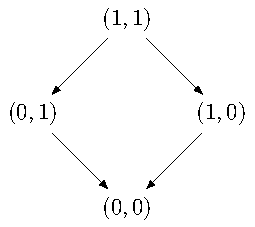
\includegraphics[scale = 0.8]{fig0}
            \caption{Одностоковая ориентация двумерного куба $G(\EE_2^2)$}\label{fig:cube2}
        }
    \end{figure}


    \begin{figure}[ht] % Рисунок
        \centerfloat{
            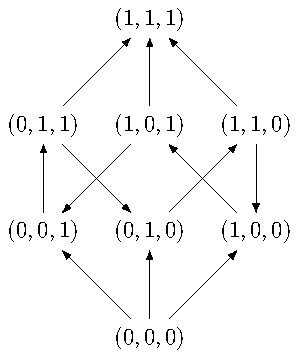
\includegraphics[scale = 0.8]{fig1}
            \caption{Одностоковая ориентация трехмерного куба $G(\EE_2^3)$}\label{fig:cube3}
        }
    \end{figure}

    \begin{definition}
        Пусть задано семейство булевых функций $\ff_n$ размера $n$, в котором функция $f_i$ не зависит существенно от $x_i$, $1 \le i \le n$.
        Тогда семейство $\ff_n$ индуцирует на $G(\EE_2^n)$ ориентацию ребер следующим образом.
        Пусть $(\uu, \vv)$~--- смежные вершины в $G(\EE_2^n)$, различающиеся в $i$-м бите. 
        Рассмотрим значение $i$-й функции семейства $\ff_n$ на этих двух наборах. 
        Поскольку $f_i$ не зависит существенно от одноименной переменной $x_i$, то $f_i(\uu) = f_i(\vv)$. 
        Если $f_i(\uu) = u_i$, то ребро ориентируется от $\vv$ к $\uu$, в противном случае ($f_i(\uu) = v_i$) ребро ориентируется от $\uu$ к $\vv$.
    \end{definition}

    \begin{definition}
        Полученный выше ориентированный граф (граф $G(\EE_2^n)$ с дополнительно индуцированной семейством $\ff_n$ ориентацией ребер) называется асинхронным графом семейства (или асинхронной булевой сетью) $\ff_n$ и обозначается $\Gamma_{\ff_n}$.
    \end{definition}

    \begin{remark}
    \label{rem:fixpt_uso}
        Нетрудно заметить, что вершина $\yy$ является стоком в графе $\Gamma_{\ff_n}$ тогда и только тогда, когда $\yy$~---~неподвижная точка отображения $\ff_n \colon \EE_2^n \to \EE_2^n$.
        Действительно, $\ff(\yy) = \yy$ тогда и только тогда, когда $f_i(\yy) = y_i$ для каждого $i = 1, \ldots, n$, что, в свою очередь, равносильно тому, что $\yy$ является стоком в описанном графе.
    \end{remark}

    \begin{remark}
        Соответствие между семействами $\ff = (f_1, \ldots, f_n)$ булевых функций (где $f_i$ не зависит существенно от $x_i$) и асинхронными графами семейств $\Gamma_{\ff}$ является взаимно-однозначным.
        \begin{enumerate}
            \item По семейству однозначно задается (указанным выше способом) ориентация на графе булева куба $G(\EE_2^n)$.
            \item По ориентированному графу булева куба $\Gamma_{\ff}$ можно восстановить значение всех функций семейства на любом $\xx \in \EE_2^n$: рассмотрим вершину с меткой $\xx$ и все смежные с ней ребра.
            Если $i$-е ребро (ребро, ведущее из вершины $\xx$ в вершину, отличную от $\xx$ в $i$-й координате) выходит из $\xx$, то $f_i(\xx) = \overline{x_i}$, иначе $f_i(\xx) = x_i$.
            В полученном семействе $f_i$ не зависит существенно от $x_i$, поскольку ни одно ребро не ориентировано в две стороны.
        \end{enumerate}
    \end{remark}

\subsection{Неподвижные точки правильных семейств}
\label{sec:boolean_fixpt}
    
    \begin{lemma}[{\cite[лемма~2]{pdm20}}]
    \label{lemma:fixpt}
        У правильного семейства булевых функций всегда существует единственная неподвижная точка.
    \end{lemma}

    \begin{proof}
        Будем вести доказательство индукцией по размеру правильного семейства. 
        Булевы семейства размера $n = 1$~--- это константы $a \in \EE_2^n$, для них утверждение тривиально выполнено.

        Рассмотрим семейство $\ff_n$ размера $n \ge 2$.
        Рассмотрим его проекции $\proj^0_n(\ff_n)$ и $\proj^1_n(\ff_n)$, которые также являются правильными семействами (утверждение~\ref{thm:proj}).
        По предположению индукции для указанных проекций в каждом подкубе существует единственная неподвижная точка:
        \[
            \alpha = (\alpha_1, \ldots \alpha_{n-1}), \;
            \beta = (\beta_1, \ldots \beta_{n-1}),
        \]
        причем точка $\alpha$ соответствует точке $(\alpha, 0)$, лежащей в подкубе с последней координатой $x_n = 0$, а точка $\beta$~--- точке $(\beta, 1)$, лежащей в подкубе с последней координатой $x_n = 1$.
        По определению неподвижных точек выполнены равенства:
        \begin{multline*}
            f_1(\alpha, 0) = \alpha_1, \ldots, f_{n-1}(\alpha, 0) = \alpha_{n-1}, \\
            f_1(\beta, 1) = \beta_1, \ldots, f_{n-1}(\beta, 1) = \beta_{n-1}.
        \end{multline*}
        Рассмотрим значения $f_n(\alpha, 0)$ и $f_n(\beta, 1)$. 
        Так как семейство $\ff_n = (f_1, \ldots, f_n)$~--- правильное, то найдется либо индекс $j \in \{1, \ldots n-1\}$, такой что $\alpha_j \ne \beta_j$, $f_j(\alpha) = f_j(\beta)$, либо $j = n$, и $f_n(\alpha, 0) = f_n(\beta, 1)$.
        Из приведенных выше рассуждений видно, что случай $j < n$ не может выполняться. 
        Следовательно, если $f_j(\alpha) = 0$, то единственной неподвижной точкой всего семейства является $(\alpha, 0)$, иначе такой точкой является точка $(\beta, 1)$.
    \end{proof}

    Следующая теорема устанавливает взаимно-однозначное соответствие между правильными семействами булевых функций размера $n$ и \mbox{$\uso$-ориентациями} булевых кубов размерности $n$.
    \begin{theorem}[{\cite[теорема~2]{pdm20}}]
        Граф семейства $\Gamma_{\ff}$ является одностоковой ориентацией булева куба $\EE_n$ тогда и только тогда, когда $\ff$~--- правильное семейство.
    \end{theorem}

    \begin{proof}
        Как было отмечено выше, стоки в графе $\Gamma_{\ff}$ соответствуют неподвижным точкам ограничения отображения $\ff$ на соответствующий подкуб куба $\EE_n$. 

        Пусть $\ff_n$~---~правильное булево семейство. 
        Тогда по утверждению~\ref{thm:proj} любая проекция семейства $\ff$ на любой подкуб $\EE_n$ также является правильным семейством. 
        По лемме~\ref{lemma:fixpt} такое ограничение имеет единственную неподвижную точку в данном подкубе, т.е. данный подкуб имеет единственный сток. 
        Следовательно, граф $\Gamma_{\ff}$ для правильного семейства $\ff$ является одностоковой ориентацией. 

        Докажем утверждение в обратную сторону. 
        Пусть $\Gamma_{\ff}$~--- одностоковая ориентация. 
        Покажем по индукции, что в этом случае $F$ является правильным семейством. 

        \textbf{База индукции:} при $n = 1$ нетрудно убедиться, что существует ровно две одностоковые ориентации на двух вершинах, соответствующие константным (а значит, правильным) семействам размера 1:
        \begin{equation*}
            \ff^0 = 
            \begin{bmatrix}
                0
            \end{bmatrix}, \quad
            \ff^1 = 
            \begin{bmatrix}
                1
            \end{bmatrix}.
        \end{equation*}

        \textbf{Индуктивный переход:} пусть $\alpha \ne \beta$, где $\alpha, \beta \in \EE_2^n$.
        По определению правильного семейства мы должны показать, что тогда существует индекс $i$, такой что $\alpha_i \ne \beta_i$, но $f_i(\alpha) = f_i(\beta)$.
        Если найдется индекс $k$, такой что $\alpha_k = \beta_k$, то задача может быть сведена к задаче меньшей размерности: рассмотрим проекцию на подкуб $x_k = \alpha_k$ и используем индуктивное предположение.
        
        Следовательно, можем считать, что $\alpha_k \ne \beta_k$, $1 \le k \le n$. 
        Дополнительно мы можем считать, что $\alpha$~--- сток, то есть $f_k(\alpha) = \alpha_k$, $1 \le k \le n$. 
        Если это не так, то мы можем перейти к новому семейству $g_k(\xx) = f_k(\xx) \oplus 1$, таким образом изменив направление всех ребер между подкубами ${x_k = 0}$ и $x_k = 1$. 
        Данная смена направлений ребер не разрушает свойство ориентации быть одностоковой. 
        В силу теоремы~\ref{thm:outer_shift} указанное преобразование не нарушает правильность семейства.
        Таким образом, можно без ограничения общности считать, что вершина $\alpha$ является стоком.

        Но в таком случае если $f_k(\alpha) \ne f_k(\beta)$, $1 \le k \le n$, то мы имеем $f_k(\beta) = \beta_k$, $1 \le k \le n$, то есть вершина $\beta$ также является стоком, что противоречит одностоковости. 
        Следовательно, должен найтись какой-либо индекс $k$, для которого $f_k(\alpha) = f_k(\beta)$, что и требовалось доказать.
    \end{proof}

    Таким образом, учитывая то, что стокам в $\uso$-ориентациях соответствуют неподвижные точки семейства (см. замечание~\ref{rem:fixpt_uso}), был получен следующий критерий правильности семейства (см. также раздел~\ref{sec:hupfnet}).
    \begin{corollary}
        Семейство булевых функций $\ff_n$ правильно тогда и только тогда, когда каждое подсемейство семейства $\ff_n$ (в том числе и само исходное семейство) имеет единственную неподвижную точку. 
    \end{corollary}
    В работе~\cite{fpm23} (см. теорему~2) было показано, что данный критерий нельзя напрямую распространить с булева случая на случай $k$-значной логики, где $k \ge 3$.
    Более точно, было показано, что если семейство $\ff_n$ в $k$-значной логике является правильным, то у него и всех его проекций существует единственная неподвижная точка, однако обратное утверждение неверно: так, например, для семейства
    \begin{equation*}
        \begin{bmatrix}
            f_1(x_1, x_2) \\
            f_2(x_1, x_2)
        \end{bmatrix} = 
        \begin{bmatrix}
            2x_2 \\
            x_1
        \end{bmatrix}
    \end{equation*}
    выполняется свойство единственности неподвижной точки для всех возможных подсемейств, однако семейство не является правильным (см.~\cite{galatenko21criterion}).
    Обобщение критерия может быть сформулировано в терминах перекодировок исходного семейства (см. раздел~\ref{sec:reencoding} и утверждение~\ref{thm:reencoding_properness}).

\subsection{Оценки на число правильных булевых семейств}

    Полученное выше соответствие между $\uso$-ориентациями и правильными семействами булевых функций позволяет получить оценку на число правильных семейств булевых функций размера $n$.
    Обозначим через $T_k(n)$ количество правильных семейств в $k$-значной логике размера $n$ (если $k = 2$, то индекс $k$ будем опускать).

    \begin{corollary}[{\cite[лемма~6.10]{USOphd}}]
    \label{uso:lowerbound}
        Выполнение следующее неравенство 
        \[
            T(n) \ge 4 \left( T(n-1) \right)^2.
        \]
    \end{corollary}
    Отметим, что более слабая оценка вида $T(n) \ge 2 \left( T(n-1) \right)^2$, или, более общо, 
    \[
        T_k(n) \ge k \cdot \left( T_k(n-1) \right)^k
    \] 
    для случая $k$-значной логики может быть получена за счет явных конструкций построения новых правильных семейств из старых (см., например,~\cite[теорема~2]{galatenko20algo}).

    % TODO: неужели не получается обобщить на k-значную логику?

    % Результат из следствия~\ref{uso:lowerbound} можно усилить на случай $k$-значной логики.
    % Доказательство является адаптацией рассуждений из работы~\cite{USOphd} на язык правильных семейств.
    % \begin{corollary}
    % \label{uso:klowerbound}
    %     Обозначим за $T_k(n)$ количество правильных семейств $k$-значной логики размера $n$. 
    %     Тогда $T_k(n+1) \ge k^2 (T_k(n))^k$. 
    % \end{corollary}

    % \begin{proof}
    %     Рассмотрим процедуру построения семейства размера $n+1$ из семейств размера $n$.
    %     Для начала построим $k$ <<рекурсивных>> ориентаций: пусть $\ff^i_{n}$, $0 \le i \le k-1$~--- $k$ правильных семейств размера $n$.

    %     Зададим функцию $f_{n+1}(x_1, \ldots, x_{n+1}) \equiv a$, где $a \in \EE_k$~--- произвольный элемент, и зададим семейство размера $n+1$ как:
    %     \[
    %         \ff_{n+1}(x_1, \ldots, x_{n+1}) = 
    %         \begin{bmatrix}
    %             \bigvee_{0 \le j \le k-1} \II_{x_{n+1}}(j) \wedge \ff^i_{n}(x_1, \ldots, x_n) \\
    %             a
    %         \end{bmatrix}.
    %     \]
    %     Заметим, что проекции $\ff_{n+1}$ вида $x_{n+1} \gets b$, $0 \le b \le k-1$ имеют вид:
    %     \[
    %         \proj^{b}_{n+1} \left( \ff_{n+1} \right) = \ff^b_n(x_1, \ldots, x_n).
    %     \]
    %     Указанным образом можно получить $k$ различных правильных семейств для каждой фиксации набора правильных семейств $\ff^j_n$, $0 \le j \le n-1$, а значит, общее число получаемых таким образом семейств размера $n+1$ равно 
    %     \[
    %         k \cdot (T_k(n))^k.
    %     \] 

    %     Теперь рассмотрим построение не-рекурсивных семейств.
    %     Возьмем произвольные точки $v_1, \ldots, v_k \in \EE_k^n$ и произвольное правильное семейства $\ff^0$ размера $n$.
    %     Рассмотрим множества правильных семейств, которые в заданной точке $\xx$ принимают заданное значение $\vv$:
    %     \[
    %         V(\xx, \vv) = \{\ff_n \mid \ff_n(\xx) = \vv \}.
    %     \]
    %     Заметим, что множества $V(\xx, \vv)$ не пересекаются и равномощны для разных значений $\vv$, поскольку множество $V(\xx, \ww)$, $\ww \ne \vv$ можно получить сдвигом всех функций $V(\xx, \vv)$ на вектор значений $\ww - \vv$, а значит:
    %     \[
    %         V(\xx, \vv) = \frac{T_k(n)}{k^n}.
    %     \]
    %     По выбранному семейству $\ff^0$ выберем семейства $\ff^1, \ldots, \ff^k$ таким образом, что $\ff^j(\vv_j) = \ff^0(\vv_j)$; другими словами:
    %     \[
    %         \ff^j \in V(\vv_j, \ff^0(\vv_j)).
    %     \]
    %     Построим семейство размера $n+1$ следующим образом:
    %     \[
    %         \ff_{n+1}(x_1, \ldots, x_{n+1}) = 
    %         \begin{bmatrix}
    %             \bigvee_{0 \le j \le k-1} \II_{x_{n+1}}(j) \wedge \ff^i(x_1, \ldots, x_n) \\
    %             f_{n+1}(x_1, \ldots, x_n)
    %         \end{bmatrix}.
    %     \]
    %     Поскольку проекции семейства $\ff_{n+1}$ различны при различных $\ff^0, \ldots, \ff^k$, то при каждой фиксации последних мы будем получать некоторое отличное от предыдущих построенных семейство размера $n+1$.
    %     Зададим функцию $f_{n+1}$ следующим образом:
    %     \begin{itemize}
    %         \item если $\xx_0 \not \in \{\vv_1, \ldots, \vv_k\}$, то положить $f_{n+1}(\xx_0) = a$,
    %         \item положить $f_{n+1}(\vv_j) = a_j$.
    %     \end{itemize}
    %     Полученное таким образом семейство будет правильным при любом выборе $a$ и $a_j$:
    %     \begin{itemize}
    %         \item если два набора $\xx$ и $\yy$ отличаются в $n+1$-й координате 
    %     \end{itemize}



    % \end{proof}

    

    \begin{proposition}[{\cite[теорема~1]{numberUSO}}]
    \label{thm:num_of_proper}
        Cуществуют константы $B \ge A > 0$, такие что для $n \ge 2$ выполняются неравенства:
        \[ 
            n^{A \cdot 2^n} \le T(n) \le n^{B \cdot 2^n}.
        \]
    \end{proposition}

    В частности, из этого результата следует, что доля булевых правильных семейств даже среди булевых семейств, для которых $f_i$ не зависит существенно от $x_i$ (необходимое условие правильности, см. замечание~\ref{rem:essential_general}), является экспоненциально малой.

    Также, используя полученную выше оценку, можно показать, что число треугольных семейств среди правильных есть $o(1)$ при стремлении размера семейства $n \to \infty$, а именно, что доля треугольных семейств среди правильных убывает со скоростью ${n^{-D \cdot 2^n}}$, где $D > 0$ (т.е. экспоненциально мала).

    \begin{theorem}[{\cite[теорема~6]{dm21}}]
    \label{thm:triangle}
        Обозначим через $\Delta(n)$ количество булевых треугольных семейств размера $n$.
        Тогда:
        \[
            \frac{\Delta(n)}{T(n)} = o \left(\frac{1}{n^{D \cdot 2^n}} \right)
            \text{ при } n \to \infty
        \]
        для некоторого $D > 0$.
    \end{theorem}

    Докажем несколько вспомогательных утверждения (верхнюю и нижнюю оценки на число $\Delta(n)$, а также техническую лемму, необходимую для оценки).

    \begin{lemma}[{\cite[лемма~3]{dm21}}]
    \label{lemma:seriessum}
        Выполнено неравенство:
        \[
            \sum_{k=2}^{\infty} \frac{k}{2^{2^{k-1}}} < 0.705.
        \]
    \end{lemma}

    \begin{proof}
        С помощью компьютерных вычислений можно убедиться, что: 
        \[
            \sum_{k=2}^{10} \frac{k}{2^{2^{k-1}}} < 0.704.
        \]
        Остаток ряда можно оценить следующим образом:
        \[
            \sum_{k=11}^{\infty} \frac{k}{2^{2^{k-1}}} < \sum_{k=11}^{\infty} \frac{1}{2^k} < 0.001,
        \]
        поскольку для каждого члена ряда выполнено неравенство (при $k>4$):
        \[
            \frac{k}{2^{2^{k-1}}} < \frac{1}{2^k} 
            \Leftrightarrow
            k \cdot 2^k < 2^{2^{k-1}}.
        \]
    \end{proof}


    \begin{lemma}[{\cite[лемма~1]{dm21}}]
        \label{lemma:num_triangle}
        Выполнено следующее неравенство:
        \[
            \Delta(n) \le n! \cdot 2^{2^n - 1}.
        \]
    \end{lemma}

    \begin{proof}
        Зафиксируем подстановку $\sigma \in \SSS_n$ и оценим сверху число булевых функций, которые могут стоять на позиции $\sigma(m)$ значением $2^{2^{m-1}}$, поскольку функция с номером $\sigma(m)$ зависит существенно не более чем от $m-1$ переменной.
        В таком случае общее число треугольных семейств не превышает:
        \[
            \Delta(n) \le n! \cdot 2^{2^0} \cdot 2^{2^1} \cdot \ldots \cdot 2^{2^{n-1}} = n! \cdot 2^{2^n-1}.
        \]
    \end{proof}

    Заметим, что некоторые семейства при такой оценке могли быть подсчитаны более одного раза. 
    Тем не менее, оценка является достаточно точной, а именно, выполняется следующее утверждение.

    \begin{lemma}[{\cite[лемма~2]{dm21}}]
        \label{lem:lower_bound}
        Выполнено следующее неравенство:
        \[
            \Delta(n) \ge 0.145 \cdot n! \cdot 2^{2^n-1}.
        \]
    \end{lemma}

    \begin{proof}
        Через $e(n)$ обозначим число $n$-местных булевых функций, существенно зависящих от всех $n$ переменных.
        Тогда количество треугольных семейств может быть оценено снизу значением
        \[
            \Delta(n) \ge n! \cdot e(0) \cdot e(1) \cdot \ldots \cdot e(n-1),
        \]
        поскольку в данном случае мы подсчитываем число треугольных семейств, в которых после упорядочивания первая функция существенно зависит ровно от $0$ переменных, вторая функция зависит существенно ровно от одной переменной $x_{\sigma(1)}$, и так далее. 
        При этом при различных $\sigma$ мы получаем заведомо различные семейства. 
        Необходимо оценить снизу полученное произведение.

        Можно оценить число $e(n)$ снизу согласно неравенству Бонферрони (см.~\cite[раздел~1.3]{Zuev}):
        \[
            e(n) \ge 2^{2^n} - n \cdot 2^{2^{n-1}}.
        \]
        Данная оценка получается из следующих соображений: из множества всех булевых функций от $n$ переменных $x_1, \ldots, x_n$ вычтем все функции, которые зависят только от $n-1$ выбранной переменной (имеется $n$ способов зафиксировать одну переменную, от которой не будет зависеть функция).

        При этом данная оценка является оценкой снизу, поскольку некоторые функции учитываются более одного раза в вычитаемом (например, функции, не зависящие одновременно от двух переменных).

        Таким образом,
        \begin{multline*}
            \frac{\Delta(n)}{n! \cdot 2^{2^0} \cdot 2^{2^1} \cdot \ldots \cdot 2^{2^{n-1}}} \ge 
            \frac{e(0)}{2^{2^0}} \times \ldots \times \frac{e(n-1)}{2^{2^{n-1}}} \ge \\
            \ge 1 \cdot \left( 1 - \frac{1}{2^{2^0}} \right) \cdot 
            \left( 1 - \frac{2}{2^{2^1}} \right) \times 
            \ldots \times 
            \left( 1 - \frac{n-1}{2^{2^{n-2}}} \right) \ge \\
            \ge \frac{1}{2} \cdot \left( 1 - \left( \frac{2}{2^{2^1}} + \ldots + \frac{n-1}{2^{2^{n-2}}} \right) \right) \ge \\
            \ge \frac{1}{2} \left( 1 - \sum_{k=2}^{\infty} \frac{k}{2^{2^{k-1}}} \right).
        \end{multline*}

        Для завершения доказательства леммы~\ref{lem:lower_bound} остается воспользоваться оценкой сверху для ряда $\sum_{k=2}^{\infty} \frac{k}{2^{2^{k-1}}}$.
        Используя лемму~\ref{lemma:seriessum}, получим:
        \[
            \frac{1}{2} \left( 1 - \sum_{k=2}^{\infty} \frac{k}{2^{2^{k-1}}} \right) \ge \frac{1}{2}(1 - 0.705) = 0.1475,
        \]
        откуда следует утверждение леммы \ref{lem:lower_bound}.
    \end{proof}

    Таким образом, можно утверждать, что при $n \to \infty$ имеется оценка:
    \[
        \Delta(n) = \Theta \left( n! \cdot 2^{2^n-1} \right).
    \]
    Перейдем к доказательству теоремы~\ref{thm:triangle}.

    \begin{proof}
        Используя нижнюю оценку из утверждения~\ref{thm:num_of_proper} и формулу Стирлинга (см., например,~\cite[часть~II, параграф~4]{yablonski}), можно оценить долю треугольных семейств среди правильных:

        \begin{multline*}
            \frac{\Delta(n)}{T(n)} \le \frac{n! \cdot 2^{2^n - 1}}{n^{A\cdot 2^n}} \sim
            \frac{n^n \cdot 2^{2^n-1} \cdot \sqrt{2\pi n}}{e^n \cdot n^{A\cdot 2^n}} = \\
            = \Theta \left(
                \frac{2^{(n+\frac{1}{2})\log n} \cdot 2^{2^n}}{2^{n \log e} \cdot 2^{A \cdot 2^n \log n}}
            \right) = \\ 
            = \Theta \left(
                2^{2^n (1 - A \log n)} \cdot 2^{n \cdot (\log n - \log e + \frac{\log n}{2n})}
            \right) = \\
            = o \left( 2^{-(A - \varepsilon) \cdot 2^n \log n} \right)
            \text{ при } n \to \infty
        \end{multline*}
        для любого $\varepsilon > 0$.
        Для того, чтобы удостовериться в этом, заметим, что 
        \[
            \frac{2^{2^n (1 - A \log n)} \cdot 2^{n \cdot (\log n - \log e + \frac{\log n}{2n})}}{2^{-(A - \varepsilon) \cdot 2^n \log n}} =
            2^{-\varepsilon \cdot 2^n \log n \cdot (1 + o(1))},
        \]
        и при $n \to \infty$ показатель стремится к $-\infty$.

        Отсюда следует утверждение теоремы~\ref{thm:triangle} для $D = A  - \varepsilon$ для любого фиксированного $0 < \varepsilon < A$.
    \end{proof}

    Из доказанной теоремы следует, что булевы треугольные семейства размера $n$ образуют лишь экспоненциально малую часть от всех правильных семейств булевых функций размера $n$.

\subsection{Рекурсивно треугольные семейства}

    Еще одним примером \textquote{переноса} результатов с геометрического языка $\uso$-ориентаций на алгебраический язык правильных семейств является понятие рекурсивно треугольного семейства.
    В работе~\cite{gao2020new} вводится понятие рекурсивной ориентации булева куба.
    Рекурсивная ориентация булева $n$-мерного куба $G(\EE_2^n)$ задается следующим характеристическим свойством: найдется такая координата $x_i$, вдоль которой все ребра ориентированы в одном направлении, и ориентация на каждом из подкубов $x_i = 0$ и $x_i = 1$ размерности $(n-1)$ также является рекурсивной.
    Мы можем обобщить указанную конструкцию, перенеся ее на алгебраический язык правильных семейств следующим образом.

    \begin{definition}
    \label{def:rectriangle}
        Назовем семейство $\ff_n$, заданное на $Q^n$, рекурсивно треугольным, если существует координата $i$, такая что $f_i = q \in Q$ (константа), и каждое из семейств вида $\proj^a_i(\ff_n)$, где $a$ пробегают все множество $Q$, также является рекурсивно треугольным.
    \end{definition}

    \begin{remark}
        Треугольные семейства являются частным случаем рекурсивно треугольных: треугольные семейства являются такими рекурсивно треугольными, что каждая из проекций $\proj^a_i(f_n)$ постоянна вдоль одного и того же направления~$j$.
    \end{remark}

    Класс рекурсивно треугольных семейств вкладывается в класс локально треугольных семейств (см. определение~\ref{def:localtriangle}).
    Как будет показано далее, локально треугольные семейства являются правильными, а следовательно, и рекурсивно треугольные семейства также являются правильными.

    Введем обозначение $\Delta^{\rec}_k(n)$ для числа рекурсивно треугольных семейств $k$-значной логики размера $n$.
    
    \begin{lemma}
        Для числа рекурсивно треугольных семейств справедлива формула:
        \[
            \Delta^{\rec}_{k}(n) = \sum_{j=1}^{n} (-1)^{j+1} \cdot k^j \cdot {n \choose j} \left( \Delta^{\rec}_{k}(n-j) \right)^{k^j},
        \]
        где $\Delta^{\rec}_{k}(0) = 1$, $k = \lvert Q \rvert$.
    \end{lemma}

    \begin{proof}
        Утверждение следует напрямую из формулы включений-исключений (см., например,~\cite[часть~II, параграф~3]{yablonski}).
        Существует ${n \choose j}$ способов выбрать $j$ \textquote{фиктивных направлений}, для которых $f_{\ell} = const$, и $k^j$ способов зафиксировать значения $j$ фиктивных функций.
        Каждая из проекций должна образовывать рекурсивно треугольное семейство размера $n-j$, и различные рекурсивно треугольные семейства в проекциях могут выбираться независимо друг от друга, что дает итоговый вклад $\left( \Delta^{\rec}_{k}(n-j) \right)^{k^j}$.
    \end{proof}

    \begin{remark}
        Для $k=2$ число рекурсивно треугольных семейств размера $n$ совпадает с числом рекурсивных ориентаций куба $G(\EE_2^n)$~\cite[A141770]{oeis}.
    \end{remark}

    \begin{theorem}
        Доля булевых рекурсивно треугольных семейств размера $n$ в классе всех булевых правильных семейств размера $n$ стремится к 0 при $n \to \infty$. 
    \end{theorem}

    \begin{proof}
        Для числа рекурсивно треугольных семейств справедливо неравенство:
        \[
            \Delta^{\rec}_{k}(n) \le n \cdot k \cdot \left( \Delta^{\rec}(n-1) \right)^k.
        \]
        Применяя неравенство рекурсивно и используя равенство $\Delta^{\rec}_{k}(0) = 1$, можно получить оценку:
        \[
            \Delta^{\rec}_{k}(n) \le \left(n^{k^0} \cdot (n-1)^{k^1} \cdot (n-2)^{k^2} \times \ldots \times (n - (n-1))^{k^{n-1}}\right) \cdot k^{\frac{k^n - 1}{k-1}}.
        \]

        Обозначим через $S(n, k)$ число вида:
        \[
            S(n, k) = \prod_{i=0}^{n-1} \left( n - i \right)^{k^i},
        \]
        тогда согласно полученному неравенству имеем 
        \[
            \Delta^{\rec}_{k}(n) \le S(n, k) \cdot k^{\frac{k^n - 1}{k-1}}.
        \]

        Для $S(n, 2)$ верна следующая асимптотика при $n \to \infty$~\cite[раздел~6.10]{finch2003mathematical}:
        \begin{gather*}
            S(n, 2) \sim \frac{s^{2^n}}{n}, \\
            s = \sqrt{1 \cdot \sqrt{2 \cdot \sqrt{3 \cdot \ldots}}} \approx 1.661688.
        \end{gather*}
        Таким образом, для величины $\Delta^{\rec}_{2}(n)$ справедливо асимптотическое неравенство:
        \[
            \Delta^{\rec}_{2}(n) \lesssim \frac{(2s)^{2^n}}{2n},
        \]
        а для доли рекурсивно треугольных с учетом неравенства на число правильных булевых семейств размера $n$ (см. утверждение~\ref{thm:num_of_proper}) выполняется 
        \[
            \frac{\Delta^{\rec}_{2}(n)}{T(n)} \lesssim \frac{1}{2n} \cdot \left( \frac{2s}{n} \right)^{2^n}.
        \]
        Полученная величина стремится к 0 при $n \to \infty$.
    \end{proof}

    \begin{remark}
        В общем случае для чисел $S(n,k)$ верна асимптотика~\cite{xu2019asymptotic}:
        \[
            S(n, k) \sim \frac{\left(A_k\right)^{k^n}}{n^{\frac{1}{1-k}}},
        \]
        где $A_k$~--- некоторая константа, зависящая только от $k$.
    \end{remark}


%%%%%%%%%%%%%%%%%%%%%%%%%%%%%%%%%%%%%%%%%%%%%%%%%%%%%%%%%


\section{Булевы сети с наследственно единственной неподвижной точкой}
\label{sec:hupfnet}

    Введенное ранее понятие асинхронного графа семейства $\Gamma_{\ff}$ (асинхронной булевой сети) имеет и другую сферу приложения.
    А именно, подобные сети рассматриваются в контексте математической биологии~\cite{kaufman69, thomas73, de2002modeling} как аппарат для изучения экспрессии генов~\cite{thomas1991regulatory}.
    В указанном контексте особо интересны неподвижные точки асинхронной булевой сети~\cite{richard2015fixed, ruet2015asynchronous, ruet2016local}, которые соответствуют устойчивым паттернам экспрессии генов~\cite{richard2015fixed}.

    Оказывается, что правильные семейства булевых функций задают такие асинхронные булевы сети, что в каждой порожденной подсети (которые соответствуют рассмотрению проекции подсемейства) существует единственная неподвижная точка (такой объект обычно называется \textquote{асинхронной булевой сетью с наследственно единственной неподвижной точкой}, или сокращенно $\hupf$-сетью, от англ. hereditarily unique fixed point network).
    Несложно видеть, что в $\hupf$-семействе каждая функция $f_i$ не может зависеть существенно от одноименной переменной $x_i$ (в противном случае соотвествующая проекция имела бы 0 или 2 неподвижные точки).

    Для исходного правильного семейства неподвижная точка существует и единственна по лемме~\ref{lemma:fixpt}, и при этом каждая проекция правильного семейства также является правильным семейством (см. утверждение~\ref{thm:proj}), и, в свою очередь, также имеет единственную неподвижную точку.
    Таким образом, верна следующая теорема.
    \begin{theorem}
        \label{thm:proper_hupf}
        Булевы правильные семейства находятся во взаимно-однозначном соответствии с $\hupf$-сетями.
    \end{theorem}

    С помощью полученного естественного соответствия мы можем переносить результаты из области $\hupf$-сетей на \textquote{язык} правильных семейств (и наоборот).
    В этом разделе мы рассмотрим некоторые из подобных результатов.


\subsection{Локальные графы взаимодействий и локально треугольные семейства}

    Пусть $f \colon Q^n \to Q$~--- функция на $Q^n$.
    \begin{definition}
        Введем частную производную $\dd_i f(\xx) \in \{0, 1\}$ в точке $\xx$:
        \[
            \dd_i \ff(\xx) = 
            \begin{cases}
                1, & \text{если существует $q$, т.ч.} \\
                & \ff_n(x_1, \ldots, x_{i-1}, q, x_{i+1}, \ldots, x_n) \ne \ff(x_1, \ldots, x_{i-1}, x_i, x_{i+1}, \ldots, x_n),\\
                0, & \text{ в противном случае.} \\
            \end{cases}
        \]
    \end{definition}

    В работе~\cite{shih2005combinatorial} было введено понятие локального графа взаимодействия для семейства $\ff$ в точке $\xx$.
    По сути, это понятие определяет \textquote{локализованный} в точке $\xx$ граф существенной зависимости семейства $\ff$, а именно, он показывает, как локальные изменения аргумента в точке $\xx$ влияют на поведение семейства.

    \begin{definition}
        Определим локальный граф взаимодействий $G_{\ff}(\xx)$ семейства $\ff$ в точке $\xx$ как ориентированный граф на множестве вершин $V = {1, 2, \ldots, n}$, вершины с номерами $j$ и $i$ соединяются ориентированным ребром $j \to i$ тогда и только тогда, когда $\dd_i f_j(x) \ne 0$.
    \end{definition}

    \begin{remark}
        Можно также определить глобальный граф взаимодействий $G_{\ff}$ семейства $\ff$ как ориентированный граф на множестве вершин $V = {1, 2, \ldots, n}$, вершины с номерами $j$ и $i$ соединяются ориентированным ребром $j \to i$ тогда и только тогда, когда существует точка $\xx$, для которой $\dd_i f_j(\xx) \ne 0$.

        Иными словами, в глобальном графе взаимодействий присутствует ребро $j \to i$ тогда и только тогда, когда $f_j$ существенно зависит от $x_i$.
        Следовательно, глобальный граф взаимодействий совпадает с (уже введенным) графом существенной зависимости семейства $G_{\ff}$ (см. определение~\ref{def:essgraph}).
        Заметим также, что глобальный граф взаимодействий $G_{\ff}$ представляет собой объединение локальных графов взаимодействий $G_{\ff}(\xx)$ по всем точкам $\xx$.
    \end{remark}

    В работе~\cite{robert1980iterations} было показано, что если глобальный граф взаимодействия $G_{\ff}$ булева семейства $\ff$ является ациклическим, то семейство $\ff$ задает $\hupf$-сеть.
    По сути, было показано, что треугольные семейства являются правильными.
    Обобщение указанного результата приведено в работе~\cite{shih2005combinatorial}, где было показано, что если локальный граф взаимодействия булева семейства $\ff$ для каждой точки $\xx$ является ациклическим, то семейство задает $\hupf$-сеть.
    Мы можем обобщить указанное наблюдение на любые (не только булевы) семейства $\ff$ (см. теорему~\ref{thm:localproper}).
    Дадим предварительные определения.

    \begin{definition}
    \label{def:localtriangle}
        Назовем семейство $\ff$, заданное на $Q^n$, локально треугольным в точке $\xx$, если существует такая согласованная перестановка семейства $\sigma$, что после ее применения мы получим семейство $\gf$ со свойством
        \[
            \dd_i g_j(\xx) = 0, \quad 1 \le j \le i \le n.
        \]
        Назовем семейство $\ff$ локально треугольным, если оно является локально треугольным в каждой точке $\xx \in Q^n$.
    \end{definition}

    \begin{lemma}
        Семейство $\ff$ локально треугольно в точке $\xx$ тогда и только тогда, когда $G_{\ff}(\xx)$ задает направленный ациклический граф.
    \end{lemma}

    \begin{proof}
        Перейдем к согласованной перестановке семейства $\ff$~--- семейству $\gf$.
        Для переставленного семейства $\gf$ первая функция $g_1$ локально постоянна по любому из направлений, функция $g_2$ локально постоянна по направлениям $x_2, \ldots, x_n$, и так далее.
        Это значит, что из вершины с номером $i$ в графе $G_{\gf}(\xx)$ могут выходить ребра только к вершинам с номерами $j < i$.
        Если в графе $G_{\gf}(\xx)$ существует цикл $i_1 \to i_2 \to i_k \to i_1$, то указанное свойство нарушается: достаточно рассмотреть вершину с наибольшим номером в цикле.
        По указанному выше свойству ребра к этой вершине могут идти только от вершин с большими номерами, но все оставшиеся номера в цикле меньше, чем у рассматриваемой вершины.
        Мы пришли к противоречию, которое доказывает, что в графе $G_{\gf}(\xx)$ не может быть направленных циклов.
        Поскольку согласованная перестановка семейства только меняет метки у вершин графа $G_{\ff}(\xx)$, то и в исходном графе не может быть циклов.

        Докажем в обратную сторону: пусть в $G_{\ff}(\xx)$ нет циклов. 
        Тогда существует топологическая сортировка графа $G_{\ff}(\xx)$ (см., например,~\cite[раздел~22.4]{cormen}), т.е. такая перенумерация вершин $\sigma$, что после нее в графе остаются только такие ребра $(i, j) \in E$, для которых $i > j$.
        Если применить $\sigma$ к семейству $\ff$ как согласованную перенумерацию, то функция $f_1$ не будет зависеть существенно в точке $\xx$ ни от какой из переменных, функция $f_{2}$ может зависеть только от $x_1$ и так далее.
        Поскольку это верно для каждой точки $\xx$, то по определению $\ff$ является локально треугольным семейством.
    \end{proof}

    \begin{lemma}
    \label{lemma:localproj}
        Пусть $\ff$~--- локально треугольное семейство, $\gf$~--- некоторая его проекция.
        Тогда $\gf$ также является локально треугольным семейством.
    \end{lemma}

    \begin{proof}
        Без ограничения общности рассмотрим однократную проекцию вида $\gf = \proj^{a}_{i}(\ff)$.
        Тогда граф $G_{\gf}(\xx)$ для точки $\xx = (x_1, \ldots, x_{i-1}, x_{i+1}, \ldots, x_n) \in Q^{n-1}$ совпадает с графом $G_{\ff}((x_1, \ldots, x_{i-1}, a, x_{i+1}, \ldots, x_n))$ с удаленной $i$-й вершиной (и всеми инцидентными ей ребрами).
        При удалении вершины новых циклов появиться не может, а значит, графы $G_{\gf}(\xx)$ остаются ациклическими для каждой точки $\xx$.
        Следовательно, $\gf$ локально треугольно.
    \end{proof}

    \begin{lemma}
    \label{lemma:localantipode}
        Пусть $v_1 \ne y_1, \ldots, v_n \ne y_n$, $\ff_n$ локально треугольное.
        Тогда найдется такой индекс $i$, что $f_i(\vv) = f_i(\yy)$.
    \end{lemma}

    \begin{proof}
        Проведем доказательство индукцией по размеру семейства $n$.
        \textbf{База индукции:} при $n = 1$ локально треугольными семействами размера 1 будут только константы $\ff = \begin{bmatrix} a \end{bmatrix}$, $a \in \EE_k$.

        \textbf{Индуктивный переход:} рассмотрим $n \ge 2$.
        Так как $\ff_n$ локально треугольно в точке $\vv$, то найдется такая координата (без ограничения общности можем предполагать, что $x_n$), что при ее варьировании при остальных фиксированных координатах никакая из функций не поменяется.

        Рассмотрим проекцию вида $\gf = \proj^{y_n}_n(\ff_n)$.
        В таком случае мы переходим к локально треугольному (см. лемму~\ref{lemma:localproj}) семейству $\gf$ размера $n-1$, по предположению индукции найдется индекс $j < n$, такой что 
        \begin{equation*}
            f_j(v_1, \ldots, v_{n-1}, y_n) = g_j(v_1, \ldots, v_{n-1}) = g_j(y_1, \ldots, y_{n-1}) = f_j(y_1, \ldots, y_{n-1}, y_n).
        \end{equation*}
        Но поскольку исходное семейство $\ff_n$ локально постоянно вдоль направления $x_n$ в точке $\vv$, то 
        \[
            f_j(v_1, \ldots, v_{n-1}, v_n) = f_j(v_1, \ldots, v_{n-1}, y_n) = f_j(y_1, \ldots, y_{n-1}, y_n),
        \] 
        что и требовалось доказать.
    \end{proof}

    \begin{theorem}
    \label{thm:localproper}
        Пусть $\ff$~--- заданное на $Q^n$ локально треугольное семейство.
        Тогда $\ff$ является правильным.
    \end{theorem}

    \begin{proof}
        Для любых двух неравных наборов $\xx \ne \yy$, $\xx, \yy \in Q^n$ рассмотрим проекцию $\gf$ исходного семейства $\ff$ на общие координаты.
        Проекция $\gf$ будет локально треугольным семейством по лемме~\ref{lemma:localproj}.
        К семейству $\gf$ можно применить лемму~\ref{lemma:localantipode} и получить индекс $i$, для которого значения функций $g_i$ в рассматриваемой точке совпадут, а значит, для исходного семейства $\ff$ выполняется характеристическое свойство правильности.
    \end{proof}

    \begin{remark}
    \label{ex:loctr}
        Множество булевых локально треугольных семейств шире множества треугольных семейств (см. раздел~\ref{sec:triangle}).
        Так, например, булевы семейства 
        \begin{equation}
            \begin{bmatrix}
                0 \\
                x_1 \oplus x_3 \\
                x_1 \oplus x_2 \oplus x_1 x_2 \\
            \end{bmatrix},
            \begin{bmatrix}
                x_2 x_ 3 x_4 \\
                x_1 \oplus x_1 x_3 \\
                x_2 \oplus x_1 x_2 \oplus x_2 x_4 \oplus x_1 x_2 x_4 \\
                x_1 \oplus x_1 x_2 \oplus x_1 x_3 \oplus x_1 x_2 x_3 \\
            \end{bmatrix}
        \end{equation}
        являются локально треугольными, но не треугольными.
    \end{remark}

    Покажем, что рекурсивно треугольные семейства (см. определение~\ref{def:rectriangle}) являются локально треугольными (а следовательно, правильными).

    \begin{lemma}
        Пусть $\ff_n$~--- рекурсивно треугольное семейство на $Q^n$.
        Тогда $\ff_n$ является локально треугольным семейством.
    \end{lemma}

    \begin{proof}
        Покажем, что для каждой точки $\vv$ граф $G_{\ff}(\vv)$ является ациклическим.
        Для рекурсивно треугольных семейств размера $n = 1$ и $n = 2$ утверждение проверяется напрямую.

        Пусть $\ff_n$~--- рекурсивно треугольное семейство размера $n$.
        По свойству рекурсивной треугольности найдется такой индекс $i$, что $f_i \equiv const$, а следовательно, вершина с номером $i$ в графе $G_{\ff}(\vv)$ является истоком (в нее не входит ребер), т.к. $f_i$ не зависит ни от одного $x_j$ существенным образом.
        Следовательно, вершина $i$ не может входить ни в какой из циклов.

        Рассмотрим какую-либо проекцию $\gf = \proj_i^{a}(\ff)$ и ее локальный граф взаимодействий в точке $\widetilde{\vv} = (v_1, \ldots, v_{i-1}, v_{i+1}, \ldots, v_n)$.
        Граф $G_{\gf}(\widetilde{\vv})$ является подграфом графа $G_{\ff}(\vv)$.
        При этом если в графе $G_{\ff}(\vv)$ был цикл, то он останется хотя бы в одном из $G_{\gf}(\widetilde{\vv})$.
        Но каждое из семейств $\gf$ также является рекурсивно треугольным (меньшего размера), а значит, по предположению индукции, в графах $G_{\gf}(\widetilde{\vv})$ нет циклов.

        Таким образом, исходный граф $G_{\ff}(\vv)$ является ациклическим для любой точки $\vv$.
    \end{proof}


    \begin{remark}
        Свойство рекурсивной треугольности, вообще говоря, слабее свойства локальной треугольности (см., например, семейство размера 4 из замечания~\ref{ex:loctr}: в нём нет константы).

        Фактически, из рекурсивной треугольности следует, что \textit{для всех} графов $G_{\ff}(\vv)$ найдется одна и та же вершина $i$, являющаяся истоком. 
        Для $n = 1, 2, 3$ множества локально треугольных и рекурсивно треугольных семейств совпадают.
        Для $n = 4$ количество локально треугольных семейств $\Delta^{\loc}(4) = 3349488$ превышает число рекурсивно треугольных семейств $\Delta^{\rec}(4) = 3209712$ (см. таблицу~\ref{tab:countfamilies}).
    \end{remark}

    Таким образом, множество локально треугольных семейств шире, чем множество рекурсивно треугольных семейств (и включает его в себя целиком), множество рекурсивно треугольных семейств шире, чем множество треугольных семейств (и включает его в себя целиком).

\subsection{Несамодвойственные проекции}
\label{sec:selfadj}
    
    В настоящем разделе мы сформулируем еще один критерий правильности семейства функций, сформулированного в работе~\cite[раздел~4]{richard2015fixed} для $\hupf$-сетей.
    Для начала дадим предварительные определения.

    Пусть $\ff_n$~--- семейство булевых функций.
    \begin{definition}
        Будем называть отображение $\ff \colon \EE_2^n \to \EE_2^k$ самодвойственным, если для любого набора $\xx \in \EE_2^n$ выполняется свойство $\ff(\overline{\xx}) = \overline{\ff(\xx)}$.
    \end{definition}

    \begin{remark}
        Для $k = 1$ введенное выше определение совпадает со стандартным определением самодвойственной функции (см., например,~\cite[Часть~I, глава~1]{yablonski}).
    \end{remark}

    \begin{remark}
        Свойство самодвойственности сохраняется при всевозможных сдвигах семейства (как внутренних, так и внешних) и при согласованных перестановках.
    \end{remark}

    \begin{theorem}
    \label{thm:self_proper}
        Семейство $\ff_n$ булевых функций правильно тогда и только тогда, когда каждая из его проекций $\proj^{a_1, \ldots, a_k}_{i_1, \ldots, i_k}(\ff)$ не является самодвойственной булевой функцией.
    \end{theorem}

    Утверждение следует из следствия~2 работы~\cite{richard2015fixed}.

%%%%%%%%%%%%%%%%%%%%%%%%%%%%%%%%%%%%%%%%%%%%%%%%%%%%%%%%%%%%%%%
%%%%% ТУТ РЕЗУЛЬТАТЫ ЧАСТИЧНО НЕПРАВИЛЬНЫЕ, НАДО ИСПРАВИТЬ %%%%
%%%%%%%%%%%%%%%%%%%%%%%%%%%%%%%%%%%%%%%%%%%%%%%%%%%%%%%%%%%%%%%



%     \TODO{исправить лемму, она сейчас неправильно доказана}
%     \begin{lemma}
%         \label{lemma:dual}
%         Пусть семейство булевых функций $\gf \colon \EE_2^n \to \EE_2^n$ таково, что найдется набор $\gamma \in \EE_2^n$, для которого выполнено свойство $\gf(\gamma) = \overline{\gf(\overline{\gamma})}$.
%         Тогда существует самодвойственная проекция $\gf$.
%     \end{lemma}

%     \begin{proof}
%         Докажем утверждение индукцией по $n$.
%         Заметим, что мы можем без ограничения общности считать, что $\gf(\gamma) = \gamma = (0, \ldots, 0)$.
%         Этого можно добиться комбинацией внешнего и внутреннего сдвигов.

%         \textbf{База индукции:} при $n = 1$ семейство $\gf$ по условию утверждения имеет вид $\gf(x) = x$ или $\gf(x) = \overline{x}$, а значит, самодвойственно по определению. 
%         В таком случае можно рассмотреть тривиальную проекцию $\mathsf{id}$.

%         \textbf{Индуктивный переход:}
%         Пусть $n \ge 2$.
%         Рассмотрим исходные наборы-антиподы $\gamma = (0, \ldots, 0)$ и $\bar{\gamma} = (1, \ldots, 1)$.
%         Введем обозначение 
%         \[
%             e_i = \left(\underbrace{0, \ldots, 0}_{i-1}, 1, \underbrace{0, \ldots, 0}_{n-i}\right).
%         \]
%         Рассмотрим \textquote{соседние} с нулевым наборы $e_1, \ldots, e_n$.

%         Покажем, что для всех $i$ выполняются условия:
%         \[
%             \gf(e_i) \ne (0, \ldots, 0), \gf(e_i)[i] \ne 1.
%         \]
%         \begin{enumerate}
%             \item Если для какого-то $i$ выполнено $\gf(e_i) = (0, \ldots, 0)$, то мы можем рассмотреть проекцию 
%             \[
%                 \mathcal{H} = \proj_{i}^{1}(\gf),
%             \]
%             для которой выполняются условия: 
%             \begin{itemize}
%                 \item $\mathcal{H}(0, \ldots, 0) = (0, \ldots, 0)$, поскольку $\gf(e_i) = \gf(0, \ldots, 0) = (0, \ldots, 0)$;
%                 \item $\mathcal{H}(1, \ldots, 1) = (1, \ldots, 1)$, поскольку $\gf(1, \ldots, 1) = (1, \ldots, 1)$.
%             \end{itemize}
%             Таким образом, мы перешли к проекции исходного семейства $\gf$ размера $n-1$, которая обладает тем же характеристическим свойством, что и $\gf$, а значит, к нему применимо предположении индукции.
%             \item Если для какого-то $i$ выполнено $\gf(e_i)[i] = 1$, то мы можем рассмотреть проекцию
%             \[
%                 \mathcal{H} = \proj_{1, \ldots, i-1, i+1, \ldots, n}^{0, \ldots, 0}(\gf).
%             \]
%             Мы получим семейство размера 1, для которого $\mathcal{H}(0) = 0$, $\mathcal{H}(1) = 1$, т.е. самодвойственную проекцию размера 1.
%         \end{enumerate}
        
%         Таким образом, при изменении любой координаты в наборе $(0, \ldots, 0)$, меняется хотя бы одно значение функций $g_j$, но значение $g_i$ остается неизменным.

%         Рассмотрим какое-либо фиксированное направление, например, $e_n$.
%         Пусть $d(\gf(0, \ldots, 0), \gf(e_n)) \le n-2$, то есть 
%         \[
%             \gf(e_n) = e_{i_1} \oplus \ldots \oplus e_{i_k}, \quad k \le n-2.
%         \]
%         Тогда рассмотрим проекцию следующего вида:
%         \[
%             \mathcal{H} = \proj_{i_1, \ldots, i_k}^{0 \ldots 0} \left( \proj_{n}^{1} \left( \gf \right) \right).
%         \]
%         Проекция $\mathcal{H}$ является семейством размера $n-k \ge 2$, причем выполняется свойство 
%         \[
%             \mathcal{H}(0, \ldots, 0) = (0, \ldots, 0), \mathcal{H}(1, \ldots, 1) = 
%         \]

%         Рассмотрим множество путей из вершины $\gamma$ в вершину $\bar{gamma}$ в графе булева куба $G(\EE_2^n)$.

%         Пусть существует путь $\gamma \to \bar{\gamma}$ со следующим свойством: существуют две соседние вершины пути $\uu, \vv$, $d(\uu, \vv) = 1$, для которых расстояние Хэмминга между образами удовлетворяет неравенству 
%         \[
%             d(\gf(\uu), \gf(\vv)) > 1.
%         \] 
%         Пусть $\uu$, $\vv$ различаются только в $i$-й координате, а $\gf(\uu)$ и $\gf(\vv)$ различаются дополнительно в координате $j > i$ (такая координата существует, поскольку расстояние Хэмминга между наборами не менее 2, без ограничения общности несовпадающая координата $j > i$).
%         Рассмотрим проекцию семейства $\gf$ на направления $(i, j)$:
%         \[
%             h(x_i, x_j) = \proj_{1, \ldots, i-1, i+1, \ldots, j - 1, j+1, n}^{u_1, \ldots, u_{i-1}, u_{i+1}, \ldots, u_{j - 1}, u_{j+1}, u_n}(\gf).
%         \]
%         Без ограничения общности мы можем считать, что $h(0, 0) = (0, 0)$, $h(1, 0) = (a, 1)$ (исходные наборы различны в одной координате, наборы-образы различаются в $j$-й координате).
%         Если $a = 1$, то рассмотрим проекцию вида $x_i \gets 0$, получим функцию $f(x) = h(x, 0)[1]$, для которой $f(0) = 0$, $f(1) = 1$, следовательно $f(x) = x$, и мы нашли самодвойственную проекцию.
%         Пусть $a = 0$.
%         Рассмотрим, чему может быть равна функция $h(x,y)$ на двух оставшихся наборах (см. рис.~\ref{fig:hxy}).
%         \begin{figure}[ht] % Рисунок
%             \centerfloat{
%                 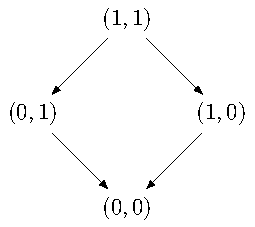
\includegraphics[scale = 0.8]{fig0}
%                 \caption{Одностоковая ориентация двумерного куба $G(\EE_2^2)$}\label{fig:hxy}
%             }
%         \end{figure}
%         Если $h(0, 1) = (0, 1)$ или $h(0, 1) = (1,1)$, то в соответствии с предыдущими рассуждениями мы можем аналогичным образом рассмотреть проекцию $x_i \gets 0$, получим функцию $f(x) = h(0, x)[2]$, для которой $f(0) = 0$, $f(1) = 1$, следовательно $f(x) = x$, и мы нашли самодвойственную проекцию.







%         Рассмотрим <<соседние>> по отношению к набору $\gamma = (0, \ldots, 0)$ наборы вида $e_i = (\underbrace{0, \ldots, 0}_{i-1}, 1, \underbrace{0, \ldots, 0}_{n-i})$.
%         Если существует такой набор $e_i$, что $g_i(e_i) \ne g_i(0, \ldots, 0)$, то достаточно рассмотреть проекцию $\gf$ вида 
%         \[
%             h(x) = \proj_{1, \ldots, i-1, i+1, \ldots, n}^{0, \ldots, 0}(\gf) \colon \EE_2^1 \to \EE_2^1.
%         \]
%         Тогда $h(1) \ne h(0)$, а значит, $h(1) = \overline{h(0)}$.
%         Таким образом, $h$~--- искомая самодвойственная проекция.

%         Осталось рассмотреть случай, в котором для всех наборов $\widetilde{\gamma^i}$ выполнено условие $g_i(\widetilde{\gamma^i}) = g_i(\gamma)$.
%         При этом если есть хотя бы один набор $\widetilde{\gamma^i}$, что $\gf(\widetilde{\gamma^i}) = \gf(\gamma)$, то мы можем перейти к размерности $n-1$, рассмотрев проекцию $\proj_{i}^{\overline{\gamma_i}}(\gf)$, для которой также выполняется условие утверждения.

%         Следовательно, остается случай, при котором для каждого $\widetilde{\gamma^i}$ найдется хотя бы одна позиция $j$, для которой $g_j(\widetilde{\gamma^i}) \ne g_j(\gamma)$.
%         Но в таком случае из неравенства следует, что $g_j(\widetilde{\gamma^i}) = \overline{g_j(\gamma)}$.
%         Тогда возьмем любое $i$ и рассмотрим проекцию на те координаты $j$, для которых $g_j(\widetilde{\gamma^i}) = g_j(\overline{\gamma})$. 
%         Индексов $j$ с таким условием будет не менее одного и не более $n-1$ по рассуждениям, приведенным ранее.
%         Полученная проекция также будет удовлетворять условиям леммы и иметь меньший размер.
%     \end{proof}

%     \begin{theorem}
%     \label{thm:self_proper}
%         Семейство $\ff_n$ булевых функций правильно тогда и только тогда, когда каждая из его проекций $\proj^{a_1, \ldots, a_k}_{i_1, \ldots, i_k}(\ff)$ не является самодвойственной булевой функцией.
%     \end{theorem}

%     \begin{proof}
%         Пусть $\ff_n$~--- правильное, $\gf = \proj^{a_1, \ldots, a_k}_{i_1, \ldots, i_k}(\ff)$~--- его проекция.
%         Предположим, что $\gf$~--- самодвойственное.
%         В таком случае, для любого $\alpha$ имеем $\gf(\alpha) = \overline{\gf(\overline{\alpha})}$.
%         Тогда для $\gf$ нарушается свойство правильности, следовательно, $\ff$ не является правильным (поскольку любая проекция правильного семейства должна быть правильной, см. утверждение~\ref{thm:proj}).

%         Докажем утверждение в обратную сторону. 
%         Для этого предположим, что $\ff_n$ не является правильным, и покажем, что в таком случае существует самодвойственная проекция.
%         Так как $\ff_n$ не является правильным, то найдутся два набора $\alpha = (\alpha_1, \ldots, \alpha_n)$ и $\beta = (\beta_1, \ldots, \beta_n)$, такие что для всех индексов $i$, в которых $\alpha$ и $\beta$ различны, $\alpha_i \ne \beta_i$, выполнено условие $\ff_i(\alpha) \ne \ff_i(\beta)$.
%         Рассмотрим проекцию $\gf$ семейства $\ff$ по тем координатам $j$, для которых $\alpha_j = \beta_j$. 
%         Для семейства $\gf$ выполнено следующее условие: существует набор $\gamma$ такой, что $\gf(\gamma) = \overline{\gf(\overline{\gamma})}$.
%         Тогда $\gf$ удовлетворяет условиям леммы~\ref{lemma:dual}, а значит, у этого семейства существует самодвойственная проекция, что и требовалось доказать.
%     \end{proof}


%%%%%%%%%%%%%%%%%%%%%%%%%%%%%%%%%%%%%%%%%%%%%%%%%%%%%%%%%

\section{Кликовое представление правильных семейств}
\label{sec:clique}

    В работах~\cite{sikiric2007cube, mathew2013enumerating} изучались \textquote{кубические замощения} пространства (англ.: cube tilings), а также подсчитывалось количество подобных неэквивалентных замощений (число классов изоморфизма) для разных размерностей замощаемого пространства (см. таблицу~\ref{tab:counttilings}).
    \begin{table}[h]
        \centering
        \captionsetup{justification=centering} % выравнивание подписи по-центру
        \caption{\label{tab:counttilings} Число неэквивалентных замощений пространства размерности $n$.}
        \begin{tabular}{|c|c|}
            \toprule
            Размер $n$  & Число замощений \\
            \midrule
            $n = 1$ & 2 \\
            \midrule
            $n = 2$ & 12 \\
            \midrule
            $n = 3$ & 744 \\
            \midrule
            $n = 4$ & 5541744 \\
            \midrule
            $n = 5$ & 638560878292512 \\
            \bottomrule
        \end{tabular}
    \end{table}
    
    Для $n = 1,2,3,4$ количество замощений пространства размерности $n$ совпадает с числом правильных булевых семейств размера $n$.
    Это совпадение неслучайно: в работе~\cite{borzechowski2022universal} было показано, что одностоковые ориентации булевых кубов находятся в биективном соответствии с замощениями пространства гиперкубами, а именно, было показано, что каждой одностоковой ориентации можно однозначно сопоставить клику в некотором графе специального вида (т.н. графы Келлера, см.~\cite{corradi1990combinatorial}).
    Обобщим этот результат на случай $k$-значный случай: покажем, что правильные семейства функций $k$-значной логики находятся в биективном соответствии с кликами графов, построенных аналогично графам Келлера (и совпадающих с этими графами при $k = 2$).

    \begin{definition}
        Пусть $G = (V, E)$~--- некоторый граф.
        Клика на $m$ вершинах в графе $G$~--- это подмножество вершин $V' \subseteq V$ размера $m$, такое что каждые две вершины $v, w \in V'$ соединены ребром в $G$: $\{v, w\} \in E$.
    \end{definition}

    Рассмотрим следующее обобщение графов Келлера на $k$-значный случай.

    \begin{definition}
        Зададим обобщенный граф Келлера $G(k, n)$ следующим образом:
        \begin{itemize}
            \item множество вершин графа $V$~--- наборы чисел от $0$ до $k^2-1$ длины $n$: 
            \[
                V = \EE_{k^2}^n;
            \]
            \item пара $\{v, w\}$ принадлежит множеству ребер $E$ тогда и только тогда, когда найдется координата $i$, $1 \le i \le n$, что выполнены два условия: 
            \[
                v_i \equiv w_i \text{ mod } \; k, \; v_i \ne w_i.
            \]
        \end{itemize}
    \end{definition}

    Будем рассматривать правильные семейства $\ff_n$ размера $n$ на $\EE_k^n$.
    Покажем, что они находятся во взаимно-однозначном соответствии с \textbf{кликами} в графе $G(k,n)$ размера $k^n$ (по правильному семейству строится клика в графе $G(k, n)$, и наоборот, по каждой клике размера $k^n$ в $G(k, n)$ задается правильное семейство на $\EE_k^n$).

    \begin{theorem}
        Каждой клике на $k^n$ вершинах в графе $G(k, n)$ можно поставить в биективное соответствие некоторое правильное семейство $\ff_n$ размера $n$ на $\EE_k^n$.
    \end{theorem}

    \begin{proof}
        Доказательство будет состоять из двух частей.
        Сначала рассмотрим вложение множества правильных семейств в множество клик графа $G(k, n)$, а затем покажем обратное: по каждой клике графа $G(k, n)$ построим некоторое правильное семейство $\ff_n$ размера $n$ на $\EE_k^n$.

        Рассмотрим некоторое правильное семейство $\ff = (f_1, \ldots, f_n)$ на $\EE_k^n$.
        Каждому набору $\xx = (x_1, \ldots, x_n) \in \EE_k^n$ поставим в соответствие набор из $\EE_{k^2}^n$ следующим образом.
        Для $a, b \in \EE_k$ определим число $\phi(a, b) =  k \cdot a + b \in \EE_{k^2}$, тогда набору $\xx$ поставим в соответствие набор 
        \[
            \xx \to \Phi_{\ff}(\xx) = \left( \phi(x_1, f_1(\xx)), \ldots, \phi(x_n, f_n(\xx)) \right) \in \EE_{k^2}^n.
        \]
        Повторим указанный процесс для каждого $\xx \in \EE_k^n$ и получим набор вершин в графе $G(k, n)$, построенный по семейству $\ff$.

        Полученное отображение $\Phi_{\ff}$ в множество вершин $V$ инъективно для каждого фиксированного правильного семейства $\ff$: если $\xx \ne \yy$, то $\Phi_{\ff}(\xx) \ne \Phi_{\ff}(\yy)$.
        Это следует из свойства правильности: найдется индекс $1 \le i \le n$, что $x_i \ne y_i$, но $f_i(\xx) = f_i(\yy)$, а значит, $\phi(x_i, f_i(\xx)) = k \cdot x_i + f_i(\xx) \ne k \cdot y_i + f_i(\yy) = \phi(y_i, f_i(\yy))$.
        Заметим также, что для полученных элементов выполняется условие 
        \[
            \phi(x_i, f_i(\xx)) \ne \phi(y_i, f_i(\yy)), \quad \phi(x_i, f_i(\xx)) \equiv \phi(y_i, f_i(\yy)) \; \mod k,
        \]
        а значит, полученные вершины графа соединены ребром в $G(k, n)$.
        Таким образом, отображение $\Phi_{\ff}$ задает по правильному семейству $\ff$ некоторый подграф графа $G(k ,n)$ на $k^n$ вершинах, причем любые две вершины в подграфе соединены ребром, а значит, составляют клику.

        Отображение $\ff \to \Phi_{\ff}$ также является инъективным (определяет различные клики при разных правильных семействах): если $\ff \ne \gf$, то существует $\xx \in \EE_k^n$, такой что $\ff(\xx) \ne \gf(\xx)$, но тогда $\Phi_{\ff}(\xx) \ne \Phi_{\gf}(\xx)$, и ни для какой точки $\yy \in \EE_k^n$ не может выполняться равенство $\Phi_{\ff}(\xx) = \Phi_{\gf}(\yy)$, а значит, точки $\Phi_{\ff}(\xx)$ нет в клике, задаваемой отображением $\Phi_{\gf}$.

        Рассмотрим теперь обратное отображение: каждому элементу $a \in \EE_{k^2}$ поставим в соответствие пару $(x, y) \in \EE_k^2$ вида 
        \[
            a \to \psi(a) = (a \text{ div } k, \; a \mod \; k),
        \]
        а каждому элементу $\vv = (v_1, \ldots, v_n) \in \EE_{k^2}^n$~--- пару векторов 
        \begin{gather*}
            (\xx, \yy) = \Psi(\vv) \in \left( \EE_{k}^n \right)^2, \\
            (x_i, y_i) = \psi(v_i), \; 1 \le i \le n.
        \end{gather*}
        Покажем, что при этом отображении клики перейдут в правильные семейства.

        Во-первых, такое отображение на кликах инъективно: если $\vv \ne \ww$, $\Psi(\vv) = (\xx, \alpha)$, $\Psi(\ww) = (\yy, \beta)$, $\vv$ и $\ww$ соединены ребром в графе $G(k, n)$, то найдется индекс $i$, для которого $v_i \ne w_i$, но $v_i \equiv w_i \mod k$, а значит, $x_i \ne y_i$.
        В силу того, что в каждой рассматриваемой клике $k^n$ вершин, указанное отображение ставит ей в соответствие множество пар $\{ (\xx, \alpha) \in \left( \EE_{k}^n \right)^2 \mid \xx \in \EE_k^n \}$, где первые элементы пар $\xx$ пробегают все множество $\EE_k^n$.

        Во-вторых, если мы интерпретируем второй элемент пары $\alpha$ как значение некоторого отображения $\ff \in P_k^n$ на элементе первой пары $\xx$ (т.е. $(\xx, \alpha) = (\xx, \ff(\xx))$), то семейство $\ff$ будет правильным, покажем это.
        Рассмотрим два неравных набора $\xx \ne \yy \in \EE_k^n$, а также их прообразы при отображении $\Psi$: $ \vv = \Psi^{-1}(\xx, \alpha)$, $ \ww = \Psi^{-1}(\yy, \beta)$.
        Для векторов $\vv$ и $\ww$ найдется индекс $1 \le i \le n$, для которого $v_i \ne w_i$, но $v_i \equiv w_i \mod k$ (поскольку $\vv$ и $\ww$ соединены ребром в $G(k, n)$), а значит, $x_i \ne y_i$, но при этом $\alpha_i = \beta_i$, т.е. выполнено условие правильности.
    \end{proof}

    %\TODO{подумать, как связаны изоморфизмы графа $G(k, n)$ и изометрии правильных семейств.}

    %\TODO{что хорошего ещё можно сказать про это всё?}


\section{Неортогональность аффинных подпространств}
\label{sec:nonortho}

    Рассмотрим одно обобщение результата~\cite[теорема~6]{ruet2015asynchronous}, касающегося ортогональности подпространств булева куба.
    Указанный результат также был сформулирован для $\hupf$-сетей.
    На язык правильных семейств он <<переводится>> в более общей формулировке, но за счет некоторого ослабления понятия правильности в случае $k$-значных логик при $k \ge 3$ (см. определение~\ref{def:genericproper}).

    \begin{definition}
        Пусть $\xx, \yy \in Q^n$~--- два набора из $n$ элементов, обозначим через $[\xx, \yy]$ множество таких элементов $\vv \in Q^n$, что $\vv$ совпадает с $\xx$ в тех номерах координат, где $x_i = y_i$:
        \[
            [\xx, \yy] = \{\vv \in Q^n \mid v_i = x_i = y_i \text{ для всех $i$, где } x_i = y_i\}.
        \]
        Будем называть $[\xx, \yy]$ подпространством в $Q^n$.
    \end{definition}

    \begin{remark}
        В случае $Q = \ZZ_k$ нетрудно видеть, что $[\xx, \yy]$~--- это аффинное подпространство в $\ZZ_k^n$.
    \end{remark}
    
    \begin{definition}
        Пусть $[\xx, \yy]$ и $[\ww, \vv]$~--- два подпространства.
        Обозначим через $I = \{ i_1, \ldots, i_s \}$ все позиции, для которых $x_{i_j} \ne y_{i_j}$; обозначим через $L = \{ \ell_1, \ldots, \ell_t \}$ все позиции, для которых $w_{\ell_j} \ne v_{\ell_j}$.
        Будем говорить, что $[\xx, \yy]$ и $[\ww, \vv]$ ортогональны (и писать $[\xx, \yy] \perp [\ww, \vv]$), если выполнено следующее условие: $I \cap J = \varnothing$.
    \end{definition}

    \begin{example}[Ортогональность в случае $Q = \ZZ_k$]
        Рассмотрим случай $Q = \ZZ_k$.
        Тогда $[\xx, \yy]$ и $[\ww, \vv]$ являются аффинными подпространствами $\ZZ_k^n$.
        Пусть $[\xx, \yy] = \alpha + \mathcal{L}_1$, $[\ww, \vv] = \beta + \mathcal{L}_2$, тогда $[\xx, \yy] \perp [\ww, \vv]$ тогда и только тогда, когда $\mathcal{L}_1$ и $\mathcal{L}_2$ перпендикулярны (как векторные подпространства) относительно билинейной формы $\langle \xx \mid \yy \rangle = \sum_{i=1}^n x_i \cdot y_i$, то есть для любых $\xx \in \mathcal{L}_1$ и $\yy \in \mathcal{L}_2$ выполняется $\langle \xx \mid \yy \rangle = 0$.
    \end{example}

    Теперь сформулируем необходимое условие правильности семейства в терминах ортогональных подпространств.

    \begin{theorem}
        \label{propos:nonortho}
        Если семейство $\ff_n \colon Q^n \to Q^n$ правильно, то для любых неравных $\xx, \yy \in Q^n$ выполнено условие не-ортогональности:
        \[
            [\xx, \yy] \not \perp [\xx \circ \ff_n(\xx), \yy \circ \ff_n(\yy)].
        \]
    \end{theorem}

    \begin{proof}
        Пусть $\ff$~--- правильное.
        Тогда по определению найдется такой индекс $i$, что $x_i \ne y_i$, но $f_i(x) = f_i(y)$.
        Но отсюда следует, что $x_i \circ f_i(x) \ne y_i \circ f_i(y)$.
        Следовательно, нашлась общая для $[\xx, \yy]$ и $[\xx \circ \ff(\xx), \yy \circ \ff(\yy)]$ координата $i$ такая, что $x_i \ne y_i$ и $x_i \circ f_i(x) \ne y_i \circ f_i(y)$.
        Это по определению влечет не-ортогональность соответствующих пространств.
    \end{proof}

    Обратное утверждение не всегда верно.
    \begin{example}
        Рассмотрим случай $k = 3$, $n=1$, $\ff(x) = x$, $\circ = +$.
        В таком случае:
        \begin{itemize}
            \item семейство $\ff$ не является правильным, так как зависит существенно от $x$;
            \item для семейства $\ff$ выполнено условие не-ортогональности: для любых неравных $x \ne y$ имеем
            \begin{gather*}
                [x, y] = \EE_3, \; x + f(x) = 2x \ne y + f(y) = 2y, \\
                [x + f(x), y + f(y)] = \EE_3.
            \end{gather*}
        \end{itemize}
    \end{example}

    Однако мы можем ввести понятие \textquote{обобщенного правильного семейства}, для которого условие \textquote{обобщенной правильности} будет эквивалентно условию отсутствия ортогональных аффинных подпространств указанного выше вида.

    \begin{definition}
    \label{def:genericproper}
        Пусть $(Q, \circ)$~--- квазигруппа.
        Будем называть семейство $\ff_n \colon Q^n \to Q^n$ обобщенно правильным, если для любых двух неравных наборов $\xx, \yy \in Q^n$ найдется индекс $i$, такой что выполнены условия:
        \[
            x_i \ne y_i, \quad x_i \circ f_i(\xx) \ne y_i \circ f_i(\yy).
        \]
    \end{definition}

    \begin{remark}
        Отметим два факта:
        \begin{itemize}
            \item правильные семейства являются обобщенно правильными: для правильных семейств найдется индекс $i$, что $x_i \ne y_i$, но $f_i(\xx) = f_i(\yy)$, откуда следует $x_i \circ f_i(x) \ne y_i \circ f_i(y)$;
            \item для булева случая понятия правильности и обобщенной правильности эквивалентны: фактически, сформулированное выше характеристическое свойства эквивалентно свойству отсутствия т.н. \textquote{зеркальных пар} у семейства булевых функций (см.~\cite[раздел~3]{ruet2016local}).
        \end{itemize}
    \end{remark}

    \begin{theorem}
        Семейство $\ff_n \colon Q^n \to Q^n$ является обобщенно правильным тогда и только тогда, когда выполнено условие не-ортогональности аффинных подпространств: для любых двух неравных наборов $\xx, \yy \in Q^n$ выполняется
        \[
            [\xx, \yy] \not \perp [\xx \circ \ff(\xx), \yy \circ \ff(\yy)]
        \]
    \end{theorem}

    \begin{proof}
        В прямую сторону утверждение доказывается аналогично утверждению~\ref{propos:nonortho}.
        В обратную сторону утверждение также является простым следствием определения ортогональности.
    \end{proof}

    \begin{theorem}
        \label{propos:bijection}
        Пусть семейство $\ff \colon Q^n \to Q^n$ обобщенно правильное.
        Тогда отображение $\sigma_{\ff} \colon Q^n \to Q^n$, переводящее $\xx \in Q^n$ в $\xx \circ \ff(\xx)$, является биективным.
    \end{theorem}

    \begin{proof}
        Докажем инъективность отображения $\sigma_{\ff}$: по определению обобщенной правильности для любых $\xx \ne \yy$ найдется индекс $i$ такой, что 
        \[
            x_i \circ f_i(\xx) = \sigma_{\ff}(\xx)[i] \ne \sigma_{\ff}(\yy)[i] = y_i \circ f_i(\yy).
        \]
        Биективность следует из конечности $Q^n$.
    \end{proof}

\section*{Выводы}

    В этой главе мы рассмотрели несколько альтернативных способов описания булева правильного семейства:
    \begin{itemize}
        \item характеризация в терминах одностоковой ориентации (т.н.~$\mathsf{USO}$-ориентации булева куба);
        \item характеризация в терминах булевой сети с наследственно неподвижной точкой (т.н.~$\hupf$-сети);
        %\item характеризация в терминах булева отображения, каждая проекция которого не является самодвойственной,
        \item характеризация в терминах клик обобщенных графов Келлера.
    \end{itemize}
    Также было введено понятие обобщенно правильного семейства и его альтернативная характеризация в терминах ортогональности подпространств (в случае $k=2$ понятие обобщенно правильного семейства совпадает с понятием правильного семейства).

    Таким образом, один и тот же объект (правильные семейства) может быть рассмотрен сразу с нескольких точек зрения, а результаты, полученные в рамках одного \textquote{языка}, могут быть перенесены на другой \textquote{язык} (часто даже в более общем виде).
    При этом геометрическая интуиция позволяет ввести некоторые новые классы семейств, такие как рекурсивно и локально треугольные семейства, а также доказать некоторые свойства правильных семейств (например, $\mathsf{coNP}$-полноту задачи распознавания правильности по схеме из функциональных элементов~\cite{USOcomplexity, galatenko21generation} или оценку на число булевых правильных семейств).
           % Глава 2
\chapter{Свойства правильных семейств}\label{sec:properties}

\section{Группа преобразований, сохраняющих правильность}
    В разделе~\ref{sec:proper_properties} было показано, что сдвиги (внутренние и внешние), а также согласованные перестановки семейства сохраняют свойство семейства <<быть правильным>>.
    В настоящем разделе мы рассмотрим обратную задачу.
    Пусть $\Phi$, $\Psi$~--- биекции на множестве $Q^n$: $\Phi, \Psi \in \SSS_{Q^n}$.
    При каких условиях на $\Phi$, $\Psi$ отображение $x \to \Phi(\ff(\Psi(x)))$ также будет являться правильным для правильных семейств $\ff$?
    Другими словами, каков стабилизатор для множества правильных семейств $\ff_n$ размера $n$ при действии $(\Phi, \Psi) \curvearrowright \ff \colon x \to \Phi(\ff(\Psi(x)))$?
    Далее мы покажем, что такими $\Phi$ и $\Psi$ могут быть только согласованные перестановки семейства (см. определение~\ref{def:sigma}) совместно с перекодировками (см. определение~\ref{def:reencoding}). 

\subsection{Перекодировки и изометрии пространства $Q^n$}
\label{sec:reencoding}

    Дадим несколько предварительных определений.
    \begin{definition}[перекодировка вектора]
    \label{def:vec_reencoding}
        Перекодировкой вектора $\xx \in Q^n$ будем называть вектор $\yy$ вида $\yy =  (\phi_1(x_1), \ldots, \phi_n(x_n))$, где $\phi_i \in \SSS_Q$.
    \end{definition}

    \begin{definition}[перекодировка семейства]
    \label{def:reencoding}
        Перекодировкой семейства $\ff_n$, заданного на $Q^n$, будем называть семейство $\gf$ вида:
        \[
            \gf(\xx) = 
            \begin{bmatrix}
                \phi_1(f_1(\psi_1(x_1), \ldots, \psi_n(x_n))) \\
                \vdots \\
                \phi_n(f_n(\psi_1(x_1), \ldots, \psi_n(x_n)))
            \end{bmatrix},
        \]
        где $\phi_i, \psi_i \in \SSS_Q$.
    \end{definition}

    \begin{remark}
        Перекодировка семейства является композицией перекодировки аргумента функции (как вектора) и перекодировки полученного вектора значения функции.
    \end{remark}

    Как было отмечено ранее (см. теорему~\ref{thm:sigma}), согласованные перестановки сохраняют свойство правильности.
    Аналогичное свойство выполняется и для перекодировок (см.~\cite[Лемма~2]{galatenko21criterion}).

    \begin{proposition}[перекодировки семейства сохраняют правильность]
        Если $\ff_n$~--- правильное семейство, то любая перекодировка $\gf_n$ семейства $\ff_n$ также является правильным семейством.
    \end{proposition}

    Там же (см.~\cite[Теорема~1]{galatenko21criterion}) доказан следующий критерий правильности семейства в терминах перекодировок.

    \begin{proposition}[эквивалентное определение правильности, $k$-значный случай]
    \label{thm:reencoding_properness}
        Семейство $\ff_n$ на $Q^n$ является правильным тогда и только тогда, когда любая перекодировка любой проекции $\ff_n$ (в том числе и тривиальная проекция) имеет единственную неподвижную точку.
    \end{proposition}

    Заметим, что перекодировки и перестановки вектора (см. определение~\ref{def:sigma_vec}) сохраняют (не)равенство координат вектора.
    Другими словами, если $d(\xx, \yy)$~--- метрика Хэмминга на пространстве $Q^n$, то для перекодировок и перестановок вектора $\Phi$ выполняется равенство 
    \[
        d(\xx, \yy) = d(\Phi(\xx), \Phi(\yy)).
    \]
    Это наблюдение побуждает поставить следующий вопрос: верно ли, что преобразования, сохраняющие правильность, обязаны быть изометриями пространства $Q^n$? 
    Далее мы утвердительно ответим на этот вопрос.

    \begin{definition}[Изометрии пространства $Q^n$]
        Пусть $Q^n$ рассматривается как метрическое пространство с метрикой Хэмминга
        \[
            d(\xx, \yy) = \lvert \left\{ i \mid x_i \ne y_i \right\} \rvert,
        \]
        тогда группой изометрий $Iso(Q^n)$ пространства $Q^n$ будем называть множество отображений 
        \[
            Iso(Q^n) = \left\{ \Phi \in \SSS_{Q^n} \mid d(\Phi(\xx), \Phi(\yy)) = d(\xx, \yy) \; \forall \xx, \yy \in Q^n \right\}
        \]
        с операцией композиции отображений.
    \end{definition}

    Нам также понадобится понятие слабой изометрии как отображения, которое сохраняет расстояние между точками, находящимися на строго определенном фиксированном расстоянии.

    \begin{definition}[Слабые изометрии пространства $Q^n$]
        Будем называть $p$-изометрией (слабой изометрией) биективное отображение $\Phi \colon Q^n \to Q^n$ с тем свойством, что оно сохраняет расстояние между точками, которые находятся на расстоянии~$p$:
        \[
            \left\{ \Phi \in \SSS_{Q^n} \mid d(\Phi(\xx), \Phi(\yy)) = d(\xx, \yy) \; \forall \xx, \yy \in Q^n, \; d(\xx, \yy) = p \right\}.
        \]
    \end{definition}

    \begin{remark}
    \label{rem:isop_group}
        Легко увидеть, что $p$-изометрии образуют группу (в частности, обратное к $p$-изометрии преобразование также является \mbox{$p$-изометрией}).
    \end{remark}

    Приведем два результата, связывающих множество слабых изометрий и изометрий пространств с метрикой Хэмминга.

    \begin{proposition}[{\cite[Теорема~1]{krasin06}, \cite[Лемма~1]{de2016weak}}]
    \label{propos:bool_iso}
        Если $\Phi$ является 1-изометрией $Q^n$, $\lvert Q \rvert = 2$, то $\Phi$ является изометрией $Q^n$.
    \end{proposition}

    \begin{proposition}[{\cite[Теорема~4.1]{de2016weak}}]
    \label{propos:k_iso}
        Если $\Phi$ является 1-изометрией $Q^n$, $\lvert Q \rvert > 2$, $n > 2$, то $\Phi$ является изометрией $Q^n$.
    \end{proposition}

    \begin{remark}
        Из формулировки лемм~\ref{propos:bool_iso} и~\ref{propos:k_iso} видно, что существуют особые случаи, не покрываемые приведенными выше утверждениями.
        Рассмотрим каждый из них более подробно.
        
        Случай $k > 2$, $n = 1$ тривиален: любая биекция в указанном вырожденном случае является изометрией.
        
        Случай $k > 2$, $n = 2$: пусть $\Phi$ является 1-изометрией и биекцией.
        Покажем, что $\Phi$ также сохраняет расстояние 2.
        Пусть $\alpha, \beta \in Q^2$, $d(\alpha, \beta) = 2$.
        В силу биективности $d(\Phi(\alpha), \Phi(\beta)) > 0$.
        Предположим, что $d(\Phi(\alpha), \Phi(\beta)) = 1$.
        В таком случае, поскольку $\Phi^{-1}$ также является 1-изометрией (см. замечание~\ref{rem:isop_group}), мы имеем противоречие:
        \[
            1 = d\left(\Phi(\alpha), \Phi(\beta) \right) = d \left(\Phi^{-1}(\Phi(\alpha)), \Phi^{-1}(\Phi(\beta)) \right) = d \left( \alpha, \beta \right) = 2.
        \]
        Других значений расстояния в случае $n = 2$ не бывает.
    \end{remark}

    Таким образом, мы доказали следующее вспомогательное утверждение.
    \begin{lemma}
    \label{lemma:main_iso}
        Группа 1-изометрий для пространства $Q^n$ с метрикой Хэмминга совпадает с группой всех изометрий.
    \end{lemma}
    Также для пространств Хэмминга верно следующее утверждение, устанавливающее связь между изометриями $Q^n$ и ранее введенными преобразованиями векторов.

    \begin{proposition}[{\cite{chirivi}}]
    \label{propos:iso}
        Группа изометрий $Iso(Q^n)$ состоит из перестановок (см. определение~\ref{def:sigma_vec}) и перекодировок (см. определение~\ref{def:vec_reencoding}) векторов.
    \end{proposition}

\subsection{Группа биективных преобразований, сохраняющих правильность}

    Нашей задачей является доказательство того факта, что если $\Phi$ и $\Psi$~--- биекции, и $\Phi(\ff(\psi(x)))$~--- правильное семейство для любого правильного семейства $\ff_n$, то $\Phi$, $\Psi$ являются изометриями пространства $Iso(Q^n)$: $\Phi, \Psi \in Iso(Q^n)$.
    Для этого мы сначала докажем, что $\Phi$ и $\Psi$ обязаны являться $1$-изометриями (утверждения~\ref{propos:inner_iso} и~~\ref{propos:outer_iso}).
    Затем мы воспользуемся утверждениями~\ref{propos:bool_iso} и~\ref{propos:k_iso}, чтобы показать, что $\Phi$ и $\Psi$ являются изометриями $Q^n$.
    Наконец, мы применим утверждение~\ref{propos:iso} совместно с некоторыми дополнительными соображениями и покажем, что биективные преобразования, сохраняющие правильность семейств, исчерпываются перекодировками и согласованными перестановками семейства (теорема~\ref{thm:propergroup}).

    \begin{remark}
        Мы рассматриваем только пары биективных преобразований.
        Так, например, в указанные преобразования не входят преобразования вида $f_n(x_1, \ldots, x_n) \to a$, $a \in E_k$, $f_i(x_1, \ldots, x_n) \to f_i(x_1, \ldots, x_{n-1}, a)$, $1 \le i \le n-1$ (комбинация проекции семейства с дополнением константой), которые тоже сохраняют правильность.
    \end{remark}

    \begin{proposition}
        \label{propos:notmirror}
        Пусть $\alpha$, $\beta \in Q^n$~--- два не-противоположных набора (т.е. $d(\alpha, \beta) < n$).
        Тогда существует правильное семейство $\ff_n$ и точки $\xx$, $\yy$, такие что $\ff(\xx) = \alpha$, $\ff(\yy) = \beta$.
    \end{proposition}

    \begin{proof}
        Достаточно рассмотреть правильным образом подобранное треугольное семейство.
        Без ограничения общности будем предполагать, что первые $k$ координат наборов совпадают:
        \[
            \alpha_1 = \beta_1, \ldots, \alpha_k = \beta_k, k \ge 1.
        \]
        В таком случае зададим первые $k$ функций треугольного семейства как константы $f_i \equiv \alpha_i$; оставшиеся $(n-k)$ функций зададим так, чтобы на некотором фиксированном $\xx_0$ они принимали значение $\alpha_{k+1}, \ldots, \alpha_n$, на некотором фиксированном $\yy_0$ (отличном от $\xx_0$ в первых $k$ координатах)~--- значение $\beta_{k+1}, \ldots, \beta_n$.
        Мы получим семейство вида 
        \[
            \begin{bmatrix}
                \alpha_1 \\
                \vdots \\
                \alpha_k \\
                \ff_{n-k}(x_1, \ldots, x_k)
            \end{bmatrix},
        \]
        которое является треугольным и обладает требуемым свойством.
    \end{proof}

    \begin{proposition}
    \label{propos:inner_iso}
        Пусть $\gf(\xx) = \Phi(\ff(\Psi(x)))$~--- правильное для всех $\ff_n$, заданных на $Q^n$, $\Phi$ и $\Psi$~--- биекции $Q^n \to Q^n$.
        Тогда $\Psi$ является 1-изометрией пространства Хэмминга $Q^n$.
    \end{proposition}

    \begin{proof}
        Докажем отрицание: если $\Psi$ не является 1-изометрией, $\Phi$ и $\Psi$ биективны, то существует такое правильное семейство $\ff_n$ на $Q^n$, что $\gf(\xx) = \Phi(\ff(\Psi(\xx)))$~--- не является правильным.

        Так как $\Psi$~--- не 1-изометрия, то найдутся наборы $\xx_1$, $\xx_2$, что $d(\xx_1, \xx_2) = 1$, но $d(\Psi(\xx_1), \Psi(\xx_2)) > 1$ (заметим, что указанное расстояние не может быть равно 0, т.к. $\Psi$ биективно).
        Пусть для определенности $\xx_1$ и $\xx_2$ различны только в $i$-й координате, и найдутся такие индексы $j_1, j_2$, что $\Psi(\xx_1)$ и $\Psi(\xx_2)$ различны в позициях $j_1$ и $j_2$.
        Подберем такое семейство $\ff_n$, что выполнено неравенство
        \[
            \gf_i(\xx_1) = \Phi(\ff(\Psi(\xx_1)))[i] \ne \Phi(\ff(\Psi(\xx_2)))[i] = \gf_i(\xx_2).
        \]

        Рассмотрим множество пар точек $(\ww_1, \ww_2)$, $\ww_1, \ww_2 \in Q^n$, таких что $\ww_1[i] \ne \ww_2[i]$.
        Число таких пар точек равно $k^{2n-1}(k-1)$ (есть $k^n$ способов зафиксировать $\ww_1$ и $k^{n-1}(k-1)$ способов зафиксировать $\ww_2$).
        Теперь рассмотрим множество пар точек $(\yy_1, \yy_2) = (\Phi^{-1}(\ww_1), \Phi^{-1}(\ww_2))$.
        Среди таких пар найдется пара со свойством $\yy_1[j_1] = \yy_2[j_1]$ или $\yy_1[j_2] = \yy_2[j_2]$, поскольку число пар, не удовлетворяющих этому свойству, равно $k^{2n-2}(k-1)^2$, что меньше числа $k^{2n-1}(k-1)$.

        Таким образом, найдутся две точки $\yy_1$, $\yy_2$ со свойствами:
        \begin{itemize}
            \item $\Phi(\yy_1)[i] \ne \Phi(\yy_2)[i]$;
            \item $\yy_1[j] = \yy_2[j]$, где $j \in \{j_1, j_2\}$.
        \end{itemize}
        Построим по этим точкам семейство $\ff$ так, чтобы $\ff(\Psi(\xx_1)) = \yy_1$, $\ff(\Psi(\xx_2)) = \yy_2$.

        Для этого рассмотрим треугольное семейство $\ff$, такое что $f_j(\cdot) \equiv \yy_1[j]$, а остальные функции зависят от $j$-той переменной таким образом, что если она принимает значение $\Psi(\xx_1)[j]$, то все семейство равно $\yy_1$, а если она принимает значение $\Psi(\xx_2)[j]$, то все семейство равно $\yy_2$.

        В таком случае мы будем иметь:
        \begin{itemize}
            \item $\ff$~--- правильное семейство (в силу треугольности),
            \item $\Phi(\ff(\Psi(\xx_1)))[i] = \Phi(\yy_1)[i] \ne \Phi(\ff(\Psi(\xx_2)))[i] = \Phi(\yy_2)[i]$,
        \end{itemize}
        а значит, семейство $\gf(x)$ не является правильным (нарушено условие правильности на паре наборов $\xx_1$, $\xx_2$).
    \end{proof}

    \begin{remark}
        Из доказанного утверждения и утверждений~\ref{propos:bool_iso} и~\ref{propos:k_iso} следует, что $\Psi$ является изометрией метрики Хэмминга.% (кроме, быть может, особых случаев $k = 2$, $n = 3$ и $k > 2$, $n = 2$).
    \end{remark}

    \begin{proposition}
    \label{propos:outer_iso}
        Пусть $\gf(\xx) = \Phi(\ff(\Psi(x)))$~--- правильное для всех $\ff_n$, заданных на $Q^n$, $\Phi$ и $\Psi$~--- биекции $Q^n \to Q^n$.
        Тогда $\Phi$ является 1-изометрией пространства Хэмминга $Q^n$.
    \end{proposition}

    \begin{proof}
        Случай биективного отображения $\Psi$, не являющегося изометрией, был разобран ранее, поэтому мы можем предполагать, что $\Psi$~--- изометрия.

        Предположим, что $\Phi$~--- не 1-изометрия.
        Это означает, что найдутся наборы $\yy_1, \yy_2 \in Q^n$, такие что $d(\yy_1, \yy_2) = 1$, но $d(\Phi(\yy_1), \Phi(\yy_2)) = t > 1$ (указанное расстояние не может быть равно 0, т.к. $\Phi$~--- биекция).
        Для определенности обозначим за $j$ индекс, в котором $\yy_1$ и $\yy_2$ различаются: $\yy_1[j] \ne \yy_2[j]$.

        Если мы предположим, что $t = n$, то по предложению~\ref{propos:notmirror} мы можем найти правильное семейство $\ff_n$, которое принимает оба значения $\yy_1$ и $\yy_2$ на некоторых $\xx_1$, $\xx_2$.
        Но тогда $\Phi(\ff_n(\Psi(x)))$ не может быть правильным, так как принимает противоположные значения.

        Следовательно, мы имеем $1 < t < n$.
        Будем считать без ограничения общности, что $\Phi(\yy_1)$ и $\Phi(\yy_2)$ различаются в первых $t$ индексах: $\Phi(\yy_1)[i] \ne \Phi(\yy_2)[i]$, $1 \le i \le t$. 
        
        Построим два набора $\xx_1, \xx_2 \in Q^n$ и правильное семейство $\ff_n$ так, что выполняются условия:
        \[
            \ff_n(\Psi(\xx_1)) = \yy_1, \ff_n(\Psi(\xx_2)) = \yy_2,
        \]
        при этом потребуем, чтобы 
        \begin{itemize}
            \item $\xx_1[i] = \xx_2[i]$ при $t+1 \le i \le n$, 
            \item $\xx_1[i] \ne \xx_2[i]$ при $1 \le i \le t$.
        \end{itemize}
        Поскольку $\Psi$ по предположению является изометрией, то $d(\Psi(\xx_1), \Psi(\xx_2)) = t > 1$, следовательно, найдется $j' \ne j$, такой что $\Psi(\xx_1)[j'] \ne \Psi(\xx_2)[j']$.
        Зададим $j$-ю функцию семейства $\ff_n$ следующим образом:
        \begin{itemize}
            \item $\yy_1[j]$, если $j'$-я переменная принимает значения $\Psi(x_1)[j']$,
            \item $\yy_2[j]$, если $j'$-я переменная принимает значения $\Psi(x_2)[j']$.
        \end{itemize}
        Остальные функции $f_i$ положим равными тождественно $\yy_1[i]$, где $1 \le i \le n$, $i \ne j$.
        Полученное семейство является треугольным, а следовательно, правильным.
        Для семейства $\gf(\xx) = \Phi(\ff(\Psi(\xx)))$ условие правильности нарушается на наборах $\xx_1$ и $\xx_2$.
        Мы предположили, что $\Phi$ не является 1-изометрией, и пришли к противоречию, из которого следует утверждение.
    \end{proof}

    \begin{remark}
        Из доказанного утверждения и утверждений~\ref{propos:bool_iso} и~\ref{propos:k_iso} следует, что $A$ является изометрией метрики Хэмминга. %(кроме, быть может, особых случаев $k = 2$, $n = 3$ и $k > 2$, $n = 2$).
    \end{remark}

    \begin{theorem}
    \label{thm:propergroup}
        Пусть $\gf(\xx) = \Phi(\ff(\Psi(x)))$~--- правильное для всех $\ff_n$, заданных на $Q^n$, $\Phi$ и $\Psi$~--- биекции $Q^n \to Q^n$.
        Тогда $\Phi$ и $\Psi$ имеют вид $\Phi = \sigma \circ A$, $\Psi = \sigma \circ B$, где 
        \begin{itemize}
            \item $\sigma \in \SSS_n$ (перенумерация координат вектора),
            \item $A, B \in \left( \SSS_Q \right)^n$ (перекодировка вектора). 
        \end{itemize}
    \end{theorem}

    \begin{proof}
        Мы уже показали, что $\Phi$ и $\Psi$ обязаны быть изометриями $Q^n$.
        Из утверждения~\ref{propos:iso} следует, что $\Phi = (\sigma_1 \circ A)$, $\Psi = (\sigma_2 \circ B)$, где $\sigma_1, \sigma_2 \in \SSS_n$, $A, B \in \left( \SSS_Q \right)^n$.
        Покажем, что в таком случае $\sigma_1 = \sigma_2$ (т.е. перенумерация семейства должна быть согласована).

        Применение покомпонентных преобразований $A$ и $B$ не меняет свойства правильности, поэтому можно ограничиться случаем рассмотрения $\Phi = (\sigma_1 \circ I)$, $\Psi = (\sigma_2 \circ I)$, где $I$~--- тождественное преобразование $Q^n \to Q^n$.
        Пусть $\sigma_1 \ne \sigma_2$.
        Тогда существуют $i$ и $j$ со свойством $\sigma_1(i) = \sigma_2(j) = s$, при этом $i \ne j$.
        В таком случае достаточно рассмотреть треугольное семейство $f_i(x_j) = x_j$, $f_l \equiv const$, $l \ne i$.
        Под действием $(\Phi, \Psi) \curvearrowright \ff$ семейство $\ff$ перейдет в семейство, включающее в себя функцию $f_{\sigma_1(i)}(x_{\sigma_2(j)}) = f_s(x_s) = x_s$, что противоречит правильности.
    \end{proof}

    \begin{remark}
        Заметим, что в булевом случае $k=2$ перекодировки семейства исчерпываются сдвигами.
        Для одностоковых ориентаций булева куба (см. раздел~\ref{sec:uso}) внешние и внутренние сдвиги, равно как и согласованная перенумерация сохраняют свойство ориентации быть одностоковой (подробнее см.~\cite[Лемма~4.4]{USOphd}).
        Таким образом, в булевом случае имеется взаимно-однозначное соответствие между <<алгебраическим>> и <<геометрическим>> описанием семейства.
        В случае $k$-значной логики группа преобразований, сохраняющих правильность, является более широкой, чем группа преобразований, сохраняющих <<одностоковость>>, и указанное соответствие разрушается.
    \end{remark}



\subsection{Отношение эквивалентности на множестве правильных семейств}
    Действие группы $\GGG$ на множестве правильных семейств позволяет говорить об отношении эквивалентности между правильными семействами.
    \begin{definition}
        Два семейства $\ff_n$ и $\gf_n$ на $Q^n$ назовем эквивалентными, если существует преобразование $\Phi \in \GGG$, переводящее семейство $\ff_n$ в семейство $\gf_n$.
    \end{definition}
    Таким образом можно говорить о классах эквивалентности семейств, а также о системе представителей для всех семейств размера $n$.

    \TODO{Дописать алгоритм для порождения представителей.}







\section{Образы и пробразы при действии правильного семейства}

    В этом разделе мы будем рассматривать булево семейство $\ff_n$ как отображение $\ZZ_2^n \to \ZZ_2^n$:
    \begin{equation*}
        \xx = \begin{bmatrix}
            x_1 \\
            \vdots \\
            x_n
        \end{bmatrix}
        \to \ff_n(\xx) = 
        \begin{bmatrix}
            f_1(x_1, \ldots, x_n) \\
            \vdots \\
            f_n(x_1, \ldots, x_n)
        \end{bmatrix}.
    \end{equation*}

    Как было показано в работе~\cite{galatenko23}, мощность образа правильного семейства является важной характеристикой, которая, в частности, определяет, какое количество различных $d$-квазигрупп может быть порождено с помощью конструкции, описанной в теореме~\ref{thm:dquasi_proper}.

    Для правильных семейств выполняется следующее ограничение на мощность образа~\cite[Теорема~5]{galatenko23}.
    \begin{theorem}
        \label{thm:image}
        Число значений, принимаемых правильным семейством порядка~$n$ в $k$-значной логике, не превосходит~$k^{n-1}$.
    \end{theorem}


\subsection{Мощность прообраза при действии правильного семейства}
\label{sec:preimage_boolean}

    Зададимся следующим вопросом. 
    Пусть дана точка $\alpha \in \ZZ_2^n$.
    Что в таком случае можно сказать о мощности множества прообразов точки $\alpha$ при действии отображения $\ff_n$:
    \[
        \ff_n^{-1}(\alpha) = \{\xx \in \ZZ_2^n \mid \ff_n(\xx) = \alpha \}.
    \]
    Оказывается, что для правильных семейств булевых функций верно следующее утверждение~\cite{dm21}.

    \begin{theorem}[Четность мощности множества прообразов]
    \label{thm:preimage}
        Пусть $\ff_n$~--- правильное семейство булевых функций.
        Тогда для любого $\alpha \in \{0, 1\}^n$ число решений уравнения $\ff_n(\xx) = \alpha$ всегда четно.
    \end{theorem}

    \begin{remark}
    \label{rem:eqn}
        Случай уравнения $\ff_n(\xx) = \alpha$ можно свести к рассмотрению уравнения $\ff_n(\xx) =  0^n$.
        Используя теорему~\ref{thm:outer_shift}, можно утверждать, что если $\ff_n(\xx)$~--- правильное семейство, то и $\gf(\xx) = \ff(\xx) \oplus \alpha$ также является правильным.
        При этом $\xx^*$ является решением уравнения $\ff(x) = \alpha$ тогда и только тогда, когда $\xx^*$ является решением уравнения $\gf(\xx) = 0^n$.
    \end{remark}

    \begin{proof}
        Используя замечание~\ref{rem:eqn}, достаточно доказать, что уравнение $\ff_n(\xx) = 0^n$ всегда имеет четное число решений, где $\ff_n$~---~правильное семейство булевых функций размера $n$.
        Будем вести доказательство индукцией по размеру правильного семейства.

        \textbf{База индукции $(n=1)$:} семейства размера 1~---~это константные функции
        \begin{gather*}
            0(x_1) \equiv 0, \\
            1(x_1) \equiv 1.
        \end{gather*} 
        Очевидно, что для этих двух семейств уравнение $\ff_n(x_1) = 0$ имеет 2 или 0 решений соответственно.

        \textbf{Предположение индукции:} допустим, что уравнение $\gf_k(\xx) = 0^k$ имеет четное число решений для любого правильного семейства $G$ размера $k \le n$.
        Пусть теперь нам дано правильное булево семейство $\ff_{n+1}$ размера $n+1$.
        Введем обозначение $\xx = (x_1, \ldots, x_n)$.
        По свойству правильности мы можем утверждать, что $f_{n+1}$ не зависит существенно от переменной $x_{n+1}$ (см. замечание~\ref{rem:essential_general}).
        С учетом этого замечания мы можем считать, что $f_{n+1}$ зависит только от первых $n$ переменных, то есть от $\xx$.
        Тогда верно следующее разложение:
        \[
            \ff_{n+1}(x_1, \ldots, x_{n+1}) = 
            \begin{bmatrix}
                x_{n+1} \cdot \ff^1(\xx) \oplus \overline{x_n} \cdot \ff^0(\xx) \\
                f_{n+1}(\xx)
            \end{bmatrix},
        \]
        где за $\ff^b(x)$, $b \in \{0, 1\}$, обозначены семейства-проекции
        \[
            \ff^b(\xx) = \proj_{n+1}^b(\ff_{n+1}) = 
            \begin{bmatrix}
                f_1(x_1, \ldots, x_{n}, b) \\
                \vdots \\
                f_{n}(x_1, \ldots, x_{n}, b) \\
            \end{bmatrix}.
        \]

        Заметим, что оба семейства $\ff^b$, $b \in \{0, 1\}$, также являются правильными семействами размера $n$ (согласно теореме~\ref{thm:proj}), а значит, к ним применимо предположение индукции.

        Рассмотрим множество $M$ решений уравнения $f_{n+1}(\xx) = 0$:
        \[
            M = \{ \xx^* \mid f_{n+1}(\xx^*) = 0 \} \subseteq \{0, 1\}^{n}.
        \]
        Если $M = \emptyset$, то нет ни одного решения уравнения $\ff_{n+1}(x_1, \ldots, x_{n+1}) = 0^{n+1}$, и утверждение теоремы верно для $\ff_{n+1}$.

        Если набор $\xx^* \in M$ таков, что $\ff^0(\xx^*) = \ff^1(\xx^*) = 0^{n}$, то мы можем продолжить набор $\xx^*$ любым значением $x_{n+1} \in \{0, 1\}$ и получить два набора $(\xx^*, 0)$, $(\xx^*, 1)$, каждый из которых является решением исходного уравнения.

        Если набор $\xx^* \in M$ таков, что $\ff^0(\xx^*) \ne 0^{n}$, $\ff^1(\xx^*) \ne 0^{n}$, то для любого продолжения $x_{n+1}$ получим $\ff_{n+1}(\xx^*, x_{n+1}) \ne 0^{n+1}$, то есть такой набор $\xx^*$ не продолжается до решения исходного уравнения.

        Если набор $\xx^* \in M$ таков, что $\ff^0(\xx^*) \ne 0^{n}$, $\ff^1(\xx^*) = 0^{n}$ (или наоборот, $\ff^0(\xx^*) = 0^{n}$, $\ff^1(\xx^*) \ne 0^{n}$), то продолжение $x_{n+1}$ возможно единственным способом ($x_{n+1} = 1$ в первом случае и $x_{n+1} = 0$ во втором случае). 
        Следовательно, необходимо показать, что может существовать только четное число наборов $\xx^*$ таких, что ровно одно из подсемейств $\ff^0(\xx^*)$ или $\ff^1(\xx^*)$ обнуляется на нем.

        Схематично все наборы из множества $M$ можно разбить на 4 категории (см. таблицу~\ref{table1}).

        \begin{table}[h]
            \centering
            \captionsetup{justification=centering} % выравнивание подписи по-центру
            \caption{\label{table1} Разбиение множества $M$}
            \begin{tabular}{|c|c|c|}
                \toprule
                & $\ff^0(\xx^*) = 0^{n}$ & $\ff^0(\xx^*) \ne 0^{n}$ \\
                \midrule
                $\ff^1(\xx^*) = 0^{n}$ & $A$ & $B$ \\
                \midrule
                $\ff^1(\xx^*) \ne 0^{n}$ & $C$ & $D$ \\
                \bottomrule
            \end{tabular}
        \end{table}

        Нам достаточно доказать, что $|B| + |C|$ четно.
        По предположению индукции мы знаем, что число решений уравнений $\ff^0(\xx) = 0^{n}$ и $\ff^1(\xx) = 0^{n}$ четно, то есть $|A| + |B|$ и $|A| + |C|$~--- четные числа. 
        Но тогда четно и число $(|A| + |B|) + (|A| + |C|) = 2|A| + (|B| + |C|)$, а следовательно $|B|+|C|$ также четно.

        Таким образом, мы получили четное число продолжений набора $\xx^* \in M$ до полного решения исходной системы $\ff_{n+1}(x_1, \ldots, x_{n+1}) = 0^{n+1}$, что и требовалось доказать.
    \end{proof}


\subsection{Мощность образов некоторых семейств}
\label{sec:image_size}

    В настоящем разделе изучаются некоторые из приведенных в разделе~\ref{sec:proper_examples} примеров правильных семейств булевых функций с точки зрения мощности образа.

    Рассмотрим семейство из раздела~\ref{sec:quadfamily}.
    Введем несколько дополнительных обозначения:
    \begin{itemize}
        \item обозначение для суммы:
        \[ 
            S = S(x_1, \ldots, x_n) = x_1 \oplus \ldots \oplus x_n.
        \]
        \item обозначение для веса Хэмминга двоичного вектора $\xx$:
        \[
            wt(x) = \big \lvert \{ i \mid x_i = 1 \} \big \rvert.
        \]
        \item обозначение для подстановки $\inv$, которая переставляет в обратном порядке элементы на входе:
        \[
            \inv((x_1, \ldots, x_l)) = (x_l, \ldots, x_1).
        \]
    \end{itemize}
    
    Покажем, что семейство $\ff_n$ из раздела~\ref{sec:proper_examples} имеет максимально возможную мощность образа, а именно, $\lvert \Img(F^m) \rvert = 2^{n-1}$.

    Доказательству предпошлем несколько технических лемм.
    \begin{lemma}
    \label{lemma:proj}
        Проекция семейства $\ff_n$ на любую из его координат не меняет вида семейства. 
        Более точно, результат операции взятия проекции на уровнях~$0$ и~$1$ устроен следующим образом:
        \[
            proj^0_{i}(\ff_n) = \ff_{n-1}(x_1, \ldots, x_{i-1}, x_{i+1}, \ldots, x_n).
        \]
        \[
            proj^1_{i}(\ff_n) = \inv(\ff_{n-1})(x_1, \ldots, x_{i-1}, x_{i+1}, \ldots, x_n) \oplus (\underbrace{0, \ldots, 0}_{i-1}, \underbrace{1, \ldots, 1}_{n-i}).
        \]
    \end{lemma}

    \begin{proof}
        Доказательство осуществляется прямой подстановкой $x_i \gets 0$ и $x_i \gets 1$ в каждую из функций семейства $\ff_n$ и последующим сокращением совпадающих членов.
        Так, подстановка $x_i \gets 0$ не меняет вида семейства: все члены вида $x_i x_j$, $j \in \{1, \ldots, n\}$, $j \ne i$, обнуляются, из линейной части убирается член $x_i$.
        При подстановке $x_i \gets 1$ для функций $\ff_n[j]$ с $j > i$ в линейной части добавляется член $\oplus 1$. 
        Кроме того, некоторые квадратичные слагаемые вырождаются в линейные, что приводит к следующему изменению линейной части:
        \[
            x_1 \oplus \ldots \oplus x_{j-1} \to 
        \]
        \[ 
            \to x_1 \oplus \ldots \oplus x_{j-1} \oplus 
            x_1 \oplus \ldots \oplus x_{j-1} \oplus
            x_{j+1} \oplus \ldots \oplus x_{n},
        \]
        что соответствует рассмотрению семейства $\inv(\ff_{n-1})$.
    \end{proof}


    \begin{lemma}
        \label{lemma:negation}
        Выполнено равенство:
        \[
            \ff_n(x_1, \ldots, x_{i-1}, x_i \oplus 1, x_{i+1}, \ldots, x_n) = 
            \ff_n(x_1, \ldots, x_n) \oplus 
            \begin{bmatrix}
                0 \\
                \vdots \\
                0 \\
                0 \\
                1 \\ 
                \vdots \\
                1
            \end{bmatrix}
            \oplus
            \begin{bmatrix}
                S \oplus x_1 \oplus x_i \\
                \vdots \\
                S \oplus x_{i-1} \oplus x_i \\
                0 \\
                S \oplus x_{i+1} \oplus x_i \\
                \vdots \\ 
                S \oplus x_n \oplus x_i
            \end{bmatrix}.
        \]
    \end{lemma}

    \begin{proof}
        Доказывается прямой проверкой: при замене $x_i \to x_i \oplus 1$ для $\ff_n[j]$, $j > i$ в линейной части появляется дополнительное слагаемое $\oplus 1$, в квадратичной части каждой функции (кроме $\ff_n[i]$) изменяется произведение вида:
        \[ 
            x_i \cdot (S \oplus x_i \oplus x_j) \to (x_i \oplus 1) \cdot (S \oplus 1 \oplus x_i \oplus 1 \oplus x_j) = 
        \]
        \[
            = x_i \cdot (S \oplus x_i \oplus x_j) \oplus S \oplus x_i \oplus x_j.
        \]
        Функция $\ff_n[i]$ не изменяется, так как $\ff_n[i]$ зависит от $x_i$ фиктивно.
    \end{proof}


    \begin{lemma}
        \label{lemma:full_negation}
        Выполнено равенство:
        \begin{multline*}
            \ff_n(x_1 \oplus 1, \ldots, x_n \oplus 1) = 
            \ff_n(x_1, \ldots, x_n) \oplus\\
            \oplus
            \begin{bmatrix}
                \left (n + \frac{n(n+1)}{2} \right ) \bmod 2\\ 
                \left (n-1 + \frac{n(n+1)}{2} \right ) \bmod 2\\
            \left ( n-2 + \frac{n(n+1)}{2} \right ) \bmod 2 \\
                \vdots \\
                \left (1 + \frac{n(n+1)}{2} \right ) \bmod 2
            \end{bmatrix}
            \oplus 
            (n \bmod 2) \cdot 
            \begin{bmatrix}
                S \oplus x_1 \\
                S \oplus x_2 \\
                S \oplus x_3 \\
                \vdots \\
                S \oplus x_n \\
            \end{bmatrix}.
        \end{multline*}
    \end{lemma}

    \begin{proof}
        Доказываем путем последовательного применения леммы~\ref{lemma:negation}.
        На первом шаге имеем:
        \begin{multline*}
            \ff_n(x_1 \oplus 1, \ldots, x_n \oplus 1)
                = \ff_n(x_1, x_2 \oplus 1, \ldots, x_n \oplus 1) \oplus \\
            \oplus
            \begin{bmatrix}
                0 \\
                S(x_1, x_2 \oplus 1, \ldots, x_n \oplus 1) \oplus x_2 \oplus 1 \\
                S(x_1, x_2 \oplus 1, \ldots, x_n \oplus 1) \oplus x_3 \oplus 1 \\
                \vdots \\
                S(x_1, x_2 \oplus 1, \ldots, x_n \oplus 1) \oplus x_n \oplus 1 \\
            \end{bmatrix}
            \oplus 
            \begin{bmatrix}
                0 \\
                x_1 \\
                x_1 \\
                \vdots \\
                x_1 \\
            \end{bmatrix}
            \oplus 
            \begin{bmatrix}
                0 \\
                1 \\
                1 \\
                \vdots \\
                1 \\
            \end{bmatrix} = \\
                = \ff_n(x_1, x_2 \oplus 1, \ldots, x_n \oplus 1) \oplus 
            \begin{bmatrix}
                0 \\
                S \oplus x_2 \\
                S \oplus x_3 \\
                \vdots \\
                S \oplus x_n \\
            \end{bmatrix}
            \oplus 
            \begin{bmatrix}
                0 \\
                1 \\
                1 \\
                \vdots \\
                1 \\
            \end{bmatrix}
            \oplus 
            \begin{bmatrix}
                0 \\
                n+1 \\
                n+1 \\
                \vdots \\
                n+1 \\
            \end{bmatrix}
            \oplus 
            \begin{bmatrix}
                0 \\
                x_1 \\
                x_1 \\
                \vdots \\
                x_1 \\
            \end{bmatrix} = \\
            = \ff_n(x_1, x_2 \oplus 1, \ldots, x_n \oplus 1) \oplus 
            \begin{bmatrix}
                0 \\
                S \oplus x_2 \\
                S \oplus x_3 \\
                \vdots \\
                S \oplus x_n \\
            \end{bmatrix}
            \oplus 
            \begin{bmatrix}
                0 \\
                n \\
                n \\
                \vdots \\
                n \\
            \end{bmatrix}
            \oplus 
            \begin{bmatrix}
                0 \\
                x_1 \\
                x_1 \\
                \vdots \\
                x_1 \\
            \end{bmatrix}.
        \end{multline*}
        Аналогично, при $\ell$-м применении леммы~\ref{lemma:negation}, имеем:
        \begin{multline*}
            \ff_n(x_1, x_2, \ldots, x_{\ell-1}, x_{\ell} \oplus 1, \ldots, x_n \oplus 1) = \\
                = \ff_n(x_1, x_2, \ldots, x_{\ell}, x_{\ell+1} \oplus 1, \ldots, x_n \oplus 1) \oplus \\
        \end{multline*}
        \begin{multline*}
            \oplus
            \begin{bmatrix}
                S(x_1, \ldots, x_{\ell}, x_{\ell+1} \oplus 1, \ldots,  x_n \oplus 1) \oplus x_1 \\
                \vdots \\
                S(x_1, \ldots, x_{\ell}, x_{\ell+1} \oplus 1, \ldots,  x_n \oplus 1) \oplus x_{\ell-1} \\
                0 \\
                S(x_1, \ldots, x_{\ell}, x_{\ell+1} \oplus 1, \ldots,  x_n \oplus 1) \oplus x_{\ell+1} \oplus 1 \\
                \vdots \\
                S(x_1, \ldots, x_{\ell}, x_{\ell+1} \oplus 1, \ldots,  x_n \oplus 1) \oplus x_{n} \oplus 1 \\
            \end{bmatrix}
            \oplus 
            \begin{bmatrix}
                0 \\
                \vdots \\
                0 \\
                0 \\
                1 \\
                \vdots \\
                1 \\
            \end{bmatrix} 
            \oplus 
            \begin{bmatrix}
                x_{\ell} \\
                \vdots \\
                x_{\ell} \\
                0 \\
                x_{\ell} \\
                \vdots \\
                x_{\ell} \\
            \end{bmatrix}=\\
            = \ff_n(x_1, x_2, \ldots, x_{\ell}, x_{\ell+1} \oplus 1, \ldots, x_n \oplus 1) \oplus
            \begin{bmatrix}
                S \oplus x_1 \\
                \vdots \\
                S \oplus x_{\ell-1} \\
                0 \\
                S \oplus x_{\ell+1} \\
                \vdots \\
                S \oplus x_{n} \\
            \end{bmatrix}
            \oplus  
            \begin{bmatrix}
                n-\ell+1 \\
                \vdots \\
                n-\ell+1 \\
                0 \\
                n-\ell+1 \\
                \vdots \\
                n-\ell+1 \\
            \end{bmatrix}
            \oplus
            \begin{bmatrix}
                x_{\ell} \\
                \vdots \\
                x_{\ell} \\
                0 \\
                x_{\ell} \\
                \vdots \\
                x_{\ell} \\
            \end{bmatrix}.
    \end{multline*}
        Учитывая все полученные равенства, приходим к утверждению леммы.
    \end{proof}


    \begin{lemma}
    \label{lemma:weight}
        Пусть $\xx \ne \yy$, $\xx, \yy \in \ZZ_2^n$, $\ff_n(\xx) = \ff_n(y)$, тогда \(\lvert wt(\xx) - wt(\yy) \rvert = 1.\)
    \end{lemma}

    \begin{proof}
        Допустим, что среди координат $\xx$ и $\yy$ есть ровно $(n-m)$ попарно совпадающих:
        \[ 
            x_{i_1} = y_{i_1} = a_1, \ldots, x_{i_{n-m}} = y_{i_{n-m}} = a_{n-m}.
        \]
        Тогда подставим все такие координаты и перейдем к семейству: 
        \[
            \gf_m = \proj^{a_1}_{i_1} 
            \big( 
                \ldots (\proj^{a_{n-m}}_{i_{n-m}}(\ff_n))
            \big).
        \]

        По лемме~\ref{lemma:proj}, семейство $\gf_m$ имеет тот же вид, что и исходное семейство $\ff_n$, а именно, путем перестановки координат можно свести уравнение
        \[
            \gf_m(t_1, \ldots, t_{m}) = \alpha
        \]
        к уравнению
        \[
            \ff_m(s_1, \ldots, s_{m}) = \alpha'.
        \]
        Поскольку мы на первом шаге подставили все совпадающие координаты, все оставшиеся координаты являются попарно несовпадающими, и мы получаем уравнение вида:
        \[
            \ff_m(s_1, \ldots, s_{m}) = \ff_m(s_1 \oplus 1, \ldots, s_{m} \oplus 1) = \alpha'.
        \]
        Применим лемму \ref{lemma:full_negation} к значению $\ff_m(s_1 \oplus 1, \ldots, s_{m} \oplus 1)$ и рассмотрим возможные значения числа $m$ по модулю~$2$ и модулю~$4$.
        \begin{multline*}
            \ff_m(s_1 \oplus 1, \ldots, s_{m} \oplus 1) = \\
            = \ff_m(s_1, \ldots, s_m) \oplus 
                \begin{bmatrix}
                    \left ( m + \frac{m(m+1)}{2} \right ) \bmod 2\\ 
                    \left (m-1 + \frac{m(m+1)}{2} \right ) \bmod 2\\
                    \vdots \\
                    \left (1 + \frac{m(m+1)}{2} \right ) \bmod 2
                \end{bmatrix}
                \oplus 
                (m \bmod 2) \cdot 
                \begin{bmatrix}
                    S \oplus s_1 \\
                    S \oplus s_2 \\
                    \vdots \\
                    S \oplus s_m \\
                \end{bmatrix}.
        \end{multline*}
        Рассмотрим следующие случаи:
        \begin{itemize}
            \item $m \equiv 0 \mod 4$: в таком случае мы получаем тождество вида 
            \(
                (0, 0, \ldots, 0, 0) = (0, 1, \ldots, 0, 1)
            \)
            которое может выполняться только при $m = 1$, что противоречит условию. 

            \item $m \equiv 1 \mod 4$: в таком случае мы получаем систему уравнений 
            \[
                S \oplus s_{i}  = i \mod 2,
            \]
            решениями которой являются наборы $\vv = (0, 1, \ldots, 0, 1, 0)$ и $\ww = (1, 0, \ldots, 1, 0, 1)$, вес которых различается на~1.

            \item $m \equiv 2 \mod 4$: в таком случае мы получаем тождество вида 
            \(
                (0, 0, \ldots, 0, 0) = (1, 0, \ldots, 1, 0),
            \)
            которое не может выполняться ни при каких значениях $m$.
            

            \item $m \equiv 3 \mod 4$: в таком случае мы получаем систему уравнений 
            \[
                S \oplus s_{i}  = (i+1) \mod 2,
            \]
            решениями которой являются наборы $\vv = (0, 1, \ldots, 0, 1, 0)$ и $\ww = (1, 0, \ldots, 1, 0, 1)$, вес которых различается на~1.
        \end{itemize}

        Таким образом, мы показали, что если существуют $\xx$, $\yy$, такие что $\ff_n(\xx) = \ff_n(\yy)$, то их вес различается ровно на 1.
    \end{proof}

    Докажем теперь следующую теорему.

    \begin{theorem}
        Выполнено следующее равенство:
        \[ 
            \lvert \Img(\ff_n) \rvert = 2^{n-1}.
        \]
    \end{theorem}

    \begin{proof}
        Из леммы~\ref{lemma:weight} следует, что у каждого набора $\yy \in \ZZ_2^n$ может быть не более двух прообразов при отображении $\xx \to \ff_n(\xx)$.
        Если мы предположим, что найдутся хотя бы три набора $\xx, \yy, \vv \in \ZZ_2^n$, такие что попарные разности их весов различаются ровно на 1, то придем к противоречию:
        пусть без ограничения общности $wt(\xx) > wt(\yy)$, тогда $wt(\yy) = wt(\xx) - 1$, но при этом должны выполняться два равенства: 
        \[
            \lvert wt(\xx) - wt(\vv) \rvert = 1, \quad
            \lvert wt(\yy) - wt(\vv) \rvert = \lvert wt(\xx) - wt(\vv) - 1 \rvert = 1,
        \]
        что приводит к противоречию.
        Отсюда и из принципа Дирихле следует, что 
        \[
            \lvert \Img(\ff_n) \rvert \ge 2^{n-1}.
        \]
        С другой стороны, для каждого булева правильного семейства из теоремы~\ref{thm:image} следует, что
        \[
            \lvert \Img(\ff_n) \rvert \le 2^{n-1}.
        \]
        Следовательно, $\lvert \Img(\ff_n) \rvert = 2^{n-1}$.
    \end{proof}

    Рассмотрим теперь семейство $\ff_n$ из замечания~\ref{rem:fibo_family}.
    Напомним, что числами Люка $\lucas_n$ (см., например,~\cite[Глава~1]{vajda2008fibonacci}) называется рекуррентная последовательность, заданная соотношением:
    \[
        \lucas_n = \lucas_{n-1} + \lucas_{n-2}, \quad \lucas_0 = 2, \lucas_1 = 1.
    \]
    Нам понадобится следующее свойство чисел Люка (\cite[Глава~3]{vajda2008fibonacci}):
    \[
        \lucas_n = \fib_{n-1} + \fib_{n+1},
    \]
    где $\fib_n$~--- число Фибоначчи с индексом $n$.

    \begin{theorem}
        Выполнено следующее равенство:
        \[ 
            \lvert \Img(\ff_n) \rvert = \lucas_n.
        \]
    \end{theorem}

    \begin{proof}
        Рассмотрим множество $A_n$ всех двоичных строк длины~$n$ со следующим ограничением: никакие два соседних бита строки $\alpha \in A_n$ или какого-либо ее циклического сдвига не равны одновременно 1. 
        Доказательство утверждения состоит в проверке двух условий:
        \begin{itemize}
            \item уравнение $\ff_n(\xx) = \alpha$ имеет решение тогда и только тогда, когда~\mbox{$\alpha \in A_n$};
            \item множество строк $A_n$ имеет размер $\lucas_n$.
        \end{itemize}
        Рассмотрим подробнее первое условие. Мы рассматриваем систему уравнений
        \[
            x_{i+1} \cdot \bar{x}_{i+2} = \alpha_i,
        \]
        индексы <<зациклены>> (после индекса $n$ идет индекс $1$).
        Для всех индексов $i$, таких что $\alpha_i = 1$, положим $x_{i+1} = 1$, $x_{i+2} = 0$. 
        Оставшиеся $x_j$ также положим равными нулю. 
        В таком случае мы получим $\ff_n(\xx) = \alpha$. 
        Условие на биты строки $\alpha$ используется для того, чтобы получить согласованное присваивание битов (исключается ситуация, при которой некоторое $x_j$ должно быть равно 1 и 0 одновременно).
        Заметим также, что других решений нет: если в наборе $\alpha$ есть два соседних бита $\alpha_i = \alpha_{i+1} = 1$, то $\alpha$ не лежит в $\Img(\ff_n)$, поскольку для <<соседних>> функций из семейства $\ff_n$ выполняется свойство $f_i(x) \cdot f_{i+1}(x) \equiv 0$.

        Рассмотрим второе условие. 
        Возьмем некоторую строку $\alpha \in A_n$. 
        Если $\alpha_1 = 0$, то необходимым и достаточным условием для $\alpha \in A_n$ будет отсутствие подстроки <<11>> в строке $(\alpha_2, \ldots, \alpha_n)$. 
        Если $\alpha_1 = 1$, то $\alpha_2 = \alpha_n = 0$, и необходимым и достаточным условием будет отсутствие подстроки <<11>> в строке $(\alpha_3, \ldots, \alpha_{n-1})$. 
        Таким образом, $\lvert A_n \rvert = \lvert B_{n-1} \rvert + \lvert B_{n-3} \rvert$, где $B_n$~---~множество двоичных строк длины $n$, не содержащих подстроку <<11>>. 
        Хорошо известно (см., например,~\cite[Раздел~1.5]{Zuev}), что число элементов $\lvert B_n \rvert = \fib_{n+2}$. 
        В таком случае, мы получаем $\lvert A_n \rvert = \fib_{n+1} + \fib_{n-1} = \lucas_n$~--- число Люка с индексом $n$.
    \end{proof}

    \begin{corollary}
        Для $\lvert \Img(\ff_n) \rvert$ верна формула:
        \[ 
            \lvert \Img(\ff_n) \rvert = \lfloor \varphi^n \rceil, 
        \]    
        где $\varphi = \frac{1 + \sqrt{5}}{2}$~--- пропорция золотого сечения, а $\lfloor \cdot \rceil$~--- операция взятия ближайшего целого числа.
    \end{corollary}


\section{О группе подстановок, порождаемых правильными семействами}

    В настоящем разделе мы будем рассматривать свойства множества подстановок $\sprop$, порожденных правильными семействами функций $\ff$.

    \begin{definition}[Множество подстановок, порождаемых правильными семействами]
        Пусть $\ff_n$~--- правильное семейство размера $n$ на $Q^n$, где $(Q, \circ)$~--- квазигруппа.
        Рассмотрим отображение:
        \[ 
            \sigma_{\ff}(\xx) \colon \xx \to \xx \circ \ff(\xx),
            \quad
            \begin{bmatrix}
                x_1 \\
                \vdots \\
                x_n
            \end{bmatrix} 
            \to 
            \begin{bmatrix}
                x_1 \circ f_1(\xx) \\
                \vdots \\
                x_n \circ f_n(\xx)
            \end{bmatrix}.
        \]
        Это отображение является подстановкой на множестве $Q^n$ (см. утверждение~\ref{propos:bijection}): $\sigma_{\ff} \in \SSS_{Q^n}$.
        Будем за $\sprop$ обозначать множество таких подстановок $\sigma \in \SSS_{Q^n}$, что отображение $\ff_n$ вида
        \[
            \ff_n(\xx) = 
            L_{\xx}^{-1} \left( \sigma(\xx) \right) = 
            \begin{bmatrix}
                L_{x_1}^{-1}(\sigma_1(\xx)) \\
                \vdots \\
                L_{x_n}^{-1}(\sigma_n(\xx)) \\
            \end{bmatrix}
        \]
        является правильным на $Q^n$.
    \end{definition}


\subsection{Замкнутость относительно инверсии подстановки}
\label{sec:properinverse}

    Пусть $\sigma \in \sprop$~--- подстановка, порожденная некоторым правильным семейством $\ff$ на $Q^n$.
    Покажем, что в случае, когда $Q$ является группой, то $\sigma \in \sprop$ тогда и только тогда, когда $\sigma^{-1} \in \sprop$.
    Другими словами, $\sprop$ замкнуто относительно взятия обратного элемента (в случае, когда $Q = G$~--- группа).

    \begin{proposition}
        Пусть $\ff$~--- правильное семейство на $Q^n$, $Q$~--- группа.
        Рассмотрим \textit{дуальное} (к семейству $\ff$) семейство $\gf$, соответствующее перестановке $\sigma^{-1}$:
        \[
            \gf \colon Q^n \to Q^n, \quad \gf(\xx) = \xx \cdot \sigma^{-1}(\xx).
        \]
        Тогда $\gf(\xx)$ также является правильным на $Q^n$.
    \end{proposition}

    \begin{proof}
        Необходимо доказать, что для любых наборов $\xx \ne \yy$, $\xx, \yy \in Q^n$ существует индекс $i$ такой, что $x_i \ne y_i$, но $\gf_i(\xx) = \gf_i(\yy)$.
        Возьмем два набора $\xx, \yy \in Q^n$, $\xx \ne \yy$.
        Поскольку $\sigma_{\ff}$ является подстановкой, то найдутся $\vv, \ww \in Q^n$ такие, что 
        \[
            \xx = \sigma_{\ff}(\vv) = \vv \cdot \ff(\vv), \yy = \sigma_{\ff}(w) = w \cdot \ff(w).
        \]
        Из условия $\xx \ne \yy$ следует $\vv \ne \ww$, а значит, по свойству правильности семейства $\ff$ найдется такой индекс $i$, что $v_i \ne w_i$, но $\ff_i(\vv) = \ff_i(\ww)$.
        В таком случае $x_i = v_i \cdot f_i(z) \ne y_i = w_i \cdot f_i(w)$.

        Поскольку $\sigma_{\ff}(t) = t \cdot \ff(t)$, то по определению семейства $\gf$, имеем:
        \[
            t = \sigma_{\ff}^{-1}(t \cdot \ff(t)) = \left( t \cdot \ff(t) \right) \cdot \gf(t \cdot \ff(t)),
        \] 
        откуда следует уравнение на $\gf$:
        \[
            \gf(t \cdot \ff(t)) = \ff(t)^{-1},
        \]
        где под $\ff^{-1}(t)$ понимается обратный элемент к $\ff(t)$ в группе $Q^n$.
        Подставим вместо $t$ значения $\vv$ и $\ww$ и рассмотрим $i$-ю координату полученного вектора:
        \begin{multline*}
            \gf_i(\xx) = \gf_i(\vv \cdot \ff(\vv)) = f_i(\vv)^{-1} = \\
            = f_i(\ww)^{-1} = g_i(\ww \cdot \ff(\ww)) = g_i(\yy),
        \end{multline*}
        что и требовалось доказать.
    \end{proof}

    \TODO{Верно ли утверждение для обобщенно правильных??}

    \begin{remark}
        При доказательстве утверждения мы пользовались ассоциативностью операции $(\cdot)$ на множестве $Q^n$; в общем случае из уравнения
        \[ 
            t = (t \circ F(t)) \circ G(t \circ F(t))    
        \]
        не следует, что $ G(t \circ F(t)) = inv(F(t))$, где за $inv$ обозначен \textit{левый обратный} к элементу $F(t)$, за $\circ$~--- некоторая бинарная операция.
    \end{remark}

    \TODO{Есть ли контрпример?}



\subsection{Неподвижные точки}

    Покажем, что подстановки $\pi_{\ff} \in \sprop$ для булевых правильных семейств $\ff$ всегда имеют четкое число неподвижных точек.
    Для этого докажем более общее утверждение относительно преобразований вида $\xx \to x \oplus \Phi(\ff(\xx))$.

    \begin{proposition}
        Отображение на множестве $\ZZ_2^n$, задаваемое следующим правилом:
        \begin{gather*}
            \xx \to \xx \oplus \Phi(\ff_n(\xx)), \\
            \begin{bmatrix}
                x_1 \\
                \vdots \\
                x_n
            \end{bmatrix}
            \to
            \begin{bmatrix}
                x_1    \\
                \vdots \\
                x_n    \\
            \end{bmatrix}
            \oplus \Phi \left(
            \begin{bmatrix}
                f_1(x_1, \ldots, x_n) \\
                \vdots \\
                f_n(x_1, \ldots, x_n) \\
            \end{bmatrix}
            \right),
        \end{gather*}
        где $\ff_n$~---~правильное семейство на $\ZZ_2^n$, $\Phi$~---~произвольное отображение вида:
        \[
            \Phi : \ZZ_2^n \to \ZZ_2^n,
        \]
        имеет четное число неподвижных точек.
    \end{proposition}

    \begin{proof}
        Неподвижные точки указанного отображения удовлетворяют уравнению
        \[
            \xx = \xx \oplus \Phi(\ff_n(\xx)),
        \]
        следовательно $\xx$ является неподвижной точкой тогда и только тогда, когда $\ff(\xx) \in \Phi^{-1}(0^n)$.
        Для каждой точки $\alpha$, попавшей в указанный прообраз, по теореме~\ref{thm:preimage} имеется четное число решений уравнения $\ff(\xx) = \alpha$.
    \end{proof}


\subsection{Транзитивность}

    Покажем, что замыкание множества $\sprop$ действует транзитивно на множестве $Q^n$, т.е. для любых $\alpha, \beta \in Q^n$ существует набор правильных семейств $\ff_1, \ldots, \ff_n$, таких что 
    \[
        \beta = \pi_{\ff_n} \left( \ldots \pi_{\ff_1} \left( \alpha \right)\right).
    \]
    \begin{proposition}
        Пусть $Q$~--- квазигруппа.
        Тогда замыкание множества подстановок $\langle \sprop \rangle$ действует транзитивно на $Q^n$.
    \end{proposition}

    \begin{proof}
        Пусть $\alpha$, $\beta$~--- элементы $Q^n$ на расстоянии Хэмминга 1 друг от друга (т.е. $\exists i \colon \alpha_i \ne \beta_i$, и $\alpha_j = \beta_j$, $j \ne i$).
        Покажем, что элемент $\alpha$ может быть переведен некоторой подстановкой $\sigma \in \sprop$ в элемент $\beta$.
        Рассмотрим такой элемент $c$, что $\alpha_i \circ c = \beta_i$, а также элементы $e_j$, $j \ne i$, такие что $\alpha_j \circ e_j = \alpha_j$.
        Зададим следующее треугольное семейство $\ff_n$:
        \[
            \ff_n = 
            \begin{bmatrix}
                e_1 \\
                \vdots \\
                e_{i-1} \\
                f(x_1, \ldots, x_{i-1}, x_{i+1}, \ldots, x_n) \\
                e_{i+1} \\
                \vdots \\
                e_n 
            \end{bmatrix},
        \]
        где $f(\alpha_1, \ldots, \alpha_{i-1}, \alpha_{i+1}, \ldots, \alpha_n) = c$, для всех остальных наборов $f$ задана произвольным образом.
        В таком случае мы имеем:
        \[
            \sigma_{\ff}(\alpha) = \alpha \circ \ff(\alpha) = 
            \begin{bmatrix}
                \alpha_1 \circ e_1 \\
                \vdots \\
                \alpha_{i-1} \circ e_{i-1} \\
                \alpha_i \circ c \\
                \alpha_{i+1} \circ e_{i+1} \\
                \vdots \\
                \alpha_{n} \circ e_n \\
            \end{bmatrix} = \beta,
        \]
        следовательно, $\sigma_{\ff}(\alpha) = \beta$.
        Перевод элемента $\alpha$ в $\beta$, находящие на расстоянии Хэмминга более 1, проводится последовательными сдвигами.
    \end{proof}

\subsection{Группа, порождаемая подстановками $\sigma_{\ff}$}



\section*{Выводы}

\TODO{Выводы}           % Глава 3
\chapter{Алгоритмические и вычислительные аспекты}\label{sec:algo}

    В настоящей главе рассматриваются некоторые прикладные вопросы, связанные с правильными семействами:
    \begin{itemize}
        \item в разделе~\ref{sec:fpe} предлагается к рассмотрению один алгоритм шифрования, сохраняющего формат, основанный на квазигрупповых сдвигах в квазигруппах, порожденных правильными семействами булевых функций,
        \item раздел~\ref{sec:fastproper} посвящен рассмотрению одного улучшения \textquote{наивного} алгоритма распознавания правильности,
        \item в разделе~\ref{sec:representatives} приводится один алгоритм построения системы представителей относительно действия группы изометрий (см. раздел~\ref{sec:proper_automorph}),
        \item в разделе~\ref{sec:experimental} приведены результаты численных экспериментов (количество булевых правильных семейств в некоторых классах, число ассоциативных троек).
    \end{itemize}

    Результаты главы ранее были опубликованы в~\cite{fpe22, sibecrypt23}.


\section{Шифрование, сохраняющее формат}
\label{sec:fpe}
    Шифрование, сохраняющее формат (FPE, Format preserving encryption~\cite{bellare2009format}, далее $\fpe$-схема)~--- алгоритм, позволяющий зашифровывать сообщения из произвольного конечного множества $\Dom$ таким образом, что результат зашифрования также лежит в множестве $\Dom$.
    Такой тип алгоритмов довольно востребован на практике, о чем свидетельствует большое количество статей и предложений, рассматривающих стойкость таких криптопримитивов~\cite{bellare2009format, lee2015format, NIST16}.
    При этом подобные алгоритмы часто подвергаются специфическим атакам, связанным, в том числе, и с возможным относительно малым размером области определения (см.~\cite{hoang2018curse, amon2021three}).
    Известны <<доказуемо стойкие>> (см.~\cite{katz2020introduction}) алгоритмы как для очень малых ($ \lvert \Dom \rvert \approx 2^{10}$), так и для очень больших областей определения (размер которых приближается к размеру области определения стандартных блочных шифров, либо превышает их, см. т.н. wide-block encryption), в то время как для <<средних>> областей определения всё ещё не существует одного предпочтительного подхода.
    В этом разделе мы рассмотрим один возможный подход к построению $\fpe$-схем, основанный на квазигрупповых операциях.

\subsection{Общее описание $\fpe$-схем}
    $\fpe$-схемы позволяют зашифровывать тексты с заданным форматом (6 десятичных цифр, номер кредитной карты, СНИЛС) таким образом, чтобы зашифрованное сообщение имело бы тот же формат, что и исходное. 
    Указанное свойство желательно, например, при шифровании баз данных, где поля записей имеют строго предписанный формат.
    Формализация данного требования выглядит следующим образом.
    \begin{definition}
        $\fpe$-схема~--- это тройка (вероятностных) алгоритмов $(\gen, \enc, \dec)$:
        \begin{itemize}
            \item (вероятностный) алгоритм генерации ключа $\gen$: на вход принимает пустую строку и возвращает ключ $K \in Keys$;
            \item (детерминированный) алгоритм зашифрования $\enc$: на вход принимает ключ $K$, параметр-настройку $t \in \Twk$ и сообщение $m \in \Dom$ и возвращает шифртекст $ct \in \Dom$:
            \[
                \enc : \Keys \times \Twk \times \Dom \to \Dom.
            \]
            \item (детерминированный) алгоритм расшифрования $\dec$: на вход принимает ключ $K$, параметр-настройку $t \in \Twk$ и шифртекст $ct \in \Dom$ и возвращает открытый текст-сообщение $m \in \Dom$:
            \[
                \dec : \Keys \times \Twk \times \Dom \to \Dom.
            \]
        \end{itemize}
        Для указанной тройки алгоритмов должно выполняться требование корректности расшифрования: для любого $K \sample \gen$ и любых $t \in \Twk$, $m \in \Dom$ выполнено равенство
        \[
            \dec_K^t(\enc_K^t(m)) = m.
        \] 
    \end{definition}
        
    \begin{remark}
        Введение дополнительного параметра $t \in \Twk$ обусловлено тем, что область определения $\Dom$ может быть слишком маленькой, что приведет к возможности атаки по словарю.
    \end{remark}

    \begin{remark}
        Множество $\Dom$ может быть устроено нестандартно. 
        К примеру, если необходимо шифровать номера банковских карточек, то на множество $\Dom$ налагаются следующие ограничения:
        \begin{itemize}
            \item формат номера~---~16 десятичных цифр.
            \item первые 6 цифр кодируют ID банка, выдавшего карточку (для многих приложений они должны храниться в открытом виде).
            \item последняя цифра является контрольной суммой (хранится в открытом виде)
        \end{itemize} 
        Таким образом, для зашифрования остаются 9 средних цифр в номере карточки, и в этом примере множество $\Dom$ задается как $ \Dom = \{0, \ldots 9 \}^{9} \approx 2^{30}$. 
    \end{remark}

    <<Обычный>> блочный шифр действует на множестве двоичных строк фиксированной длины (например, $\Dom = \{0, 1\}^{128}$ для алгоритма <<Кузнечик>>, см.~\cite{kuzn}), и результат шифрования элемента $m \in \Dom$ может оказаться вне требуемого множества: $\enc_K^t(m) \not\in \Dom$.
    В связи с этим актуальна задача разработки алгоритма, который по ключу $K$ и параметру $t$ порождал бы некоторую подстановку $\enc_K^t \in \SSS_{\Dom}$ со следующими желательными свойствами:
    \begin{itemize}
        \item операции $\enc_K^t$, $\dec_K^{t}$ быстро вычислимы;
        \item при случайном выборе ключа $k \sample \gen$ получаемое отображение $\enc_K^t(\cdot)$ вычислительно неотличимо от случайной подстановки $\pi \sample \SSS_{\Dom}$; 
        \item вероятность успешной атаки схемы мала даже для малых ($\lvert \Dom \rvert \approx 2^{20}$ и менее) областей определения.
    \end{itemize}

\subsection{Подход на основе квазигрупп}
    В работах~\cite{ctcrypt21, fpe22} был предложен подход на основе квазигрупповых операций сдвига.
    В качестве базовой сложной задачи предлагается рассматривать задачу различения случайной подстановки от структурированной: пусть дана некоторая квазигруппа $Q$, мы хотим измерить, насколько композиция квазигрупповых операций (например, серия умножений слева на случайные элементы квазигруппы) похоже на случайную перестановку на множестве $Q$.
    Постановка задачи в несколько неформальном описании может быть представлена следующим образом (больше о теоретико-сложностных сведениях и <<доказуемой стойкости>> криптографических примитивов и протоколов можно посмотреть, например, в~\cite{katz2020introduction}).
    \begin{enumerate}
        \item Противник $\mathcal{A}$ (некоторый вероятностный алгоритм) взаимодействует с оракулом $\mathcal{O}$.
        Перед началом взаимодействия оракул <<подбрасывает монетку>> (выбирает случайный равновероятный бит $b \in \{0, 1\}$).
        \begin{itemize}
            \item Если бит $b = 0$, оракул выбирает случайную подстановку $\pi \in \SSS_Q$ на множестве $Q$ и реализует функцию $f$ как $f(x) = \pi(x)$.
            \item Если бит $b = 1$, оракул выбирает $\lambda$ случайных элементов $q_i \sample Q$, $i = 1, \ldots, \lambda$ и реализует функцию $f$ как
            \[
                f(x) = L_{q_1} \left( L_{q_2} \left( \ldots L_{q_{\lambda}}(x) \ldots \right) \right).
            \]
        \end{itemize}
        \item На запрос противника $x$ оракул $\mathcal{O}$ отвечает $f(x)$.
        \item Изучая ответы оракула, противник должен понять, какой бит выбрал противник до начала взаимодействия. 
        Вероятность противника оценивается как функция от параметров <<количество запросов к оракулу>> и <<количество тактов вычислений противника>>.
    \end{enumerate}
    Если противник может угадать бит $b$ с высокой вероятностью, то он способен отличать истинно случайную подстановку $\pi \in \SSS_Q$ от структурированной 
    \[
        f(x) = L_{q_1} \left( L_{q_2} \left( \ldots L_{q_{\lambda}}(x) \ldots \right) \right).
    \]

    Успех противника зависит от структуры используемой квазигруппы. 
    Так, если, например, задать квазигруппу $(Q, \circ) = (\ZZ_{2^n}, +)$, то полученная структурированная подстановка будет тривиально отличима от случайной, поскольку в таком случае <<левым умножением>> является сложение поданного на вход элемента со случайными элементами $L_q(x) = q + x$, и полученное преобразование будет линейным:
    \[
        f(x + y) - f(x) = y,
    \]
    что позволит легко отличить его от случайной подстановки.

    Свидетельством в пользу того, что рассматриваемая задача может быть сложной, является $\mathsf{NP}$-полнота задачи разрешимости уравнения над полиномиально полной квазигруппой.
    Тем не менее, такое наблюдение может давать теоретические гарантии лишь в <<худшем>> случае, ничего не говоря о <<генерической>> сложности задачи~\cite{kapovich2003generic}.
    Отметим также, что $L$-преобразования (и им родственные) рассматривались, в частности, в работах~\cite{QSP4, artamonov18, yash22}.
    Так, в работе~\cite{yash22} среди прочего показано, что для любой квазигрупповой операции $\circ$ при случайном независимом выборе элементов $k_i \in \Dom$ (при условии, что носитель распределения $k_i$ достаточно большой) распределение элемента $ct$ экспоненциально быстро сходится к равновероятному распределению на множестве $\Dom$.
    При этом результаты работы~\cite{yash22}, вообще говоря, не применимы к ситуации, в которых противник может получать образы различных адаптивно выбираемых $m$.

    Для того, чтобы получить $\fpe$-схему на основе описанной выше задачи необходимо задать пару алгоритмов $\enc$, $\dec$~--- отображений из $\Keys \times \Twk \times \Dom$ в $\Dom$.
    В работе~\cite{fpe22} был предложен следующий подход.
    Будем получать зашифрование элемента $m$ на ключе $K$ и параметре $t$ следующим образом.
    \begin{enumerate}
        \item На первом шаге по ключу $K \in \Keys$ и параметру $t \in \Twk$ построим с помощью псевдослучайной функции (см., например, функцию $\mathsf{PRF}$ из работы~\cite{alekseev16}) последовательность псевдослучайных элементов $q_1, \ldots, q_{\lambda} \in Q$.
        \item На втором шаге переведем с помощью левых квазигрупповых сдвигов заданное сообщение $m \in \Dom$ в сообщение
        \[
            ct = L_{q_1} \left( L_{q_2} \left( \ldots L_{q_{\lambda}}(m) \ldots \right) \right)
        \]
    \end{enumerate}
    Для расшифрования сообщения $ct$ достаточно также провести первый шаг, получив элементы $q_1, \ldots, q_{\lambda} \in Q$, а затем последовательно решить уравнения вида $q_i \circ x = y_i$ ($\lambda$ штук) и получить решение $m$.

    Сложность нахождения решения $m$ по заданным $(t, ct)$ и неизвестном $K$ в предложенной схеме обуславливается двумя факторами:
    \begin{enumerate}
        \item по известному $t$ и неизвестному $K$ трудно восстановить элементы $q_1, \ldots, q_{\lambda} \in Q$, полученные с помощью псевдослучайной функции (и даже отличить их от истинно случайных).
        \item При неизвестных $q_1, \ldots, q_{\lambda}$ трудно отличить результат применения структурированной перестановки 
        \[
            x \to L_{q_1} \circ (L_{q_2} \circ \ldots \circ (L_{q_{\lambda}} \circ x) \ldots )
        \]
        от результата применения случайной перестановки
        \[
            x \to \pi(x).
        \]
    \end{enumerate}

    Рассмотрим ограниченный класс квазигрупп, порожденных правильными семействами функций.
    Пусть $\ff$, $\gf$~--- два правильных семейства размера $n$ на прямом произведении $H^n$ групп $(H, +)$ (не обязательно абелевых).
    Как было отмечено выше (см. утверждение~\ref{propos:bijection}), операция $\sigma_{\ff}(\xx) = \xx \cdot \ff(\xx)$ является подстановкой на множестве $H^n$.
    В таком случае можно рассмотреть следующую операцию умножения $\circ$ на $H^n \times H^n$:
    \begin{equation}
        \label{eq:circ}
        (\xx, \yy) \to \xx \circ \yy = \sigma_{\ff}(\xx) + \sigma_{\gf}(\yy),
    \end{equation}
    где сложение $+$ понимается как покомпонентное сложение в группе $H$.

    Определенное таким образом умножение в $H^n$ может быть эффективно обращено используя следующее соображение.
    Рассмотрим подстановку $\sigma^{-1}_{\ff}$. 
    Как было отмечено в разделе~\ref{sec:properinverse}, подстановка $\sigma^{-1}_{\ff}$ также порождается некоторым правильным семейством $\widetilde{\ff}$ (которое было названо дуальным).
    Семейства $\ff$ и $\widetilde{\ff}$ связаны соотношением:
    \begin{equation}
        \label{eq:dual}
        \widetilde{\ff}(\xx) = (-\xx) + \sigma^{-1}_{\ff}(\xx), \quad \sigma_{\ff}(\xx) = \xx + \ff(\xx), \quad x \in H^n.
    \end{equation}

    Таким образом, если $\ff$ и $\widetilde{\ff}$~--- пара правильных семейств, связанных соотношением~(\ref{eq:dual}), и операция $\circ$ задается формулой~(\ref{eq:circ}), то операция $x \circ y$ обращается справа следующим образом:
    \[
        \xx = \sigma_{\widetilde{\ff}} \left( (\xx \circ \yy) - \sigma_{\gf}(\yy) \right).
    \]
    Аналогичным образом операция $\xx \circ \yy$ может быть обращена слева, используя <<дуальное>> к $\gf$ семейство $\widetilde{\gf}$.

    Из этих соображений вытекает, что как $L$-преобразование, так и обратное к нему $L^{-1}$ могут быть заданы с помощью правильных семейств дискретных функций, что позволяет перейти от табличного задания квазигруппы к функциональному.



\section{Алгоритм проверки правильности булевых семейств}
\label{sec:fastproper}

    В настоящем разделе мы рассмотрим один алгоритм проверки правильности булева семейства $\ff_n$, время работы которого существенно лучше \textquote{наивного} алгоритма.

\subsection{О сложности проверки правильности}
    Полученное в разделе~\ref{sec:uso} взаимно-однозначное соответствие между правильными семействами булевых функций и     $\uso$-ориентациями позволяет перенести часть результатов из теории, развитой в работах~\cite{USOphd,USOcomplexity,numberUSO}, на правильные семейства. 
    В частности, верны следующие утверждения.

    \TODO{верна ли теорема в такой формулировке? Или требование на размер схемы избыточно?}
    \begin{corollary}[{\cite{USOcomplexity}[теорема~5]}]
    \label{coroll:conp}
        Пусть семейство булевых функций задано в виде схемы из функциональных элементов полиномиального от параметра $n$ (размера семейства) размера.
        Тогда задача распознавания правильности семейства по его схеме из функциональных элементов является $\mathsf{coNP}$-полной.
    \end{corollary}

    Заметим, что указанное выше утверждение для случая задания функций в виде КНФ было известно и ранее (см. работу~\cite{nosov98}).
    При этом в определенных случаях задача проверки правильности может быть упрощена, в частности, за счет вида графа существенной зависимости~\cite{rykov10, rykov14}.

    Таким образом, нахождение быстрого (полиномиального по размеру семейства $n$) алгоритма проверки правильности семейства представляется маловероятным.
    Заметим, что \textquote{наивный} алгоритм проверки правильности требует $4^n$ операций вычисления значения семейства $\ff_n$ на наборе $\xx \in \EE_2^n$.

\subsection{Описание алгоритма}
    Рассмотрим алгоритм проверки правильности со сложностью $2 \cdot 3^n$ операций вычисления семейства $\ff_n$ на наборе $x$, который является следствием теоремы~\ref{thm:self_proper}.
    На вход алгоритму подаётся семейство булевых функций $\ff_n$ (например, в виде схем из функциональных элементов в некотором базисе).
    Алгоритм перебирает все проекции исходного семейства $\ff_n$, проверяя выполнение свойства несамодвойственности на какой-либо единственной паре антиподальных наборов из области определения проекции.

    Если существует такая проекция, для которой свойство самодвойственности выполнено, то алгоритм останавливает работу и выдаёт результат <<семейство $\ff_n$ не является правильным>>, поскольку в таком случае по лемме~\ref{lemma:dual} найдётся самодвойственная проекция $\ff_n$, а значит, $\ff_n$ не является правильным.

    Если семейство $\ff_n$ проходит все проверки, то у нас есть гарантия, что для $\ff_n$ и всех его проекций не выполнено свойство самодвойственности: если бы существовал хотя бы один набор $\alpha$, для которого $\overline{F(\alpha)} = F(\bar{\alpha})$, то по лемме~\ref{lemma:dual} нашлась бы полностью самодвойственная проекция, что было исключено в ходе проверок.

    Таким образом, мы доказали корректность следующего алгоритма.

    \begin{Algo}
        Цикл по всем возможным наборам $\xx \in \EE_3^n$:
        \begin{enumerate}
            \item построить два набора $\yy, \zz \in \EE_2^n$ по правилу:
            \begin{itemize}
                \item если $x_i \in \{0, 1\}$, то положить $y_i \gets x_i$, $z_i \gets x_i$,
                \item в противном случае положить 
                $y_i \gets 0$, $z_i \gets 1$,
            \end{itemize}
            \item если существует номер $j$, что $y_j \ne z_j$, и $f_j(y) \ne f_j(z)$, вернуть ответ: \textquote{$\ff_n$ не является правильным}.
        \end{enumerate}
        Если все проверки пройдены успешно, то вернуть: \textquote{$\ff_n$ является правильным}.
    \end{Algo}

    Рассмотренный алгоритм позволяет снизить количество вычислений значения отображения $\ff_n$ в точке с $4^n$ до $2 \cdot 3^n$.
    Вопрос о возможном обобщении алгоритма со случая $k = 2$ на логики большей значности пока что остаётся открытым.


\section{Алгоритм построения представителей}
\label{sec:representatives}

    Описанное в разделе~\ref{sec:isometry_proper} действие группы $\GGG$ на множестве правильных семейств позволяет говорить об отношении эквивалентности между правильными семействами.
    \begin{definition}
        Два семейства $\ff_n$ и $\gf_n$ на $\EE_k^n$ назовем эквивалентными, если существует пара изометрий 
        \[
            \Phi, \Psi \in Iso(\EE_k^n)
        \]
        таких, что $\gf_n(\xx) = \Phi(\ff_n(\Psi(\xx)))$.
    \end{definition}
    Таким образом можно говорить о классах эквивалентности семейств, а также о системе представителей для всех семейств размера $n$.

\subsection{Вспомогательные утверждения}

    Предварительно докажем несколько дополнительных свойств.

    \begin{lemma}
        Пусть $\ff_n$~--- правильное семейство.
        Тогда найдется такая точка $\xx$, что в локальном графе взаимодействий $G_{\ff}(\xx)$ существует сток.
    \end{lemma}

    \begin{proof}
        \TODO{пока что без доказательства, но это точно верно}

        \TODO{Это только для $\EE_2^n$ или для всех?}
    \end{proof}

    % \begin{proof}
    %     Докажем от противного.
    %     Пусть для каждой точки $x$ граф $Gf(x)$ не содержит стоков. %является ациклическим.
    %     Выберем такую точку $x$, что цикл в графе $Gf(x)$ является кратчайшим среди всех возможных: 
    %     \[
    %         i_1 \to i_2 \to \ldots \to i_k \to i_1.
    %     \]
    %     Рассмотрим ограничение $g$ семейства $f$ на подпространство $L = \langle e_{i_1}, \ldots, e_{i_k} \rangle$.
    %     Относительно $g$ мы можем утверждать, что:
    %     \begin{itemize}
    %         \item $g$~--- правильное семейство размера $k$;
    %         \item для \textbf{каждой} точки $x$ граф $Gg(x)$ является либо циклом длины ровно $k$, либо состоит из $k$ несвязных вершин.
    %     \end{itemize}
    %     Второе утверждение следует из того факта, что $Gg(x)$~--- подграф $Gf(x)$ для каждой точки $x$, а потому не может содержать цикл длины меньшей чем $k$.
    %     При этом $Gg(x)$ также не может содержать и нескольких циклов длины $k$ (в противном случае мы могли бы <<укоротить>> исходный цикл).
    %     Случай несвязных вершин
    %     Другими словами, матрица <<локальной существенной зависимости>> для каждой точки $x$ является перестановочной матрицей (возможно, разной). 
    %     Покажем, что такая ситуация невозможна для правильных семейств.

    %     Рассмотрим точку $x = (0, \ldots, 0)$, пусть значение $f(x) = \alpha$.
    %     Будем покоординатно переходить от точки $x$ к ее антиподу, при этом следя за тем, как меняется значение функции.

    %     Зададим $e_{i_0} = (1, 0, \ldots, 0)$, $i_0 = 1$.
    %     Рассмотрим точку $x \oplus e_{i_0}$.
    %     Поскольку $Gg(x)$~--- цикл, то при переходе к указанной точке \textbf{ровно одна} из координат функции изменится, пусть это будет $i_1$ (в силу того, что $Gg(x)$~--- простой цикл).
    %     Заметим, что $i_1 \ne i_0$ (или, другими словами, $i_i \not \in \{i_0\}$), поскольку иначе $g_{i_0}$ существенно зависит от $x_{i_0}$.
    %     В указанной точке значение функции будет равно 
    %     \[
    %         g(x \oplus e_{i_0}) = \alpha \oplus e_{i_1}.
    %     \]
    %     Далее перейдем от $x \oplus e_{i_0}$ к точке $x \oplus e_{i_0} \oplus e_{i_1}$.
    %     При этом поменяется функция с индексом $i_2$.

    %     Будем продолжать указанный процесс.
    %     На каждом шаге будет меняться ровно одна координата функции.
    %     Покажем, что на каждом шаге мы будем получать координату, которая не встречалась ранее, т.е. на $j$-м шаге имеем 
    %     \[
    %         i_{j+1} \not \in \{i_0, \ldots, i_j \}.
    %     \]
    %     Предположим противное: $i_{j+1} = i_k$.
    %     Тогда рассмотрим следующие точки:
    %     \[
    %         u = x \oplus e_{i_0} \oplus \ldots \oplus e_{i_{k-1}},
    %     \]
    %     \[
    %         v = x \oplus e_{i_0} \oplus \ldots \oplus e_{i_{j}} = u \oplus e_{i_k} \oplus \ldots \oplus e_{i_{j}}.
    %     \]
    %     Пусть
    %     \[
    %         g(u) = \beta = \alpha \oplus e_{i_1} \oplus \ldots \oplus e_{i_{k}},
    %     \]
    %     тогда по определению координат $i$ имеем 
    %     \begin{equation*}
    %         g(v) = \beta \oplus e_{i_{k+1}} \oplus \ldots \oplus e_{i_j} \oplus e_{i_{j+1}} = \\
    %         = \beta \oplus e_{i_{k}} \oplus \ldots \oplus e_{i_j} \oplus e_{i_{j}}.
    %     \end{equation*}
    %     Тогда точки $u$ и $v$ различаются в координатах $i_k, \ldots, i_j$, и в тех же координатах различны и значения функции $g(u)$ и $g(v)$, что противоречит правильности $g$.

    %     Таким образом, мы имеем следующий результат: на каждом шаге можно менять одну из координат текущей точки, при этом будет меняться координата функции, причем координаты не повторяются.

    %     Следовательно, в конечном счете мы дойдем до антипода $y$ точки $x$, и $g(x)$ будет отличаться от $g(y)$ во всех координатах, что также противоречит правильности.
    %     Мы пришли к противоречию, следовательно, исходная предпосылка была неверна.
    % \end{proof}

    \begin{corollary}
        Если $\ff$~--- правильное семейство, то существует такая точка $\uu$ и такой индекс $j$, что справедливо равенство 
        \[
            \ff(\xx) = \ff(\xx \oplus e_j).
        \]
    \end{corollary}

    \begin{proof}
        Достаточно рассмотреть точку $\xx$, в которой $\ff$ локально постоянно по направлению $e_j$.
    \end{proof}

    \begin{corollary}
        \label{corol:stdform}
        Если $\ff$~--- правильное семейство, то существует эквивалентное правильное семейство $\gf \equiv \ff$ со свойством
        \[
            \gf(0, \ldots, 0, 0) = \gf(0, \ldots, 0, 1) = (0, \ldots, 0, 0)^T.
        \]
    \end{corollary}

    \begin{proof}
        Возьмем точку $\uu$ из предыдущего утверждения.
        Рассмотрим первое эквивалентное семейство $\gf^{1}(\xx) = \ff(\xx \oplus \uu)$ (внутренний сдвиг).
        Затем перейдем ко второму эквивалентному путем перенумерации функций и переменных так, чтобы $j$ перешло в $n$.
        Затем сдвинем всё семейство (внешний сдвиг) так, чтобы оба значения были равны нулю.
    \end{proof}


\subsection{Алгоритм построения представителей}

    Покажем, что \textbf{систему представителей} правильных семейств размера $n+1$ относительно действия \textbf{полной группы} 
    \[
        \underbrace{\ZZ_2^n}_{\text{внутр. сдвиг}} \times \underbrace{\ZZ_2^n}_{\text{внеш. сдвиг}} \times \underbrace{\SSS_n}_{\text{согл. перенум.}}
    \]
    можно построить из \textbf{системы представителей} правильных семейств размера $n$ относительно действия \textbf{неполной группы} 
    \[
        \underbrace{\ZZ_2^n}_{\text{внеш. сдвиг}} \times \underbrace{\SSS_n}_{\text{согл. перенум.}}.
    \]
    Покажем это.
    Сначала мы можем перейти от произвольного семейства $\widetilde{\ff_{n+1}}$ к эквивалентному ему семейству $\ff_{n+1}$ со свойством, указанном в следствии~\ref{corol:stdform} (действие полной группы).
    Рассмотрим разложение семейства $\ff$ размера $n+1$ на два семейства размера $n$:
    \[
        \ff_{n+1}(\xx, x_{n+1}) = 
        \begin{bmatrix}
            x_{n+1} \cdot \ff_n^1(\xx) \oplus \overline{x_{n+1}} \cdot \ff_n^0(\xx) \\
            f(\xx)
        \end{bmatrix} = 
        \begin{bmatrix}
            x_{n+1} \cdot \gf(\xx) \oplus \overline{x_{n+1}} \cdot \hf(\xx) \\
            f(\xx)
        \end{bmatrix},
    \]
    где $\xx = (x_1, \ldots, x_n)$.
    Поскольку $\ff_{n+1}$ выбрано в соответствии со следствием~\ref{corol:stdform}, то для $\gf$ и $\hf$ справедливы равенства:
    \[
        \gf(0, \ldots, 0) = \hf(0, \ldots, 0) = (0, \ldots, 0)^T.
    \]
    Таким образом, $\gf$ и $\hf$~--- \textquote{несдвинутые} правильные семейства размера $n$.
    Для каждого из них существует представитель (относительно действия неполной группы) размера $n$, отличающийся, возможно, применением согласованной перестановки (не может отличаться внешним сдвигом, т.к. представители несдвинутые):
    \[
        \gf(\xx) = \sigma_1(\gf)(\xx), \quad \hf(\xx) = \sigma_2(\hf)(x).
    \]
    Рассмотрим эквивалентное $\ff_{n+1}$ семейство: согласованно перенумеруем первые $n$ функций и координат в соответствии с подстановкой $\sigma^{-1}$.
    Обозначим $\tau = \sigma_1^{-1} \circ \sigma_2$.
    Тогда семейство
    \[
        \begin{bmatrix}
            x_{n+1} \cdot \gf(\xx) \oplus \overline{x_{n+1}} \cdot \tau(\hf)(\xx) \\
            f'(\xx)
        \end{bmatrix}
    \]
    будет эквивалентно семейству $\ff_{n+1}$ (относительно действия полной группы).

    Таким образом, мы смогли из представителей $\gf$ и $\hf$ размера $n$ получить представителя $\ff_{n+1}$ размера $n+1$ для любого семейства размера $n+1$.
    Полученное множество представителей можно расширить (путем применения внешних, внутренних сдвигов и перестановок) до полного набора правильных семейств.
    Заметим, что построенное множество представителей может быть избыточно в том смысле, что некоторые из полученных представителей на самом деле могут оказаться эквивалентными.

    Таким образом, можно предложить следующий алгоритм построения представителей размера $n+1$.
    \begin{Algo}
        Пусть задано система представителей $\mathcal{A}$ размера $n$ относительно действия неполной группы (внешних сдвигов + согласованных перенумераций).
        Для построения системы представителей размера $n+1$ относительно действия группы необходимо выполнить следующие действия:
        \begin{enumerate}
            \item выбрать $\gf, \hf \in \mathcal{A}$;
            \item выбрать $\tau \in \SSS_n$;
            \item построить граф смежности для пары правильных семейств $(\gf(\xx), \tau(\hf)(\xx))$ аналогично тому, как это сделано в алгоритме из работы~\cite{galatenko2022generation};
            \item задать $(n+1)$-ю функцию $f_{n+1}$ на компонентах связности полученного графа всеми возможными способами;
            \item для каждого полученного продолжения $f_{n+1}$ построить представителя (относительно действия полной группы)
            \[
                \begin{bmatrix}
                    x_{n+1} \cdot \gf(\xx) \oplus \overline{x_{n+1}} \cdot \tau(\hf)(\xx) \\
                    f_{n+1}(\xx)
                \end{bmatrix}.
            \]
        \end{enumerate}
    \end{Algo}

    \TODO{Написать о том, насколько сильно ускоряется перебор? Или зачем это всё}



\section{Некоторые результаты численных экспериментов}
\label{sec:experimental}

    В настоящем разделе мы приведем результаты численных экспериментов.


\subsection{Число различных булевых правильных семейств}

    Введем обозначения:
    \begin{itemize}
        \item $\Delta(n)$: количество булевых треугольных семейств размера $n$;
        \item $\Delta^{\loc}(n)$: количество булевых локально-треугольных семейств размера $n$;
        \item $\Delta^{\rec}(n)$: количество булевых рекурсивно-треугольных семейств размера $n$;
        \item $T(n)$: количество булевых правильных семейств размера $n$.
    \end{itemize}

    Соберем известные результаты для числа правильных булевых семейств различных классов и размеров (см. таблицу~\ref{tab:countfamilies}).
    Числа треугольных семейства размера $n=5$ получено в работе~\cite{allen2014counting} (число $CP$-сетей размера $n=5$).
    Число правильных семейств размера $n=5$ получено в работе~\cite{mathew2013enumerating} (для числа классов эквивалентности замощений пространства), а также в работах~\cite{bosshard2017pseudo, USOphd} (для числа одностоковых ориентаций).

    \begin{table}[h]
        \centering
        \captionsetup{justification=centering} % выравнивание подписи по-центру
        \caption{\label{tab:countfamilies} Число треугольных, рекурсивно, локально треугольных и правильных булевых семейств размера $n$}
        \begin{tabular}{|c|c|c|c|c|}
            \toprule
            Размер $n$  & $\Delta(n)$ & $\Delta^{\rec}(n)$ & $\Delta^{\loc}(n)$ & $T(n)$ \\
            \midrule
            $n = 1$ & 2 & 2 & 2 & 2 \\
            \midrule
            $n = 2$ & 12 & 12 & 12 & 12 \\
            \midrule
            $n = 3$ & 488 & 680 & 680 & 744\\
            \midrule
            $n = 4$ & 481776 & 3209712 & 3349488 & 5541744 \\
            \midrule
            $n = 5$ & 157549032992 & ... & ... & 638560878292512 \\
            \bottomrule
        \end{tabular}
    \end{table}

    Приведем также таблицу, в которой собраны полученные результаты по числу классов эквивалентности для булевых правильных семейств размера $n$ (см. таблицу~\ref{tab:countclasses}).
    \TODO{Что такое классы 1, классы 2?}
    \begin{table}[h]
        \centering
        \captionsetup{justification=centering} % выравнивание подписи по-центру
        \caption{\label{tab:countclasses} Число классов эквивалентности правильных булевых семейств размера $n$}
        \begin{tabular}{|c|c|c|}
            \toprule
            Размер $n$ & Классы 1 & Классы 2 \\
            \midrule
            $n = 1$ & 1 & 1 \\
            \midrule
            $n = 2$ & 2 & 2 \\
            \midrule
            $n = 3$ & 19 & 10 \\
            \midrule
            $n = 4$ & 14614 & 1291 \\
            \bottomrule
        \end{tabular}
    \end{table}



\subsection{Индексы ассоциативности для квазигрупп, построенных по правильным булевым семействам малых размеров}

    Приведем результаты численных экспериментов для количества ассоциативных троек (см. раздел~\ref{subsec:assoc_problem}) в квазигруппах, порожденных правильными семействами булевых функций.

    Для $n=2$ имеется $12$ правильных булевых семейств, с помощью которых можно задать $12^2 = 144$ квазигруппы (используя конструкцию, описанную в разделе~\ref{sec:construction}).
    Для $n = 3$ имеется $744$ правильных булевых семейства, с помощью которых можно задать $744^2 = 553536$ квазигрупп.
    Все порождаемые квазигруппы будут попарно различны: если $F \ne G$, то для некоторого $x$ имеем 
    \[
        \pi_{\ff}(\xx) = \xx \oplus \ff(\xx) \ne \xx \oplus \gf(\xx) = \pi_{\gf}(\xx).
    \]
    Результаты численных экспериментов для $n = 2$ приведены в Табл.~\ref{tab:associdx2}, для $n = 3$~--- приведены в Таб.~\ref{tab:associdx3} и на рис.~\ref{fig:histogram}.

    \begin{table}[h]
        \centering
        \captionsetup{justification=centering} % выравнивание подписи по-центру
        \caption{\label{tab:associdx2} Число квазигрупп с заданным $a(Q)$ для квазигрупп, построенных по правильным булевым семействам размера $n=2$}
        \begin{tabular}{|c|c|}
            \toprule
            $a(Q)$ & Кол-во $Q$ \\
            \midrule
            16 & 32 \\
            \midrule
            32 & 96 \\
            \midrule
            64 & 16 \\
            \bottomrule
        \end{tabular}
    \end{table}

    \begin{table}[h]
        \centering
        \captionsetup{justification=centering} % выравнивание подписи по-центру
        \caption{\label{tab:associdx3} Число квазигрупп с заданным  $a(Q)$ для квазигрупп, построенных по правильным булевым семействам размера $n=3$}
        \begin{minipage}[h]{0.49\linewidth}
            \begin{tabular}{|c|c|}
                \toprule
                $a(Q)$ & Кол-во $Q$ \\
                \midrule
                64 & 27648 \\
                80 & 103424 \\
                88 & 18432 \\
                96 & 82944 \\
                104 & 33792 \\
                112 & 21504 \\
                120 & 21504 \\
                128 & 116352 \\
                \bottomrule
            \end{tabular}
        \end{minipage}
        \hfill
        \begin{minipage}[h]{0.49\linewidth}
            \begin{tabular}{|c|c|}
                \toprule
                $a(Q)$ & Кол-во $Q$ \\
                \midrule
                144 & 3072 \\
                160 & 84480 \\
                176 & 6144 \\
                192 & 18432 \\
                208 & 3072 \\
                256 & 10368 \\
                320 & 2304 \\
                512 & 64 \\
                \bottomrule
            \end{tabular}
        \end{minipage}
    \end{table}

    Для $n = 4$ был проведен статистический эксперимент.
    Случайно равновероятно (среди всех возможных пар) выбирались $N = 10^5$ пар правильных семейств, по каждой паре строилась квазигруппа, подсчитывался индекс ассоциативности полученной квазигруппы.
    Была построена ядерная оценка плотности полученной случайной величины, результат приведен на рис.~\ref{fig:density}.

    \begin{figure}[ht] % Рисунок
        \centerfloat{
            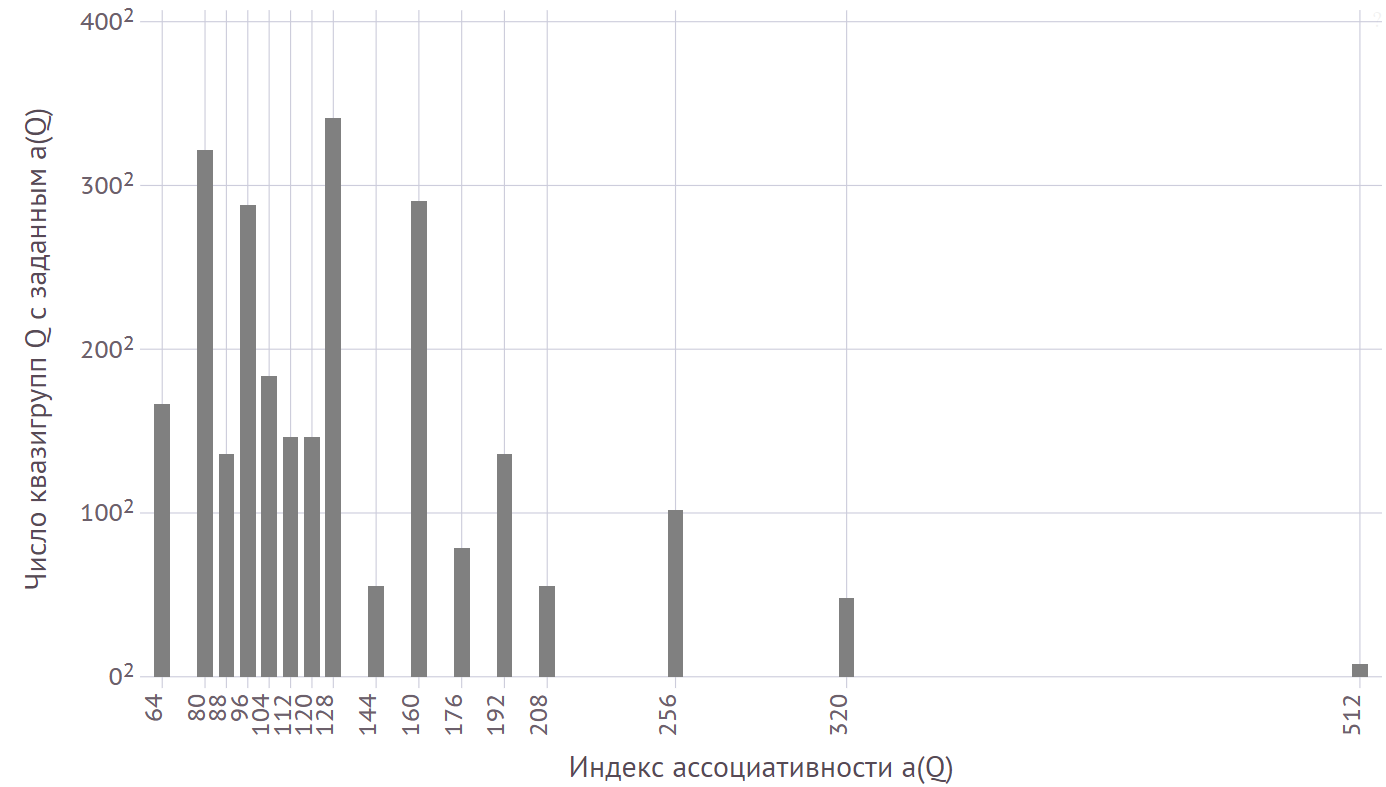
\includegraphics[width=1\linewidth]{histogram.png}
            \caption{Распределение числа квазигрупп с заданным $a(Q)$ для $n = 3$}\label{fig:histogram}
        }
    \end{figure}



    \begin{figure}[ht] % Рисунок
        \centerfloat{
            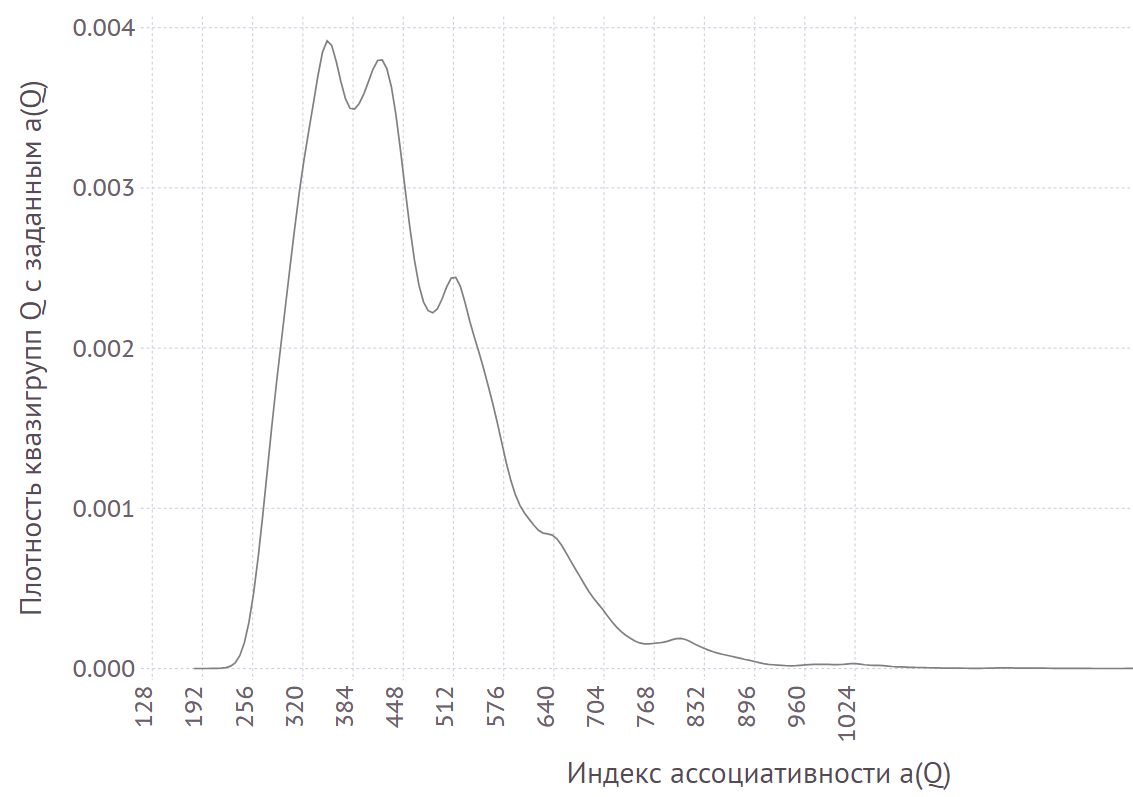
\includegraphics[width=1\linewidth]{density.png}
            \caption{Оценка плотности распределения квазигрупп, построенных по парам правильных булевых семейств, с заданным $a(Q)$ для $n = 4$}\label{fig:density}
        }
    \end{figure}

    Заметим, что при $n = 2$ достигается минимально возможное значение индекса ассоциативности для квазигрупп порядка 4 (а именно 16).
    При~$n \ge 3$ все полученные индексы ассоциативности существенно превышают минимальные теоретически возможные для квазигрупп заданного порядка.
    Отметим также, что во всех исследованных случаях $n = 2, 3, 4$ минимально достижимый индекс ассоциативности у построенных квазигрупп оказался равным квадрату порядка квазигруппы, в связи с чем можно выдвинуть гипотезу, что у квазигрупп, построенным по парам правильных булевых семейств размера $n$ число ассоциативных троек не может быть меньше, чем $2^{2n}$.

    \begin{figure}[ht] % Рисунок
        \centerfloat{
            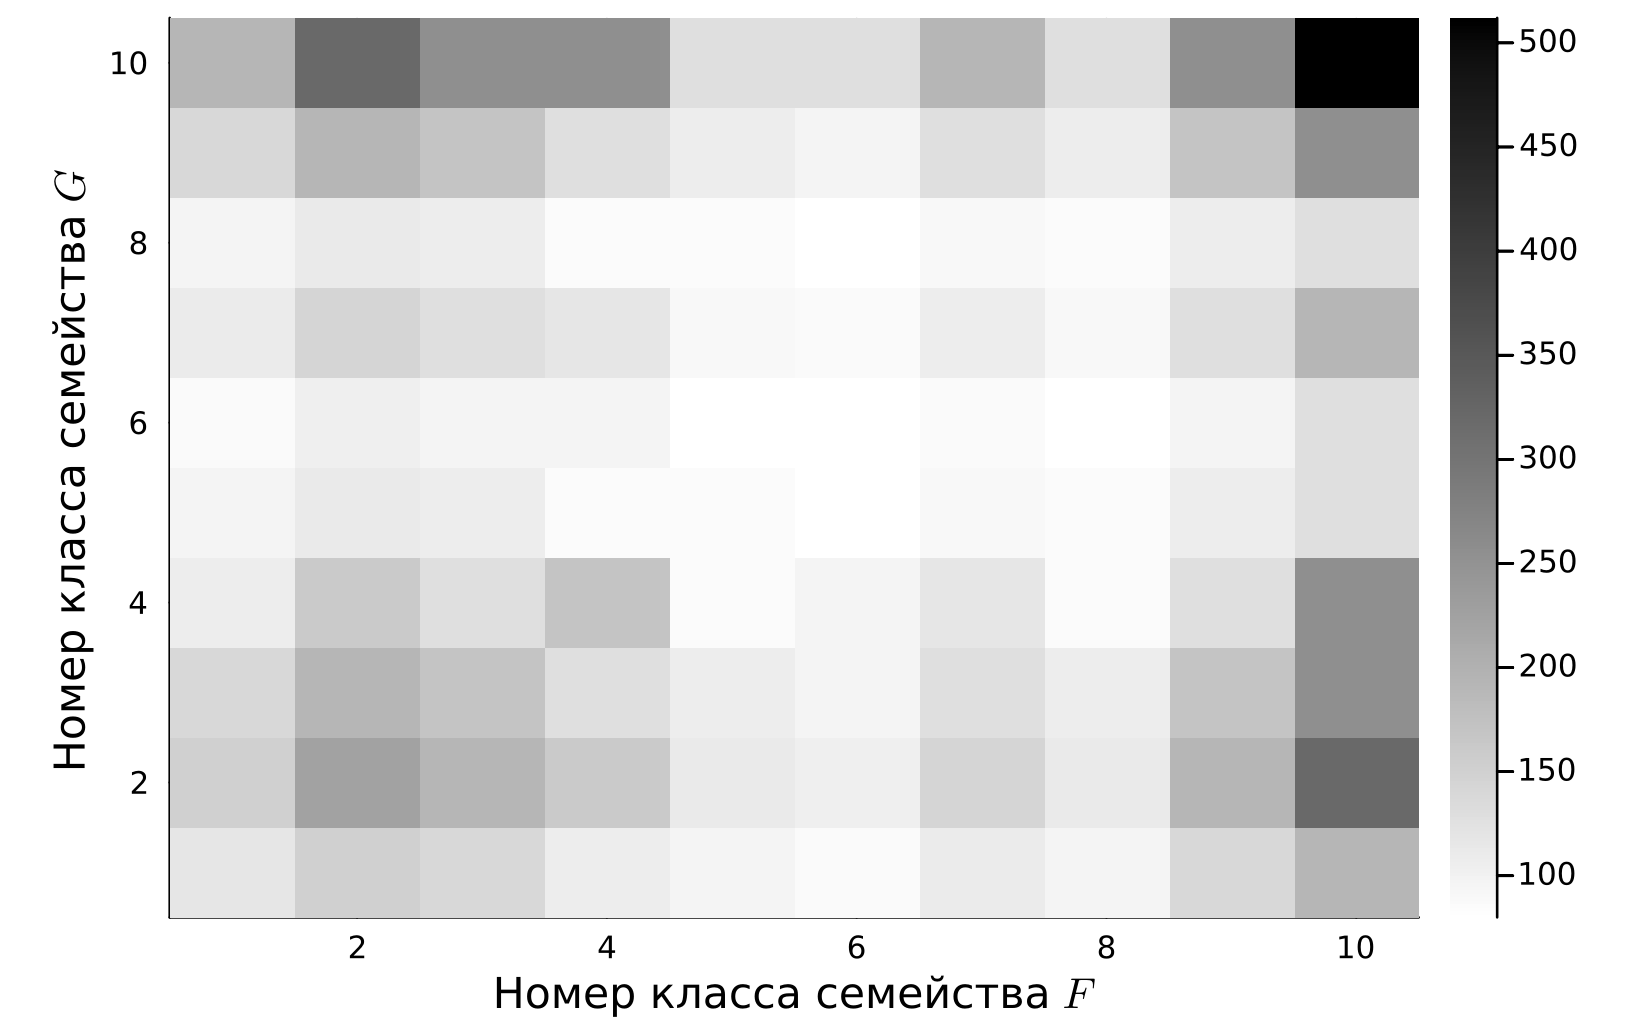
\includegraphics[width=1\linewidth]{heatmap.png}
            \caption{Тепловая карта для среднего индекса ассоциативности, усреднение берется по представителям классов эквивалентности, $n = 3$}\label{fig:heatmap}
        }
    \end{figure}

    Для $n=3$ также был проведен следующий эксперимент.
    Все $744$ правильных семейства были разбиты на $10$ классов эквивалентности относительно изометрий пространства Хэмминга (см. таблицу~\ref{tab:countclasses}).
    Затем для каждой пары классов эквивалентности $(F, G)$ перебирались все пары представителей $\ff \in F$, $\gf \in G$ и вычислялся индекс ассоциативности квазигруппы, порождаемой парой правильных булевых семейств $(\ff, \gf)$, после чего вычислялся <<средний индекс ассоциативности>> для пары классов эквивалентности $(F, G)$.
    Результаты эксперимента отображены на рис.~\ref{fig:heatmap}.
    Из приведенной тепловой карты видно, что наиболее неассоциативные квазигруппы порождаются при использовании $6$-го класса эквивалентности, представителем которого является, например, семейство 
    \[
        \left( x_2 x_3, \; x_1 \oplus x_1 x_3, \; x_1 \oplus x_2 \oplus x_1 x_2 \right). 
    \]
    Представители указанного класса изучались в разделе~\ref{sec:quadfamily}: было показано, что представители класса имеют полный граф существенной зависимости, а также изучалось свойство сильной квадратичности (см. теорему~\ref{thm:strongquad}).



\section{Построение правильных семейств}

    \TODO{расширить: замощения плоскости -- извлечь алгоритм порождения новых правильных семейств?}


\section*{Выводы}

    В настоящей главе были рассмотрены некоторые вопросы, связанные с вычислительными аспектами (алгоритм проверки правильности булева отображения, алгоритм порождения системы представителей), а также приведены результаты некоторых статистических и численных экспериментов.
    Также был предложен к рассмотрению алгоритм шифрования, сохраняющего формат сообщений.




% \subsection{Число ассоциативных троек для квазигрупп, заданных правильными семействами булевых функций}


% На множестве всех правильных семейств можно задать действие группы
% $\mathbb{Z}_2^n$ (см. теорему~\ref{thm:additivity}):
% \[
%     F \to F \oplus A
% \]

% Такое действие сохраняет число ассоциативных троек, заданных правильным семейством, 
% поэтому задача поиска числа ассоциативных троек для правильных семейств заданного размера сводится 
% к перебору орбит данного действия.

% Для правильных семейств булевых функций путем перебора неэквивалентных правильных семейств 
% были получены точные оценки минимального числа ассоциативных троек 
% для семейств размера ${m = 1, \ldots 4.}$ 
% Для $m = 5$ была получена оценка сверху. 
% Напомним, что для правильного семейства размера $m$ латинский квадрат, полученный с помощью этого семейства, имеет размер $n = 2^m.$

% \begin{table}[H]
%     \caption{Минимальное число ассоциативных троек для квазигрупп, 
%     порожденных правильными семействами булевых функций размера ${m \le 5}$}
%     \label{tab2}
%     \begin{center}
%     \begin{tabular}{c|c}
%         $n = 2^m$ & $a^*(n)$ \\ 
%         \hline
%         2 & 8 \\
%         4 & 32  \\
%         8 & 88 \\
%         16 & 256 \\
%         32 & $\le 1120$\\
%     \end{tabular}
%     \end{center}
% \end{table}

% Было получено количество правильных семейств, на которых достигается минимальное число ассоциативных троек. 
% При $m = 2$ минимальное число ассоциативных троек достигается на одной орбите (8 правильных семейств), представитель 
% \[
% \begin{bmatrix}
%     f_1(x_1, x_2) \\ 
%     f_2(x_1, x_2) 
% \end{bmatrix} = 
% \begin{bmatrix}
%     0 \\ 
%     x_1 
% \end{bmatrix}.
% \]

% При $m = 3$ минимальное число 
% ассоциативных троек достигается на 
% двух орбитах (64 правильных семейства), представители: 
% \[
%     \begin{bmatrix}
%         f_1(x_1, x_2, x_3) \\ 
%         f_2(x_1, x_2, x_3) \\ 
%         f_3(x_1, x_2, x_3) 
%     \end{bmatrix} = 
%     \begin{bmatrix} 
%         x_2x_3 \\ 
%         x_1 \oplus x_1x_3 \\ 
%         x_1 \oplus x_2 \oplus x_1x_2 
%     \end{bmatrix}
% \]

% \[
%     \begin{bmatrix}
%         f_1(x_1, x_2, x_3) \\ 
%         f_2(x_1, x_2, x_3) \\ 
%         f_3(x_1, x_2, x_3) 
%     \end{bmatrix} = 
%     \begin{bmatrix} 
%         x_2 \oplus x_2x_3 \\ 
%         x_3 \oplus x_1x_3 \\ 
%         x_1 \oplus x_1x_2 
%     \end{bmatrix}
% \]

% При $m = 4$ минимальное число ассоциативных троек 
% достигается на 56 орбитах (21504 правильных семейств).


% Количество ассоциативных троек в латинском квадрате,
% построенном по правильному семейству,
% сильно зависит от вида параметрических функций $\pi_i$ 
% в определении правильного семейства. 
% В частности, если положить все 
% $\pi_i(x_i, y_i) = a_i, a_i \in \mathbb{Z}_2, $
% то построенный латинский квадрат будет задавать 
% полностью ассоциативную структуру,
% и число ассоциативных троек, соответственно, 
% будет равно $(2^m)^3,$
% где $m$ --- размер правильного семейства.

% Для криптографических приложений желательно, 
% чтобы число параметрических подстановок 
% $\pi_i, \; i = 1, \ldots, n,$
% для которых число ассоциативных троек минимально, 
% было как можно больше.
% С этой целью было проанализировано количество 
% параметрических подстановок,
% на которых достигается минимальное число ассоциативных троек. 
% Для $m = 3$ для каждой функции из двух орбит 
% существует 36 параметрических подстановок,
% на которых достигается нижняя оценка числа ассоциативных троек. 
% Данные параметрические подстановки могут быть различны 
% для функций из одной и той же орбиты.

% Для $m = 4$ для 16 орбит (из 56) существует 
% только 2 параметрические подстановки,
% на которых достигается нижняя оценка числа ассоциативных троек,
% для 32 орбит существует 4 таких подстановки, 
% для 8 орбит существует 8 подстановок.  

% Дополнительно можно отметить,
% что минимальное число ассоциативных троек 
% для заданного семейства при $m = 2, 3, 4$ всегда чётно.           % Глава 4
\chapter*{Заключение}                       % Заголовок
\addcontentsline{toc}{chapter}{Заключение}  % Добавляем его в оглавление

%% Согласно ГОСТ Р 7.0.11-2011:
%% 5.3.3 В заключении диссертации излагают итоги выполненного исследования, рекомендации, перспективы дальнейшей разработки темы.
%% 9.2.3 В заключении автореферата диссертации излагают итоги данного исследования, рекомендации и перспективы дальнейшей разработки темы.
%% Поэтому имеет смысл сделать эту часть общей и загрузить из одного файла в автореферат и в диссертацию:

Основные результаты работы заключаются в следующем.
%% Согласно ГОСТ Р 7.0.11-2011:
%% 5.3.3 В заключении диссертации излагают итоги выполненного исследования, рекомендации, перспективы дальнейшей разработки темы.
%% 9.2.3 В заключении автореферата диссертации излагают итоги данного исследования, рекомендации и перспективы дальнейшей разработки темы.

    \begin{enumerate}
        \item Установлено естественное соответствие между булевыми правильными семействами и одностоковыми ориентациями графов булевых кубов ($\uso$-ориентации).
        \item Установлено естественное соответствие между булевыми правильными семействами и булевыми сетями с наследственно единственной неподвижной точкой ($\hupf$-сети).
        \item Установлено естественное соответствие между правильными семействами в логике произвольной значности и кликами в обобщенных графах Келлера.
        \item Доказано, что стабилизатором множества правильных семейств функций являются изометрии пространства Хэмминга (согласованные перенумерации и перекодировки).
        \item Показано, что отображения, задаваемые с помощью правильных семейств булевых функций, всегда имеют четное число неподвижных точек.
        \item Получена оценка на число правильных семейств булевых функций, предложены оценки доли треугольных семейств среди всех правильных семейств булевых функций.
        \item Обнаружены и исследованы новые классы правильных семейств функций (рекурсивно треугольные, локально треугольные, сильно квадратичное семейство).
        \item Получены оценки на число рекурсивно треугольных семейств.
        \item Для некоторых правильных семейств булевых функций получены точные значения мощности образа отображений, задаваемых этими правильными семействами.
        \item Предложен новый способ порождения квазигрупп на основе правильных семейств функций.
        \item Доказан ряд утверждений о числе ассоциативных троек в порождаемых квазигруппах.
        \item Предложен новый алгоритм шифрования, сохраняющего формат ($\fpe$-схема), основанный на квазигрупповых операциях.
    \end{enumerate}

    В качестве тем для дальнейших исследований можно отметить следующие направления.

    \begin{enumerate}
        \item Предложить способ построения достаточно широких классов правильных семейств с хорошими алгебраическими и комбинаторными свойствами, в том числе и для логик большей значности $k > 2$.

        \item Предложить способ быстрого построения множества представителей всех правильных семейств размера $n+1$ с помощью представителей размера $n$ и менее (с точностью до согласованных перенумераций и перекодировок).

        \item Предложить альтернативные геометрические описания правильных семейств в $k$-значной логике, где $k>2$, которые были бы инвариантны относительно согласованных перенумераций и перекодировок.

        \item Предложить алгоритм, полиномиальный по длине входа, на вход принимающий правильное семейство (например, в виде КНФ или полиномов Жегалкина) и параметрические подстановки и выдающий количество ассоциативных троек (или нижние и верхние границы на число троек), проверяющий полиномиальную полноту порождаемой квазигруппы, наличие или отсутствие подквазигрупп.

        \item Оценить генерическую сложность задачи решения системы уравнений над квазигруппами, заданными правильными семействами.
    \end{enumerate}

Автор выражает глубокую благодарность своему научному руководителю А.~Е.~Панкратьеву  и с.н.с. А.~В.~Галатенко за оказанную помощь при написании настоящей работы, постановку задачи, обсуждение результатов и постоянное внимание к работе.
      % Заключение
\printnomenclature[3.5cm] % Значение ширины столбца с обозначениями стоит подбирать вручную
        % Список сокращений и условных обозначений
% \chapter*{Словарь терминов}             % Заголовок
% \addcontentsline{toc}{chapter}{Словарь терминов}  % Добавляем его в оглавление

% \textbf{TeX} : Cистема компьютерной вёрстки, разработанная американским профессором информатики Дональдом Кнутом

% \textbf{панграмма} : Короткий текст, использующий все или почти все буквы алфавита
      % Словарь терминов
\clearpage                                  % В том числе гарантирует, что список литературы в оглавлении будет с правильным номером страницы
%\hypersetup{ urlcolor=black }               % Ссылки делаем чёрными
%\providecommand*{\BibDash}{}                % В стилях ugost2008 отключаем использование тире как разделителя
\urlstyle{rm}                               % ссылки URL обычным шрифтом
\ifdefmacro{\microtypesetup}{\microtypesetup{protrusion=false}}{} % не рекомендуется применять пакет микротипографики к автоматически генерируемому списку литературы
\insertbibliofull                           % Подключаем Bib-базы: все статьи единым списком
% Режим с подсписками
%\insertbiblioexternal                      % Подключаем Bib-базы: статьи, не являющиеся статьями автора по теме диссертации
% Для вывода выберите и расскомментируйте одно из двух
%\insertbiblioauthor                        % Подключаем Bib-базы: работы автора единым списком 
%\insertbiblioauthorgrouped                 % Подключаем Bib-базы: работы автора сгруппированные (ВАК, WoS, Scopus и т.д.)
\ifdefmacro{\microtypesetup}{\microtypesetup{protrusion=true}}{}
\urlstyle{tt}                               % возвращаем установки шрифта ссылок URL
%\hypersetup{ urlcolor={urlcolor} }          % Восстанавливаем цвет ссылок
      % Список литературы
\clearpage
\ifdefmacro{\microtypesetup}{\microtypesetup{protrusion=false}}{} % не рекомендуется применять пакет микротипографики к автоматически генерируемым спискам
\listoffigures  % Список изображений

%%% Список таблиц %%%
% (ГОСТ Р 7.0.11-2011, 5.3.10)
\clearpage
\listoftables   % Список таблиц
\ifdefmacro{\microtypesetup}{\microtypesetup{protrusion=true}}{}
\newpage           % Списки таблиц и изображений (иллюстративный материал)

\setcounter{totalchapter}{\value{chapter}} % Подсчёт количества глав

%%% Настройки для приложений
\appendix
% Оформление заголовков приложений ближе к ГОСТ:
\setlength{\midchapskip}{20pt}
\renewcommand*{\afterchapternum}{\par\nobreak\vskip \midchapskip}
\renewcommand\thechapter{\Asbuk{chapter}} % Чтобы приложения русскими буквами нумеровались

% \begin{frame}
%     \frametitle{Ответы на замечания ведущей организации НИИ~<<Рога~и~копыта>>}
%     \begin{itemize}
%         \item Замечание -- ответ
%         \item Замечание -- ответ
%         \item Замечание -- ответ
%         \item Замечание -- ответ
%         \item Замечание -- ответ
%     \end{itemize}
% \end{frame}
% 
% \begin{frame}
%     \frametitle{Ответы на замечания оф. оппонента Иванова\,И.\,И}
%     \begin{itemize}
%         \item Замечание -- ответ
%         \item Замечание -- ответ
%         \item Замечание -- ответ
%         \item Замечание -- ответ
%         \item Замечание -- ответ
%     \end{itemize}
% \end{frame}
% 
% \begin{frame}
%     \frametitle{Ответы на замечания Петрова\,П.\,П}
%     \begin{itemize}
%         \item Замечание -- ответ
%         \item Замечание -- ответ
%         \item Замечание -- ответ
%         \item Замечание -- ответ
%         \item Замечание -- ответ
%     \end{itemize}
% \end{frame}
        % Приложения

\setcounter{totalappendix}{\value{chapter}} % Подсчёт количества приложений

\end{document}
